\documentclass[10pt,twoside,openright]{report}
\usepackage[T1]{fontenc}
\usepackage[utf8]{inputenc}
\usepackage[francais]{babel}
\usepackage{amsmath}
\usepackage{graphicx}
\graphicspath{{Figures/}}
\usepackage[backend=biber,style=authoryear,bibencoding=utf8]{biblatex}
\usepackage{fancyhdr}
\pagestyle{fancy}
\fancyhead[RO,LE]{}

\usepackage[colorlinks,linkcolor=blue]{hyperref}
\newcommand{\micro}{$\mathrm{\mu}$}
\addbibresource{biblio2.bib}

\title{
	{Thesis Title}\\
	{\large Institution Name}\\
}
\author{Author Name}
\date{\today}


\begin{document}


\begin{abstract}
Abstract
\end{abstract}
\tableofcontents


%\documentclass[10pt,twoside]{report}
%\usepackage[T1]{fontenc}
%\usepackage[utf8]{inputenc}
%\usepackage[francais]{babel}
%\usepackage{amsmath}
%\usepackage{graphicx}
%\graphicspath{{Figures/}}
%\usepackage[backend=biber,style=authoryear,bibencoding=utf8]{biblatex}
%\usepackage{fancyhdr}
%\pagestyle{fancy}
%\fancyhead[RO,LE]{}
%
%\usepackage[colorlinks,linkcolor=blue]{hyperref}
%\newcommand{\micro}{$\mathrm{\mu}$}
%\addbibresource{biblio2.bib}
%
%\begin{document}

\chapter*{Introduction et objectifs}
  Au moment où s'achève l'écriture de ce manuscrit, se déroule le Tour de France cycliste. En observant les jambes des coureurs, il est parfois difficile de se dire qu'elles sont formées sur la même base que les nôtres. Si l'on peut se douter qu'un champion doit être doté d'une conjonction de caractéristiques génétiques particulières et d'années de travail, il demeure que la plupart d'entre nous, même sans don particulier, peut atteindre des performances sportives étonnantes après un entraînement rigoureux. C'est que notre corps est adaptable, et en particulier nos muscles, qui en réponse à des sollicitations répétées, vont devenir plus forts, plus rapides, plus précis. La musculation constitue l'exemple le plus immédiat et quotidien de la mécanotransduction, cette capacité qu'a notre corps d'interpréter de manière biologique un signal mécanique, et d'y apporter une réponse. Cette capacité se retrouve à toutes les échelles de l'organisme, de l'organe à la cellule qui le compose. 
  
  Cette thèse s'intéresse tout particulièrement à ce phénomène de mécanotransduction à l'échelle de la cellule musculaire. Les cellules d'un muscle en exercice sont soumises à des forces extérieures, elles vont y réagir en formant plus de masse musculaire. Ce champ de recherche se place alors naturellement à la rencontre de la physique, qui étudie particulièrement les forces mécaniques, et de la biologie cellulaire. 
  
  Le premier chapitre de cette thèse sera consacré à la description rapide de la cellule animale, des éléments qui la composent et de leur fonctionnement. 

	Les cellules maintiennent leur forme, se déplacent, se divisent grâce à un réseau de filaments appelé cytosquelette. Ce cytosquelette est essentiel dans la réponse des cellules aux forces extérieures, et détermine en grande partie leur réponse mécanique. L'actine est une protéine du cytosquelette, présente en grande quantité dans les cellules musculaires, qui est à la fois un acteur majeur des propriétés rhéologiques de la cellule et de la contraction musculaire. Elle peut former des filaments semi-rigides, dans une structure dynamique toujours en construction et déconstruction, formant un équilibre entre l'actine seule (en monomères) et l'actine incorporée dans les filaments.  Le deuxième chapitre sera consacré à la description de l'actine et des structures qu'elle forme dans la cellule. 

  À l'aide d'études sur des souris, l'équipe d'Athanassia Sotiropoulos a mis en évidence le rôle d'une voie de signalisation dans l'hypertrophie et l'atrophie des muscles en réponse à une contrainte mécanique. Le facteur de transcription Serum Response Factor, qui contrôle les gènes du cytosquelette et de la différenciation musculaire, et son cofacteur Myocardin-Related Transcription Factor, sont les deux acteurs centraux de ce phénomène. Or il a déjà été montré que MRTF-A est régulée par l'actine. Ensemble ces deux protéines font le pont entre la sensibilité mécanique de la cellule, au niveau du cytosquelette d'actine, et l'activation des gènes par SRF. Le troisième chapitre de cette thèse expliquera en détail le rôle de MRTF-A, et la manière dont cette protéine interagit avec l'actine pour induire une réponse génétique à un stimulus mécanique. 
  
  Dans les cellules musculaires, l'actine est organisée d'une manière extrêmement spécifique, pour permettre la contraction musculaire. Cette organisation sera décrite dans le chapitre 4. 
  
  Enfin, le chapitre 5 sera consacré aux propriétés mécaniques des cellules et du cytosquelette d'actine. Il décrira les outils que les physiciens ont élaboré pour exercer et mesurer des forces à des échelles cellulaire et sub-cellulaire, et les lois mécaniques mises en évidence par ces mesures. 
  
  Ces cinq premiers chapitres dessinent tout le chemin qui se trouve entre le signal mécanique que va sentir la cellule, et la réponse génétique qu'elle va y apporter : une contrainte mécanique peut être à l'origine d'une réorganisation du cytosquelette d'actine, les modifications de ce dernier vont réguler MRTF-A, qui va à son tour contrôler le facteur de transcription SRF, et déclencher l'expression d'un programme génétique. Plus particulièrement, MRTF-A doit être dans le noyau de la cellule pour pouvoir activer le programme génétique avec SRF. Or la localisation de MRTF-A dans la cellule est régulée par la quantité de monomères d'actine disponible. Lorsqu'il y a une grande quantité de monomères, ceux-ci se lient à MRTF-A et l'empêchent d'aller dans le noyau. Au contraire, lorsque les monomères viennent à manquer, MRTF-A peut être importée dans le noyau et y interagir avec SRF. 
  
  L'équipe dans laquelle j'étais en thèse avait déjà constaté auparavant que l'application de contraintes mécaniques répétées sur une cellule musculaire induit une polymérisation du cytosquelette d'actine en réponse. Cela, associé aux résultats de l'équipe de l'Institut Cochin, conduit à formuler l'hypothèse suivante : lorsque les cellules musculaires sont soumises à des forces extérieures, leur cytosquelette d'actine se renforce en polymérisant, cette polymérisation d'actine conduit à un manque de monomères pour se lier à MRTF-A, qui est alors libre d'aller dans le noyau se lier à SRF, pour activer le programme génétique de développement musculaire. 
  
  L'objectif de ce travail est d'étudier comment les signaux mécaniques vont réguler MRTF-A à travers les modifications du cytosquelette d'actine. Pour cela, la première étape a été de construire des outils nous permettant d'exercer des forces à l'échelle de la cellule unique, et de mesurer leur réponse mécanique et biologique. Les pinces magnétiques ont permis de caractériser la rhéologie des cellules musculaires, et d'observer la réponse biologique de MRTF-A. L'étireur de cellules a permis d'étudier de manière systématique sur une grande population de cellules la réponse du système à des déformations imposées. Les techniques de microscopie de fluorescence ont été utilisées pour visualiser les deux protéines, actine et MRTF-A, à l'intérieur de la cellule. Toutes ces méthodes expérimentales sont décrites en détail dans le chapitre 6. 
  
  À l'aide de ces outils, nous avons pu caractériser les propriétés mécaniques de myoblastes, qui seront présentées au chapitre 7. 
  
  Enfin, au chapitre 8, nous montrerons que l'application de contraintes mécaniques peut induire une polymérisation ou une dépolymérisation du cytosquelette d'actine, conduisant à des changements de localisation de MRTF-A dans les cellules. Nous verrons également que l'utilisation de marqueurs du cytosquelette perturbe l'équilibre entre les filaments d'actine et les monomères d'une manière qui est toujours perceptible dans la localisation de MRTF-A. 





%\end{document}

%\documentclass{report}
%\usepackage[T1]{fontenc}
%\usepackage[utf8]{inputenc}
%\usepackage[francais]{babel}
%\usepackage{amsmath}
%\usepackage{graphicx}
%\graphicspath{{Figures/}}
%\usepackage[backend=biber,style=authoryear,bibencoding=utf8]{biblatex}
%\usepackage[colorlinks,linkcolor=blue]{hyperref}
%
%
%\addbibresource{biblio2.bib}
%
%\begin{document}
\chapter{La cellule}
\begin{center}
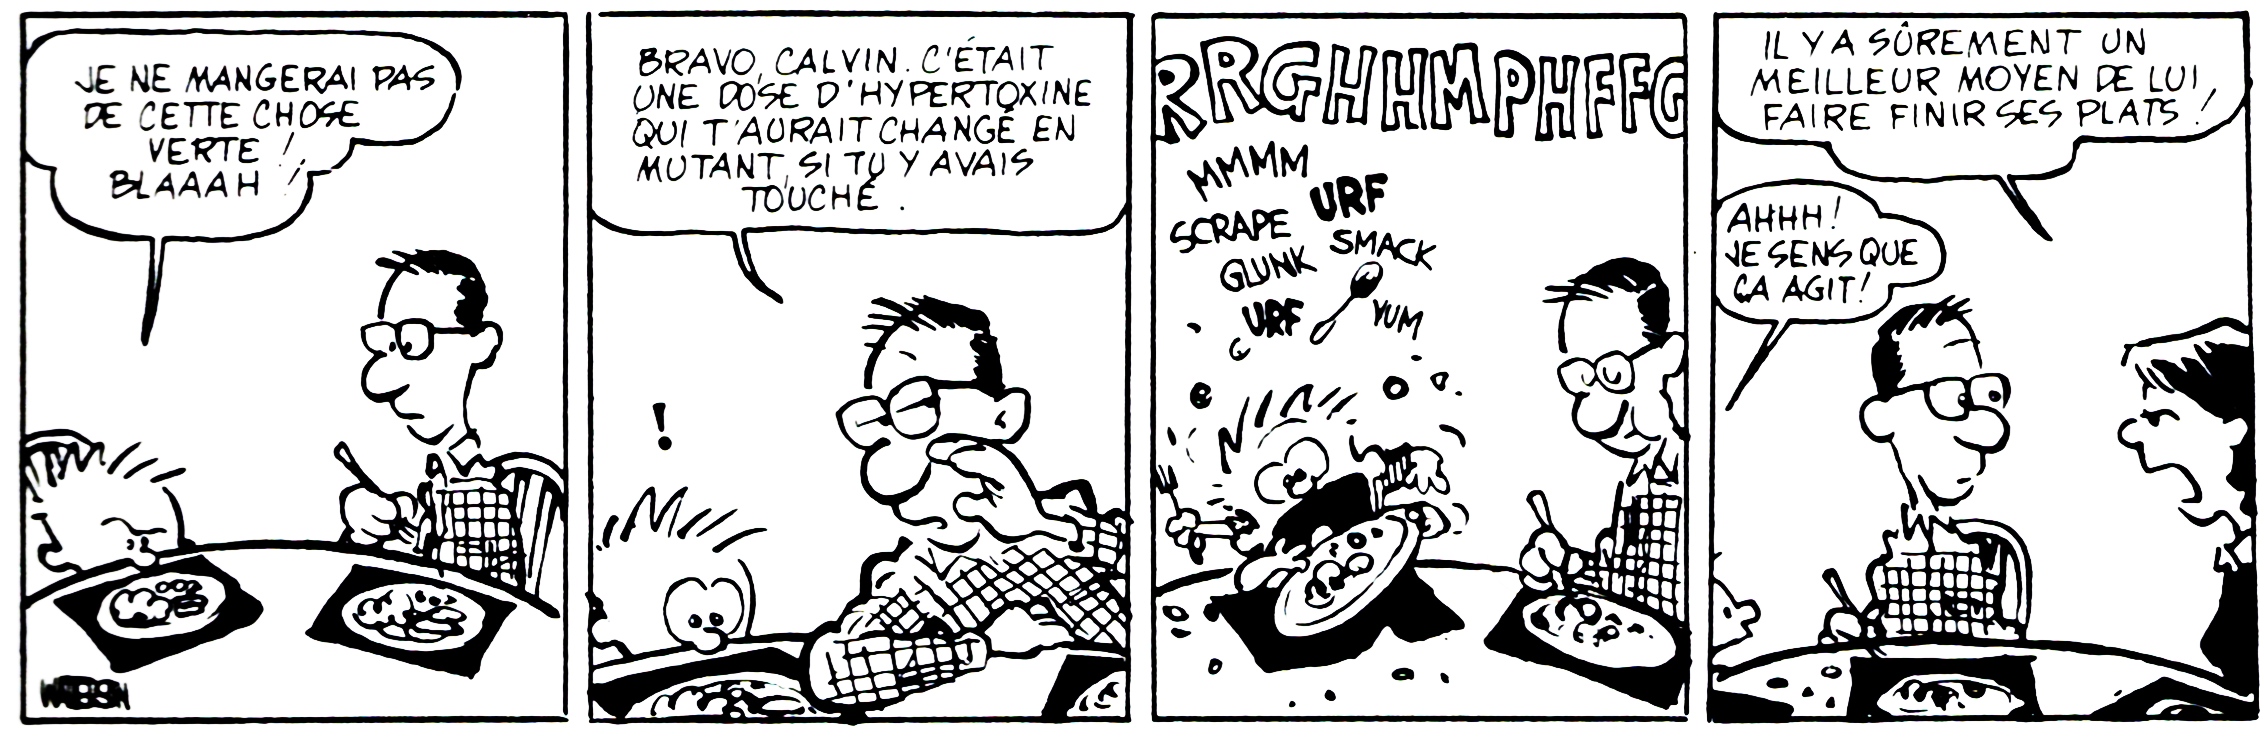
\includegraphics[scale=0.7]{Chapitre1.png}
\end{center}

\newpage

La cellule est l'unité de base des êtres vivants. Elle peut puiser de l'énergie du milieu extérieur afin de se maintenir dans un état organisé et de se reproduire pour donner naissance à d'autres cellules par la division cellulaire. 

Une cellule est séparée du milieu extérieur par une membrane. Elle contient son code génétique sous la forme d'ADN, elle le duplique et le transmet lors de ses divisions. 

Les cellules sont séparées en deux grands groupes en fonction de l'état de leur ADN : les procaryotes et les eucaryotes. 
L'ADN des procaryotes est libre dans la cellule, il est souvent constitué d'un seul chromosome circulaire. 
Au contraire, l'ADN des eucaryotes est confiné dans un compartiment spécial, le noyau. 

Chez les eucaryotes comme chez les procaryotes, il existe des organismes vivants pouvant être composés d'une ou de plusieurs cellules (\cite{grosberg_evolution_2007}).
Les plus grands organismes, comme les plantes ou les animaux, peuvent être composées d'un très grand nombre de cellules (de l'ordre de $10^{14}$) qui possèdent le même génome mais ont des phénotypes très divers. 

\section{Organisation de la cellule eucaryote}
\begin{figure}[h!]
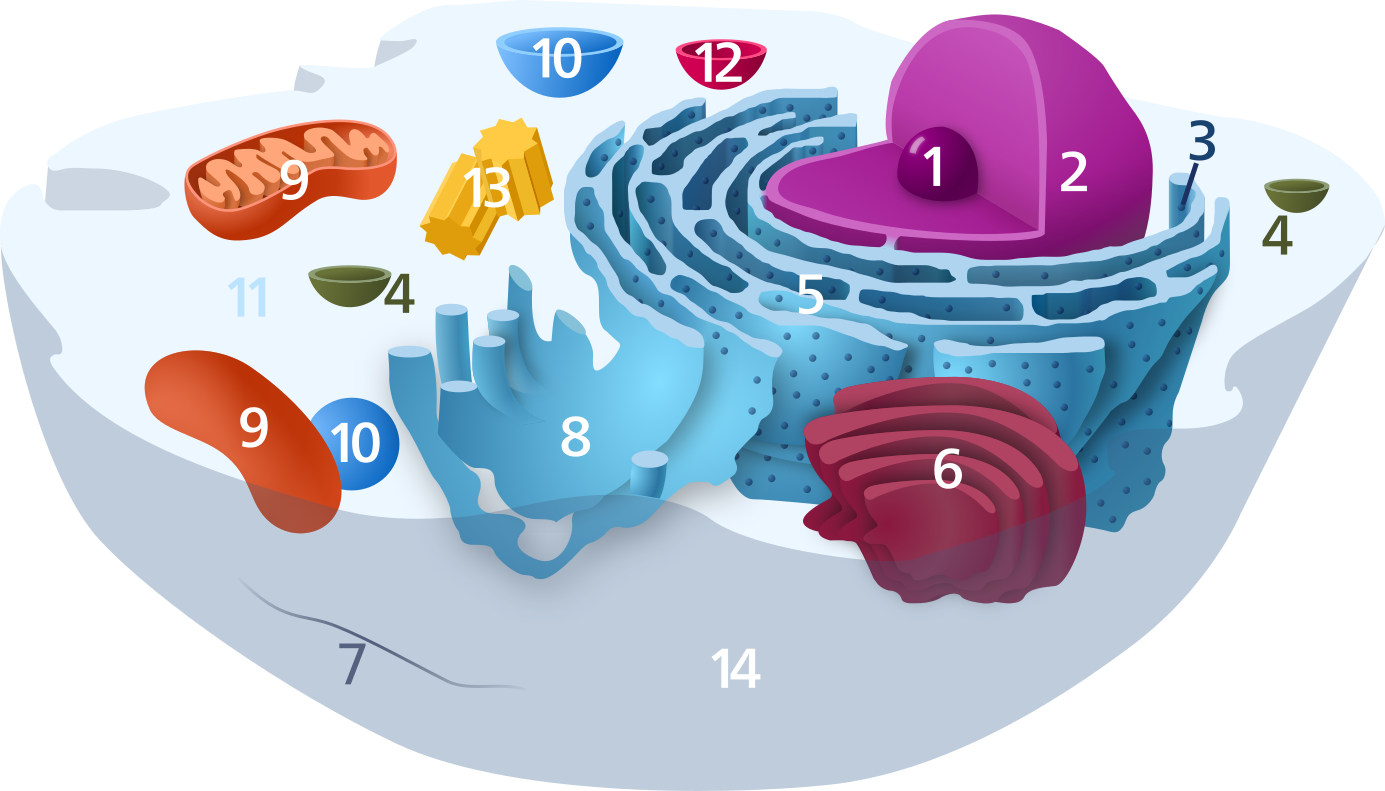
\includegraphics[scale=0.2]{Animal_Cell.png}
\caption{La cellule eucaryote. 
1. Nucléole
2. Noyau
3. Ribosome
4. Vésicule
5. Réticulum endoplasmique rugueux
6. Appareil de Golgi
7. Cytosquelette
8. Réticulum endoplasmique lisse
9. Mitochondrie
10. Vacuole (cellule végétale uniquement)
11. Cytosol
12. Lysosome
13. Centrosome
14. Membrane Plasmique
Figure par Kelvinsong (CC0)}
\end{figure}


Les cellules eucaryotes sont composées de plusieurs compartiments aux fonctions spécifiques à l'intérieur d'une membrane plasmique. Le noyau est le plus gros de ces compartiments, il renferme l'ADN organisé sous la forme de chromosomes et est le lieu de la transcription de l'ADN en ARN. 
Le réticulum endoplasmique rugueux est le siège de la traduction de l'ARN en protéines. 
L'appareil de Golgi est le lieu de transformation finale des protéines. 
Les mitochondries sont les unités de production d'énergie de la cellule : elles produisent l'Adénosine Triphosphate (ATP), qui sera transformée en Adénosine Diphosphate (ADP) en libérant de l'énergie. Les mitochondries seraient d'anciennes bactéries devenues symbiotiques des cellules eucaryotes, elles possèdent leur propre ADN. 

\subsection{L'énergie dans la cellule}

Une cellule vivante est un système très éloigné de l'équilibre thermodynamique. Pour se maintenir en vie, elle utilise donc de l'énergie qu'elle va trouver dans le milieu extérieur. 

À l'intérieur de la cellule, la source d'énergie utilisée dans les réactions enzymatiques est l'hydrolyse de nucléosides triphosphates. 
Il s'agit majoritairement d'Adénosine Triphosphate, qui est hydrolysée en Adénosine Diphosphate et un phosphate inorganique en libérant de l'énergie. 
Les protéines qui utilisent l'ATP comme source d'énergie sont des ATPases. 
C'est le cas par exemple de l'actine lors de sa polymérisation et de la myosine  lors de la contraction musculaire, dont nous ferons une description plus détaillée plus loin. 

Certaines protéines utilisent à la place de l'ATP le Guanosine Triphosphate, fonctionnant de la même manière. 
C'est par exemple le cas des microtubules ou des petites GTPases comme RhoA, dont nous parlerons également plus loin. 

L'ATP ne peut pas être puisée directement dans le milieu extérieur. Les sources d'énergie des cellules animales sont les glucides simples (comme les sucres) ou complexes (comme l'amidon) et les lipides ou les acides aminés lorsque les autres sources font défaut. 

La cellule animale reçoit principalement son énergie sous forme de glucose par la circulation sanguine. Ce glucose est alors dégradé d'abord dans le cytoplasme, puis en présence de dioxygène dans la mitochondrie. 
Une molécule de glucose permet d'obtenir une trentaine d'ATP. 
Lorsque le dioxygène vient à manquer, par exemple lors d'efforts musculaires intenses, la fermentation permet de produire de l'énergie à partir du glucose en produisant de l'acide lactique. 

\subsection{Le noyau}

Le noyau est l'organite contenant le matériel génétique de la cellule sous la forme d'ADN (à l'exception de l'ADN mitochondrial). Cependant, bien d'autres molécules que l'ADN sont présentes dans le noyau, et il s'y passe d'autres choses que la transcription ou la duplication de l'ADN. 

\subsubsection{ADN}

\begin{figure}
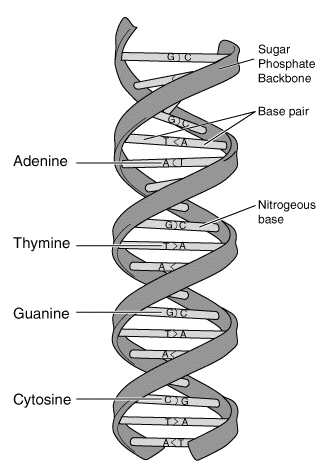
\includegraphics[scale=0.3]{ADN.png}
\caption{Schéma de la structure de l'ADN, par Messer Woland CC-BY-SA-2.5}
\end{figure}

L'ADN est une molécule constituée d'un enchaînement de nucléotides composés d'une base azotée, d'un sucre et d'un groupement phosphate. Il existe quatre bases azotées possibles : Adénine, Thymine, Cytosine, Guanine. Leur enchaînement va être à la base du code génétique.
L'enchaînement des nucléotides forme une double hélice dans laquelle les nucléotides se correspondent en deux paires : Adénine et Thymine, Cytosine et Guanine. 

Le génome des êtres vivants comporte typiquement du million au milliard de paires de base d'ADN. La distance entre deux bases est de 0,34nm. Chez l'homme, on compte environ 3,2 milliards de paires de bases, ce qui correspond à une longueur d'ADN de l'ordre du mètre, qui doit être stockée dans le noyau cellulaire d'un diamètre de 5 à 7 microns. 
On conçoit alors qu'une organisation spécifique de l'ADN dans le noyau soit nécessaire pour faire tenir une molécule aussi grande dans un compartiment aussi étroit. 

\begin{figure}[h!]
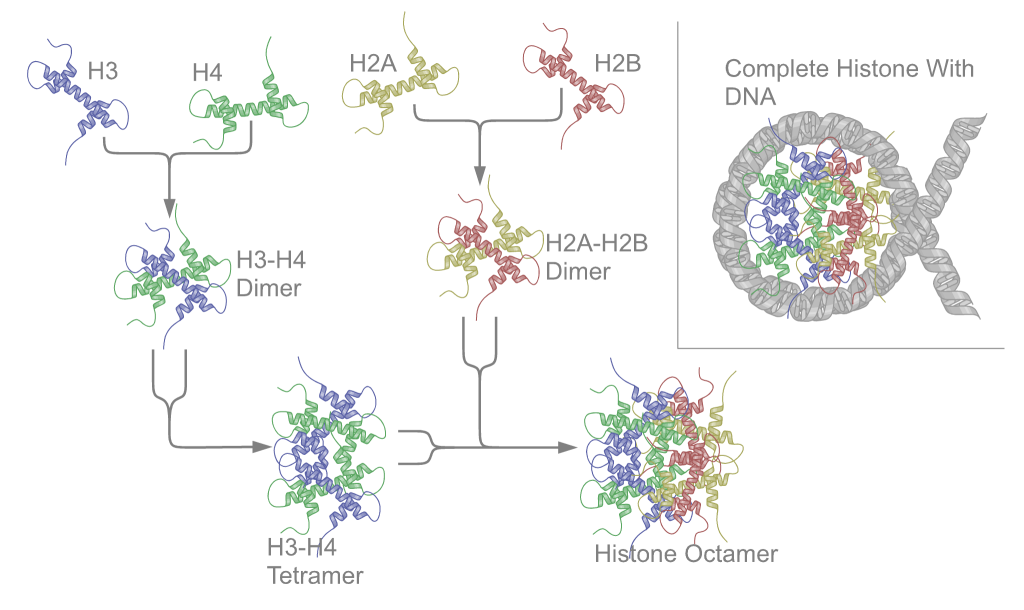
\includegraphics[scale=0.3]{Nucleosome_structure_by_richard_wheeler}
\caption{Enroulement de l'ADN autour d'un complexe d'histones, illustré par Richard Wheeler (CC BY-SA 3.0). Les histones 2A (en jaune) et 2B (en rouge) forment ensemble un dimère, et deux dimères forment un tétramère. Il en est de même pour les histones 3 (en bleu) et 4 (en vert). Un tétramère d'histones 2A/2B et un tétramère d'histones 3/4 s'associent ensemble pour former un octamère complet, qui est donc formé de deux histones de chacun des quatre types, autour duquel l'ADN peut s'enrouler. 
\label{histone}}
\end{figure}

L'ADN est enroulé autour de protéines appelées histones comme du fil autour d'une bobine, formant une structure appelée nucléosome, comme représenté sur la figure \ref{histone}. Ces nucléosomes empilés forment une structure bien plus compacte que l'ADN libre, appelée la chromatine. Certains acides aminés qui composent les histones peuvent subir des réactions chimiques comme l'acétylation ou la méthylation, qui ont un rôle dans la régulation de la transcription du génome. L'acétylation des histones peut changer l'état de la chromatine : l'hétérochromatine est la forme compacte où l'ADN ne peut pas être transcrit, l'euchromatine est la forme plus étendue dans laquelle l'ADN est accessible pour la transcription. 

\subsubsection{Transport nucléo-cytoplasmique}
\begin{figure}
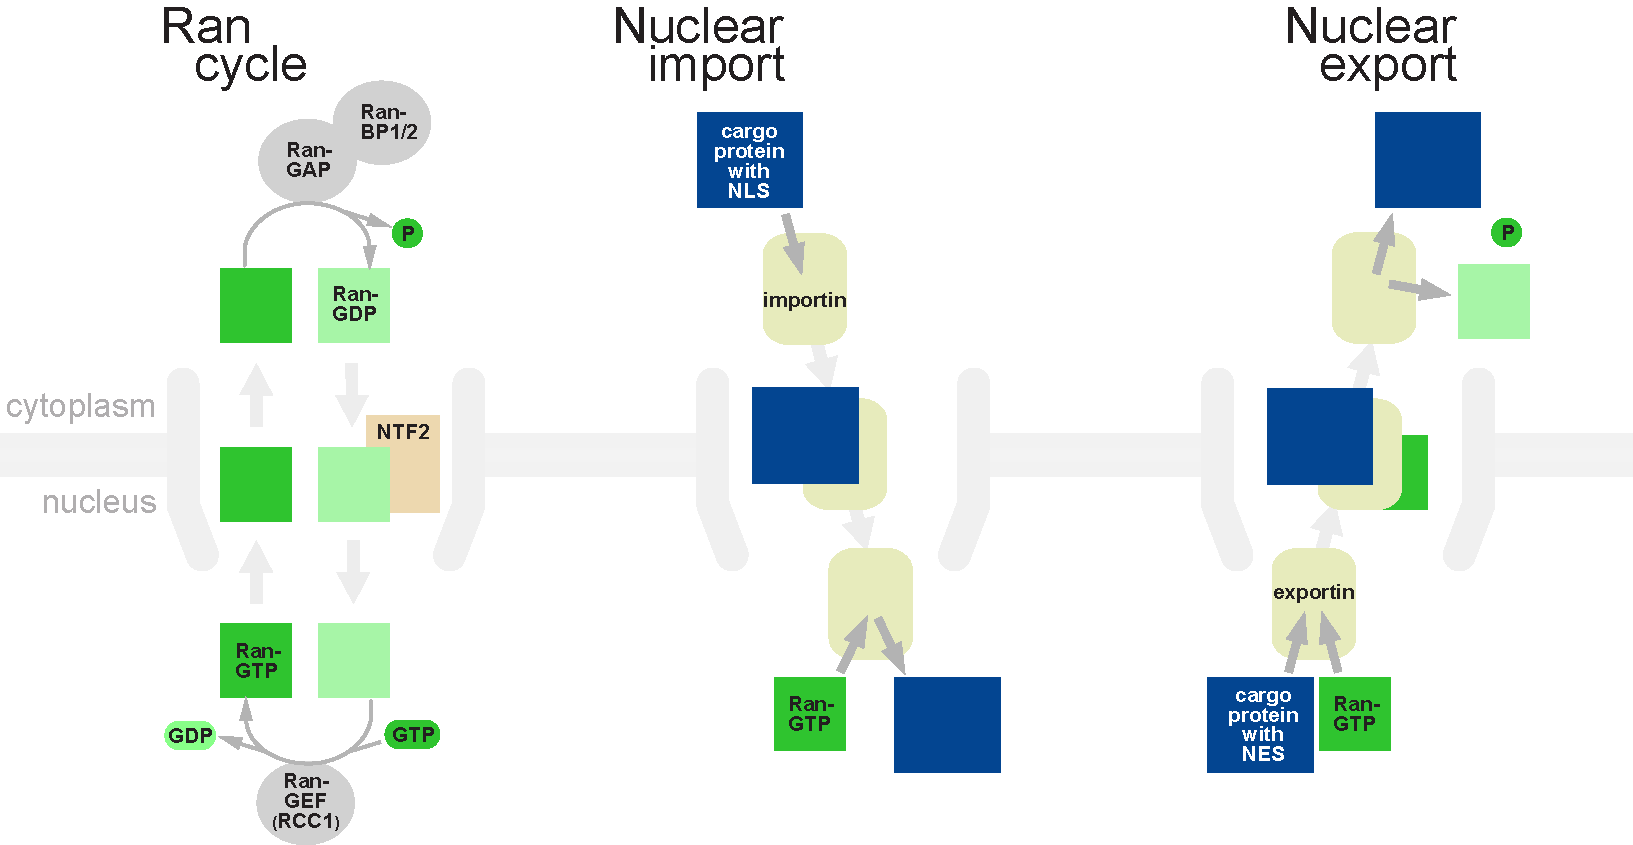
\includegraphics[scale=0.8]{Rancycle_nuclearimport_nuclearexport.png}
\caption{Schéma du transport nucléo-cytoplasmique par les karyophérines. Les importines reconnaissent la séquence NLS sur la protéine à transporter (le cargo) et passent avec elle le pore nucléaire. À l'arrivée, la RanGTP permet de libérer le cargo. Les exportines reconnaissent la séquence NES et s'associent à une RanGTP dans le noyau. Puis elles font passer avec elles le cargo vers le cytoplasme, où le cargo et la RanGTP hydrolysée sont libérées. RanGTP est la GTPase qui fournit l'énergie à ce système d'import actif. \label{import} }
\end{figure}
Le noyau est séparé du reste du cytoplasme par une membrane formée de deux bicouches lipidiques, dont une illustration détaillée est visible plus loin en figure \ref{membrane nucléaire}. Elle contient des complexes de protéines qui servent de portes d'entrée et de sortie  et qui sont appelées pores nucléaires. Les protéines de taille inférieure à 40 kDa peuvent passer par diffusion passive par les pores nucléaires. 

Les protéines de plus grande taille doivent faire appel à des transporteurs spécifiques pour aller d'un côté de la membrane à l'autre (illustration en figure \ref{import}. 
Les importines se lient à la protéine à importer au niveau d'une zone appelée \og Signal de Localisation Nucléaire \fg (NLS). L’importine interagit avec le pore nucléaire et le couple importine-cargo va ainsi passer à travers le pore nucléaire. 
Une fois dans le noyau, l'importine va se lier à la RanGTP et se dissocier du cargo, qui est libéré dans le nucléoplasme. L'importine est alors à nouveau exportée du noyau et la GTP hydrolysée en GDP. 
De même, une protéine possédant une séquence d'export nucléaire (NES) sera liée à une exportine-GTP, et le couple pourra passer vers le cytoplasme. Une fois dans le cytoplasme, la GTP est hydrolysée en GDP et le cargo relargué. L'exportine revient dans le noyau par diffusion. 

Par exemple, l'actine, bien que de taille 42kDa, à la limite de la diffusion passive, est importée de manière active par l'importine 9 et exportée par l'exportine 6. 

\subsection{La membrane plasmique}

La membrane plasmique sépare le milieu intérieur de la cellule de l'extérieur. Elle est composée d'une bicouche de phospholipides amphiphiles dans laquelle sont enchâssées des protéines transmembranaires qui permettent de réguler les échanges avec le milieu (figure \ref{membrane}) . 

\begin{figure}
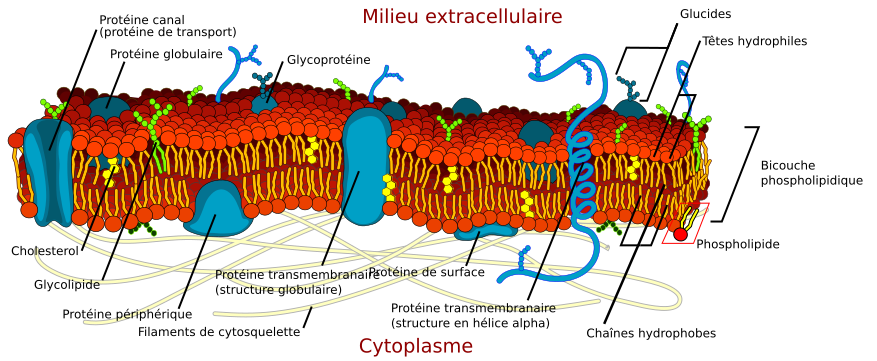
\includegraphics[scale=0.5]{Cell_membrane_detailed_diagram_fr.png}
\caption{Schéma de la membrane plasmique \label{membrane}}
\end{figure}
\subsubsection{Transport transmembranaire}
La membrane permet de réguler le passage de molécules d'un côté à l'autre de manière active ou passive. 
 Il existe une très grande variété de transporteurs d'espèces chimiques à travers la membrane. 

Les lipides peuvent passer par diffusion à travers la membrane plasmique, c'est le cas par exemple des hormones stéroïdiennes comme les androgènes ou les \oe strogènes, dont les récepteurs sont à l'intérieur de la cellule et non sur la membrane.

Les ions comme le calcium, le potassium ou le magnésium sont transportés par des canaux spécifiques. Le mouvement des ions permet de polariser la membrane et de faire passer un signal électrique et est essentiel dans le fonctionnement du système nerveux et dans la contraction musculaire. Des canaux spécialisés, les aquaporines, laissent passer l'eau pour moduler la pression osmotique.

Des molécules peuvent également être transportées de l'extérieur vers l'intérieur par l'invagination d'une partie de la membrane en une petite vésicule. Ce phénomène s'appelle l'endocytose. Inversement, des vésicules dans le milieu intracellulaire peuvent fusionner avec la membrane pour émettre leur contenu vers l'extérieur, c'est l'exocytose. Les cellules fabriquant la matrice extra-cellulaire utilisent l'exocytose pour excréter les protéines synthétisées. 

\subsubsection{Signalisation}

La liaison d'un récepteur membranaire à un ligand peut déclencher une activité enzymatique, une ouverture de canaux ioniques ou l'activité des protéines G (dont les petites GTPases). 
La famille des protéines à 7 segments transmembranaires, par exemple, est responsable de la détection des signaux visuels, olfactifs, gustatifs, inflammatoires \dots

\subsubsection{Adhésion}

La plupart des cellules font partie d'un tissu et adhèrent à d'autres cellules voisines et aux protéines de la matrice extra-cellulaire par l'intermédiaire de protéines transmembranaires. Les différents types de jonctions avec les autres cellules et avec la matrice extra-cellulaire sont illustrées sur la figure \ref{jonctions}

\begin{figure}
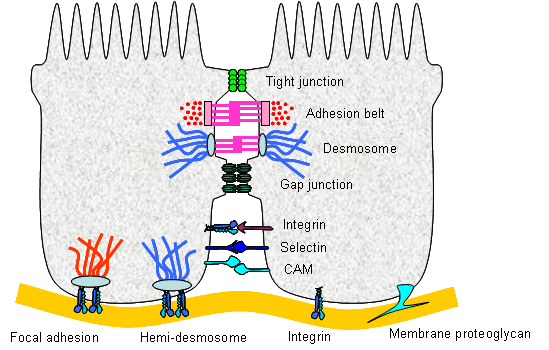
\includegraphics[scale=0.5]{Cell_adhesion_summary.png}
\caption{\label{jonctions} Schéma résumant les différents types de jonctions cellule-cellule ou cellule-matrice.}
\end{figure}

\paragraph{Interactions cellules-cellules}
Les cellules se lient les unes aux autres pour se reconnaître, communiquer et former une structure complète. 

La super famille des immunoglobulines comprend des molécules d'adhésion (IgCAM), souvent spécifiques à un type cellulaire. Elle comprend également les complexes majeurs d'histocompatibilité, qui permettent au système immunitaire de reconnaître les cellules de son propre organisme. 

Les cellules échangent entre elles des espèces chimiques et des signaux électriques. 
Les jonctions communicantes permettent une communication directe entre deux cellules en contact. Les espèces chimiques peuvent passer librement de l'une à l'autre. Cela peut amplifier un signal hormonal, perçu par une cellule et transmis à travers ces jonctions aux voisines qui n'ont pas capté le signal directement. Elles peuvent également servir à transmettre très rapidement un signal électrique. 
Les synapses sont un système très élaboré de communication entre deux cellules par échange d'espèces chimiques (les neurotransmetteurs) par exocytose dans un espace inter-cellulaire réduit. 

Au contraire, les jonctions serrées permettent de créer une étanchéité de part et d'autre d'une monocouche cellulaire. Les cellules épithéliales forment un feuillet continu lié par des jonctions serrées qui maintient la séparation entre le milieu extérieur (la lumière) et le milieu intérieur, par exemple au niveau de la peau, des muqueuses, de l'intérieur du tube digestif\dots

Les cadhérines forment une famille de protéines exprimées partout dans l'organisme à tous les stades de son développement. 
Il existe une trentaine de gènes de cadhérines, et encore plus de protéines exprimées grâce à l'épissage. Ces différentes protéines sont spécifiques selon le type cellulaire.
Les cadhérines de deux cellules voisines peuvent interagir par leur domaine extra-cellulaire pour former une jonction (interaction trans). Les cadhérines peuvent également interagir par leur domaine transmembranaire entre cadhérine d'une même membrane et former des amas (interaction cis)(voir l'article en annexe). 
Les cadhérines permettent de maintenir l'intégrité mécanique d'un tissu de cellules en connectant les cytosquelettes de cellules voisines entre eux. Les cadhérines desmosomales lient les réseaux de filaments intermédiaires, alors que les cadhérines classiques lient les réseaux d'actine (cet aspect sera développé dans le chapitre sur l'actine). 


\paragraph{Interactions cellules-matrice}

La famille des intégrines est le principal médiateur des interactions cellule-substrat. Elles forment des hétérodimères entre une forme alpha et une forme beta. Comme il existe 18 formes alpha et 8 formes beta, au total, les différentes combinaisons entre les unités alpha et beta forment 24 dimères (toutes les combinaisons ne sont pas possibles).  Ces dimères sont exprimés dans différents types cellulaires et qui se lient à différentes protéines de la matrice extra-cellulaire comme le collagène ou la fibronectine. 
Les intégrines relient la matrice extra-cellulaire au cytosquelette d'actine sous la membrane plasmique. Du côté interne de la membrane, l'intégrine se lie à des protéines comme la vinculine, la paxiline, la zyxine, ou la taline pour former des complexes appelés adhésions focales. Plusieurs centaines de protéines ont déjà été impliquées dans les adhésions focales. 
Les intégrines sont la porte d'entrée des signaux mécaniques de la MEC. La plupart des molécules qui s'associent aux intégrines sont impliquées dans la mécanotransduction car elles sont responsables du déclenchement de voies de signalisation en réponse aux signaux reçus par les intégrines. 

\subsection{Cytosquelette}

Le cytosquelette est l'armature sur laquelle repose la cellule pour maintenir sa forme. Il lui permet d'exercer et de sentir des forces, de se déplacer, de gérer l'organisation interne de ses organites et le trafic entre elles. Il est composé de trois réseaux de protéines assemblées en filaments : les microtubules, les filaments intermédiaires et l'actine. 

Les filaments du cytosquelette sont en réorganisation constante : la polymérisation\footnote{Ici, il ne s'agit pas d'une polymérisation au sens chimique. La structure des filaments du cytosquelette est semblable à celle d'un polymère mais à une échelle différente, et les interactions en jeu sont tout à fait différentes. Par analogie, on parle de monomères, de polymérisation et de protéines de pontage.} et la dépolymérisation ont lieu en permanence, à des rythmes qui sont étroitement régulés par la cellule. 
Des protéines de pontage peuvent lier ces filaments pour former un gel réticulé, tandis que d'autres protéines peuvent se lier aux extrêmité pour contrôler la cinétique de polymérisation ou de dépolymérisation. Certaines des protéines de pontage sont des moteurs : elles peuvent convertir de l'énergie chimique en énergie mécanique et mettre le gel de filaments sous tension. 

\subsubsection{Microtubules}

\begin{figure}
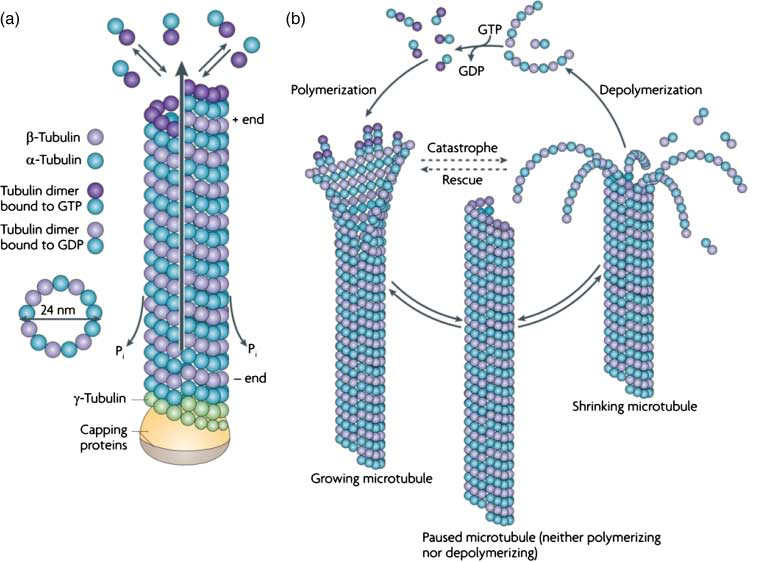
\includegraphics[scale=0.5]{Microtubule.png}
\caption{Construction et destruction des microtubules, d'après \cite{huber_emergent_2013}.}
\end{figure}
La tubuline, composée de deux sous-unités (alpha et bêta), s'associe en protofilaments de treize monomères, qui vont s'associer pour former de longs filaments creux de diamètre 25nm. Ces filaments sont polarisés, une extrémité ne comportant que des sous-unités beta (notée +) et l'autre que des alpha (notée $-$ ), la polymérisation ayant lieu à l'extrémité + et la dépolymérisation à l'extrémité -. 
Le microtubule est le filament le plus rigide du cytosquelette, sa longueur de persistance est de l'ordre du millimètre, bien plus que la taille d'une cellule. 

Dans les cellules eucaryotes, les microtubules sont organisés autour d'un élément central : le centrosome. A partir de cet élément central, les microtubules irradient vers la périphérie cellulaire. 
Sur les microtubules, deux types de moteurs moléculaires se déplacent, les dynéines et les kinésines, respectivement de l'extrémité + vers - et de - vers +.  

Les microtubules organisent les éléments de la cellule et assurent le transport entre les organites, en particulier par le déplacement des vésicules. Les moteurs moléculaires conduisent les vésicules d'un organite à l'autre, par exemple les protéines nouvellement synthétisées vers l'appareil de Golgi, ou les protéines de la matrice extra-cellulaire vers la membrane. 

Les microtubules jouent un rôle prépondérant lors de la mitose. Ils s'assemblent en un fuseau au bout duquel se trouve les centrosomes. Au centre s'alignent les paires de chromosomes, qui sont séparés et emmenés vers les centrosomes. La plupart des drogues perturbant les microtubules bloquent la mitose et sont utilisées pour cette raison dans les traitements anti-cancéreux. 

Par ailleurs, les flagelles et les cils, par exemple le flagelle du spermatozoïde, sont composés d'un faisceau de microtubules animé par les moteurs moléculaires. 

\subsubsection{Filaments intermédiaires}

Contrairement à l'actine et à la tubuline, qui sont conservées et exprimées dans tous les types cellulaires, les filaments intermédiaires sont une famille de protéines dont l'expression dépend du type cellulaire (à l'exception de la lamine). 
Leur assemblage ne nécessite pas non plus l'hydrolyse d'ATP ou de GTP, il est spontané, et il n'existe pas de moteurs moléculaires se déplaçant sur ces filaments. 

Les réseaux de filaments intermédiaires sont liés aux protéines transmembranaires (cadhérines, intégrines) au niveau de structures appelées desmosomes et hémidesmosomes (nom qui vient de la desmine) qui participent à l'intégrité mécanique des tissus. 

Le réseau de filaments intermédiaires est plus stable que les deux autres réseaux du cytosquelette, qui sont en construction et destruction permanentes. Leur rôle est principalement d'ancrer les différents organites dans la cellule. 

Les plus connus des filaments intermédiaires sont sans doute les kératines, exprimées dans les cellules épithéliales et qui sont le constituant principal des poils et des ongles des mammifères (la kératine des reptiles et des oiseaux ne présente pas d'homologie avec celle des mammifères). 

La vimentine est exprimée dans toutes les cellules d'origine mésenchymateuse. Elle joue un rôle dans la localisation des vésicules bien que ne participant pas directement à leur transport, puisqu'on ne connaît pas de moteur moléculaire associé aux filaments intermédiaires  \parencite{styers_intermediate_2005}. Elle est également impliquée dans la régulation de l'adhésion et de la migration cellulaire  (\cite{lynch_endoplasmic_2013},\cite{helfand_vimentin_2011}). 
L'expression de vimentine est souvent un marqueur de la transition épitéhlio-mésenchymateuse. 

Plusieurs types de filaments intermédiaires sont exprimés dans les neurones, et deux types, la filensine et la phakinine, sont spécifiquement responsables de la transparence du cristallin. 

\subsubsection{Les lamines}
\begin{figure}
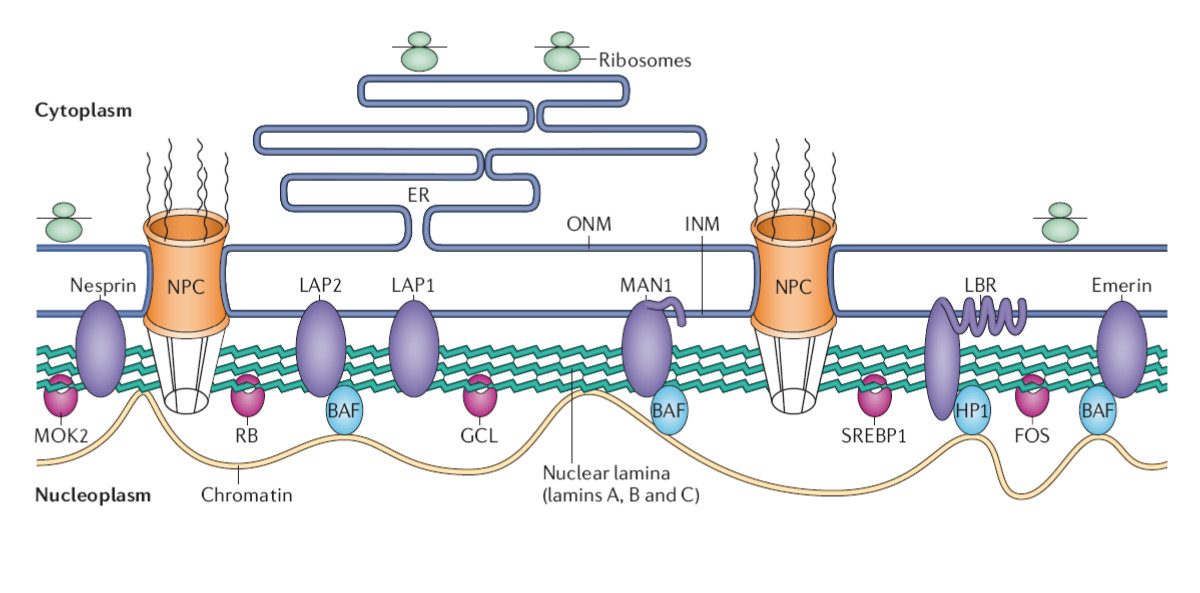
\includegraphics[scale=1.5]{Structure_and_function_of_the_nuclear_lamina.jpg}
\caption{Les lamines (filaments verts) soutiennent l'organisation de la membrane nucléaire (en bleu : ONM Outer Nuclear Membrane, INM Inner Nuclear Membrane). Des protéines comme l'émerine ou la nesprine (ovales violets) sont enchâssées dans l'INM et dans le réseau de lamines, tout comme les pores nucléaires : (NPC Nuclear Pore Complex) qui permettent le traffic nucléo-cytoplasmique. La membrane nucléaire extérieure se replie pour former le Reticulum Endoplasmique (ER), siège de la traduction de l'ARN en protéine par les ribosomes (en vert). Le réseau de lamines est également relié à la chromatine à l'intérieur du noyau.  . Illustration par  \cite{coutinho_molecular_2009} \label{membrane nucléaire}}
\end{figure}
Les lamines diffèrent des autres filaments intermédiaires sur plusieurs points. Elles ne forment pas un réseau dans toute la cellule mais sont localisées à la membrane nucléaire, et elles sont exprimées dans tous les types cellulaires. 

Les lamines forment un réseau soutenant la membrane nucléaire interne, dans laquelle sont ancrés les pores nucléaires (figure \ref{membrane nucléaire}). Par l'intermédiaire de protéines comme la nesprine, le réseau laminaire est couplé mécaniquement au cytosquelette d'actine de la cellule et il est couplé à l'actine nucléaire par l'émerine, protéine qui coiffe la pointe des filaments d'actine et augmente leur polymérisation. 
Le réseau de lamines est nécessaire au maintien de l'intégrité du noyau et définit ses propriétés mécaniques. 
Les lamines organisent également la chromatine à l'intérieur du noyau et contribuent à réguler l'expression du génome (\cite{dechat_nuclear_2008}).

La progéria est liée à des mutations sur le gène de la lamine A  et le syndrôme de dystrophie musculaire d'Emery-Dreifuss à des mutations de l'émerine. 


\subsubsection{Filaments intermédiaires dans les cellules musculaires}
\begin{figure}
\includegraphics[scale=0.15]{sarcomere.png}
\caption{Schéma de l'organisation d'un sarcomère. On peut voir les filaments de desmine (en gris) s'enrouler autour de la structure formée par les filaments d'actine (en rouge) au niveau du disque Z. Toute cette structure est décrite en détail au chapitre 4.  }
\end{figure}
Quatre types de filaments intermédiaires sont exprimés dans la cellule musculaire : la desmine, la vimentine, la lamine et la synésine. 
La desmine et la vimentine ont des structures suffisamment proches pour pouvoir former des hétéro-dimères et s'associer dans des filaments. La synésine ne peut former que des hétéro-dimères avec les autres filaments intermédiaires. 

La desmine, la vimentine et la synésine ont un rôle dans l'organisation des fibres musculaires qui sera développé dans le chapitre consacré au muscle. 



\subsubsection{Actine}
  
L'actine constitue le réseau du cytosquelette le plus versatile et le plus dynamique. Son réseau est constamment réorganisé, et elle est le composant essentiel de la motilité cellulaire. 

Toutes les cellules eucaryotes expriment des actines, qui sont hautement conservées de la levure jusqu'à l'humain. Ce sont également des protéines très exprimées, et l'actine peut représenter jusqu'à 15\% de la masse de protéines dans une cellule (\cite{alberts_molecular_2002}).

La membrane plasmique est une bicouche lipide qui a de faibles modules élastiques. Un réseau dense et très branché d'actine forme une couche rigide sous la membrane et confère sa forme à la cellule : le cortex d'actine. Ses propriétés sont essentielles dans les déformations des cellules et dans leur interaction avec un substrat. 
Dans le volume de la cellule, l'actine forme un réseau moins dense. \textit{In vitro} on peut observer des faisceaux de filaments appelés fibres de stress. 
Dans le muscle, l'actine et ses moteurs associés (les myosines) forment une organisation spécialisée responsable de la contraction musculaire, appelée sarcomère, qui sera décrite dans le chapitre dédié au muscle.

L'actine interagit avec un très grand nombre de protéines, ce qui confère au réseau un caractère particulièrement dynamique. L'actine n'est pas limitée à un rôle mécanique, elle a également des rôles de régulation de l'expression du génome et d'organisation de l'ADN. 

Le couplage entre le rôle mécanique de l'actine et son rôle transcriptionnel est au c\oe ur de ce travail de thèse, c'est pourquoi l'actine sera présentée en détail dans le chapitre suivant. 




\section{Expression du génome}

Le génome d'un organisme contient toute l'information nécessaire à la reconstitution de l'organisme entier. Cependant, il est évident dans un organisme pluricellulaire que si toutes les cellules contiennent le même génome, elles ne l'expriment pas de la même manière. C'est également le cas chez des êtres unicellulaires : des bactéries ou des levures ayant le même génome ne vont pas l'exprimer de la même manière selon les conditions extérieures. 

Les parties codant directement pour des protéines ne représentent qu'une toute petite partie de l'ADN. Autour des séquences codantes, le reste du génome aide à déterminer quelles protéines doivent être synthétisées, et dans quelles quantités. 

\subsection{Des gènes aux protéines}

Le chemin d'un gène à une protéine fonctionnelle passe par trois étapes principales : la transcription de l'ADN en ARN, la maturation de l'ARN et la traduction de l'ARN en protéine.

\subsubsection{La transcription}

L'information génétique est stockée dans l'ADN, pour y être protégée et transmise d'une génération à l'autre. Les quatre bases de l'ADN fonctionnent par paires, et grâce à ce mécanisme un brin d'ADN peut être complété par sa séquence miroir. 

Lorsque toutes les conditions d'expression sont réunies, l'ARN polymérase peut se fixer sur l'ADN au site de début de transcription. Le complexe ouvre l'ADN, et permet aux bases de l'ARN, Adénine, Uracile, Guanine et Cytosine, de compléter les bases de l'ADN, respectivement Thymosine, Adénine, Cytosine et Guanine. L'ARN polymérase progresse ainsi jusqu'à rencontrer une séquence de terminaison sur l'ADN. 

À l'issue de cette étape, un ARN a été transcrit directement à partir de la séquence codante. 

\subsubsection{La maturation de l'ARN}

Après sa transcription, l'ARN subit plusieurs transformations. Des éléments sont ajoutés à ses deux extrémités, pour assurer sa stabilité et sa reconnaissance par les ribosomes. 
L'ARN transcrit comprend deux types de séquences, les introns et les exons. Seuls les exons contiennent l'information des acides aminés pour coder la protéine. 
L'ARN va subir une étape d'épissage : les introns sont retirés de l'ARN jusqu'à ce qu'il ne reste que l'enchaînement des exons. Lors de cette étape, tous les exons peuvent être réassemblés, ou seulement une partie d'entre eux. Les protéines synthétisées par ces reconstitutions différentes seront différentes : on parle d'épissage alternatif. 
Un même gène peut donc coder pour des protéines différentes grâce au jeu de l'épissage. Par exemple, il existe chez la drosophile un unique gène qui peut coder pour plus de 38 000 protéines différentes (\cite{schmucker_drosophila_2000}), ce qui est du même ordre de grandeur que le nombre total de gènes dans le génome de la drosophile. 

Après sa maturation, l'ARN messager est exporté du noyau pour se diriger vers le réticulum endoplasmique.

Tous les ARN n'ont pas vocation à être traduits en protéines : certains vont accomplir leur fonction sous cette forme. C'est le cas des éléments de la machine de traduction (ARN de transfert et ARN du ribosome), ou des micro-ARN, qui vont participer à la régulation de l'expression des gènes en aval de la transcription.

Une des techniques utilisées pour supprimer l'expression d'un gène est de bloquer l'ARNm produit par la transcription de ce gène avec un ARN qui va le compléter paire à paire pour former un double brin (siRNA). Cela empêche alors sa traduction en protéine. 

\subsubsection{La traduction}

Le code génétique est la correspondance entre des triplets de nucléotides, les codons, et les acides aminés qui composent les protéines. 

La traduction commence au codon start le plus proche du début de l'ARN messager. La plupart du temps, chez les eucaryotes, il s'agit d'un triplet AUG, codant pour une Méthionine, cependant on découvre de plus en plus de séquences qui commencent avec un codon start alternatif. C'est le cas par exemple de la protéine Myocardin-Related Transcription Factor A, qui a deux variants d'épissage, l'un débutant par un codon GTG (Valine) (\cite{scharenberg_tgf-_2014}).

Le travail de traduction est assuré par le ribosome, un assemblage complexe de protéines et d'ARN et par des ARN de transfert. Les ARN de transferts sont l'assemblage d'un ARN replié en croix et d'un acide aminé. À une extrémité, l'ARN présente un triplet anti-codon, le complémentaire d'un codon du code génétique. À l'autre se trouve l'acide-aminé correspondant à ce codon. 

Au début de la traduction, le ribosome se fixe sur le codon start, puis, il va chercher un ARN de transfert dont le triplet anti-codon corresponde au premier triplet sur la séquence à traduire. Comme quelqu'un qui teste différentes clés pour ouvrir une serrure, le ribosome va chercher l'ARN de transfert qui lui permet de faire correspondre un acide aminé à un codon. Lorsqu'il l'a trouvé, il attache l'acide aminé au précédent de la séquence, et ainsi de suite jusqu'à arriver à un codon stop. 

On parle souvent \emph{du} code génétique, car il est commun à un grand nombre d'êtres vivants, mais il en existe des variantes apparues au cours de l'évolution. En particulier, dans les cellules eucaryotes, l'ADN des mitochondries utilise un autre code génétique que celui de l'ADN de la cellule elle-même. 

\subsubsection{Modifications post-traductionnelles}

Les protéines commencent à se replier dès le début de leur synthèse par le ribosome. Mais certaines requièrent l'aide d'autres protéines, appelées chaperons, pour arriver au repliement correct. D'autres encore nécessitent des modifications chimiques après la traduction. 

Tous les acides aminés peuvent faire l'objet de modifications post-traductionnelles. La plus connue est sans doute la phosphorylation, ajout d'un groupe phosphate à un acide aminé par des enzymes, les kinases. La phosphorylation joue le rôle de bouton on/off pour un grand nombre de protéines dans des voies de signalisation. Ce sera le cas des voies de signalisation qui seront présentées au chapitre 3, faisant intervenir les kinases ROCK, LIMK ou ERK1/2. 
Autre exemple de modification, l'oxydation de l'actine sera également évoquée au chapitre 2. 


\subsection{Régulation de l'expression du génome}

\subsubsection{Réorganisation de la chromatine}

L'ADN est stocké dans la cellule sous une forme condensée, la chromatine. Selon leur état biochimique (acétylation, méthylation) les histones forment un enroulement plus ou moins compact de l'ADN. Par exemple, chez les femelles mammifères, l'un des deux chromosomes X est désactivé afin de ne pas avoir deux fois plus de transcription des gènes portés par ce chromosome qu'un organisme mâle. Il est condensé définitivement sous forme d'hétérochromatine. 

La compaction de l'ADN dans l'hétérochromatine ou dans l'euchromatine détermine donc quels gènes sont accessibles pour être transcrits et quels gènes sont désactivés dans l'hétérochromatine. 
La régulation de cette organisation par la modification chimique des histones est donc la première étape de la régulation transcriptionnelle du génome. 

\subsubsection{Les facteurs de transcription}

L'ARN polymérase ne peut pas se lier seule de manière stable sur l'ADN pour initier la transcription. 
Les facteurs de transcription forment une famille de protéines qui ont pour rôle de se fixer sur l'ADN en amont de la séquence à transcrire pour contribuer à l'expression du gène ou au contraire pour la réprimer. 

Un facteur de transcription reconnaît une séquence spécifique sur l'ADN en amont du gène régulé, le promoteur. Les promoteurs en amont d'un gène vont déterminer quels facteurs de transcription vont être capables d'activer la transcription. Des gènes partageant le même promoteur vont être activés par les mêmes facteurs de transcription et répondre aux mêmes stimuli.  

Dans le développement des êtres pluricellulaires, la différenciation des cellules souches totipotentes de l'embryon en différents types de tissus va être orchestrée par l'activation de nombreux facteurs de transcription. 

Les facteurs de transcription vont également être impliqués dans les réponses d'une cellule ou d'un organisme à des signaux biochimiques (hormones, facteurs de croissances, inflammation, poisons, toxines \dots) provenant de cellules voisines (par l'intermédiaire des liaisons transmembranaires entre deux cellules, par une structure spécialisée comme une synapse ou sécrété dans le milieu extra-cellulaire par les cellules voisines) ou des tissus éloignés (hormones circulant dans le corps), mais aussi à des signaux environnementaux comme la température, le choc osmotique, les contraintes mécaniques, l'exposition à la lumière du soleil  \dots

Les facteurs de transcriptions se lient directement à l'ADN, ils doivent donc être présents dans le noyau pour accomplir leur fonction. Certains facteurs de transcriptions sont ainsi régulés par leur localisation : lorsqu'ils sont confinés hors du noyau, ils ne peuvent pas être actifs. C'est le cas du récepteur des \oe{}strogènes, qui est présent dans le cytoplasme en l'absence d'hormones et va être transporté dans le noyau lorsqu'il sera lié aux \oe{}strogènes.

Un facteur de transcription peut recruter d'autres protéines, comme des coactivateurs (ou des corépresseurs) qui vont amplifier (ou diminuer) l'activation de la transcription. Ces cofacteurs peuvent alors eux-mêmes réguler l'activité transcriptionnelle par leur activité (en particulier leur état de phosphorylation) ou par leur localisation. C'est le cas du mécanisme de régulation de Serum Response Factor, qui sera détaillé dans le chapitre 3. 

Un facteur de transcription peut également recruter des protéines qui vont changer localement l'état de compacité de la chromatine, afin de rendre le gène plus facilement ou plus difficilement accessible. 



%\end{document}


%\documentclass{report}
%\usepackage[T1]{fontenc}
%\usepackage[utf8]{inputenc}
%\usepackage[francais]{babel}
%\usepackage{amsmath}
%\usepackage{graphicx}
%\graphicspath{{Figures/}}
%\usepackage[backend=biber,style=authoryear,bibencoding=utf8]{biblatex}
%
%\usepackage[colorlinks,linkcolor=blue]{hyperref}
%
%
%\addbibresource{biblio2.bib}
%
%\begin{document}
\chapter{L'actine}
\begin{center}
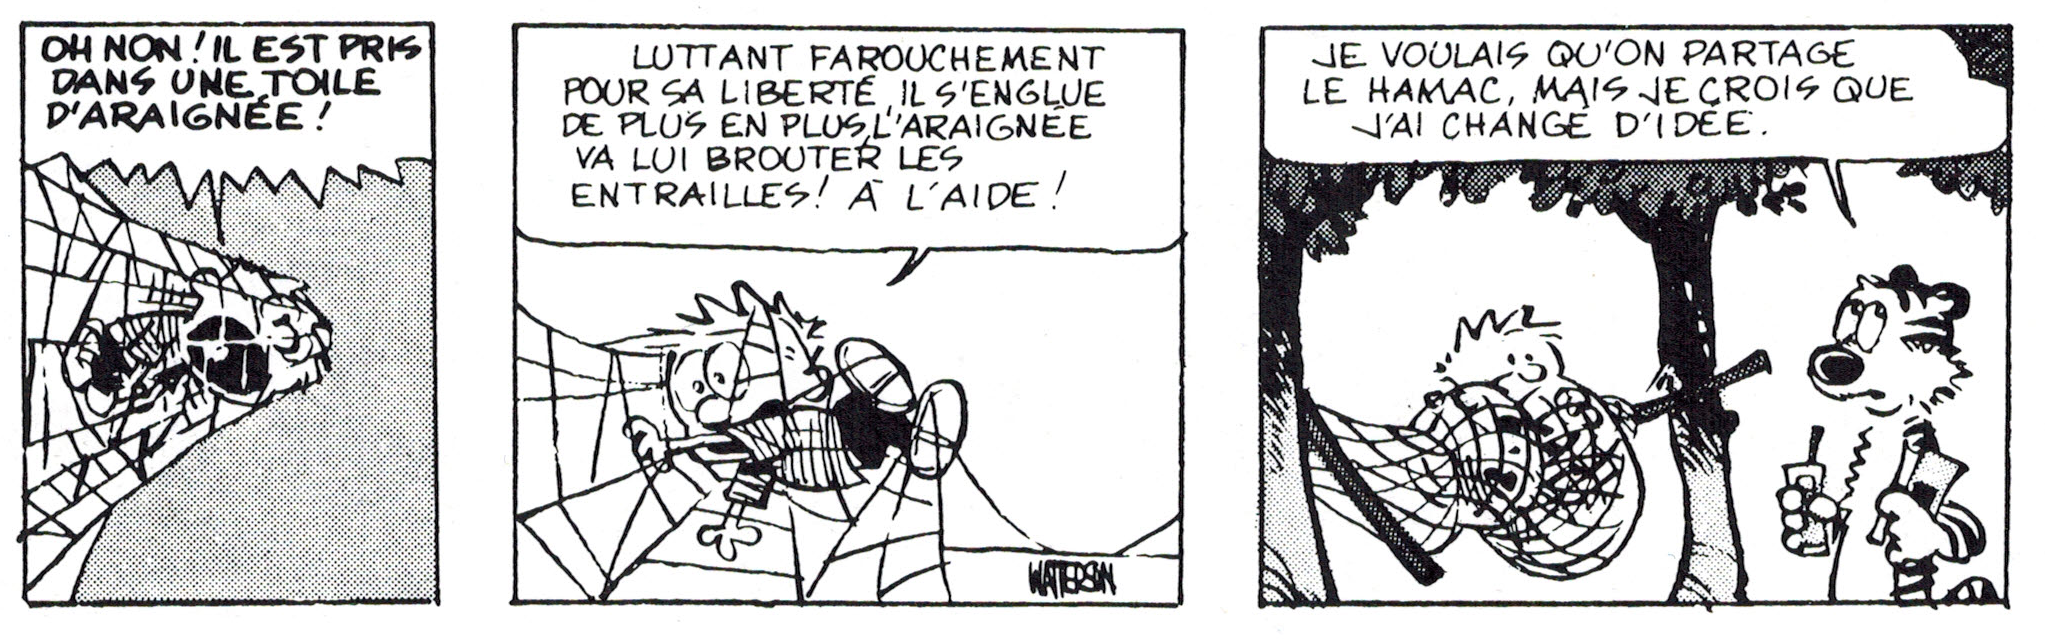
\includegraphics[scale=0.7]{Chapitre2.png}

\end{center}
\newpage
L'actine est une protéine ubiquitaire conservée chez tous les eucaryotes, exprimée dans tous les types cellulaires. 
Ses fonctions sont multiples et variées et se divisent en deux catégories principales, les fonctions mécaniques et les fonctions régulatrices. 

Elle se présente dans la cellule sous deux formes principales : en monomères (actine G pour globulaire) ou en filaments (actine F). 
Elle interagit avec un grand nombre de protéines appelées Actin-Binding Proteins. 

L'actine est un composant du cytosquelette prenant la forme d'un réseau de filaments très dynamique. La rigidité d'une cellule et sa motilité sont majoritairement contrôlées par l'organisation du cytosquelette d'actine. 

Mais l'actine est également un composant des trois ARN Polymérases PolI, PolII et PolIII, qui transcrivent l'ADN en ARN pendant la première étape de l'expression du génome ( \cite{ye_nuclear_2008}, \cite{hofmann_actin_2004} \cite{hu_role_2004}). 
Elle est indispensable à la réorganisation de la chromatine qui précède l'expression (revue par \cite{farrants_chromatin_2008}) mais aussi à l'export de l'ARN (\cite{hofmann_cofactor_2001}).  

L'association de ces rôles mécaniques et biologiques fait de l'actine un acteur de choix dans l'interface entre les signaux mécaniques et les signaux biologiques. 

Dans le corps, l'actine a des fonctions spécifiques dans un grand nombre d'organes, comme la contraction des muscles, l'organisation des dendrites et des axones des neurones, le fonctionnement des plaquettes ou de l'appareil auditif. 



\section{Actine G}

\begin{figure}
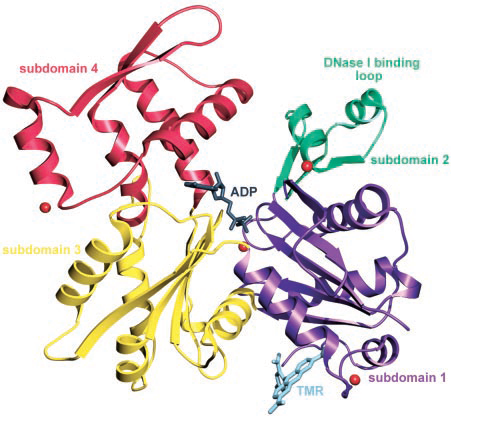
\includegraphics[scale=0.7]{Actine_dominguez.png}
\caption{Monomère d'actine ADP, d'après \cite{otterbein_crystal_2001}}
\end{figure}

Chez les mammifères, l'actine est codée par 6 gènes qui peuvent donner une trentaine de molécules différentes par le jeu de l'épissage. 
Elles sont divisées en trois familles : les actines $\alpha$ qui sont exprimées dans les muscles cardiaques, lisses et squelettiques, les actines $\beta$ et $\gamma$ exprimées dans tous les types cellulaires.
Les différentes formes d'actine sont très proches en séquence, mais ne peuvent pas complètement se substituer les unes aux autres. Toutes les formes peuvent s'incorporer dans les filaments. 

La protéine transcrite a un poids moléculaire de 42 kDa, et est produite en grande quantité dans les cellules, où elle pèse environ pour 1 à 5 \% de la masse protéique, mais cela peut aller jusqu'à 15\% de la masse d'une cellule musculaire. 

\subsection{Structure}
La structure moléculaire de l'actine a été observée un grand nombre de fois, en cristallisation avec différents ABP comme la Dnase, la latrunculine ou la profiline. 

Elle est composée de 4 sous-domaines organisés en deux lobes. Les sous-domaines 2 et 4 forment l'extrémité $-$ du filament, les sous-domaines 1 et 3 forment l'extrémité +. Entre les deux lobes se trouve le site de liaison à l'ATP. 
À côté de ce site se trouve une zone d'interaction avec les cations divalents (Ca$^{2+}$ ou Mg$^{2+}$). 

Dans le sous-domaine 2 se trouve une structure de 8 acides aminés appelée Dnase binding loop, désorganisée dans la plupart des cristallisations de l'actine mais organisée en feuillet $\beta$ lorsqu'elle est liée à la DNase. Au centre de cet élément se trouve une méthionine en position 44 qui peut être oxydée par la protéine MICAL, dont je reparlerai plus en détail plus loin dans ce chapitre et dans le chapitre suivant. 

\subsection{L'actine est une ATPase}

L'actine, après sa fabrication, n'est prête à jouer son rôle qu'avec l'ajout d'une ATP au centre de sa structure.
En plus de ses deux formes, globulaire ou filamenteuse, l'actine est capable d'hydrolyser l'ATP en ADP.

Les deux formes d'actine, ATP et ADP sont capables de former des filaments et de s'incorporer à des filaments. 


\subsection{Localisation et transport}

L'actine a longtemps été étudiée pour son rôle dans le cytoplasme, en tant que composant du cytosquelette. Cependant de l'actine est également présente dans le noyau de la cellule, où elle a des rôles essentiels. 
L'actine peut polymériser dans les deux compartiments (\cite{mcdonald_nucleoplasmic_2006},\cite{baarlink_nuclear_2013}), bien que l'on ne trouve pas de grands filaments organisés dans le noyau. 

L'actine est à une taille intermédiaire pour les pores nucléaires : elle n'est pas tout à fait assez petite pour diffuser facilement à travers. Elle est donc transportée activement entre le noyau et le cytoplasme. 
Son import nécessite la liaison à la cofiline, et est médiée par l'importine 9 (\cite{dopie_active_2012}). Son export nécessite la profiline et est médiée par l'exportine 6 (\cite{dopie_active_2012}).



\subsection{Oxydation de l'actine}

Les protéines MICAL sont capables d'ajouter deux atomes d'oxygène sur la Méthionine qui se trouve en 44e position de la la chaîne d'acides aminés de l'actine. Cet acide aminé est au centre d'une zone de la protéine qui relie les monomères dans un filament. 
L'oxydation spécifique de cet acide aminé déstabilise les filaments et l'actine oxydée est incapable de se lier à d'autres actines pour former de nouveaux filaments (\cite{hung_direct_2011}). 



\subsection{Protéines interagissant avec l'actine G}

 La profiline est une petite protéine (autour de 15kDa) qui peut se lier à l'extrémité + de l'actine G, l'empêchant de former un nouveau filament ou de se lier à l'extrémité $-$ d'un filament existant. 
Bien qu'elle se lie au monomère, son action est globalement favorable à la croissance des filaments (\cite{pollard_quantitative_1984}). 
La profiline facilite le remplacement d'une ADP par une ATP dans le monomère auquel elle est attachée. 
Or l'actine ATP polymérise mieux que l'actine ADP, l'action de la profiline va donc recycler l'actine ADP dépolymérisée des anciens filaments en actine ATP prête à allonger de nouveaux filaments. 
De plus, les élongateurs de filaments comme les formines et VASP vont préférentiellement utiliser de l'actine liée à la profiline pour faire croître les filaments (\cite{ferron_structural_2007},\cite{romero_formin_2004}). 
La profiline joue également un rôle dans la localisation de l'actine : l'exportine 6 va se lier spécifiquement au complexe actine-profiline et le faire passer de l'intérieur vers l'extérieur du noyau (\cite{dopie_active_2012}).


Les thymosines $\beta 4$ sont de toutes petites protéines d'environ 5kDa dont le rôle principal est de maintenir un réservoir d'actine monomérique \parencite{safer_isolation_1990}. Elles se lient principalement aux actines ATP et les empêchent de polymériser. 

Les CAP (Adenylate Cyclase Associated Protein) sont également des catalyseurs de l'échange d'un ADP contre un ATP dans les monomères d'actine (\cite{makkonen_mammalian_2013}). 

Les cofilines sont une famille de petites protéines qui lient à l'actine G et à l'actine F. Elles ont une préférence pour l'actine ADP. 
Le complexe cofiline-actine est plus facilement recruté par les CAP, qui vont  dissocier le complexe et remplacer l'ADP par une ATP sur l'actine. 
Les cofilines sont suffisamment petites pour passer par les pores nucléaires par diffusion, elles sont cependant dotées d'un signal de localisation nucléaire. Cela leur permet d'être importées dans le noyau lorsqu'elles sont liées à d'autres protéines plus massives. 
Ainsi, le complexe cofiline-actine est importé dans le noyau par l'importine 9 (\cite{dopie_active_2012}).

L'actine bloque l'activité de la DNase I, une enzyme qui coupe l'ADN en fragments de 4 paires de bases de manière non spécifique. La DNase I se lie à l'actine globulaire avec une grande affinité, alors qu'elle ne se lie que très peu à l'actine F, c'est pourquoi elle est souvent utilisée pour la détection de l'actine G en immunofluorescence. 

Les Myocardin-Related Transcription Factors sont des cofacteurs de transcriptions qui peuvent former un complexes avec trois ou cinq monomères d'actine (\cite{mouilleron_molecular_2008}). Leur rôle n'est pas de réguler l'équilibre dynamique de l'actine mais d'agir comme un détecteur de la concentration de monomères d'actine disponibles. 
En fonction de l'état de polymérisation du cytosquelette, les MRTF vont réguler l'activité de Serum Response Factor, un facteur de transcription contrôlant les gènes de l'actine et d'un grand nombre d'ABP qui régulent sa dynamique. 
Les MRTF sont un maillon d'une boucle de rétro-action qui contrôle la dynamique de l'actine à long terme par l'expression des gènes (\cite{salvany_core_2014}). 
Les mécanismes détaillés de ce contrôle et ses conséquences seront décrits dans le chapitre 3. 

\begin{figure}
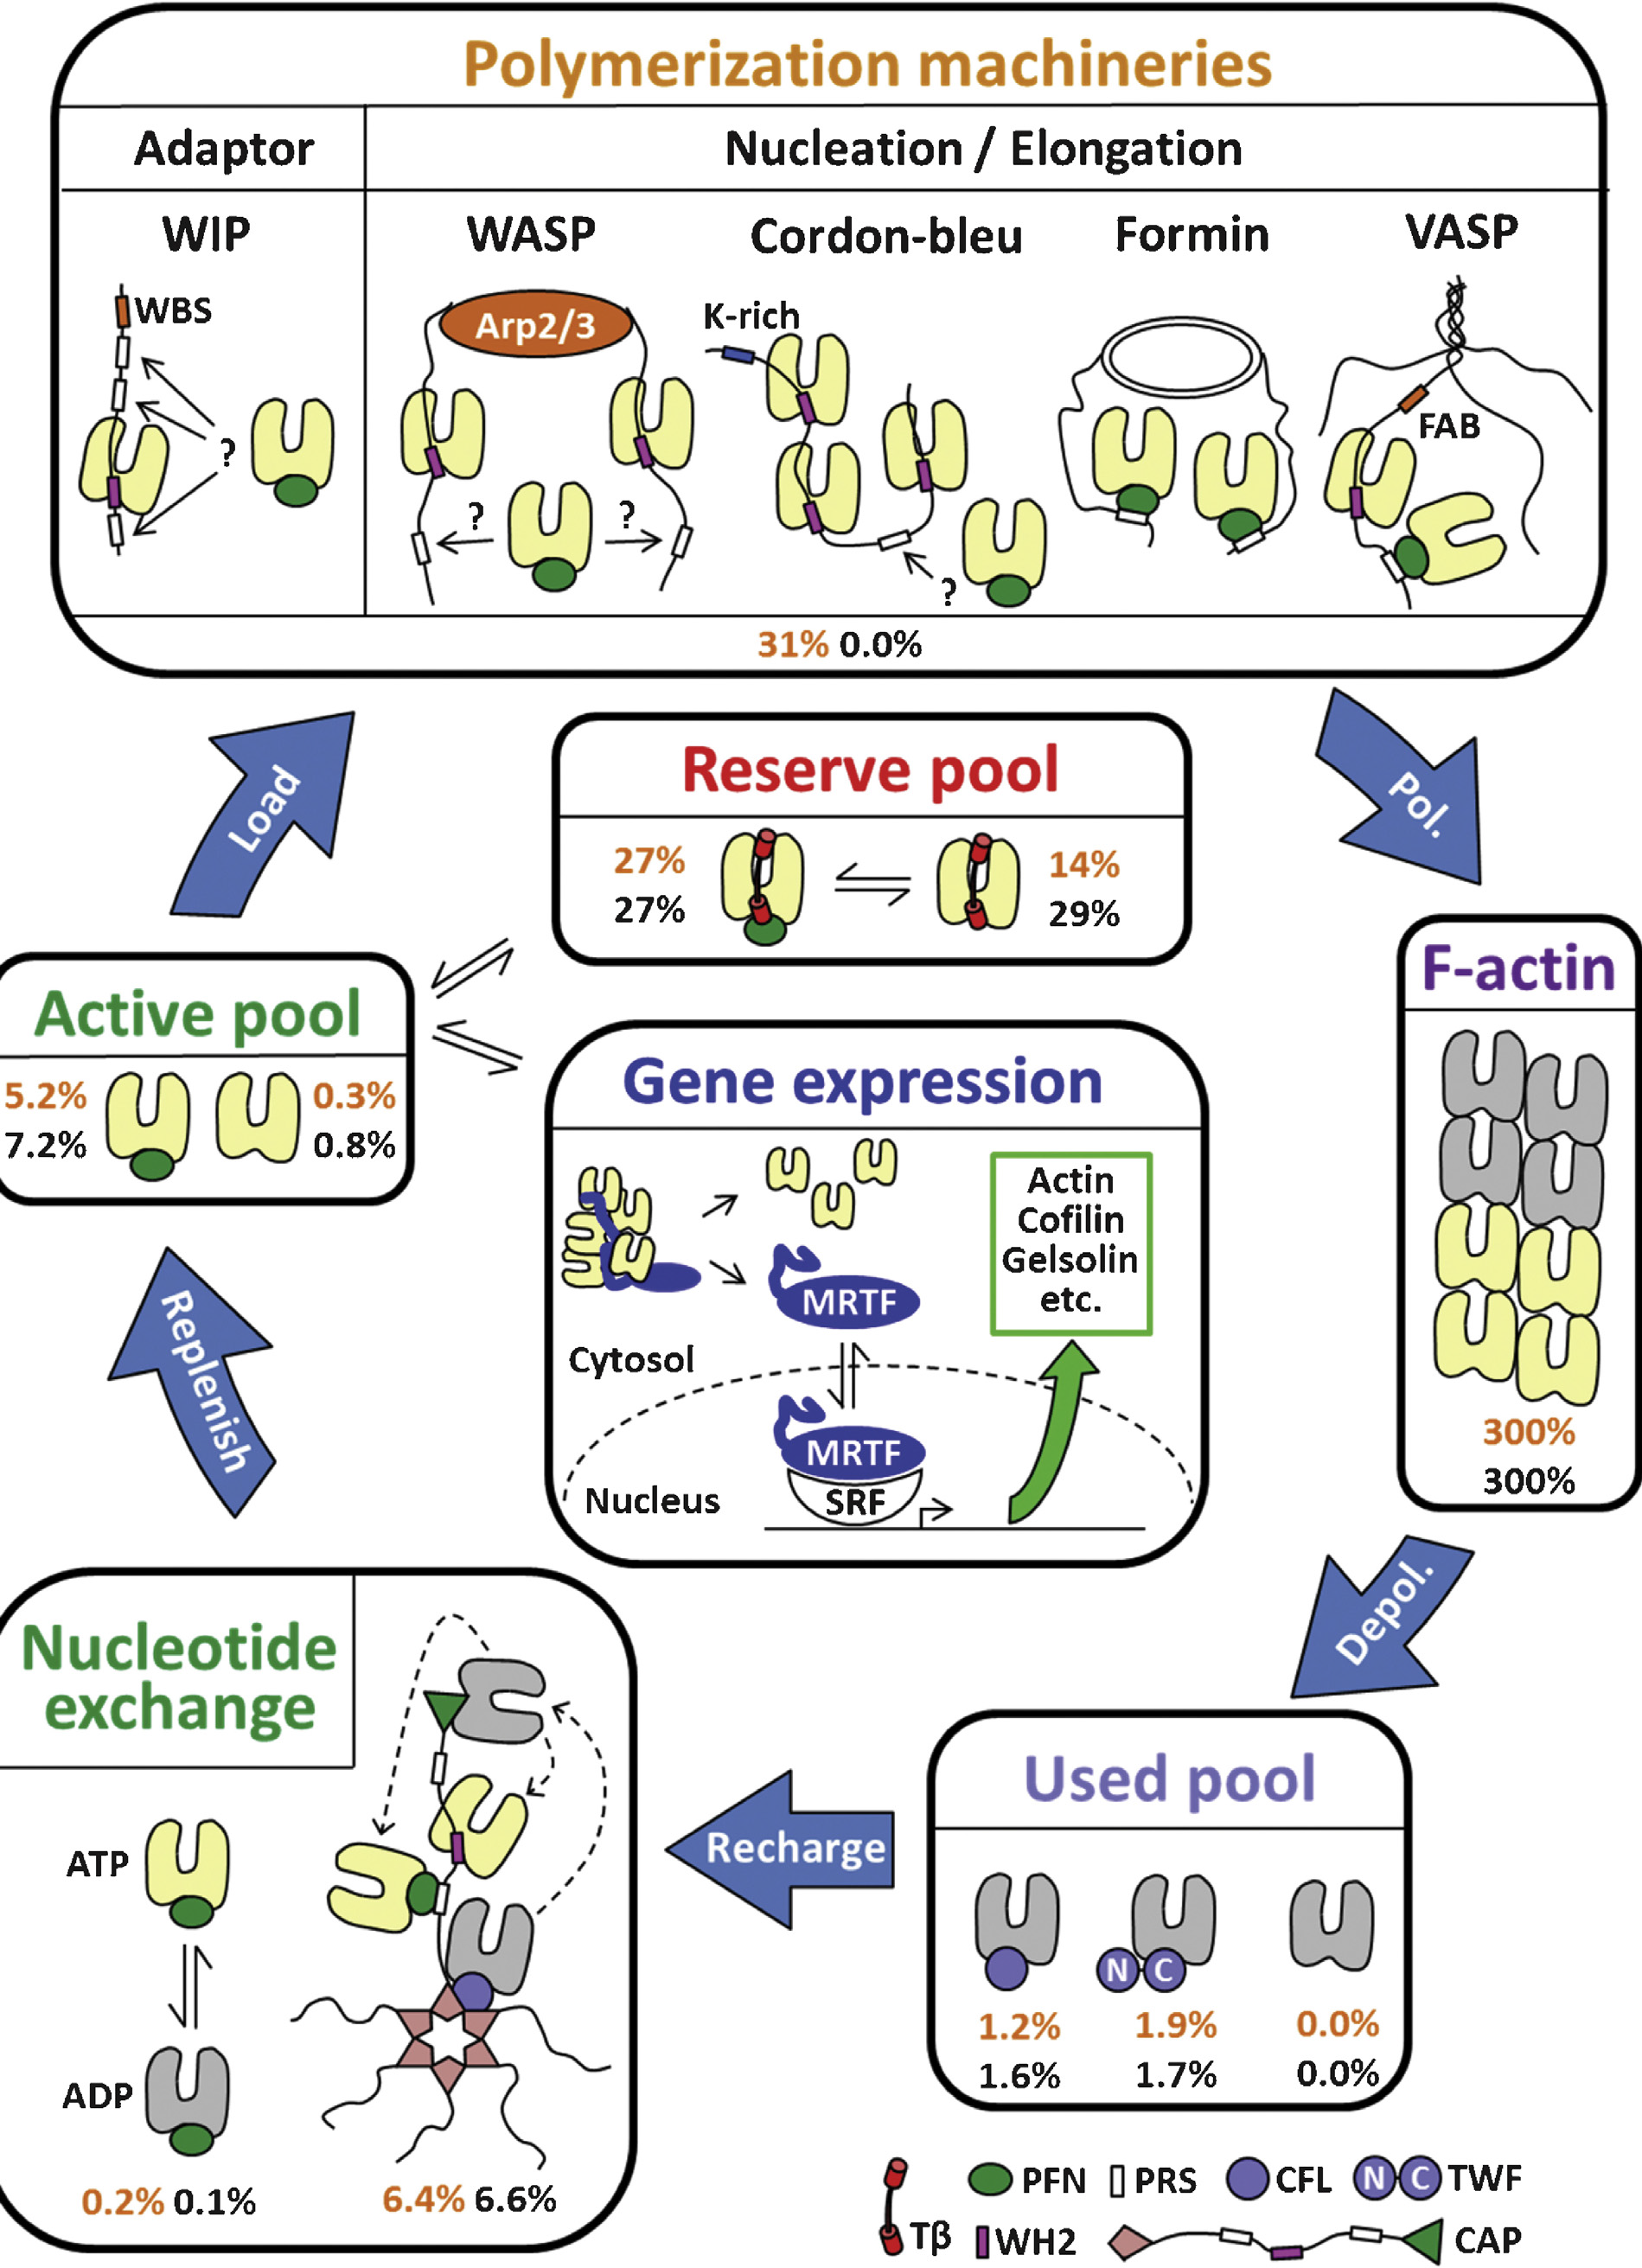
\includegraphics[scale=0.25]{actine_cycle.png}
\caption{Cycle de polymérisation et dépolymérisation de l'actine dans la cellule sous l'effet des différentes protéines liées à l'actine, d'après la revue de \cite{xue_guardians_2013}. PFN : profiline, PRS : proline rich sequence, CFL : cofiline, TWF : twinfiline, WH2 : Wiskott-Aldrich syndrome homology region 2, T$\beta$ : thymosine $\beta$. } 
\end{figure}

\section{Actine F}

La principale fonction de l'actine chez les eucaryotes est sa capacité à former un réseau de filaments branchés, connecté par des moteurs moléculaires. 
La formation de filaments d'actine est régulée par de très nombreuses protéines qui vont se lier aux monomères ou aux filaments. 

\begin{figure}
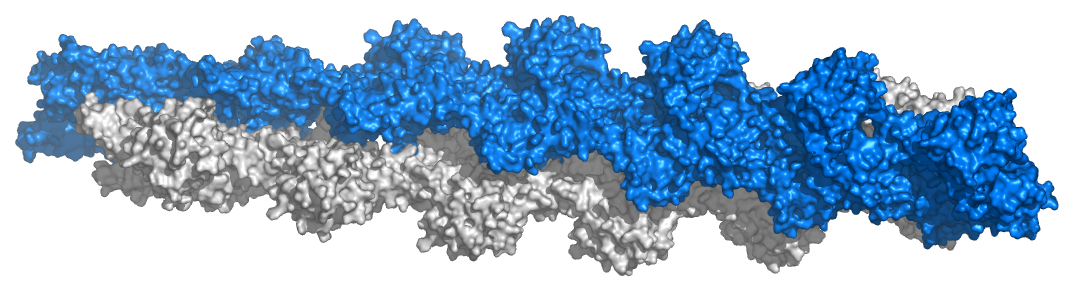
\includegraphics[scale=0.3]{Actin_filament_atomic_model.png}
\caption{Structure d'un filament d'actine basée sur le modèle de \cite{holmes_atomic_1990}, illustré par Thomas Splettstoesser}
\end{figure}

\subsection{Le filament}

Les filaments d'actine sont très dynamiques, et ont une structure changeante. Ils ont un diamètre de 6nm et une longueur de persistance de l'ordre de la dizaine de microns, donc du même ordre de grandeur que la taille typique cellulaire. 

Les monomères d'actine s'associent les uns à la suite des autres, l'extrémité $-$ d'un monomère se liant à l'extrémité + de l'autre, avec une rotation entre un monomère et l'autre. 
Le filament est alors polarisé, avec une extrémité $-$ appelée également pointue et une extrémité + appelée barbée. 

L'actine ATP est plus facilement polymérisée alors que l'actine ADP est plus facilement dépolymérisée. 
Les actines ATP incorporés dans un filament sont ensuite hydrolysées, et deviennent donc plus facilement dépolymérisables.
Les deux bouts du filament ont alors des affinités différentes pour les monomères. En présence d'une grande quantité de monomères disponibles, le filament peut croître par les deux bouts, mais dans une concentration intermédiaire, le filament va croître par ajout de monomères à son extrémité + et décroître par dépolymérisation à l'extrémité $-$. L'équilibre entre les deux cinétiques de réaction détermine si la taille du filament croît ou non. 

Cet équilibre est connu comme le \og tapis roulant \fg de l'actine : lorsque les deux cinétiques sont égales, le filament avance par remplacement des monomères en gardant une longueur constante. 

Bien que cet assemblage puisse avoir lieu spontanément en présence d'actine, de nombreuses protéines aident à la nucléation des filaments, à leur stabilité ou à leur déstabilisation. 

\subsection{L'équilibre de polymérisation}

Des protéines vont réguler toute l'existence d'un filament d'actine : la nucléation, la croissance, la stabilisation et la dissociation. 

\subsubsection{Les nucléateurs}
Les dimères et les trimères d'actine sont des structures peu stables, à la durée de vie assez courte. C'est à partir du tétramère que la structure devient suffisamment stable pour créer un nouveau filament d'actine. 

Afin de dépasser cette barrière, d'autres protéines jouent le rôle de nucléateurs. Le complexe Arp2/3 (Arp pour Actin Related Protein) est le plus connu de ces nucléateurs. Il se lie au côté d'un filament et Arp2 et Arp3 miment un dimère d'actine. D'autres monomères peuvent alors se fixer sur cette base et un nouveau filament peut croître. Ce nouveau filament est de plus attaché avec un angle d'environ 70 \degres au filament initial, créant un réseau branché (\cite{blanchoin_direct_2000}). 

Les formines se fixent à l'extrémité barbée d'un filament et y ajoutent successivement des monomères d'actine. Les formines peuvent nucléer un nouveau filament en stabilisant un dimère et en y ajoutant d'autres monomères(\cite{pring_mechanism_2003}). 

\subsubsection{Les élongateurs}

Une fois les filaments formés, des facteurs d'élongation comme les formines ou Ena/VASP, peuvent ajouter des monomères liés à la profiline à l'extrémité barbée du filament. 
Certaines formines avancent le long du filament tout en le construisant à partir de complexes actine-profiline (\cite{otomo_structural_2005}). 


\subsubsection{Protéines de coiffage (capping proteins)}

Il existe deux sortes de protéines de coiffage : celles qui se lient à l'extrémité barbée et contribuent donc à réduire la polymérisation (comme CapZ, la gelsoline ou la tensine), et celles qui se lient à l'extrémité pointue, empêchant la dépolymérisation (comme la tropomoduline). 


\subsubsection{Protéines de fragmentation (severing proteins)}
Les protéines de fragmentation découpent et dépolymérisent les filaments d'actine. 

La cofiline se lie aux filaments d'actine ADP et entraîne une configuration où la rotation des monomères les uns par rapport aux autres est plus grande (\cite{mcgough_cofilin_1997}). Cela déstabilise les filaments et les casse. 

La gelsoline, la famille des villines et la fragmine sont également des facteurs de dépolymérisation des filaments d'actine. 

À première vue, on peut voir l'impression que ces protéines vont avoir tendance à diminuer le nombre et la longueur des filaments et participer à la destruction du cytosquelette. Cela peut être le cas, mais pas toujours : la fragmentation d'un long filament en de nombreux filaments courts fait apparaître de nombreuses extrémités barbées là où il n'y en avait qu'une seule. Selon les conditions, en particulier l'activation de facteurs d'élongation et la disponibilité des monomères, la fragmentation peut donc agir en faveur de la polymérisation, en particulier lors du remplacement d'un réseau à longs filaments par un réseau très dense et réticulé. 

Les protéines MICAL forment une famille de protéines dépolymérisant l'actine, découvertes récemment dans les neurones (\cite{hung_direct_2011}). En oxydant l'actine des filaments, elle les dépolymérise. Comme l'actine oxydée ne peut plus former de nouveaux filaments, la destruction du cytosquelette par MICAL ne peut pas promouvoir la croissance du réseau. 

MICAL2 est un membre de la famille des protéines MICAL qui est particulièrement localisé dans le noyau. L'actine qu'elle oxyde, en plus d'être dépolymérisée, est expulsée du noyau et ne peut plus y entrer (\cite{lundquist_redox_2014}). MICAL2 organise donc la régulation de l'actine nucléaire en appauvrissant le réservoir d'actine nucléaire en filaments et en monomères.

\subsubsection{Stabilisateurs des filaments}

Les tropomyosines sont des protéines qui vont former également des filaments. Ces filaments vont s'enrouler autour des filaments d'actine et les protéger : ils bloquent l'activité des cofilines et avec la troponine ils régulent l'association avec les myosines, en particulier dans la contraction musculaire (voir le chapitre 4).

\begin{figure}
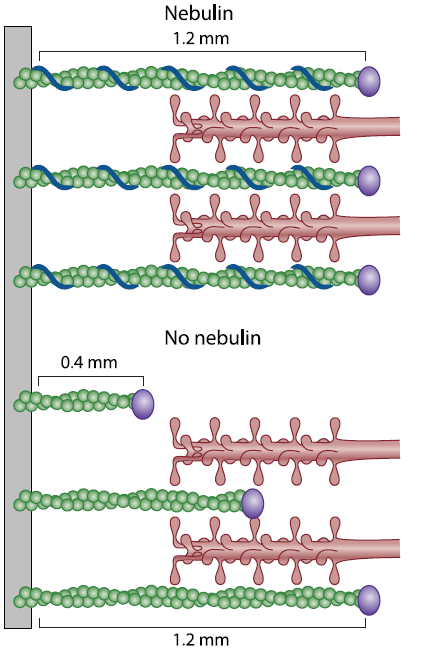
\includegraphics[scale=0.4]{Figures/Nebuline.png} 
\caption{Rôle de la nébuline dans le maintient de la longueur des filaments adéquate dans les cellules musculaires, d'après \cite{ottenheijm_lifting_2010}.\label{nebuline}}
\end{figure} 

Les nébulines sont des protéines stabilisantes dont le but est de fixer la longueur du filament d'actine auquel elles vont se lier, à la manière d'un étalon de mesure (\cite{ottenheijm_lifting_2010}, voir figure \ref{nebuline}). 



\subsection{Organisation en réseau de filaments}

Les filaments d'actine en évolution permanente sont liés entre eux mais également à la membrane plasmique et aux autres filaments du cytosquelette (microtubules et filaments intermédiaires). 


\subsubsection{Ancrage à la membrane}

Les cellules sont liées mécaniquement entre elles par des protéines transmembranaires, en particulier les cadhérines, qui relient leurs réseaux d'actine. Les caténines font la liaison entre les cadhérines et les filaments d'actine. 

L'ancrage du cytosquelette à la matrice extra-cellulaire se fait par l'intermédiaire d'une structure extraordinairement complexe, les adhésions focales. 
Au niveau des adhésions focales, des dizaines de protéines interagissent entre elles pour relier les intégrines enchâssées dans la membrane et les filaments d'actine. 
Je ne vais pas faire ici l'inventaire des protéines impliquées dans ces adhésions. 
À l'intérieur des adhésions focales, une signalisation complexe est à l'\oe uvre qui permet, en réponse à des forces extérieures, de construire une structure mécanosensible capable de déclencher des cascades de signalisation dans toute la cellule (\cite{geiger_environmental_2009}). 
En particulier, les petites GTPases Rac, Rho et Ras sont activées par des signaux provenant des adhésions focales soumises à des signaux mécaniques et régulent l'architecture du cytosquelette.
Je reviendrai plus loin sur la mécanique des adhésions focales.  

\subsubsection{Protéines de pontage}

Les filaments d'actine sont organisés en réseau par des protéines comme la filamine, la spectrine ou la transgeline. 

\begin{figure}
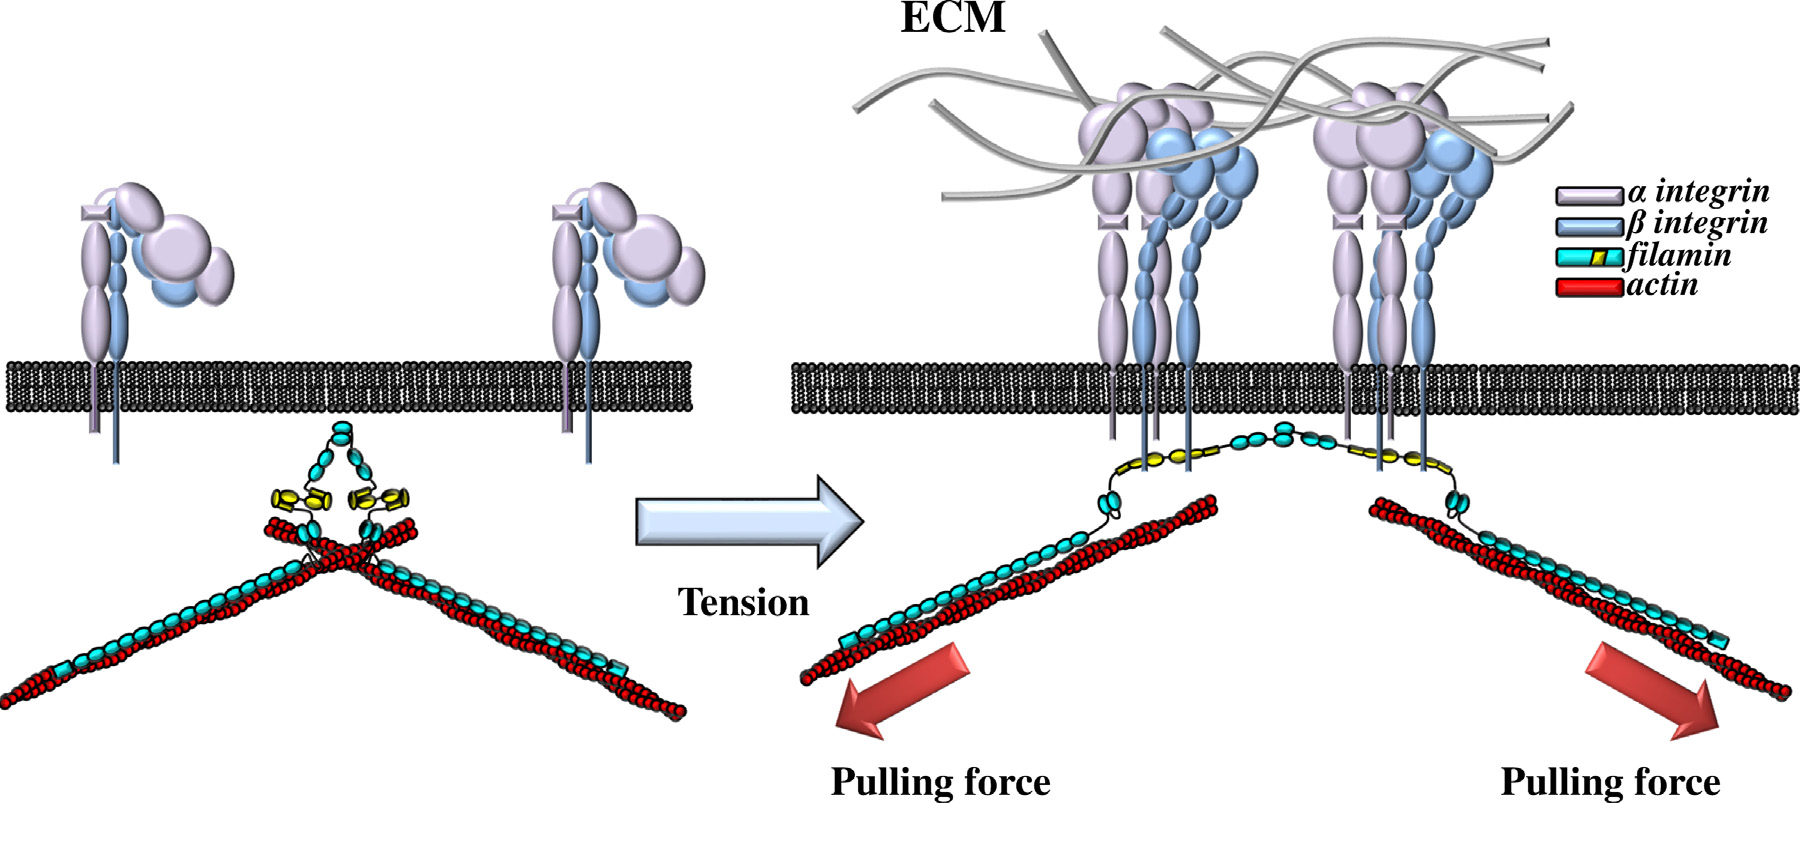
\includegraphics[scale=0.25]{Figures/filamine.png} 
\caption{Représentation d'un dimère de filamine se dépliant sous tension par (\cite{janostiak_mechanosensors_2014}) \label{filamine}}
\end{figure}

La filamine est un homodimère qui lie deux filaments d'actine. Elle peut se déformer sous la contrainte (\cite{furuike_mechanical_2001}), ce qui permet de doter le réseau d'actine à la fois d'une élasticité et d'une mécanosensibilité supplémentaire (\cite{kainulainen_cell_2002}).
La filamine peut également se lier à la membrane pour y ancrer le réseau d'actine (\cite{yamazaki_section:_2002}).


Lorsque son interaction avec les filaments est forte, l'$\alpha$-actinine peut lier des filaments en réseaux, alors que lorsque sa vitesse de dissociation est grande elle forme plutôt des faisceaux (\cite{wachsstock_affinity_1993}). Elle fait partie des protéines qui organisent les filaments d'actine dans les cellules musculaires, et sera donc évoquée à nouveau dans le chapitre 4. 


\subsubsection{Protéines de faisceau}

Ces protéines permettent de rassembler les filaments d'actine en faisceaux parallèles ou anti-parallèles. Cette architecture est retrouvée dans les filopodes, dans les fibres de stress ou dans les microvillosités.

Il peut y avoir deux domaines de liaison à l'actine sur la même protéine, comme c'est le cas pour la fimbrine, l'écart entre deux filaments est alors faible et le faisceau maintenu serré. 
Des protéines se liant à l'actine peuvent également former des dimères ou des multimères où chaque sous-unité lie un filament. L'$\alpha$-actinine permet ainsi de former des fibres de filaments anti-parallèles. La jonction entre les filaments est plus souple et moins serrée. 

\subsubsection{Lien avec les autres filaments du cytosquelette}

Le cytosquelette d'actine est relié aux réseaux de filaments intermédiaires et aux microtubules par des protéines capables de se lier à deux ou aux trois types de filaments. 
Par exemple, la plectine et les nesprines permettent de connecter les microtubules et les filaments d'actine au réseau de lamines de la membrane nucléaire, et donc de transmettre les contraintes jusqu'au noyau (\cite{wiche_role_1998},\cite{tapley_connecting_2013}). 
Les WHAMM en sont un autre exemple, elles se lient aux microtubules et à la membrane et nucléent des filaments d'actine. 



\subsubsection{Moteurs moléculaires : myosines}

Les myosines sont des moteurs moléculaires qui se déplacent sur l'actine en consommant de l'ATP. Il en existe chez tous les eucaryotes, mais leur homologie n'est pas aussi grande que celle de l'actine, car elles ont des fonctions différentes. Dans le génome humain, on dénombre une quarantaine de gènes pour la myosine, qui forment 17 groupes.

\begin{figure}
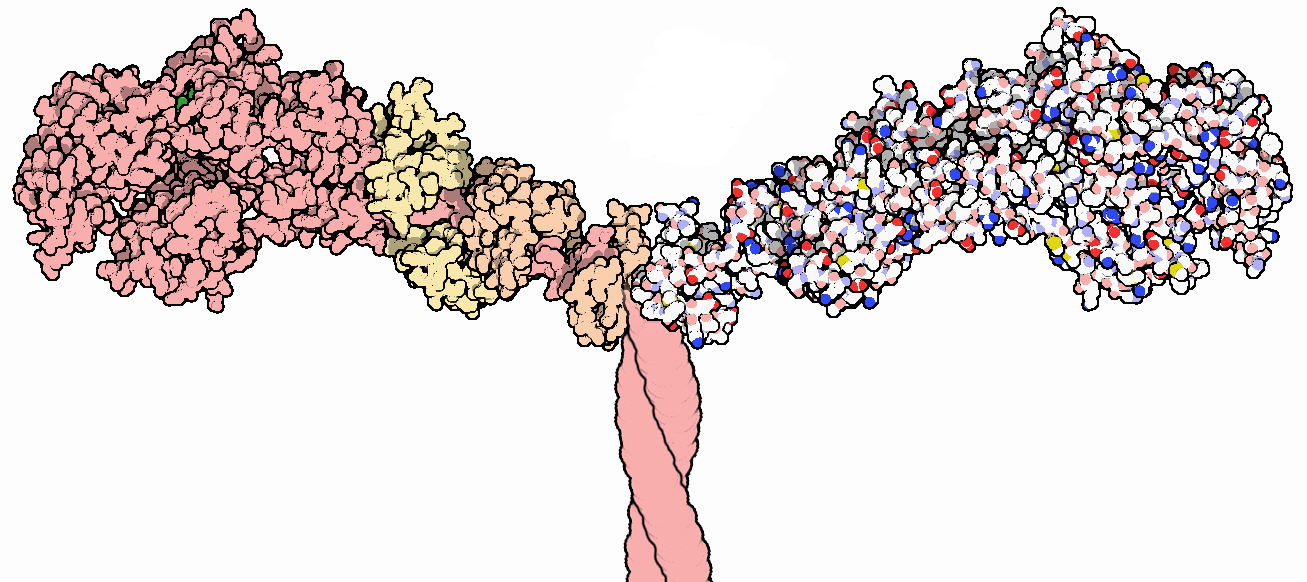
\includegraphics[scale=3]{Figures/18-Myosin-1b7t.png} 
\caption{Structure d'une myosine à deux têtes : en rouge la chaîne lourde, en jaune et orange les deux chaînes légères. Les queues des deux chaînes lourdes sont enroulées l'une autour de l'autre. Illustration tirée de l'article du mois de la Protein Data Bank sur la myosine (\cite{goodsell_molecule_2010}) \label{myosin}}
\end{figure}

La myosine II, aussi appelée \og conventionnelle \fg  est la plus étudiée. Elle est présente en quantité importante dans le muscle, car avec l'actine elle permet la contraction musculaire. 

Les myosines ont une tête qui peut se lier à l'actine en filament, un cou  qui sert de levier et de régulateur, et une queue qui sert souvent à former un dimère, et éventuellement à se lier à un cargo. On les appelle \og chaînes lourdes \fg par opposition aux \og chaînes légères \fg, qui ne sont pas à proprement parler des myosines mais qui sont des protéines qui vont se lier au cou des \og chaînes lourdes \fg pour les réguler. On peut en voir une représentation par la Protein Data Bank en figure \ref{myosin}.

Par exemple, pour la contraction musculaire, deux chaînes lourdes de myosine II s'associent en dimère par leur queue, et quatre chaînes légères s'ajoutent au niveau des deux cous. Les queues de milliers de myosines sont tressées en un filament épais, qui va coulisser par rapport au filament d'actine, appelé en comparaison filament fin, sous l'action du cycle de la myosine (voir figure \ref{myosin_cycle}). La structure et la contraction musculaires seront détaillées dans le chapitre 4. 

Le dimère a alors deux têtes pouvant se lier à l'actine, et va s'en servir pour avancer le long du filament, à la manière dont un alpiniste plante un piolet, se hisse puis détache le piolet pour le replanter plus loin, successivement pour les deux bras. Le cycle de la myosine est présenté en figure \ref{myosin_cycle}. 

\begin{figure}

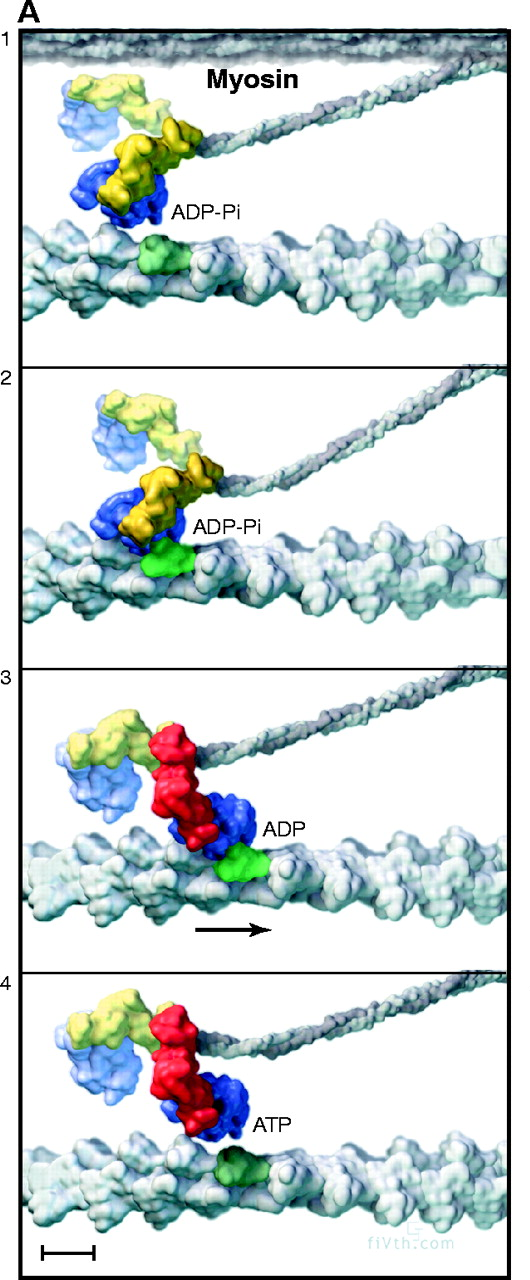
\includegraphics[scale=0.4]{Figures/Myosin.png} 
\caption{Reconstitution du cycle de la myosine à l'aide des données de la Protein Data Bank par (\cite{vale_way_2000}). Ici deux myosines forment un dimère doté de deux têtes et d'une longue queue qui lui permet de se lier au filament épais, composé de milliers de queues de myosines.  1 $\rightarrow$ 2 : La tête de myosine liée à un ADP + phosphate se lie au filament d'actine. 2 $\rightarrow$ 3 : Le phosphate est libéré, causant un changement de conformation du levier (en jaune sur l'image 2, en rouge sur l'image 3) qui fait coulisser un filament par rapport à l'autre. 3 $\rightarrow$ 4 : L'ADP est remplacé par un ATP, ce qui provoque le détachement du filament d'actine. 4 $\rightarrow$ 1 : L'ATP est hydrolysé en ADP+Pi, ce qui arme la tête de myosine, préparant le cycle suivant. La barre représente 6nm. \label{myosin_cycle}}
\end{figure} 



Certaines myosines ont un rôle analogue à celui des moteurs moléculaires associés aux microtubules et transportent des molécules le long des filaments, en général en direction de l'extrémité + , seule la myosine VI se déplace en sens inverse. Certaines autres, comme les myosines I n'ont qu'une seule tête. 


Les faiceaux anti-parallèles d'actine peuvent être liés par des paires de dimères de myosine, qui vont marcher en sens opposé sur les deux filaments, et donc les déplacer l'un par rapport à l'autre. Si les deux filaments sont liés par ailleurs dans le réseau, il va être mis sous tension par ces moteurs moléculaires. 




\section{Rôle mécanique de l'actine : du filament au cytosquelette}

Le cytosquelette est une structure multi-échelle, allant de l'échelle des protéines, à l'échelle de la cellule toute entière, en passant pas l'échelle des filaments et des réseaux de filaments. Il peut ressentir et exercer des forces à toutes les échelles. 


Dans cette partie, il ne s'agit pas de parler des propriétés mécaniques du cytosol ou de la cellule, mais d'expliquer comment les filaments peuvent générer des forces et comment ils réagissent à des forces. 

\subsection{Mécanique du filament d'actine}

Le filament d'actine en lui-même est à la fois générateur et senseur de forces. 

 \subsubsection{Longueur de persistance}
La longueur de persistance $\ell_p$ est un moyen de quantifier la corrélation entre l'orientation des différents segments d'un polymère soumis aux fluctuations thermiques. Si l'on considère un polymère de longueur $L$ auquel on attribue une abscisse curviligne $s$, avec $\vec{t_s}$ la tangente au polymère en $s$, alors on a la relation : 
$$ \langle \vec{t_0}\cdot \vec{t_s} \rangle_L \propto e^{-L/\ell_p}$$

Au bout de quelques longueurs de persistance, l'information de l'orientation du polymère en $s=0$ est perdue. 

La longueur de persistance dépend de l'énergie thermique disponible pour agiter le filament : elle diminue lorsque la température augmente. 

On peut également définir l'énergie de courbure d'un filament de longueur $L$, de rayon $a$ et de module élastique de courbure $\kappa$ : 
$$ E= \frac{\kappa}{2L} \int_0^L \left( \frac{\partial \theta}{\partial s} \right) ds \approx \frac{\kappa L}{2R^2}$$
 où $R$ le rayon de courbure du filament.  
 On définit alors la longueur de persistance comme la longueur pour laquelle l'énergie de courbure devient comparable à l'énergie thermique : 
 $$ E (L=l_p,R=l_p) = \frac{k_B T}{2} = \frac{\kappa l_p}{2 l_p^2}$$ 
 $$ l_p = \frac{\kappa}{k_B T}$$
 
 
Le filament d'actine subit un vieillissement par l'hydrolyse de l'ATP des monomères qui le composent. Le changement de conformation induit par l'hydrolyse de l'actine a des conséquences sur les propriétés mécaniques du filament. 
Un filament d'actine ATP a une longueur de persistance de 15 micromètres, contre 9 micromètres pour un filament d'actine ADP (\cite{isambert_flexibility_1995}). Le vieillissement du filament le rend donc plus déformable et plus souple. 
Les protéines attachées au filament peuvent également, en stabilisant une conformation, changer sa rigidité. Un filament stabilisé par la phalloïdine ou par la tropomyosine voit sa longueur de persistance augmentée à 18 et 20 microns respectivement (\cite{isambert_flexibility_1995}). Au contraire, la conformation stabilisée par la cofiline n'a qu'une longueur de persistance de 2,2 microns (\cite{mccullough_cofilin_2008}). 

Un même filament d'actine peut évidemment être le lieu de toutes ces modifications en même temps. Souvent l'extrêmité + des filaments est riche en actine ATP alors que l'extrémité $-$ est riche en actine ADP, ce qui crée un filament plus rigide d'un côté et plus flexible de l'autre. 

\subsubsection{Couplage traction-torsion}

L'hélice que forme le filament peut adopter des conformations différentes, en particulier en ce qui concerne l'angle de rotation entre les monomères successifs. 
Une force tirant sur le filament va alors favoriser une conformation à faible torsion, ce qui va rendre la fixation de la cofiline, qui stabilise le filament dans une conformation à grande rotation, beaucoup plus difficile. 
Il en résulte que la cofiline est moins efficace sur les filaments qui sont en tension (\cite{hayakawa_actin_2011}), induisant une préservation automatique des filaments sous contrainte par rapport aux filaments libres. 
Au contraire, la formine mDia1, qui est un élongateur des filaments, et la profiline sont plus efficaces sur les filaments soumis à une tension (\cite{higashida_f-_2013}). 
La conformation de l'actine est alors un senseur de contrainte qui va encourager la préservation et l'élongation des filaments qui ressentent une force de traction. 

Les filaments d'actine semi-flexibles peuvent également être courbés, en particulier au voisinage de la membrane. 
À cause de l'organisation hélicoïdale des monomères, la courbure d'un filament d'actine exerce également une torsion sur ce filament, ce qui rend leur modélisation encore plus complexe. 
Des observations \textit{in vitro} sur des filaments d'actine courbés et immobilisés montrent que le facteur de nucléation Arp2/3 se lie préférentiellement au côté convexe d'un filament d'actine courbé (\cite{risca_actin_2012}). 

\subsubsection{Les myosines}

Le cycle de la myosine (voir \ref{myosin_cycle}) est lui-même dépendant des forces qui peuvent être appliquées à la myosine. 
L'application d'une force de 1,6pN poussant la myosine vers sa conformation finale divise par deux la durée que la myosine va passer attachée au filament 
%en facilitant le changement de conformation 
(\cite{veigel_load-dependent_2003}). 
Inversement, l'application de la même force en sens opposé multiplie par deux la durée d'attachement. 
En fait, la durée que la myosine passe attachée au filament d'actine dépend exponentiellement de la force exercée, dans la gamme -2pN $-$ 2pN (\cite{veigel_load-dependent_2003}). 

Le régime de fonctionnement des myosines va donc être dépendant de la tension du réseau. 
%Les forces transmises par les filaments sous tension vont donc influer sur la cinétique du cycle de la myosine, et donc sur les forces qui vont être exercées par elle sur les filaments d'actine. 

\subsubsection{La croissance du filament comme source de force}

La croissance des filaments peut elle-même être une source de forces. Par exemple, un filament en croissance proche de la membrane plasmique s'appuie sur elle et sur le réseau d'actine derrière lui dans la cellule. 
Ces forces peuvent être utilisées pour pousser la membrane plasmique, créant une protrusion comme un filopode ou un lamellipode. Sous l'effet de l'agitation thermique, un monomère pousse la membrane. Si l'extrémité barbée d'un filament se trouve à proximité, le monomère peut alors rejoindre le filament. Ce qui était une fluctuation thermique devient alors une déformation pérenne de la membrane plasmique par le filament d'actine. 
La bactérie \textit{Listeria Monocytogenes} utilise également ce mécanisme pour se déplacer à l'intérieur des cellules qu'elle infecte : elle possède à sa surface la protéine ActA qui recrute Arp2/3 pour initier la polymérisation d'actine et VASP pour allonger les filaments. 


\begin{figure}[h!]
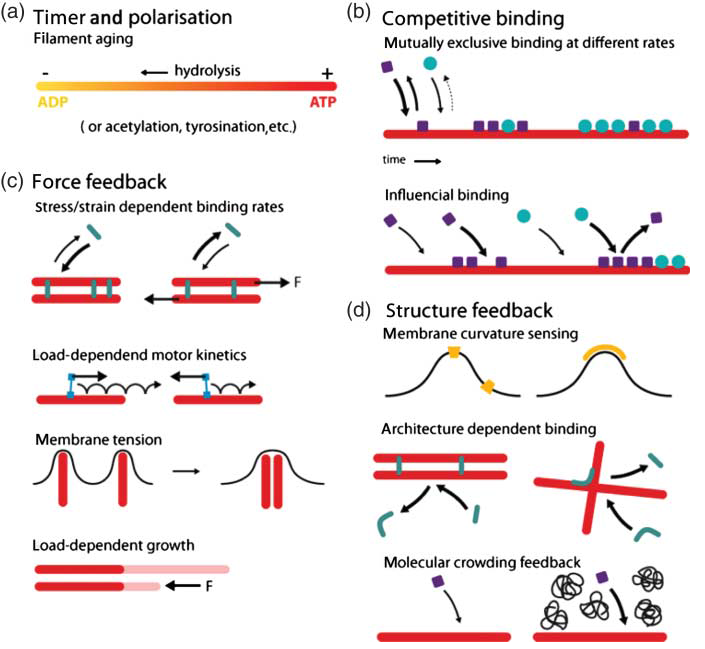
\includegraphics[scale=0.7]{Actine_phenomenon.png}
\caption{Présentation des différentes sources de sensibilité mécanique du cytosquelette d'actine au niveau du filament lui-même et des protéines interagissant avec lui, d'après la revue de (\cite{huber_emergent_2013})}
\end{figure}



\subsection{Mécanique des adhésions focales \label{adhesions}}

Les sites d'ancrage de la cellule dans la matrice extra-cellulaire sont la porte d'entrée des signaux mécaniques dans la cellule. Parmi les molécules qui constituent les adhésions focales, certaines réagissent directement lorsqu'elles sont soumises à des stimulations mécaniques. 

Lorsque la transmission des forces est coupée dans la cellule (par l'ajout de drogues qui inhibent la contractilité du cytosquelette), les adhésions focales disparaissent : la tension est nécessaire non seulement à leur constitution, mais également à leur maintien. Ces contraintes peuvent provenir de forces extérieures mais aussi de la contraction du cytosquelette sous l'action des moteurs moléculaires. 

\begin{figure}
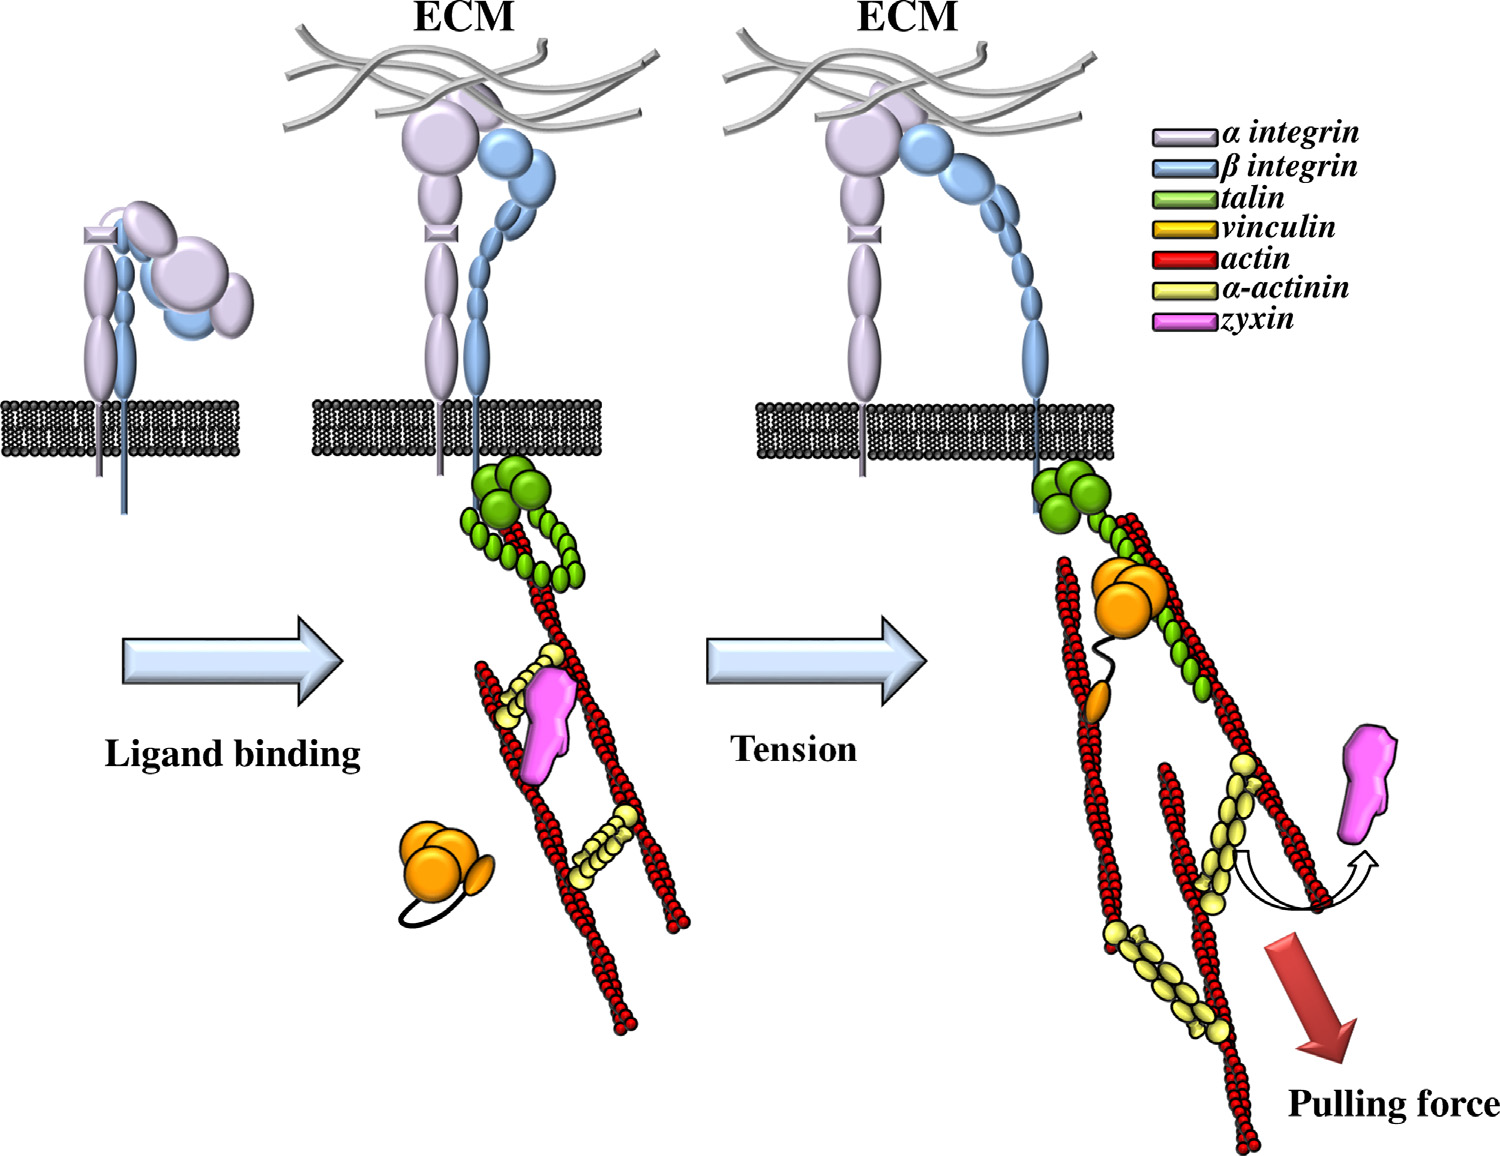
\includegraphics[scale=0.2]{Focal_adhesions_taline.png}
\caption{Dépliement de la taline sous tension, qui fait apparaître les sites cryptiques de liaison à la vinculine, d'après (\cite{janostiak_mechanosensors_2014})}
\end{figure}

En présence d'une force, les intégrines forment des agrégats et leur affinité pour le ligand augmente grâce à un changement de conformation. 
La taline relie les intégrines aux filaments d'actine. Dans la conformation initiale, elle est repliée sur elle-même. Lorsqu'elle est mise sous tension entre les intégrines et l'actine, elle se déplie, laissant apparaître des domaines de liaisons à la vinculine qui n'étaient pas précédemment accessibles (\cite{del_rio_stretching_2009}). 
L'arrivée des vinculines dans les adhésions focales dépend de la tension au niveau de l'adhésion (\cite{pasapera_myosin_2010}) et permet leur renforcement (\cite{galbraith_relationship_2002}). 

De façon similaire, la filamine, qui lie entre eux des filaments d'actine, peut être dépliée lors de tensions sur les filaments  (\cite{furuike_mechanical_2001}). Son domaine de liaison aux intégrines devient alors accessible, et la filamine ancre alors le cytosquelette à la matrice extra-cellulaire par l'intermédiaire des intégrines (\cite{yamazaki_section:_2002}). De plus, cela cause un changement de conformation des intégrines qui favorise la formation d'agrégats, renforçant l'adhésion. Cela est illustré par la figure \ref{filamine}.

Ce ne sont là que quelques exemples de protéines impliquées dans les adhésions focales, il en existe des centaines. Leur exemple montre qu'au premier niveau de contact avec l'environnement mécanique extérieur, les forces sont relayées en un signal biologique au niveau de la molécule individuelle, en changeant la conformation des protéines. 

\subsection{Mécanique du cytosquelette d'actine}

Les protéines organisant les filaments d'actine vont construire des structures à l'échelle de la cellule spécialisées dans l'exploration, le mouvement, le maintien ou le changement de forme \dots

Ces structures vont exercer des forces sur l'extérieur pour se tracter ou se propulser à l'aide de blebs ou de lamellipodes, maintenir la forme cellulaire en mettant sous tension le cortex sous la membrane plasmique et/ou en s'ancrant au substrat par les adhésions focales, ou au contraire changer complètement de forme lors de la phagocytose. 

Les cellules musculaires, qui exercent des forces pendant la contraction des muscles, ont une organisation très spécifique du cytosquelette d'actine  qui sera décrite au chapitre 4. 
%
%Le cytosquelette  a principalement été étudié par la motilité sur des surfaces planes et rigides de cellules comme les fibroblastes et les kératocytes. 
%Cependant, d'autres types cellulaires peuvent s'engager dans des mouvements ou des organisations du cytosquelettes très différentes. 
%C'est le cas par exemple des cellules du système immunitaire : par exemple les lymphocytes T patrouillant dans le système sanguin sont dotés d'un uropode qui leur permet de s'orienter à contre-courant (\cite{valignat_lymphocytes_2014}). Autre exemple, la phagocytose requiert une réorganisation polarisée rapide du cytosquelette à l'échelle de la cellules.
%C'est également le cas des cellules musculaires différenciées en myofibres, qui ont une organisation du cytosquelette extrêmement spécialisée pour la contraction musculaire, et qui seront décrites plus loin au chapitre 4. 
%
%Si les organisations décrites ici ont été particulièrement étudiées dans le cadre des fibroblastes et des kératocytes, elles font partie des mécanismes de migration de la plupart des cellules. 

\subsubsection{Le cortex}

\begin{figure}
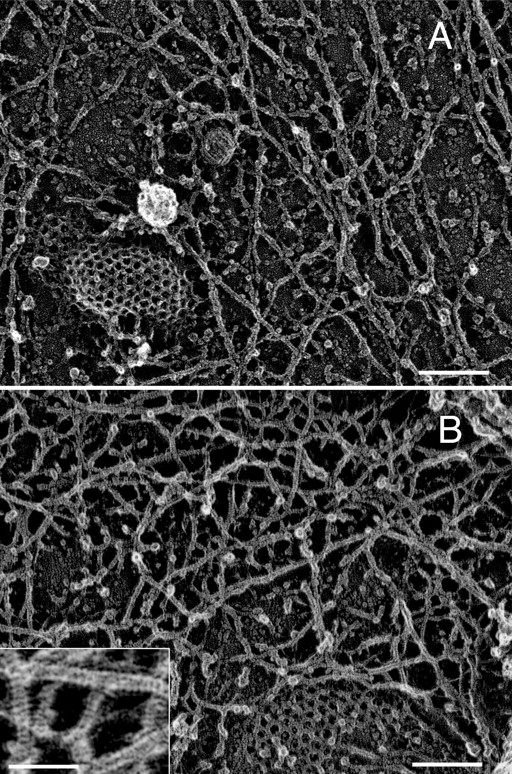
\includegraphics[scale=0.25]{Figures/cortex.png} 
\caption{Image en microscopie électronique du cortex d'actine sous la membrane, par \cite{morone_three-dimensional_2006}. La barre d'échelle de l'image du haut représente 100nm, celle du bas 50 nm. On peut également voir une cavéole.}
\end{figure}

La membrane plasmique est soutenue par un réseau d'actine de quelques centaines de nanomètres d'épaisseur appelé le cortex.

Le cortex est constitué d'un mélange entre un réseau ramifié par Arp2/3 et des faisceaux de filaments alignés. 
Il est attaché à la membrane plasmique par des protéines comme celles de la famille ERM (ezrine, radixine, moesine) (\cite{biro_cell_2013}). 

Il contient également des myosines qui mettent le réseau sous tension. Cette tension crée une pression vers l'intérieur de la cellule contrée par une différence de pression osmotique. L'équilibre entre les deux forces explique la forme ronde des cellules lorsqu'elles entrent en mitose (\cite{stewart_hydrostatic_2011}).
Lorsque le cortex d'actine est brisé ou détaché de la membrane localement, cette pression interne de la cellule provoque la formation d'une protrusion de la cellule appelée bleb (\cite{paluch_cortical_2005}).

Les blebs sont un moyen qu'a la cellule d'explorer l'espace. La protrusion de membrane est alors complétée par un réseau d'actine et des adhésions à partir desquels la cellule va pouvoir progresser vers l'avant \parencite{charras_blebs_2008}. 
Ce mode de déplacement a été particulièrement étudié chez les amibes comme Dictyostelium, c'est pourquoi il est dit \og amiboïde \fg.  

Ils peuvent également être le moyen d'équilibrer les forces dans une cellule en division, pour positionner correctement le fuseau mitotique (\cite{sedzinski_polar_2011}).

Le cortex et la membrane sont intimement couplés mécaniquement, au point qu'il est souvent difficile de séparer l'influence mécanique de la tension de la membrane de celle du cortex (\cite{campillo_mechanics_2012}). 
En aspirant le cortex dans une micropipette il est possible de tester sa résistance mécanique et de constater qu'elle dépend de l'activité des myosines (\cite{bergert_cell_2012}).  



\subsubsection{Le lamellipode}

\begin{figure}[h!]
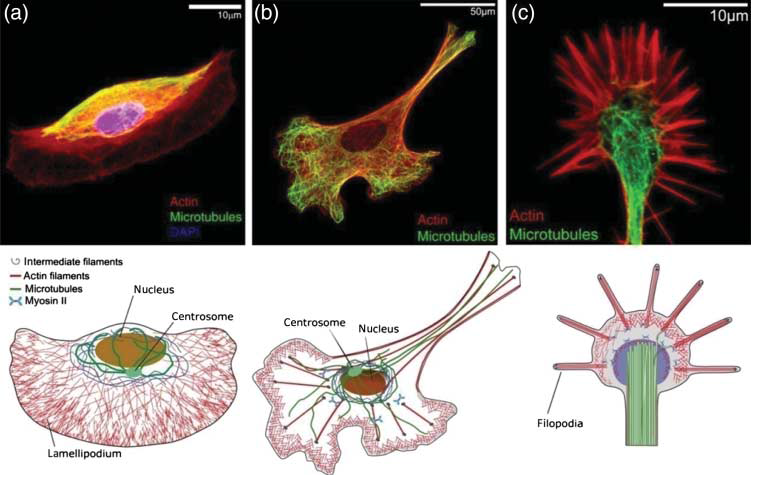
\includegraphics[scale=0.6]{Figures/lamellipode.png}
\caption{Images en microscopie de fluorescence et schéma représentatif d'un lamellipode de kératocyte, d'un lamellipode de fibroblaste et des filopodes d'un neurone, d'après \cite{huber_emergent_2013}. } 
\end{figure}

Le lamellipode est une structure plane à l'avant d'une cellule en mouvement, prenant la plupart du temps une forme en croissant. 

Sous la membrane, la GTPase Rac active Arp2/3 par l'intermédiaire du complexe WAVE, formant un réseau ramifié (\cite{lebensohn_activation_2009}). 
La croissance des filaments pousse alors le bord de la cellule vers l'avant, en s'appuyant sur les adhésions focales à l'arrière du lamellipode. 
La croissance du réseau ramifié créé par Arp2/3 est maintenu sous contrôle par les protéines de coiffage qui bloquent l'élongation excessive des filaments. 

Le flux rétrograde de l'actine entraîne les filaments vers l'arrière de la cellule où ils sont fragmentés et dépolymérisés. 
Certains sont assemblés en faisceaux contractiles par les myosines. 

À l'arrière de la cellule, le réseau d'actine est détruit sous l'action conjuguée de la tension de membrane (\cite{raucher_cell_2000}) et des myosines (\cite{wilson_myosin_2010}) et les adhésions disparaissent afin de permettre à la cellule d'avancer.

Le lamellipode est principalement lié aux déplacements sur une surface plane, comme en culture cellulaire ou à la surface d'un épithélium. 



\subsubsection{Les filopodes}

Les filopodes sont des protrusions consituées d'un faisceau d'actine dont les extrémité $+$ sont pointées vers l'extérieur. 
La croissance du filopode est principalement liée à celle des filaments du faisceau grâce à l'action des formines ou de Ena/VASP. 

Un filopode peut se former à partir de la convergence de filaments provenant d'un réseau branché au bord de la cellule (\cite{small_actin_1995}). Cependant, Arp2/3 n'est pas indispensable à la formation des filopodes (\cite{wu_arp2/3_2012}). 
Des protéines comme la fascine associent alors ces filaments en faisceau rigide, dont la croissance déforme la membrane plasmique. 

Les filopodes servent à explorer l'espace, initiant le contact avec la matrice extra-cellulaire ou avec d'autres cellules voisines. 
Certaines bactéries exploitent ce comportement pour être capturées et internalisées par la cellule (\cite{romero_atp-mediated_2011}). 
Après contact avec la bactérie, le filopode se rétracte rapidement, ramenant la bactérie vers sa cible.
La force exercée par un filopode en rétraction peut atteindre 10pN, à des vitesses de l'ordre de 100nm/s (\cite{vonna_micromechanics_2007},\cite{romero_atp-mediated_2011}). 



\subsubsection{Fibres de stress}

\begin{figure}
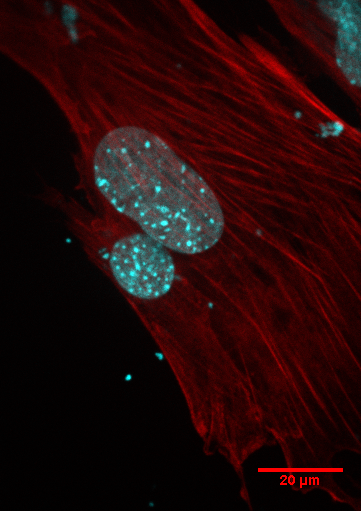
\includegraphics[scale=0.4]{Figures/Fibres_de_stress_dessous.png} 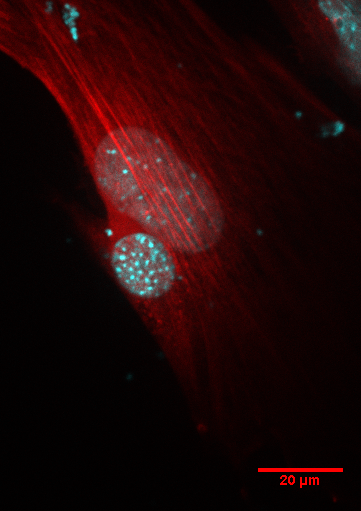
\includegraphics[scale=0.4]{Figures/Fibres_de_stress_dessus.png} 
\caption{Fibres de stress marquées avec de la phalloïdine (en rouge) sur deux myoblastes C2C12 étalés sur du PDMS. En cyan, l'ADN du noyau. L'image de gauche montre les fibres sur la face ventrale de la cellule, l'image de droite les fibres sur la face dorsale, au-dessus du noyau. }
\end{figure}
Les fibres contractiles sont constituées de faisceaux de filaments anti-parallèles liés par l'$\alpha$-actinine, associés à des myosines, trois éléments que l'on retrouve pour organiser les myofibres responsables de la contraction musculaire. \cite{lazarides_-actinin:_1975} observe des marquages de l'$\alpha$-actinine dans des myofibres et dans des cellules non musculaires et souligne une organisation périodique de l'$\alpha$-actinine qui est similaire dans les fibres de stress et dans les sarcomères.

Ces fibres sont mises sous tension par les myosines qui font coulisser les filaments les uns par rapport aux autres. 
Les adhésions focales et les jonctions adherens sont souvent connectées à des fibres de stress qui vont les maintenir sous tension. Comme déjà mentionné dans la section \ref{adhesions}, cette tension va activer des cascades de signalisation qui va renforcer ces adhésions. 

La création de fibres de stress et leur fonction de renforcement des adhésions est régulée par la petite GTPase RhoA, dont je reparlerai plus en détail dans le chapitre suivant. RhoA active des formines qui favorisent l'élongation des filaments, désactive la cofiline, ce qui contribue à préserver les longs filaments de la polymérisation, et augmente l'activité des myosines qui mettent les fibres sous tension. 

Les fibres de stress sont des structures qui apparaissent essentiellement dans les cellules étalées sur un substrat plan, beaucoup plus rarement dans une matrice à trois dimensions. 



\section{Rôle régulateur de l'actine nucléaire}

L'actine nucléaire est plus difficile à observer que l'actine cytoplasmique, c'est pourquoi son existence et son rôle ont été ignorés pendant longtemps. 
Aujourd'hui, l'amélioration des techniques de microscopie et le développement de techniques spécifiques (comme des sondes dotées d'un NLS) permettent de confirmer l'existence d'actine nucléaire tant en monomères qu'en filaments (\cite{mcdonald_nucleoplasmic_2006},\cite{baarlink_nuclear_2013}). 
De plus, un grand nombre de protéines liées à l'actine, comme la profiline, la cofiline, Arp2/3, N-WASP, les formines, MICAL et des myosines, sont également présentes dans le noyau, créant toutes les conditions pour qu'un véritable nucléosquelette soit constitué dans la cellule. 
La profiline et la cofiline aident respectivement à l'export et à l'import des monomères d'actine par les pores nucléaires, jouant ainsi un double rôle de régulation de l'actine nucléaire. 


\subsection{L'actine G nucléaire dans les complexes}

80\% de l'actine nucléaire est sous forme de monomères \parencite{mcdonald_nucleoplasmic_2006}. Ces monomères vont s'incorporer dans un grand nombre de complexes indispensables à la transcription de l'ADN en ARN et à la maturation de l'ARN. 

Chez les eucaryotes, la transcription de l'ADN en ARN est effectuée par trois ARN Polymérases. Il a été montré que l'actine est nécessaire à l'activité des trois ARN Polymérases ( \cite{ye_nuclear_2008}, \cite{hofmann_actin_2004} \cite{hu_role_2004}).

L'actine est également liée aux ribonucléoprotéines hétérogènes (hnRNP) présentes sur les pré-ARN messagers pendant et après leur transcription \parencite{kukalev_actin_2005}. Les hnRNP empêchent ces ARN messagers qui doivent encore subir des étapes de maturation de se replier sur eux-mêmes (ce qui pourrait interférer avec leur traitement) ou d'être exportés avant d'avoir été traités. Elles peuvent également se lier à la machinerie d'épissage. 

Les complexes de remodelage de la chromatine font passer la chromatine d'un état très compact impossible à transcrire à un état où l'expression des gènes devient possible. L'actine fait partie de plusieurs types de complexes de remodelage de la chromatine comme SWI/SNF, RSC et BAF (revue par \cite{farrants_chromatin_2008}). 

Enfin, l'actine monomérique bloque également l'activité de la DNase I dans le noyau et l'empêche de couper l'ADN en petits morceaux (\cite{lazarides_actin_1974}). 

\subsection{Les filaments d'actine et la myosine nucléaires}

20\% de l'actine nucléaire est présente sous la forme de filaments \parencite{mcdonald_nucleoplasmic_2006}. Les nucléateurs comme Arp2/3 (\cite{yoo_novel_2006}) et les formines (\cite{baarlink_nuclear_2013}) sont présents dans le noyau, aux côtés d'élongateurs spécifiques comme l'émerine (\cite{ho_lamin_2013}). 
Des myosines, comme la Nuclear Myosin 1 (NM1) (\cite{nowak_evidence_1997})  et la myosine VI sont présentes dans le noyau et ont un rôle essentiel dans la transcription. 

L'actine, mais également N-WASP et Arp2/3 sont nécessaires à la transcription efficace par l'ARN Polymérase II (\cite{yoo_novel_2006}). Les drogues empêchant la formation de filaments comme la latrunculine ou la cytochalasine D perturbent la transcription par PolII (\cite{mcdonald_nucleoplasmic_2006}).

La NM1 et l'actine se lient à PolI pour la transcription des gènes ribosomaux. La NM1 remodèle localement la chromatine dans une conformation favorable à la transcription (\cite{nowak_evidence_1997}).

Enfin, l'émerine, qui relie des filaments d'actine aux lamines qui enveloppent le noyau, joue un rôle essentiel dans l'organisation de l'hétérochromatine (revue par \cite{gieni_actin_2009}). 


Le noyau contient tous les éléments nécessaires à la formation d'un nucléosquelette mécaniquement fonctionnel : nucléateurs, élongateurs, protéines de pontage et moteurs moléculaires. 
Ce nucléosquelette est relié au cytosquelette par différentes protéines de la membrane nucléaire qui lient l'actine F, les filaments intermédiaires, les microtubules et les centrosomes. 
Dans le cas de l'actine, les nesprines et Sun 1 et 2 font la liaison entre les filaments d'actine du cytoplasme et les lamines, qui font la liaison avec les filaments nucléaires et la chromatine grâce à l'émerine. 





%\end{document}



\documentclass{report}
\usepackage[T1]{fontenc}
\usepackage[utf8]{inputenc}
\usepackage[francais]{babel}
\usepackage{amsmath}
\usepackage{graphicx}
\usepackage[backend=biber,style=authoryear]{biblatex}
\usepackage[colorlinks,linkcolor=blue]{hyperref}

\addbibresource{biblio.bib}

\begin{document}
\chapter*{MRTF-A}
En 2001, \cite{mercher_involvement_2001} 
décrivent une translocation impliquée dans les leucémies aigües mégacaryocytiques. 
Il s'agit de la translocation d'un gène du chromosome 1 sur le chromosome 22, le gène fusion est nommmé One-Twenty-Two-Megakaryocytic-Acute-Leukemia (OTT-MAL). 
Les fonctions des deux gènes qui ont fusionné est alors inconnue. 

En 2002, deux homologues de la myocardine sont identifiés dans le génome humain par \cite{wang_potentiation_2002} et sont nommés Myocardin-Related Transcription Factor A et B (MRTF-A/B).
MRTF-A correspond au gène du chromosome 22 MAL (ou MKL1) et MRTF-B à un gène du chromosome 16 (MAL16 ou MKL2). 
Un homologue est également découvert chez la souris et nommé Basic, SAP et Coil-coil (BSAC) \parencite{sasazuki_identification_2002}. 

Alors que cette protéine sera appelée dans la suite de ce document MRTF-A, elle pourra être identifiée indifféremment comme MAL, MKL1 ou BSAC dans la bibliographie. 

\section{MRTF-A, cofacteur de Serum Response Factor}

La fonction principale des protéines de la famille des myocardines est l'activation du facteur de transcription Serum Response Factor. 

\subsection{Serum Response Factor}

Serum Response Factor est un facteur de transcription qui fait partie de la famille MADS (MCM-1, Agamous, Deficiens, SRF). SRF est présent en un seul exemplaire dans le génome humain mais peut être transcrit en 4 isoformes. 
La protéine SRF comprend un signal de localisation nucléaire (NLS), une boîte MADS composée du site de liaison à l'ADN et d'un domaine de dimérisation, et d'un domain de transactivation auquel se fixent ses cofacteurs. 

Un dimère SRF se fixe sur une séquence consensus de nucléotides sur l'ADN appelée boîte CArG : CC(A/T)$_{6}$GG, ou sur une séquence CArG-like, qui diffère du consensus d'une seule base, avec une affinité plus faible. Le gène srf contenant lui-même deux boîtes CArG, il est sa propre cible, dans une boucle de rétro-action positive. 

\subsection{Les cofacteurs de SRF : TCF et MRTF}

Serum Response Factor n'est lui-même qu'un transactivateur faible, mais il peut être activé par deux grandes familles de cofacteurs : les Ternary Complex Factors, et les Myocardin-Related Transcription Factor. 

Les deux familles ne sont pas concurrentes pour se lier à SRF : la plupart des sites sur l'ADN sont spécifiques de l'une ou l'autre des familles de cofacteurs (\cite{esnault_rho-actin_2014}). Même lorsque les MRTF sont séquestrées dans le cytoplasmes, les TCF ne les remplacent pas sur les sites de liaison à SRF. 

Un ChIP-seq sur des fibroblastes 3T3 a estimé que 921 gènes sont susceptibles d'être régulés par MRTF/SRF en réponse au sérum, et 76 gènes par TCF/SRF (\cite{esnault_rho-actin_2014}), ce qui représente entre 3 et 4\% du génome. Les MRTF sont donc un élément important de la régulation transcriptionnelle, et l'acteur principal de la régulation de SRF. 

\emph{Les autres cofacteurs de SRF ? }


\subsubsection{Ternary Complex Factors}

Elk1, Net et SAP-1 sont trois coactivateurs de SRF de la même famille, les TCF. Ils possèdent un domaine qui leur permet de se lier à des sites spécifiques sur l'ADN (Ets Binding Sites). 
Lorsqu'un site Ets et une boîte CArG sont adjacents, ils forment un Serum Response Element (SRE). La formation d'un complexe TCF-SRF sur un SRE déclenche la transcription du gène cible. 

Les TCF sont phosphorylées et activées par les MAPK (Mitogen Activated Protein Kinases). 


\subsection{La famille Myocardine}

Cette famille de cofacteurs de SRF comprend la myocardine, MRTF-A et MRTF-B. 

La myocardine se présente sous deux isoformes, une forme cardiaque et une forme spécifique au muscle lisse. Les deux sont exclusivement localisées dans le noyau et sont constitutivement actives, en raison de motifs RPEL déficients ou incomplets. 

Les Myocardin-Related Transcription Factors A et B sont exprimées dans un grand nombre de tissus : muscles cardiaques, lisses et squelettiques, neurones, cellules épithéliales, mégacaryocytes \dots Contrairement à la myocardine, les MRTF peuvent être séquestrées dans le cytoplasme, ce qui les empêche d'activer SRF et la transcription. La régulation de la localisation de MRTF est assurée par l'actine, qui peut former un complexe avec la partie N-terminale des MRTF. 




\section{Rôles de MRTF-A}
Depuis sa découverte au début des années 2000, de nombreux rôles de MRTF-A ont été mis en évidence dans des types cellulaires et dans des tissus très divers. 
\subsection{Embryogenèse}

Les MRTF sont exprimées dès le jour 10 du développement de l'embryon (\cite{wang_potentiation_2002}), dans tous les tissus. La délétion de MRTF-B entraîne l'échec de la gastrulation, et donc une fin précoce de l'embryogenèse (\cite{kalita_mkls:_2012}). Au contraire, 60\% des mutants MRTF-A$^{-/-}$ sont viables et atteignent l'âge adulte, les autres étant perdus pendant l'embryogenèse car souffrant de défauts cardiaques. Les mutants survivants sont dépourvus de ces anomalies cardiaques, et vivent jusqu'à l'âge adulte (\cite{li_requirement_2006},\cite{sun_acute_2006}). Cependant, les femelles souffrent d'un défaut de formation de la glande mammaire,  lié à une apoptose précoce des cellules myoépithéliales qui déclenchent l'éjection du lait. Il apparaît donc que chez la souris, tandis que MRTF-B est indispensable à l'embryogenèse, l'absence de MRTF-A peut être compensée dans la plus grande partie des tissus. 
Les souris possédant un gène mutant dominant négatif de MRTF-A sont en revanche de plus petite taille, ne bougent pas et ne survivent que quelques jours, principalement à cause des défauts de musculature de leur diaphragme (\cite{li_requirement_2005}). 

\subsection{Régulation de la masse musculaire}



\subsection{Transition EMT}
\subsection{MRTF-A et cancers}

\newpage
\section*{Structure de MRTF-A}

\begin{figure}
\center
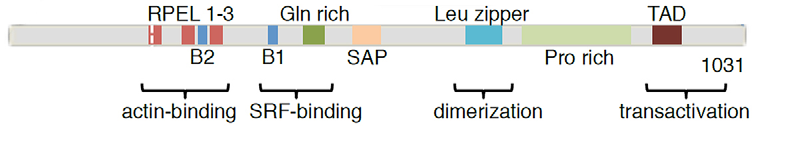
\includegraphics[scale=0.5]{MRTFA_structure.png}
\caption{Structure de MRTF-A \parencite{scharenberg_tgf-_2014}}
\end{figure}
 \subsection{Les motifs RPEL}
 
 La partie N-terminale de MRTF-A contient trois motifs RPEL consécutifs, qui peuvent se lier aux monomères d'actine (\cite{posern_mutant_2004}, \cite{mouilleron_molecular_2008}) avec des affinités variables, les deux premiers motifs se liant plus fortement que le troisième (\cite{guettler_rpel_2008}). La structure détaillée du complexe montre que les trois motifs RPEL se lient à 3 à 5 monomères d'actine selon la concentration en monomères d'actine. (\cite{hirano_sensing_2011}, \cite{treisman_structure_2011}). 
 
 Deux domaines basiques, B2 et B3 sont inclus dans les motifs RPEL et forment un signal de localisation nucléaire (NLS) bipartite (\cite{rajakyla_actin-regulated_2010}). Lorsqu'il n'y a pas d'actine sur les motifs RPEL, ce NLS peut se lier au complexe Importine$\alpha / \beta$ (\cite{hirano_sensing_2011},\cite{rajakyla_actin-regulated_2010}) et MRTF-A est importée dans le noyau de la cellule, où se trouve SRF. En présence de suffisamment de monomères, le NLS est recouvert par l'actine liée aux RPEL, MRTF-A reste cytoplasmique (Posern 2002, \cite{miralles_actin_2003},\cite{posern_mutant_2004}). 
 
 MRTF-A est exportée du noyau par Crm1 (\cite{vartiainen_nuclear_2007},\cite{hayashi_differences_2013}). \emph{Ces deux articles se contredisent sur la question de la liaison à l'actine : le premier prétend qu'elle est indispensable, le second qu'elle empêche l'export} 
 
 Les motifs RPEL sont donc la clé de la régulation de MRTF-A par l'actine : selon la concentration en monomères d'actine, MRTF-A est localisée dans le cytoplasme en cas d'excès et dans le noyau, où se trouve SRF, en cas de manque. Lorsque le domaine RPEL est muté ou absent, la protéine est constitutivement nucléaire (\cite{miralles_actin_2003}), comme la myocardine, dont les motifs RPEL ne sont plus fonctionnels (\cite{guettler_rpel_2008}). 
 
 \subsection{La région basique et SRF}
 La région B1 est le site de liaison de MRTF-A à SRF. MRTF-A s'attache préférentiellement à SRF en dimère (\cite{miralles_actin_2003}). Le complexe MRTF-A-5actines ne peut pas se lier à SRF et l'activer, la présence de MRTF-A dans le noyau n'est donc pas suffisante pour activer SRF, il faut également que la concentration en G-actine dissocie le complexe (\cite{vartiainen_nuclear_2007}). 
 \subsection{Leucine zipper et oligomérisation}
 MRTF-A/B peuvent former des homo ou des hétérodimères (\cite{miralles_actin_2003}). Un dominant négatif pourra ainsi bloquer une protéine WT dans un hétérodimère non fonctionnel (\cite{selvaraj_megakaryoblastic_2003},\cite{cen_myocardin/mkl_2004}, \cite{li_requirement_2005},\cite{rajakyla_actin-regulated_2010}). La formation des dimères n'est pas indispensable à la fonctionnalité de MRTF-A, les mutations dans cette région réduisent son efficacité sans l'inhiber totalement (\cite{selvaraj_megakaryoblastic_2003}). 
 OTT-MAL est également capable de former des hétérodimères avec les MRTF, et donc de perturber leur équilibre. 
 
 \subsection{SAP et TAD}
 
Dans les cellules épithéliales, il a été montré qu'un groupe de gènes est activé par MRTF-A et nécessite particulièrement la zone SAP, tout en étant indépendant de SRF (\cite{asparuhova_transcriptional_2011}, \cite{gurbuz_sap_2014}) 
 
 \subsection{Phosphorylation}
	MRTF-A peut être phosphorylée (\cite{miralles_actin_2003},\cite{cen_myocardin/mkl_2004},).Dans les neurones, la phosphorylation de MRTF-A par ERK1/2 est même la voie principale de régulation de son activité, car la protéine est toujours nucléaire, mais elle n'active SRF qu'une fois phosphorylée (\cite{kalita_role_2006}).
	
 \subsection{Isoformes}
 D'après \cite{scharenberg_tgf-_2014}, il existe 2 isoformes de MRTF-A chez l'humain, une version longue (MRTF-A\_L) et une courte(MRTF-A\_S). La version longue présente 80 acides aminés avant le premier motif RPEL, contre 15 seulement pour la version courte. Cette dernière contient deux TAD de 9 acides aminés (9aaTAD), un à l'extrémité C-terminale, et un à l'extrémité N-terminale spécifique à cet isoforme. Une surexpression de MRTF-A\_S est observée en réponse à TGF-$\beta$ ou à une contrainte cyclique dans les cellules épithéliales. 
 
 

\section{En amont de MRTF-A : voie de signalisation et régulation de l'actine} 
\subsection{Régulation de l'actine}
\subsection{Les protéines liées à l'actine}
\subsection{La voie RhoA}
\subsection{MICAL2}

\section{En aval de MRTF-A : SRF et gènes cibles}

\printbibliography
\end{document}

%\documentclass{report}
%\usepackage[T1]{fontenc}
%\usepackage[utf8]{inputenc}
%\usepackage[francais]{babel}
%\usepackage{amsmath}
%\usepackage{graphicx}
%\usepackage[backend=biber,style=authoryear,bibencoding=utf8]{biblatex}
%\usepackage[colorlinks,linkcolor=blue]{hyperref}
%\newcommand{\micro}{$\mathrm{\mu}$}
%\addbibresource{biblio2.bib}
%
%
%\begin{document}
\chapter{De la cellule au muscle}


\begin{center}
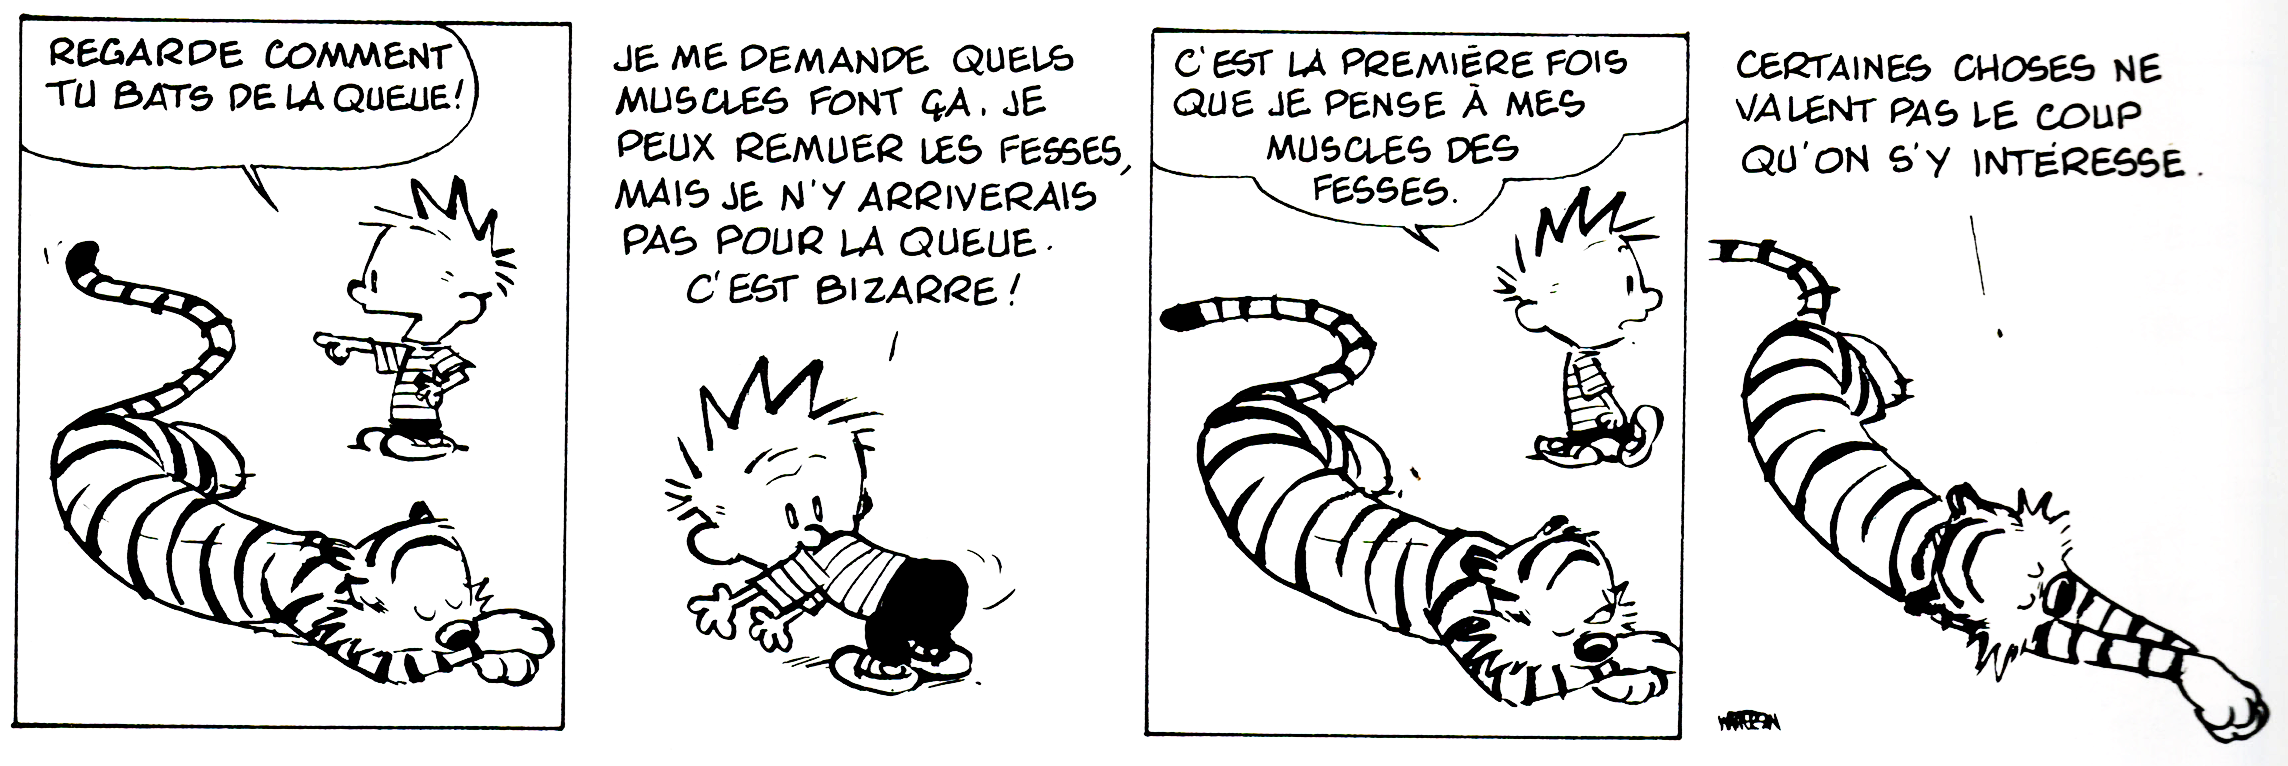
\includegraphics[scale=0.7]{Chapitre4.png}
\end{center}
\newpage

Les muscles représentent environ 40\% de la masse totale d'un humain adulte. Ils participent à tous les phénomènes indispensables à notre vie : ils nous permettent de nous mouvoir, d'exercer des forces sur notre environnement, mais aussi de respirer, de faire circuler le sang, de digérer \dots 
Il existe trois principaux types de muscles : lisses, cardiaque, et squelettiques. Les muscle lisses, comme ceux que l'on trouve le long du tube digestif ou des vaisseaux sanguins, mais aussi dans la vessie ou l'utérus, ne peuvent pas être contrôlés volontairement. 
Le muscle cardiaque, présent uniquement au niveau du c\oe ur, a une organisation spécifique qui lui permet de maintenir des contractions régulières et permanentes, assez puissantes pour faire circuler le sang dans le système circulatoire. 
Les muscles squelettiques sont les seuls que nous contrôlons volontairement. Comme leur nom l'indique, ils s'ancrent au squelette par l'intermédiaire des tendons, et ce sont eux qui nous permettent de bouger nos membres.  
Il en existe environ 640, de toutes tailles, des minuscules muscles contrôlant les mouvements des yeux à l'énorme quadriceps.

\section{Organisation du muscle squelettique}

Dans le chapitre premier, une cellule typique et peu différenciée a été présentée, semblable aux précurseurs du muscle. Les cellules qui composent les muscles ont une organisation bien différente. 
En partant des cellules et des protéines qui ont été décrites dans les chapitres précédents, nous allons décrire l'architecture du muscle. 

\subsection{Du myoblaste au myotube}

\begin{figure}
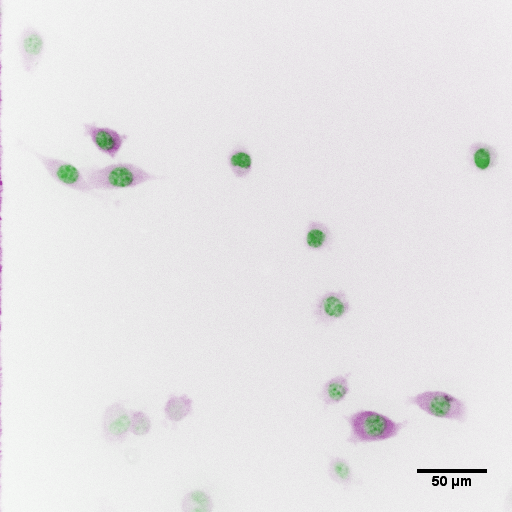
\includegraphics[scale=0.25]{Figures/Myocytes_impress.png} 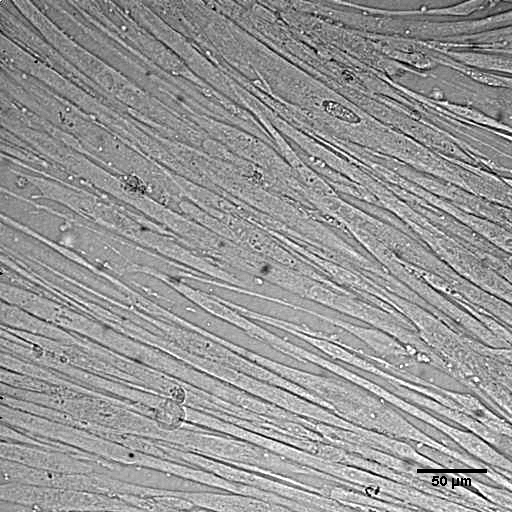
\includegraphics[scale=0.25]{Figures/Myotubes_flox_D4.png} 
\caption{Myoblastes primaires infectés avec un plasmide MRTF-A GFP, et myotubes obtenus à partir de myoblastes primaires après 4 jours de différenciation \textit{in vitro} par Alessandra Pincini. En vert, le noyau marqué au DAPI, en magenta MRTF-A GFP.}
\end{figure}


Les myoblastes sont les cellules progénitrices du muscle. Les C2C12 sont une lignée immortalisée de myoblastes murins, mais des myoblastes primaires peuvent également être mis en cultures \textit{in vitro}.
La différenciation se produit quand les myoblastes sont suffisamment nombreux et que les facteurs de croissance qui les maintiennent en prolifération viennent à manquer. 
%Les myoblastes se mettent alors à sécréter de la fibronectine, la liaison intégrine/fibronectine étant indispensable à la différenciation. 
%% Impossible de retrouver la référence
\begin{figure}
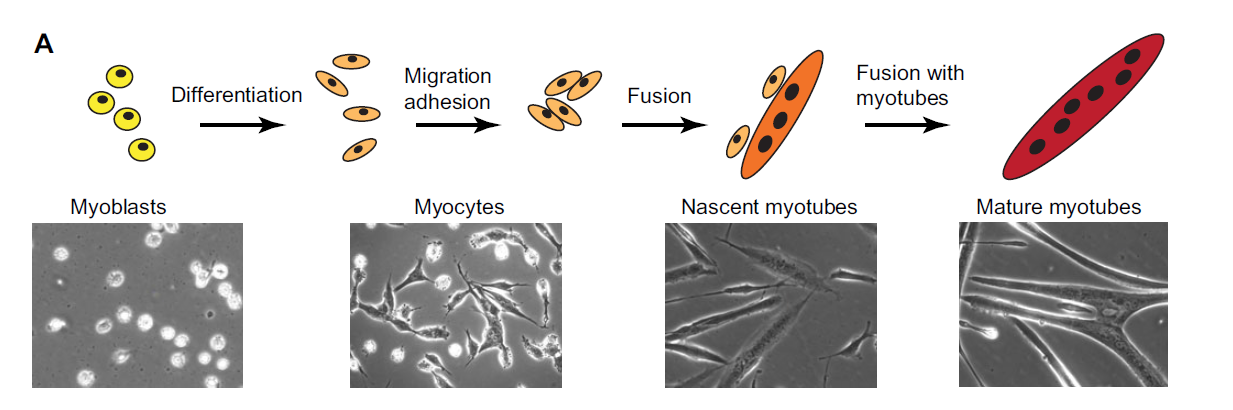
\includegraphics[scale=0.4]{Figures/Myoblast_fusion.png} 
\caption{\'Etapes successives de la différenciation des myoblastes en myotubes chez la souris, d'après \cite{abmayr_myoblast_2012}. }
\end{figure}

Les myoblastes vont alors s'aligner les uns avec les autres, sortir du cycle cellulaire et devenir des myocytes. Certains de ces myocytes deviendront des cellules fondatrices de myotubes. Les autres myocytes vont alors fusionner avec eux lors d'un processus asymétrique qui mène à la formation de myotubes polynuclés de plusieurs centaines de microns de long. 
Les myoblastes étendent autour d'eux des lamellipodes et des filopodes pour contacter les cellules voisines. Au niveau de ces contacts, les compositions en lipides de la membrane change, on trouve un grand nombre de protéines comme les M- et N-cadhérines, les intégrines et les filamines qui assurent un lien avec le cytosquelette (revue par \cite{abmayr_myoblast_2012}). Ce dernier est réorganisé localement : un réseau dense se forme sous la membrane, mis sous tension par la myosine 2A (\cite{duan_dependence_2009}). 
Le myoblaste envahit le myotube à l'aide de structures podosome-like quasiment exclusivement composées d'actine en filaments, avant que des pores se forment entre les deux cellules pour achever la fusion. 


\begin{figure}
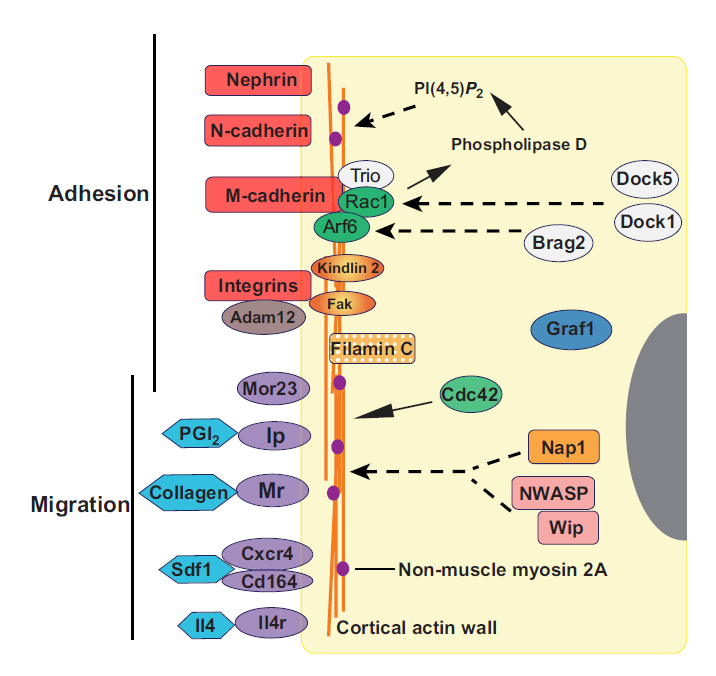
\includegraphics[scale=0.5]{Figures/Myoblast_pathways.png} 
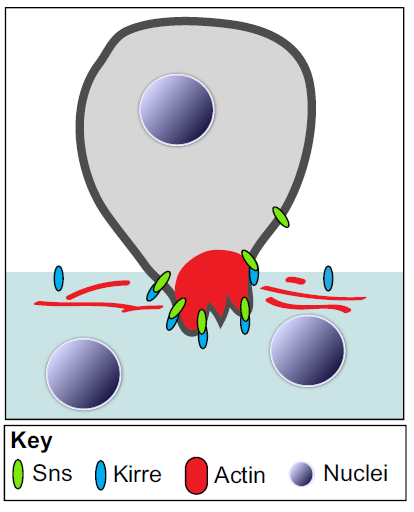
\includegraphics[scale=0.5]{Figures/Myoblast_invasion.png} 
\caption{Protéines impliquées dans la différenciation des myoblastes et invasion d'un myotube par un myocyte avant la fusion.}
\end{figure}

Une fois le myotube formé, il mature pour devenir une myofibre en développant une organisation spécifique de l'actine et de la myosine.




\subsection{Une organisation spécifique de l'actine et de la myosine }

À l'intérieur d'une myofibre totalement différenciée, l'actine est organisée en unités appelées les sarcomères. 

\begin{figure}[p]
\includegraphics[scale=0.2]{Figures/sarcomere.png} 
\caption{Organisation schématique du disque Z, d'après \cite{ferrer_molecular_2008}}
\end{figure}

Un sarcomère est composé de filaments d'actine et de filaments de myosines qui sont dotés de milliers de têtes de myosines. Le mouvement des têtes de myosines sur le filament d'actine fait coulisser les deux filaments l'un par rapport à l'autre, ce qui crée la contraction musculaire. 

Afin que les filaments d'actine, dont nous avons vu au chapitre 2 qu'ils sont ordinairement très dynamiques, maintiennent leur taille, ils sont coiffés aux deux extrémités par CapZ d'un côté et par la tropomoduline de l'autre.
On pense que les nébulines, de très longues protéines qui peuvent se lier à environ 200 actines en filament, servent d'étalon pour fixer la longueur des filaments d'actine dans les sarcomères. 



\begin{figure}[p]
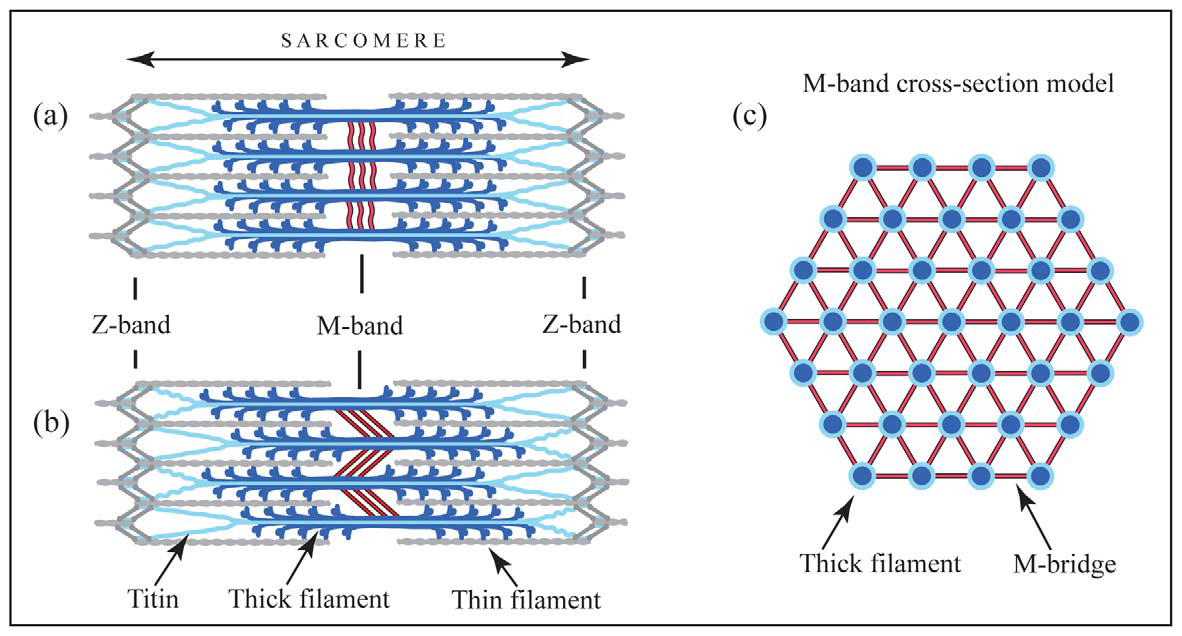
\includegraphics[scale=0.4]{Figures/Myomesine.png}
\caption{Organisation dans les deux plans des filaments de myosine au niveau de la bande M, d'après \cite{tskhovrebova_making_2012}}
\end{figure}
 
Autour des filaments d'actine, la tropomyosine, liée également à la troponine, régule la liaison entre le filament d'actine et le filament de myosine, en recouvrant ou découvrant les sites de liaison des têtes de myosines à l'actine, et le maintient polymérisé. 

Les filaments de myosine sont maintenus alignés grâce à la structure de la bande M, et les filaments d'actine par le disque Z. 

Au niveau de la bande M, les filaments de myosine se lient aux protéines M, aux myomésines et aux titines. 
La titine est une protéine géante qui maintient l'intégrité du sarcomère en se liant à la bande M, au disque Z et aux filaments de myosine. Elle présente une structure enroulée sur elle-même, et fonctionne comme un ressort qui stocke de l'énergie quand le sarcomère change de longueur, et contribue ainsi à maintenir l'intégrité de l'ensemble de la structure. 
Les myomésines ont une structure semblable mais sont plus courtes. Elles forment des ponts entre les filaments de myosines pour les maintenir dans une structure qui ressemble à un réseau hexagonal. 

Au niveau du disque Z, un grand nombre de protéines viennent assurer l'ancrage des filaments d'actine et l'organisation du sarcomère. Une partie d'entre elles est également partie prenante de cascades de signalisation.
L'$\alpha$-actinine, déjà évoquée précédemment en tant que protéine liée à l'actine, assure vis-à-vis de l'actine la même mission que les myomésines pour les filaments de myosine : elle lie les filaments entre eux pour former un réseau hexagonal, et lie également les titines. 
Par l'intermédiaire de la filamine C, l'$\alpha$-actinine relie les filaments d'actine du sarcomère aux intégrines qui assurent l'ancrage avec la matrice extra-cellulaire. 
La desmine, le filament intermédiaire du cytosquelette spécifique du muscle s'enroule autour du disque Z pour maintenir sa structure, et l'$\alpha$B-cristalline l'empêche de former des agrégats. 


\subsection{Rôle de la voie RhoA/MRTF-A/SRF}

Parmi les gènes cibles de SRF, on trouve un grand nombre de protéines indispensables à la constitution des sarcomères :  tous les différents gènes d'actine et en particulier l'$\alpha$ Skeletal Actin , des myosines (MHC9,myo16,myoIE), des $\alpha$-actinines, des intégrines et des tropomyosines (\cite{selvaraj_megakaryoblastic_2003},\cite{charvet_new_2006},\cite{esnault_rho-actin_2014}).

MyoD, facteur de transcription de la famille des Myogenic Regulatory Factors et marqueur de la différenciation en cellule musculaire, contient un Serum Response Element (\cite{lhonore_myod_2003}) et est activé par MRTF-A/SRF (\cite{mokalled_mastr_2012}). 

Il suffit qu'un seul des maillons de la voie RhoA/MRTF/SRF manque pour que la différenciation en cellule musculaire échoue. 

\textit{In vivo} dans des souris ayant une délétion conditionnelle de SRF dans les muscles, on observe une diminution de l'expression de la tropomyosine et de l'$\alpha$ actine du muscle squelettique, corrélés à des défauts dans la croissance des myofibres, une désorganisation des sarcomères et une hypotrophie musculaire (\cite{charvet_new_2006},\cite{li_requirement_2005}). 

Les souris dominant négatif MRTF-A sont viables mais présentent une hypotrophie musculaire qui dépend du niveau d'expression de MRTF-A, une fibrose, et des noyaux positionnés au centre des fibres musculaires, ce qui les désorganise \parencite{li_requirement_2005}. \textit{In vitro}, la différenciation des C2C12 nécessite également la présence des MRTF \parencite{selvaraj_megakaryoblastic_2003}, de SRF et de RhoA (\cite{wei_rhoa_1998}). 

\cite{kawauchi_p130cas-dependent_2012} détaillent un peu plus ces voies de signalisation impliquées dans la différenciation musculaire, en montrant que la signalisation passe par p130Cas, les intégrines $\beta$3 et ILK, qui désactivent à la fois ERK1/2 (ce qui empêche la phosphorylation de MRTF-A et donc promeut son accumulation nucléaire, et met hors-jeu les TCF), et la cofiline (ce qui promeut l'actine polymérisée). Ils montrent que p130Cas contribue à maintenir l'actine polymérisée et MRTF-A présent dans le noyau alors que la différenciation se fait dans un milieu pauvre en sérum, où RhoA est diminué. 
 
\subsection{De la fibre au muscle}

Les sarcomères mis bout à bout  forment des myofibrilles. Les myofibrilles adjacentes sont liées et alignées au niveau de leurs disques Z, afin que les contractions se fassent de manière synchronisée. 

\begin{figure}
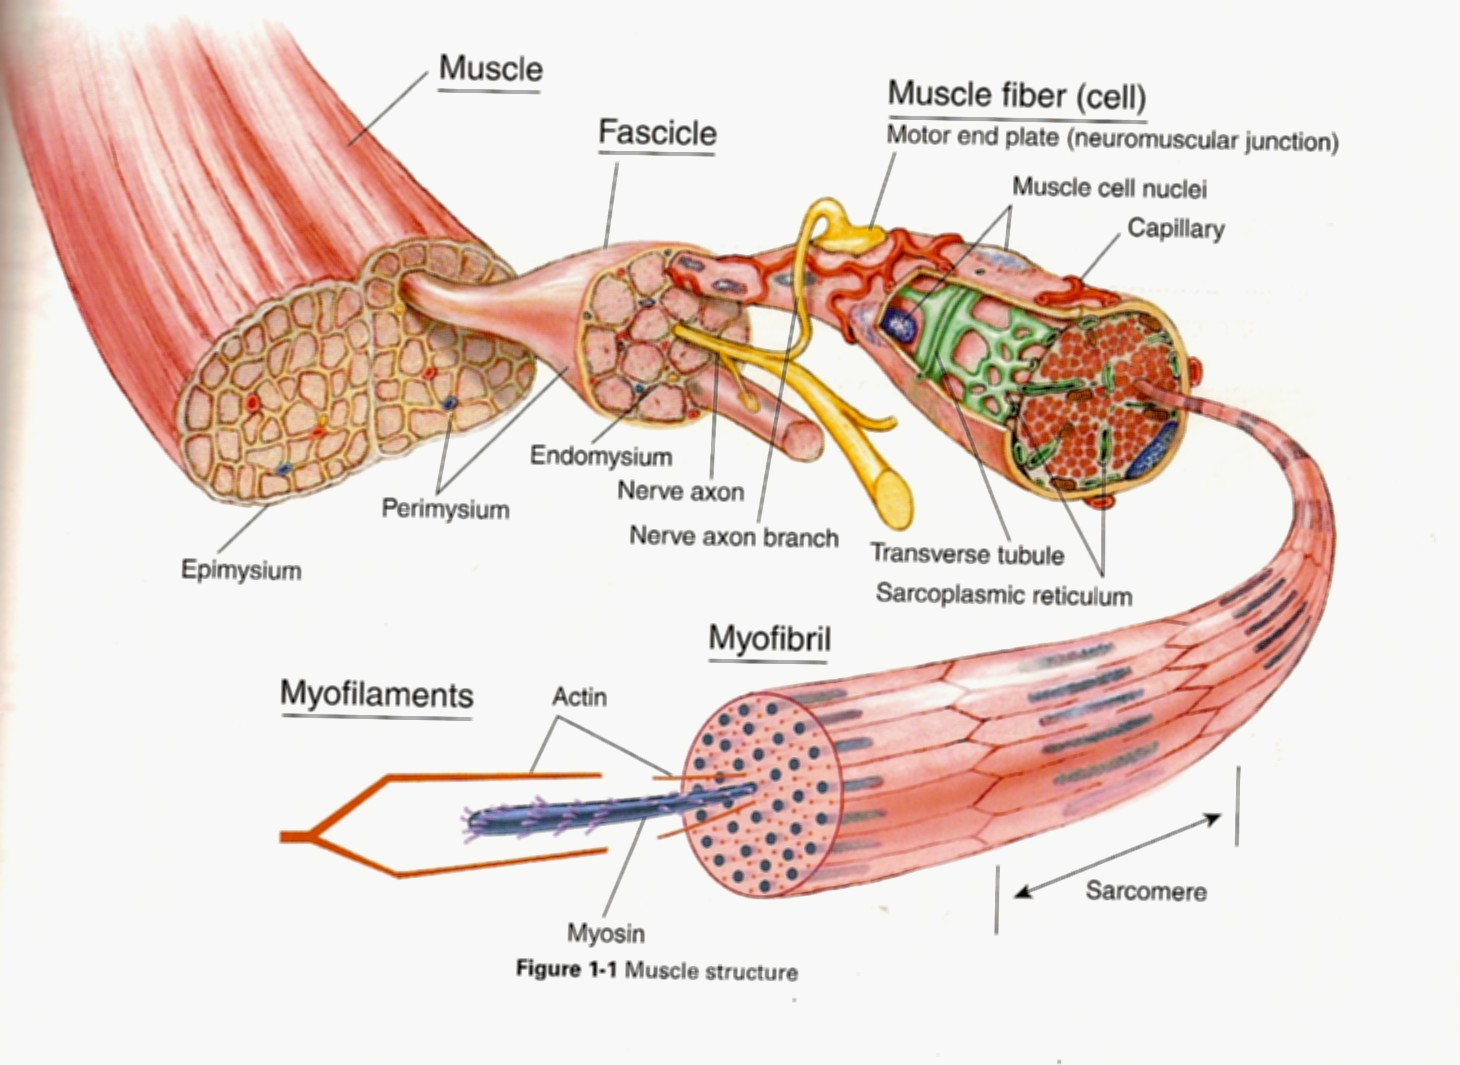
\includegraphics[scale=0.5]{Figures/12_29_0.png} 
 \caption{Illustration de la structure globale du muscle.}
\end{figure}

Dans une myofibre, on trouve de nombreuses myofibrilles liées les unes aux autres, de l'ordre de quelques dizaines, qui occupent la majeure partie de l'espace disponible. Les multiples noyaux sont repoussés en périphérie de la cellule. 

Les myofibres sont regroupées en faisceaux de quelques dizaines de fibres dans un tissu conjonctif composé principalement de différents types de collagène, faisceaux qui sont eux-même regroupés pour former le muscle lui-même. Le tissu conjonctif confère une résistance passive aux muscles et les relie aux tendons qui les fixent sur les os. 

Les capillaires sanguins et les nerfs contrôlant les contractions musculaires sont également encapsulés dans ce tissu conjonctif. 
\subsubsection{Différents types de muscles}

Les fibres musculaires ont toutes une organisation similaire, mais ne sont pas toutes identiques. 
On peut distinguer 2 types majeurs de fibres musculaires : les fibres lentes et les fibres rapides. Les fibres rapides sont mobilisées en premier mais sont plus fatigables que les fibres lentes.  

Les fibres lentes servent aux efforts de longue durée et de faible force, comme par exemple le maintien de la posture, elles se contractent lentement. 
Elles sont riches en mitochondries et en capillaires sanguins, car leur alimentation en énergie se fait principalement par la consommation d'oxygène. 
Les fibres rapides permettent des mouvements puissants, développant une grande force. Elles sont riches en glycogène, dont elles tirent la majeure partie de leur énergie. 





\section{La contraction musculaire}

\subsection{Mécanismes moléculaires}

Le signal de contraction musculaire arrive du système nerveux par un neurone moteur, qui est attaché à une fibre musculaire par la plaque motrice.
Lorsque le signal nerveux est transmis au niveau de la synapse, la membrane de la myofibre est dépolarisée, ce qui aboutit à libérer des ions calcium du Réticulum Sarcoplasmique (l'équivalent pour la cellule musculaire du Réticulum Endoplasmique lisse). 

Les ions calcium libérés se lient à la troponine C, qui est présente sur la tropomyosine qui décore les filaments d'actine dans le sarcomère. La tropomyosine est déplacée sur le filament d'actine, laissant apparaître les sites de liaison à la myosine, qui étaient cachés. 

Les têtes de myosine s'attachent au filament d'actine, puis l'ATP qu'elles contiennent est hydrolysée en ADP+Pi. Le phosphate est ensuite libéré, ce qui provoque un changement de conformation de la tête de myosine, qui avance sur le filament, puis l'ADP est relâchée à son tour, ce qui incline encore plus la tête de myosine. 

À ce moment, les filaments d'actine et les filaments de myosine coulissent les uns par rapport aux autres, ce qui raccourcit la longueur totale du sarcomère. C'est la contraction musculaire. 

En l'absence d'ATP, le phénomène s'arrête à cette étape : les filaments d'actine et de myosine sont attachés les uns aux autres. Le muscle est immobilisé, c'est l'origine de la rigidité cadavérique. 

Lorsqu'elle est présente, l'ATP peut alors remplir le site de liaison laissé vacant par le départ de l'ADP. Cela provoque à nouveau un changement de conformation qui détache la tête de myosine du filament d'actine et la remet dans sa position initiale.

Tant que la concentration en ions calcium est suffisante pour maintenir la tropomyosine dans cette configuration, le cycle attachement-avancée-détachement des têtes de myosine sur l'actine continue, et la fibre musculaire se contracte de plus en plus. 

Lorsque la concentration en calcium diminue car le signal du neurone moteur s'est arrêté, la tropomyosine retrouve sa conformation d'origine, et les myosines ne peuvent plus s'attacher au filament d'actine. 

Pendant la contraction, les protéines du disque M, du disque Z et la titine, qui maintiennent l'alignement des filaments d'actine et de myosine, ont été étirées. Ces protéines peuvent être dépliées pendant la contraction et stocker de l'énergie élastique qui sera rendue lorsque les têtes de myosine seront détachées des filaments d'actine. Lorsque la contraction s'arrête, les filaments coulissent à nouveau dans l'autre sens sous l'action de l'élasticité de ces protéines, et le sarcomère  reprend sa longueur initiale. 


\begin{figure}[p]
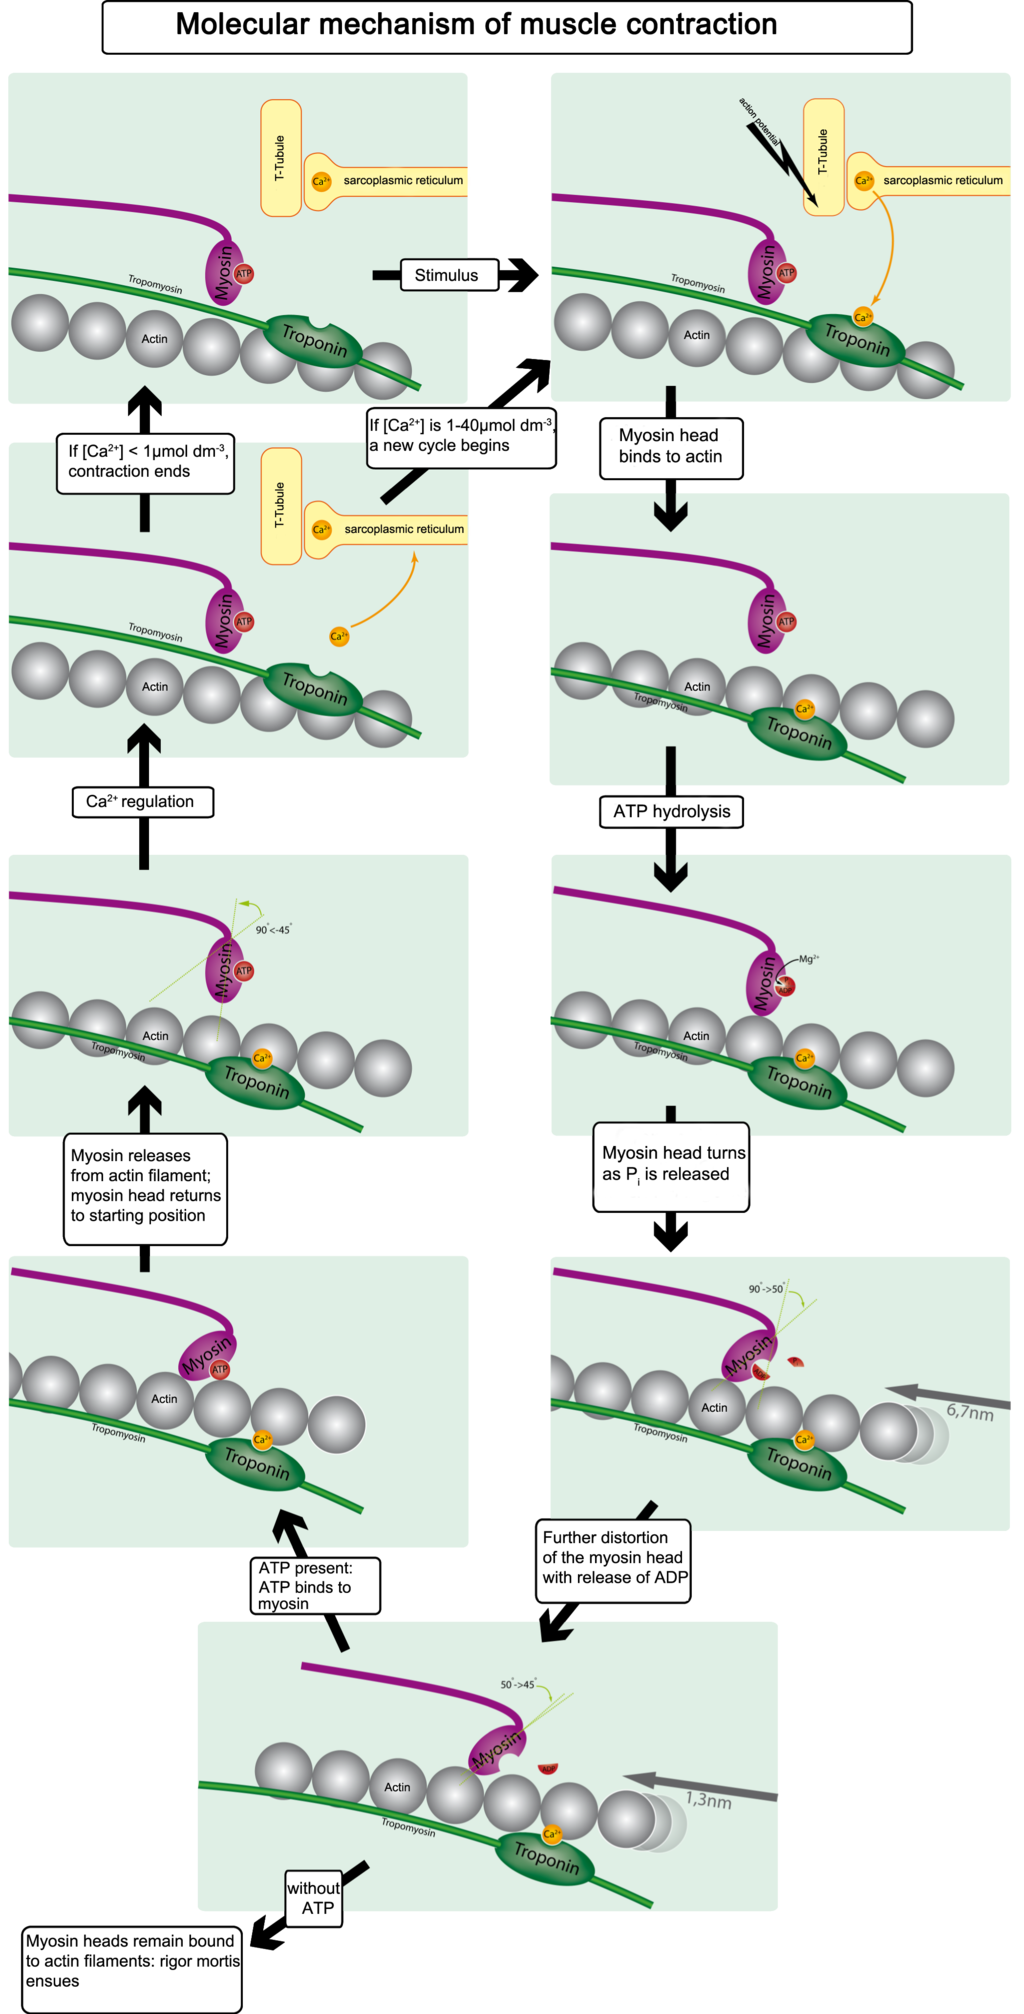
\includegraphics[scale=0.25]{Figures/Contraction.png}
\caption{Illustration du cycle de la contraction musculaire, réalisée par Hank van Helvete (CC BY-SA 2.5)}
\end{figure}
\subsection{Mécanique de la contraction musculaire}
Dans les conditions optimales, une seule cellule musculaire mature humaine peut exercer une force de l'ordre de 0,3 \micro N, et un muscle peut exercer autour de 30N par cm$^2$ de section. 

Le modèle de Hill (\cite{hill_heat_1938}), élaboré bien avant que les mécanismes internes de la contraction musculaire soient connus, permet de relier la vitesse de contraction d'un muscle aux forces qu'il est capable de développer. 

Hill constate que pour un muscle de taille donnée se raccourcissant d'une longueur $x$, l'énergie dissipée dans le muscle est proportionnelle à $x$ : $W_d=ax$. $a$ est proportionnel à la section du muscle (et donc au nombre de myofibres), et comme la force maximale $ P_0$ supportée par le muscle également, le rapport entre les deux  est constant : $$\frac{a}{P_0}=0.25$$

En faisant un bilan d'énergie dans le muscle, on obtient : 
$$ E=W+W_d=Px+ax=(P+0.25P_0)x$$

La puissance totale dissipée vaut alors $(P+a)v$ où $v$ est la vitesse de contraction du muscle, dérivée de $x$ par rapport au temps. 

Hill trouve également que la puissance développée par le muscle est une fonction linéaire du poids qui lui est appliqué, avec $v=0$ quand $P=P_0$. 
La relation devient alors : 
$$ (P+a)v=b(P_0-P)$$
avec $b$ une constante mesurée dans les expériences. 

Cette relation peut se réécrire : 
\begin{equation}
\label{Hill}
(P+a)(v+b)=b(P_0+a)=Cste
\end{equation}
L'équation de Hill relie donc la force que peut appliquer un muscle $P$ à la vitesse de contraction $v$. Plus la contraction est rapide, moins elle peut être forte, au contraire plus elle est lente et plus elle peut développer de force. 

Non seulement la loi de Hill est vérifiée pour les muscles striées, mais elle l'est également au niveau du myoblaste unique (\cite{mitrossilis_single-cell_2009}) et même au niveau d'un unique filament d'actine déplacé par 8 têtes de myosine du muscle squelettique (\cite{debold_slip_2005}), ce qui confirme l'hypothèse de Huxley qui attribue ce comportement aux propriétés du complexe acto-myosine. 

\section{Les cellules satellites, MRTF-A et régulation de la masse musculaire}

Le muscle est un tissu plastique : il peut augmenter ou diminuer sa masse en réponse aux sollicitations mécaniques qui lui sont imposées. Nous en faisons tous quotidiennement l'expérience : la pratique d'activités physiques augmentent la taille de nos muscles, tandis qu'une immobilisation prolongée, comme par exemple suite à une fracture, conduit à une diminution rapide de notre masse musculaire. L'équipe d'Athanassia Sotiropoulos à l'Institut Cochin, avec laquelle nous avons collaboré, a caractérisé le rôle central de SRF dans ce phénomène. 

Entre la lame basale et les myofibres, on peut trouver des cellules satellites, qui contrairement aux autres cellules présentes dans le muscle, sont moins engagées sur la voie de différenciation et peuvent toujours proliférer. Les myoblastes C2C12 et primaires sont issues des cellules satellites prélevées sur des souris. Les cellules satellites sont responsables de la réparation et de la croissance des muscles adultes. 
En effet, les myofibres sont des cellules qui ne se reproduisent plus, et après les deux phases de création de myofibres pendant la vie embryonnaire, le nombre de fibres musculaires reste constant. 
Cependant, lorsqu'elles sont activées en réponse à une blessure ou à une sollicitation importante du muscle, les cellules satellites prolifèrent, et une partie d'entre elles se différencient et fusionnent avec les fibres musculaires. 

Pour étudier la réponse à une stimulation mécanique, des souris ont été soumises à une hypertrophie compensatoire : un des muscles de la patte ne peut plus faire son travail (parce qu’il est dénervé ou que le tendon est sectionné), et les autres sont obligés de compenser son manque d'activité en développant plus de force. En réponse à cette surcharge de travail, SRF est activé dans les myofibres \textit{in vivo} par l'intermédiaire de MRTF-A  (\cite{guerci_srf-dependent_2012}). 
L'activation de SRF dans les myofibres produit un signal paracrine composé d'Interleukines 6, qui encourage la prolifération des cellules satellites, et d'interleukines 4 qui les fait fusionner avec les fibres musculaires. 
Dans les fibres musculaires mutantes où SRF est désactivé, le nombre de noyaux par fibre n'augmente pas, ce qui signifie qu'il n'y a pas de fusion des cellules satellites avec les myofibres. La surexpression d'IL6 chez les mutants restaure la prolifération, mais pas la fusion des cellules satellites. Surexprimer IL4 ou Cox2, qui est en aval de SRF et en amont de l'IL4, permet de restaurer la fusion et l'hypertrophie chez les mutants. 


Au contraire, lors d'une absence de signaux mécaniques induite par la dénervation, l'actine G s'accumule dans le noyau des fibres musculaires et l'activité de SRF diminue (\cite{collard_nuclear_2014}). Le rôle de MICAL-2 est normalement d'exclure l'actine du noyau, et son activité est réduite pendant l'atrophie, ce qui contribue donc à l'accumulation nucléaire d'actine constatée. 
L'accumulation d'actine G dans le noyau favorise l'export de MRTF-A, qui est confiné dans le cytoplasme dans les muscles dénervés. Cela explique le déficit d'activité de SRF, qui ne peut pas être atteint par son cofacteur. 

La désactivation de SRF, l'injection de CCG1423 (drogue inhibant MRTF/SRF), ou l'expression d'une actine non polymérisable conduisent tous à une aggravation de l'atrophie musculaire, ce qui montre que cette voie de signalisation protège l'organisme de la destruction de ses propres muscles. 

Au contraire, l'expression d'une MRTF-A incapable de se lier à l'actine, et donc constitutivement active (sur le modèle de la myocardine), permet de protéger les muscles de l'atrophie induite par la dénervation, ce que ne fait pas la simple sur-expression de MRTF-A GFP. Cependant, si SRF n'est pas fonctionnel, cette protection n'est plus efficace, ce qui prouve que c'est bien le couple MRTF/SRF qui est nécessaire. 


%\end{document}



%\documentclass{report}
%\usepackage[T1]{fontenc}
%\usepackage[utf8]{inputenc}
%\usepackage[francais]{babel}
%\usepackage{amsmath}
%\usepackage{graphicx}
%\graphicspath{{Figures/}}
%\usepackage[backend=biber,style=authoryear,bibencoding=utf8]{biblatex}
%\usepackage[colorlinks,linkcolor=blue]{hyperref}
%\newcommand{\micro}{$\mathrm{\mu}$}
%\addbibresource{biblio2.bib}
%
%\begin{document}

\chapter{Rhéologie cellulaire}
\begin{center}

\includegraphics[scale=0.7]{Chapitre5.png}

\end{center}
\newpage

L'étude des propriétés mécaniques des objets biologiques (cellules, tissus, gels de biopolymères \dots) a été étudiée par des physiciens convergeant à la fois de la mécanique des milieux continus, de la physique de la matière molle (polymères, mousses, colloïdes, verres), et de l'hydrodynamique. 
En effet, ils rassemblent des objets et des propriétés qui intéressent tous ces domaines, d'une échelle moléculaire à une échelle macroscopique. 

Il est aisé de voir à quel point la mécanique peut être un aspect important du vivant : les médecins détectent les anomalies d'un tissu en testant sa rigidité \og à la main \fg pendant une palpation, l'absence de gravité a des conséquences importantes sur les os, et l'absence d'exercice sur les muscles, tandis que les changements de propriétés mécaniques des globules rouges ou des parois des vaisseaux sanguins peuvent se révéler dramatiques. 

Les matériaux vivants, comme les tendons, les os ou la cornée, ou issus du vivant comme la soie ou la nacre, peuvent également posséder des propriétés rhéologiques intéressantes, que l'on cherche à dupliquer pour créer de nouveaux matériaux composites. 

Les matériaux vivants combinent plusieurs particularités qui en font des objets particulièrement difficiles à étudier du point de vue physique : ils sont intrinsèquement hors de l'équilibre thermodynamique, car ils consomment de l'énergie en permanence, ils ne sont le plus souvent ni homogènes, ni isotropes, sont composés d'une grande diversité de constituants différents, leurs propriétés varient à la fois au cours du temps et d'un individu à l'autre. 
Tous ces éléments rendent plus complexes la reproductibilité d'une mesure à l'autre, la comparaison de mesures prises par des techniques différentes, l'élaboration de modèles théoriques et de simulations numériques.


\section{Rhéologie}

La rhéologie est l'étude de la manière dont les matériaux se comportent lorsqu'ils sont soumis à une contrainte mécanique.

Par exemple, on appelle solide élastique un matériau pour lequel la déformation $\epsilon$ est proportionnelle à la contrainte $ \sigma$. On appelle module d'Young ce coefficient de proportionnalité quand on applique un étirement uniaxial (voir figure \ref{young}): 
$$ E = \frac{\sigma}{\epsilon}$$
La déformation élastique est parfaitement réversible, c'est-à-dire que si on enlève la contrainte, le matériau revient à sa forme initiale. C'est le cas, aux petites déformations, de solides comme l'acier, le verre, le caoutchouc etc. Au niveau énergétique, la déformation élastique est donc une manière de stocker de l'énergie dans le système par l'intermédiaire de la déformation, énergie qui pourra être récupérée plus tard lorsque le solide reprendra sa forme initiale. 

\begin{figure}
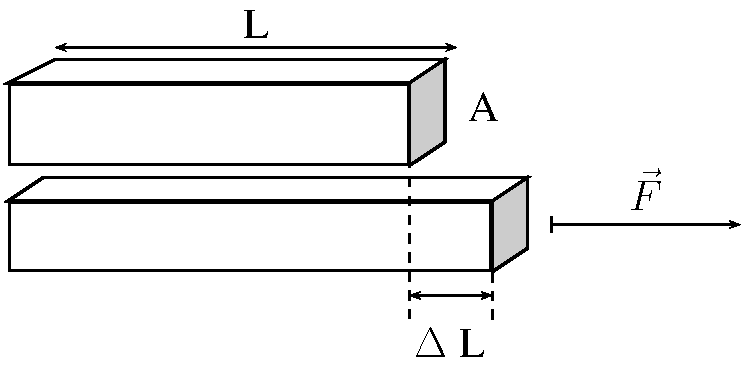
\includegraphics[scale=0.5]{Figures/Young_modulus.pdf} 
\caption{Solide élastique de section $A$ soumis à une contrainte $\sigma=\frac{F}{A}$ et déformé de $\epsilon=\frac{\Delta L}{L}$. \label{young} }
\end{figure}

Au contraire, pour les liquides visqueux, la viscosité $\eta$ représente la relation entre la contrainte et le taux de déformation $\dot{\epsilon}$ : 
$$ \eta=\frac{\sigma}{\dot{\epsilon}}$$
Le liquide va donc être déformé de manière linéaire au cours du temps sous l'effet d'une contrainte constante. Lorsque la contrainte est levée, la déformation s'arrête, mais le liquide ne reprend pas la forme qu'il avait avant son application. 
L'écoulement visqueux est un phénomène irréversible, et l'énergie qui a été fournie pour le faire s'écouler est dissipée. 

Le liquide purement visqueux et le solide purement élastique sont des modèles qui ne sont valables que dans certaines limites. Une barre d'acier est élastique dans une gamme de contraintes et de déformations, au-delà elle est plastique : elle se déforme de manière irréversible en réponse à la contrainte. 
Cela peut également dépendre de l'échelle de temps à laquelle on se place, par exemple, le manteau de la croûte terrestre peut être considéré comme un solide élastique à une échelle de temps de quelques heures, mais à des échelles de temps géologiques, il peut être considéré comme un liquide extrêmement visqueux ($\eta \approx 10^{21}$Pa.s). 


La fonction de fluage quantifie la déformation d'un matériau en réponse à une contrainte $\sigma$ constante appliquée à partir d'un temps $t=0$. 
Dans le cas simple du solide élastique, la fonction de fluage est une constante : à l'application d'une contrainte, le matériau est immédiatement déformé, et cette déformation reste constante par la suite. Par exemple, dans le cas d'un étirement uniaxial : 
$$J(t)=\frac{1}{E}$$
Dans le cas d'un liquide visqueux cisaillé, la fonction de fluage est une fonction linéaire du temps : 
$$ J(t)=\frac{t}{\eta}$$

Les cellules vivantes et la plupart des bio-polymères sont des matériaux visco-élastiques, ce qui signifie qu'une partie de l'énergie transmise par la contrainte va être stockée, et une autre va être dissipée. Il existe plusieurs manières simples de combiner les deux modèles précédents pour créer un modèle de visco-élasticité. 

Les deux plus simples sont le modèle de Kelvin-Voigt et le modèle de Maxwell, qui associent un élément élastique de module d'Young $E$ et un élément visqueux de viscosité $\eta$, le premier en parallèle et le second en série. 
Dans le modèle de Maxwell, lorsque l'on impose une contrainte $\sigma$ constante, on obtient une superposition des deux fonctions de fluage précédentes : 
$$J(t)=\frac{1}{E} + \frac{t}{\eta} = \frac{1}{E} \left( 1 + \frac{t}{\tau} \right) \qquad \tau= \frac{\eta}{E}$$ 
et donc une déformation affine au cours du temps. Le matériau se déforme de manière élastique, puis coule en relaxant la contrainte. 
Dans le modèle de Kelvin-Voigt : 
$$ J(t)=\frac{1}{E} e^{-\frac{t}{\tau}} \qquad \tau=\frac{\eta}{E}$$
Un temps caractéristique du système apparaît, en dessous duquel la réponse est principalement élastique, et au-dessus duquel la déformation est principalement visqueuse. 

Ces deux modèles peuvent être ensuite complexifiés, en combinant plusieurs éléments visqueux et plusieurs éléments élastiques, en parallèle et/ou en série. 

Lorsque la sollicitation mécanique n'est plus une contrainte constante, mais sinusoïdale de fréquence $\omega$, on parle plutôt en terme de module visco-élastique : 
$$G(\omega) = \frac{\sigma(\omega)}{\epsilon(\omega)} = G'(\omega)+iG''(\omega)$$

$G'$ est le module de stockage, et correspond à la part élastique de la réponse, tandis que $G''$ est le module de perte, qui quantifie la dissipation. Pour un solide élastique on a $G'=E$ et $G''=0$, alors que pour un liquide visqueux $G'=0$ et $G''=\omega \eta$. 

Pour un modèle de Kelvin-Voigt : 
$$ G=E+ i \omega \eta$$
et pour un fluide de Maxwell : 
$$ \frac{1}{G} = \frac{1}{E} + \frac{1}{i \eta \omega}$$


\section{Propriétés des réseaux d'actine in vitro}

Une des approches utilisées par les physiciens pour aborder l'étude des objets biologiques consiste à rechercher le système le plus simple pour lequel les propriétés observées dans le vivant peuvent être reproduites. 
En partant d'un très petit nombre de protéines purifiées, re-mélangées \textit{in vitro}, on peut reconstruire des modèles simplifiés du cytosquelette, dans le but de comprendre quels éléments, et quelles associations d'éléments sont à l'origine des propriétés des cellules. 

Dans le cas de l'actine, cela peut être un gel d'actine purifiée, auquel on peut ajouter des protéines réticulantes, comme l'$\alpha$-actinine, la scruine ou la filamine, des moteurs moléculaires comme les myosines ou Arp2/3 pour créer des réseaux branchés. 

Les gels d'actine ont des modules d'Young allant typiquement de 1 à plusieurs centaines de Pascal pour 2mg/ml d'actine purifiée, les valeurs dépendant beaucoup de la qualité de purification des protéines et du degré de polymérisation des filaments (\cite{janmey_mechanical_1994}). Par exemple, l'ajout de gelsoline pour dépolymériser les filaments fait chuter les valeurs à moins 1Pa. 

Les gels d'actine purifiée concentrée et polymérisée, même en l'absence de tout réticulant se rigidifient sous contrainte. Deux mécanismes principaux expliquent ce comportement. 
D'une part, les filaments d'actine semi-flexibles, lorsqu'ils sont étirés, perdent des degrés de liberté de fluctuation, et cela crée une élasticité entropique (\cite{storm_nonlinear_2005}). Plus la contrainte et grande, et plus les possibilités se réduisent, et plus le gel se rigidifie. 
D'autre part, les filaments sont semi-flexibles et ont donc une élasticité de courbure, qui a déjà été définie au chapitre 2, qui est une deuxième source de non linéarité. 

Au-delà d'une certaine déformation, par exemple 20\% pour des gels d'actine 2mg/ml soumis à un cisaillement, les gels d'actine cèdent, et leur module élastique diminue brutalement de manière irréversible (\cite{janmey_mechanical_1994}).
Il est à noter que les valeurs de modules élastiques mesurées pour les gels d'actine sont apparemment extrêmement dépendantes des conditions de purification, de stockage et de polymérisation de l'actine. 

L'ajout de réticulants permanents, comme la scruine, rend le gel quasiment exclusivement élastique, avec un module qui dépend principalement de la concentration en réticulants. 
Les réticulants dotés d'un temps caractéristique d'interaction entre deux filaments, comme l'$\alpha$-actinine ou la filamine, n'augmentent pas autant la rigidité des gels d'actine. 
La réponse en fréquence de ces mélanges est également modifiée par la cinétique d'interaction entre les filaments et les réticulants, car une molécule avec des temps de détachement courts permet plus de dissipation et de relaxation des contraintes qu'une protéine interagissant longtemps. 
Les gels réticulés ont un comportement encore plus non-linéaire que les gels d'actine simple, allant jusqu'à des rigidités multipliées par 100 pour des gels avec de la filamine \parencite{gardel_stress-dependent_2006}. 

L'ajout de moteurs dans le réseau d'actine est encore une question de physique tout à fait différente. En plus de lier les filaments entre eux à la manière d'un réticulant classique, les myosines consomment de l'ATP et produisent des déplacements de filaments les uns par rapport aux autres, sans qu'il soit nécessaire de leur appliquer une contrainte extérieure. 
Un gel d'actine, de filamine et de myosine peut alors se rigidifier sans contrainte, uniquement sous l'action des moteurs moléculaires mettant en tension le réseau \parencite{koenderink_active_2009}. 
La consommation d'ATP par les myosines place également le gel hors de l'équilibre thermodynamique. 
Avec des concentrations d'ATP qui permettent aux myosines de faire coulisser les filaments les uns par rapport aux autres, le théorème fluctuation-dissipation n'est alors plus valable \parencite{mizuno_nonequilibrium_2007}, alors qu'il l'est sans ajout de myosines, ou lorsque la fréquence de stimulation est supérieure à 10 Hz. 



\section{Techniques de rhéologie cellulaire}

\begin{figure}
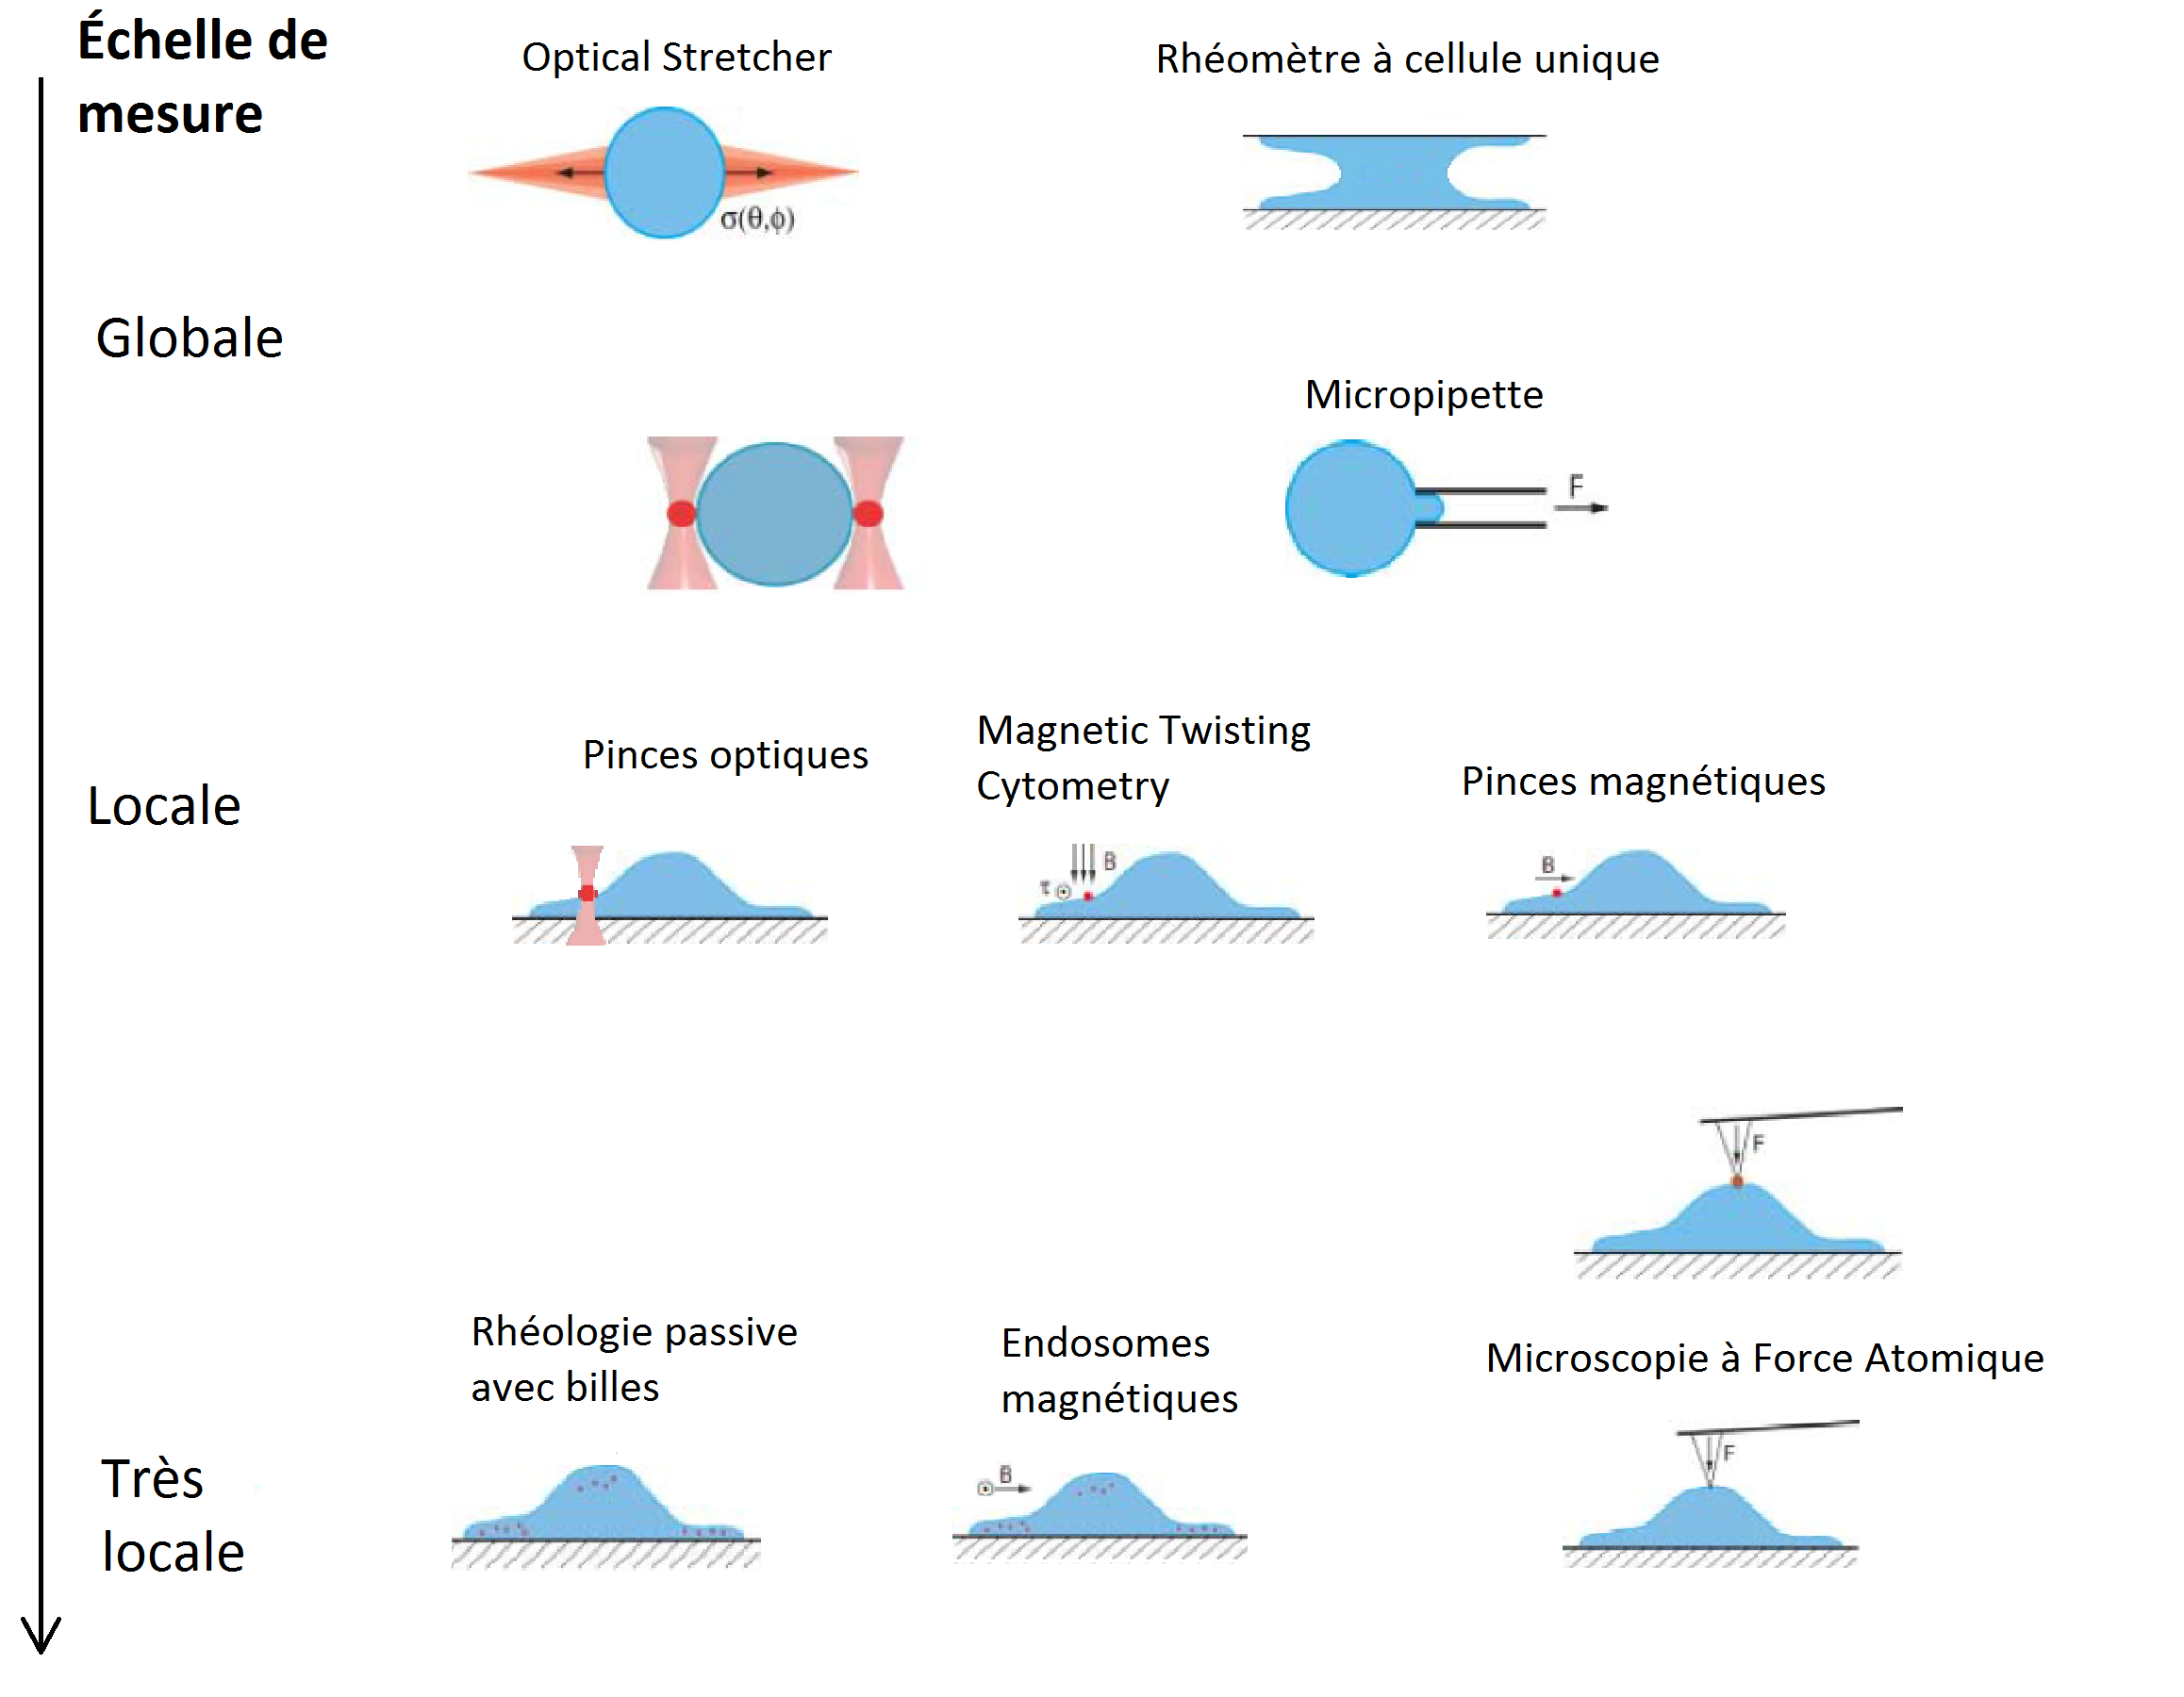
\includegraphics[scale=0.2]{Rheologie.png}
\caption{Principales techniques de rhéologie, classées en fonction de l'échelle de taille à laquelle elles sondent les cellules. Adapté de \cite{huber_emergent_2013}.}
\end{figure}

De très nombreuses techniques ont été développées pour sonder les propriétés mécaniques des cellules \textit{in vitro}, mais elles ne sondent pas toutes exactement la même chose. 

%AJOUTER UNE FIGURE, PRISE PAR EXEMPLE DANS UNE REVUE QUI LISTE LES DIFFERENTES TECHNIQUES.

En premier, les techniques peuvent être classées en deux catégories : les techniques de rhéologie active, où l'on applique une contrainte mécanique extérieure à la cellule, et les techniques de rhéologie passive, où il n'y a aucune contrainte ou déformation imposée. 

Les techniques se distinguent également par l'échelle à laquelle elles sondent les cellules : certaines techniques sont globales, comme la micropipette ou le rhéomètre à cellule unique, d'autres sont locales comme les pinces optiques, et même parfois très locales, comme l'AFM. 
Selon la taille caractéristique de l'élément sondé, ce ne sont pas les mêmes éléments du cytosquelette qui sont caractérisés : une technique sondant la réponse locale à la surface de la cellule verra principalement le cortex cellulaire, tandis qu'une bille enfoncée profondément au milieu du corps cellulaire verra le cytosquelette interne. 

Certaines techniques appliquent la contrainte par l'intermédiaire des protéines d'adhésion, ce qui est le cas de la majorité des techniques de billes par exemple, tandis que d'autres peuvent sonder directement la mécanique cellulaire, comme l'AFM ou l'étireur optique (optical stretcher). Cet aspect est particulièrement important pour étudier la mécanotransduction : savoir si le signal mécanique est médié ou non par les diverses adhésions à la matrice extra-cellulaire ou aux autres cellules est une information essentielle pour comprendre le phénomène. 
Cependant, la présence de ces adhésions oblige à faire des hypothèses sur les liaisons avec la cellule qui peuvent parfois affecter grandement les valeurs mesurées. 

Parmi les techniques de rhéologie active, certaines appliquent des contraintes à l'aide de force, d'autres à l'aide de couples, et d'autres encore imposent des déformations. Ces différences peuvent parfois rendre difficiles les comparaisons entre les résultats, lorsqu'il faut replacer les mesures sur une échelle commune à des techniques différentes. 

Dans chacune des deux principales catégories, les techniques seront présentées dans un ordre approximatif de la technique la plus globale à la plus locale. 

\subsection{Les techniques de rhéologie active}
\subsubsection{Les techniques globales}
Les techniques de rhéologie globales stimulent la cellule dans son entier, ou sur la majeure partie de son volume. Elles ont l'avantage de considérer les cellules comme un tout. 

\paragraph{Rhéomètre à cellule unique (Single Cell Rheometer)}

Le rhéomètre à cellule unique est composé de deux fines plaques de verre recouvertes de protéines d'adhésion entre lesquelles est placée une cellule. Une des lamelles est infiniment rigide par rapport à la cellule, l'autre est souple et va être défléchie. 
La déflexion de la lamelle souple est mesurée, soit directement sur l'image de microscopie, soit indépendamment, et permet de connaître ou de fixer la force appliquée aux cellules. 

Le dispositif est décrit en détail par \cite{desprat_creep_2005} et \cite{bufi_single-cell_2015}. 




Il peut appliquer une contrainte sinusoïdale ou constante, et donc mesurer le module visco-élastique $G(\omega)$ ou la fonction de fluage $J(t)$. 

Le dispositif applique des forces du nN à la centaine de nN.



\paragraph{Optical stretcher}

L'étireur optique se base sur le principe des pièges laser.
Lorsqu'un objet est piégé entre deux faisceaux laser gaussiens identiques venant de directions opposées, il est piégé et soumis à un étirement le long de l'axe des faisceaux. 
Les deux faisceaux doivent pour cela être légèrement plus grands que l'objet lui-même. 

Cette technique a été utilisée pour sonder la mécanique de cellules en suspension en observant leur déformation lorsqu'elles passent entre les deux faisceaux \parencite{guck_optical_2001}. 
Comme pour le rhéomètre à cellule unique, c'est la cellule dans sa globalité qui est testée, mais cette fois de manière totalement indépendante de l'adhésion. 

L'optical stretcher applique des forces de l'ordre de quelques pN. 

Cette technique sonde les cellules en l'absence de toute adhésion. Cela peut être un avantage dans le cas de cellules qui sont naturellement en suspension, comme les érythrocytes, mais pour des cellules naturellement adhérentes, cela pose la question de la pertinence des mesures faites dans des circonstances aussi inhabituelles pour elles. 

\paragraph{Micropipette}

L'utilisation de micropipettes est la technique la plus ancienne de rhéologie cellulaire (revue par \cite{hochmuth_micropipette_2000}). 
Dans sa version la plus simple, il s'agit d'aspirer tout ou partie de la cellule dans une micropipette avec une certaine dépression, et d'observer la déformation résultante. 
Lorsqu'une partie de la cellule est aspirée, ce sont la taille et la forme de la partie aspirée qui sont analysées pour remonter aux paramètres mécaniques. 
Cela peut être fait sur des cellules en suspension ou sur des cellules adhérentes.
Une autre méthode pour les cellules en suspension consiste à aspirer la cellule complètement dans la pipette, puis à la relâcher, et d'observer sa relaxation vers sa forme d'origine. 

 
%Avec deux micropipettes, il est également possible de sonder les interactions entre deux cellules. 

Cette technique permet d'exercer des forces de 10pN à la centaine de nN, ce qui en fait probablement la technique ayant le plus large éventail de possibilités. Sa résolution spatiale est en revanche limitée à des déformations qui sont grandes à l'échelle de la cellule. 



\subsubsection{Les techniques de billes}
Ces techniques utilisent des billes micrométriques recouvertes de protéines d'adhésion qui se lient aux récepteurs de la membrane et servent d'intermédiaire pour exercer des contraintes sur les cellules. 

Que la force soit appliquée sur la bille par un laser ou par un champ magnétique, le principe reste le même. La contrainte est transmise à la cellule par l'intermédiaire des protéines d'adhésion, ce qui signifie que les voies de mécanotransduction activées au niveau des adhésions vont également être stimulées. 
La stimulation est plus ou moins locale, selon le rapport entre la taille de la cellule et la taille de la surface de contact avec la bille.

Les estimations de modules visco-élastiques obtenues par des techniques de billes sont souvent très dépendantes des hypothèses qui sont faites sur la densité de liaisons au niveau de la surface de contact et du modèle mécanique qui permet d'obtenir une relation contrainte-déformation à partir de la relation entre la force exercée sur la bille et le déplacement de celle-ci. 
De plus, les billes sont plus ou moins enfoncées dans la cellule, selon les ligands, les types cellulaires, les temps d'incubation, et cela change la nature des éléments du cytosquelette qui vont être sondés : le cortex pour une bille en surface, le lamellipode pour une bille sur le bord en progression, le noyau pour une bille enfoncée au contact de celui-ci\dots


\paragraph{Magnétocytométrie}

Cette technique est la première des techniques de billes. Elle utilise des billes ferromagnétiques de taille micrométrique (de 3 à 4,5 \micro m), recouvertes de protéines d'adhésion, pour appliquer un couple sur les cellules \parencite{wang_mechanotransduction_1993}.

Les billes, préalablement magnétisées dans le plan du substrat, ancrées sur les cellules, sont soumises à un champ perpendiculaire à leur moment magnétique. En cherchant à s'aligner avec le champ, elles exercent un couple sur les cellules auxquelles elles sont ancrées. L'orientation moyenne des billes est alors mesurée par un magnétomètre. Les contraintes appliquées vont du Pascal à la centaine de Pascal. 

L'avantage et l'inconvénient de cette méthode sont qu'elle permet d'observer une grande population de cellules en même temps. Le champ résultant correspond à une moyenne de toutes les rotations de toutes les billes sur les cellules. Mais elle réduit également l'information à cette moyenne, et il n'est pas possible d'obtenir plus de détails sur les comportements à l'intérieur de la population : une population composée de cellules très molles qui laissent la bille s'aligner presque complètement et de cellules très rigides qui ne la laisse quasiment pas tourner pourra donner des résultats identiques à une population composée de cellules qui laissent la bille former un angle de 45\degres avec le champ. 

Une variante de cette technique consiste à observer le mouvement des billes avec un microscope pour en déduire la déformation de la cellule \parencite{fabry_scaling_2001}. Cela réduit le nombre de cellules observées, mais permet d'avoir plus d'informations sur la population que la simple moyenne. Cela permet également de mesurer le comportement fréquentiel, en appliquant un champ magnétique oscillant. 






\paragraph{Pinces magnétiques}

Le principe des pinces magnétiques est d'utiliser des billes de taille micrométrique qui contiennent des nanoparticules de fer qui les rendent super-paramagnétiques.
Ces billes soumises à un champ et à un gradient de champ magnétiques créé par un électro-aimant sont attirées vers lui avec une force qu'il faut calibrer à l'avance.
La force exercée sur une bille peut alors être réglée en modifiant le courant électrique parcourant l'électro-aimant.
Ces billes sont fonctionnalisées avec des protéines d'adhésion (fibronectine ou fragment de fibronetine, cadhérines, \dots), elles vont donc sonder le cytosquelette par l'intermédiaire de ces protéines. 


Les pinces magnétiques peuvent appliquer des forces de l'ordre de quelques dizaines de pN à la dizaine de nN selon le type de billes, la distance entre les billes et l’électro-aimant et l’intensité du courant qui le traverse. 
Leur précision est subordonnée principalement à la variabilité de la charge magnétique d'une bille à l'autre, selon leur contenu en nanoparticules de fer. 


Durant le début de ma thèse, j'ai construit et utilisé des pinces magnétiques afin de sonder la rhéologie cellulaire de myoblastes en culture. Les détails de la conception, de l'utilisation et des résultats de ces pinces sont décrits dans les chapitres suivants. 


\paragraph{Pinces optiques}

Les pinces optiques utilisent des billes de silice ou de latex de quelques micromètres de diamètre qui sont piégées dans le faisceau d’un laser infra-rouge focalisé par un objectif de grande ouverture numérique (\parencite{neuman_optical_2004}).
La bille est en permanence soumise à une force de rappel élastique qui la ramène vers le centre du piège. 
En mesurant l'écart entre la position de la bille et le centre du piège, on peut connaître la force exercée par le piège sur la bille, grâce à une calibration préalable. 
Il est également possible, lorsqu'on dédouble le piège, de déformer une cellule en suspension sur laquelle sont fixées deux billes diamétralement opposées (\cite{henon_new_1999}). 
Les pinces optiques peuvent appliquer des forces de la fraction de pN à la centaine de pN dans n'importe quelle direction du plan focal, avec une précision sur la force appliquée bien meilleure de celle des pinces magnétiques, au prix d'une gamme de forces plus réduites. 

\subsubsection{Microscopie à force atomique (AFM)}

La microscopie à force atomique a initialement été développée comme une manière d'observer des échantillons avec une résolution latérale 1000 fois meilleure que celle de la microscopie optique, avec une résolution verticale atteignant celle d'un atome. 
Elle repose sur une fine pointe fixée à un levier élastique flexible qui va scanner la surface de l'échantillon pour mesurer sa topographie. En cela, la microscopie à force atomique est par rapport à notre sens du toucher ce que la microscopie optique est à notre vue. Un laser est réfléchi sur le bout du levier et le déplacement du reflet permet de mesurer la déflexion du levier, et donc la force d'interaction de la pointe avec la surface avec une très grande précision. 

Mais le levier peut également être utilisé pour appliquer des forces. La raideur du levier est calibrée, ce qui permet à partir de sa déflexion de mesurer une force. 
La pointe d'un microscope à force atomique est en général extrêmement fine, pour permettre une résolution nanométrique. Mais pour stimuler une cellule vivante, cette pointe peut être trop fine et endommager les cellules, c'est pourquoi une bille est parfois fixée sur la pointe.
% Lors d'études sur les contacts entre deux cellules, une cellule a également pu être fixée sur le levier pour servir d'intermédiaire. 

Selon la taille de la pointe, l'AFM va pouvoir sonder la cellule à des échelles locales, voire très locales, de l'ordre de la taille de la pointe (de la dizaine à la centaine de nanomètres), avec des forces allant du pN à la centaine de nN. Selon l'indentation, c'est-à-dire la profondeur à laquelle la pointe va être enfoncée, les éléments du cytosquelette sondés seront également différents : en indentant d’une fraction de \micro m, on sonde essentiellement le cortex, en indentant plus profondément, on sonde le cytoplasme (\cite{kasas_superficial_2005}). 
La pointe peut être utilisée pour observer la fonction de fluage ou peut être mise en oscillations pour observer le régime fréquentiel. 

Une description complète peut être trouvée dans \cite{gautier_atomic_2015}. 

\subsubsection{Endosomes magnétiques}

Toutes les cellules peuvent absorber des particules extérieures avec lesquelles elles rentrent en contact par un mécanisme appelé endocytose. L'objet est enveloppé dans une invagination de la membrane plasmique, et se retrouve dans la cellule à l'intérieur d'une vésicule de membrane. 

En introduisant des nanoparticules magnétiques par ce moyen dans le cytoplasme des cellules, il devient possible de sonder la rhéologie de l'intérieur de la cellule \parencite{robert_magnetic_2012}. 
Soumises à un champ magnétique, les nanoparticules magnétiques s'alignent pour former des aiguilles, qui peuvent être mises en oscillation par un champ magnétique tournant. 
L'observation de cette rotation permet d'obtenir $G(\omega)$. 

Cette technique permet de faire des mesures dans plusieurs endroits  simultanément dans la même cellule, et également de faire de la rhéologie passive lorsqu'aucune force n'est appliquée. Elle sonde la cellule à une échelle sub-micrométrique, en s'affranchissant de l'influence du cortex et de l'adhésion, mais est influencée par les mouvements actifs auxquels sont soumis les endosomes de la part de la cellule. 

\subsection{Les techniques de rhéologie passive}
Les techniques de rhéologie passive ont l'avantage de ne pas perturber les cellules pendant l'expérience avec une force ou une déformation imposée. 

Il est à noter que certaines techniques présentées dans la partie rhéologie active peuvent également être utilisées en rhéologie passive. C'est par exemple le cas des endosomes magnétiques. 

Toute une gamme de techniques de rhéologie passive repose sur l'observation du mouvement spontané de particules à l'intérieur ou à la surface des cellules. Ces particules peuvent avoir des tailles de l'ordre de la centaine de nm au micron, être composées de différents matériaux comme de l'or, des polymères, de la silice ou des oxydes de fer, et être introduites dans la cellule par injection, endocytose, phagocytose ou être adhérentes à sa surface. 

Si les billes sont soumises au mouvement brownien dans un milieu visco-élastique à l'équilibre thermique, on peut à l'aide du théorème fluctuation-dissipation calculer $G(\omega)$. 
Cependant, dans les cellules, l'hypothèse de l'équilibre thermodynamique, souvent vérifiée aux temps courts, ne l'est pas aux temps plus longs, lorsque les moteurs moléculaires sont actifs \parencite{mizuno_nonequilibrium_2007}. 
Certaines expériences sont d'ailleurs faites sur des cellules où l'ATP a été bloquée chimiquement, ce qui permet d'être certain d'éviter l'interférence des moteurs moléculaires. 

En comparant les résultats de mesures effectuées en rhéologies passive et active avec les prédictions du théorème fluctuation-dissipation, on peut également avoir accès à l'énergie déployée par la cellule pour développer des mouvements actifs. 



\section{Propriétés rhéologiques de cellules}

\subsection{Description}

Les données récoltées par toutes les méthodes décrites dans la section précédente dessinent une image de la rhéologie cellulaire qui converge sur certains points, et qui diverge sur d'autres. 

Les valeurs du module visco-élastique peuvent énormément varier d'une technique à l'autre, pour un même type cellulaire dans des conditions semblables, allant de quelques dizaines de Pa à quelques kPa. 
Un premier effet vient du fait que des techniques sondant la cellule à des échelles et des localisations différentes, ne mesurent pas exactement les paramètres du même objet. 
Un autre effet important vient du fait que pour remonter à ces valeurs, un modèle mécanique est nécessaire. Selon les hypothèses qu'il contient sur le système (sur l'adhésion, sur l'homogénéité du milieu cellulaire \dots) les valeurs obtenues pourront être très différentes. 
Par exemple, si le modèle suppose une adhésion parfaite sur toute la surface d'une bille, alors que l'adhésion se fait par un nombre de points limité, la rigidité sera sous-estimée. 

Cependant la plupart de ces données convergent à propos de la dépendance en fréquence de $G(\omega)$, qui est en loi de puissance de $10^{-2}$ à $10^3$ rad/s. La grande amplitude de fréquences sur laquelle ce comportement est retrouvé est d'ailleurs un élément essentiel pour distinguer la loi de puissance de l'exponentielle, ou d'une combinaison d'exponentielles. Plus particulièrement, $G'$ et $G''$ varient \emph{ensemble} avec le même exposant $\beta$ sur plusieurs décades de fréquence de stimulation mécanique : 
\begin{align}
G(\omega)&=G_0 \omega^{\beta} e^{i \beta \frac{\pi}{2}} \\
G'(\omega)&=G'_0 \cos \left( \frac{\pi \beta}{2} \right) \\
G''( \omega)&=G''_0 \sin \left( \frac{\pi \beta}{2} \right) \\
\end{align} 
Ce qui signifie que le rapport entre $G'$ et $G''$ est indépendant de la fréquence : 
$$ \frac{G''}{G'} = \tan \left( \beta \frac{\pi}{2} \right)$$
Cela montre que le stockage et la dissipation ont la même origine sur toute cette gamme de temps caractéristiques, l'hypothèse d'une élasticité déterminée par le cytosquelette et d’une viscosité déterminée par le cytoplasme n'est pas compatible avec ce genre de propriétés. 
Cette expression de $G$ en loi de puissance est équivalente à une fonction de fluage en loi de puissance avec le même exposant : 
$$ J(t)= J_0 t^{\beta}$$
L'exposant de cette loi de puissance est compris entre 0, qui correspondrait à un comportement parfaitement élastique, et 1, qui correspondrait à un comportement visqueux. Il quantifie l'importance relative des deux comportements dans la visco-élasticité. 


 Plus précisément, \cite{hoffman_cell_2009} proposent une somme de deux lois de puissance, en ajoutant un deuxième terme pour expliquer le comportement aux fréquences élevées (supérieures à la dizaine de Hz) : 
$$G'(\omega)= A \cos \left(\frac{\pi \beta}{2}\right) \omega^{\beta} + B \cos\left(\frac{3 \pi}{8}\right) \omega^{3/4}$$
L'exposant $\beta$ est la dépendance en fréquence principale aux faibles fréquences, tandis qu'aux hautes fréquences le terme en $\omega^{3/4}$ domine. 

L'auteur va même plus loin en divisant les données obtenues par différentes techniques en deux groupes, l'un pour lequel $\beta$ est autour de 0.15, regroupant les techniques qui sondent la cellule en surface et donc voient principalement l'influence du cortex très élastique, l'autre pour lequel $\beta$ de l’ordre de 0.25, mesurent la visco-élasticité du volume interne de la cellule. 

Il est à noter que le terme aux hautes fréquences en puissance 3/4 se retrouve également pour les réseaux d'actine \textit{in vitro}, tout en ne correspondant pas à une échelle de temps de stimulation réellement pertinente d'un point de vue biologique (la milliseconde). 




\subsection{Modèles}

Un certain nombre de modèles ont été élaborés pour expliquer les propriétés de la rhéologie cellulaire, pour la plupart inspirés de la matière molle. 

Le modèle Sol-Gel considère le milieu intra-cellulaire et son cytosquelette comme à la transition entre un réseau de filaments semi-flexibles peu connectés (et donc principalement visqueux) et un réseau très connecté principalement élastique. 
Dans ce modèle, ce sont les propriétés du gel qui sont importantes,  d'où l'importance de l'étude des gels d'actine \textit{in vitro}. 
Les gels d'actine purifiée, avec ou sans réticulants permanents, ont un comportement élastique indépendant de la fréquence aux basses fréquences qui ne correspond pas à ce qui est observé à l'échelle de la cellule. 
En revanche, aux hautes fréquences, une loi de puissance en $\omega^{\frac{3}{4}}$ est retrouvée dans les deux cas, probablement car les échelles de temps sont trop faibles pour que des phénomènes biologiques aient lieu. 
Les gels avec des réticulants comme la filamine ou l'$\alpha$-actinine montrent un comportement en loi de puissance, mais les exposants sont bien plus faibles que ceux observés pour les cellules ($\beta$ inférieurs à 0.15), montrant qu'il manque une partie des sources de dissipation \parencite{gardel_stress-dependent_2006}.
Cependant, ces protéines ne peuvent expliquer à elles seules le comportement des cellules, car en leur absence, les cellules ont un comportement quasiment inchangé. Par exemple, la filamine dans les gels d'actine purifiée est suffisante pour observer une rhéologie en loi de puissance et une rigidification sous contrainte \parencite{gardel_stress-dependent_2006}, mais elle n'est pas nécessaire dans les cellules pour que ce comportement se manifeste \parencite{coughlin_filamin-and_2006}.

Si l'étude des gels reconstitués \textit{in vitro} à partir de protéines purifiées permet d'étudier l'importance des différents ingrédients dans le comportement rhéologiques, ils sont loin de reconstituer la grande diversité de protéines impliquées dans la cellule, ce qui explique qu'ils sont encore loin d'avoir les mêmes propriétés que les cellules complètes. 
Des gels d'actine et filamine sous tension ont récemment montré deux des propriétés les plus marquantes des cellules, la rhéologie en loi de puissance et la rigidification sous contrainte \cite{gardel_stress-dependent_2006}, donnant naissance à un modèle basé sur des réticulants qui peuvent se déplier sous contrainte pour révéler des sites de liaison cachés. Comme déjà évoqué dans le chapitre sur l'actine, de plus en plus de protéines liées au cytosquelette montrent ainsi des capacités mécano-sensitives. Quelques simulations ont montré une rhéologie en loi de puissance prometteuse (\cite{hoffman_fragility_2007}). 

Le modèle de Soft Glassy Rheology \parencite{sollich_rheological_1998} considère la cellule d'un point de vue énergétique. 
La cellule est alors constituée d'un grand nombre de petits éléments densément compactés, qui peuvent se déplacer les uns par rapport aux autres au prix d'une énergie beaucoup plus grande que les fluctuations thermiques. 
Les réarrangements se font donc sous l'action d'une énergie extérieure, en l'occurrence pour la cellule la consommation d'ATP par les moteurs moléculaires. 
Ce système implique l'existence d'un grand nombre de temps de relaxation qui engendre une rhéologie en loi de puissance. 
Le rôle de la source d'énergie extérieure dans les réarrangements implique que les moteurs moléculaires sont essentiels pour ce comportement. Une plus grande activité des moteurs qui fournit plus d'énergie au système pour ses réarrangements devrait donc augmenter la fluidité du milieu. 
Cependant, l'effet du blocage des moteurs moléculaires sur les propriétés des cellules est encore controversé. Sur les myoblastes, l'effet attendu a été observé \parencite{balland_dissipative_2005}, mais sur des cellules primaires de muscles lisses des voies respiratoires (HASM), c'est l'effet contraire \parencite{fabry_signal_2001}. Certaines expériences n'ont remarqué aucune différence significative en bloquant l'ATP \parencite{hoffman_consensus_2006}). 
Ce modèle ne parle cependant que du cytosquelette d'acto-myosine, sans prendre en compte l'action des autres réticulants, de manière complémentaire avec le modèle précédent. 

Une approche intermédiaire, développée par l'équipe physique du vivant du laboratoire Matière et Systèmes Complexes \parencite{balland_power_2006}, consiste à considérer le cytosquelette comme une organisation auto-similaire, allant de l'échelle des filaments isolés d'actine aux faisceaux d'actine et aux fibres de stress. Deux hypothèses sont faites : une distribution fractale des tailles caractéristiques $\ell_i$ et une dépendance des temps caractéristiques de relaxation mécanique en loi de puissance de la taille : $\tau_i \propto  \ell_i^{\alpha}$. Plus généralement, il a été montré qu'une distribution dense de temps de relaxation sur plusieurs décades est une condition suffisante pour obtenir une rhéologie en loi de puissance du temps. 
 

 Les différences de comportement entre les cellules sont alors vues comme des distributions aléatoires parmi tous les temps de relaxation disponibles. Ce modèle prédit une répartition normale des exposants dans la population cellulaire et une répartition log-normale des $J_0$, ainsi qu'une relation linéaire entre $ln(G_0)$ et l'exposant $\alpha$. Nous verrons au chapitre 7 que ces propriétés sont bien vérifiées pour les mesures réalisées dans le cadre de cette thèse. 

Si le modèle de rhéologie en loi de puissance semble bien conservé entre les techniques de rhéologie et les types cellulaires, il est principalement descriptif, mais ne donne que très peu d'informations sur ce qui se passe effectivement à l'intérieur du cytosquelette. 

Pour des stimulations rapides et des échelles de temps inférieures au dixième de seconde, un autre modèle, de poro-élasticité, a été proposé \parencite{moeendarbary_cytoplasm_2013}. 
Il s'agit de considérer qu'à cette échelle, le facteur majeur de dissipation est le passage de l'eau entre les mailles du réseau d'actine, de manière analogue à de l'eau qui sortirait d'une éponge que l'on presse.  
Un des avantages de ce modèle sur le modèle de la loi de puissance est qu'il part de mécanismes précis de dissipation pour calculer ses prédictions. 

\section{Autres mesures physiques sur les objets biologiques et mécanotransduction}

 



\subsection{Mesurer les forces générées par les cellules}

Les cellules ne sont pas seulement un matériau aux propriétés rhéologiques étonnantes, elles sont avant tout un système vivant, capable d'apporter une réponse biologique à une sollicitation mécanique, et d'exercer leurs propres forces et déformations pour se mouvoir, changer de forme, se diviser \dots 
Il est alors intéressant de mesurer ces forces et déformations, par exemple observer comment une cellule tire et pousse sur son substrat pour se déplacer, comment elle équilibre les forces pendant sa division pour aligner puis séparer les chromosomes, ou comment des mutations dans certaines protéines peuvent compromettre la capacité de cellules musculaires à se contracter.

\subsubsection{Traction Force Microscopy}

\begin{figure}
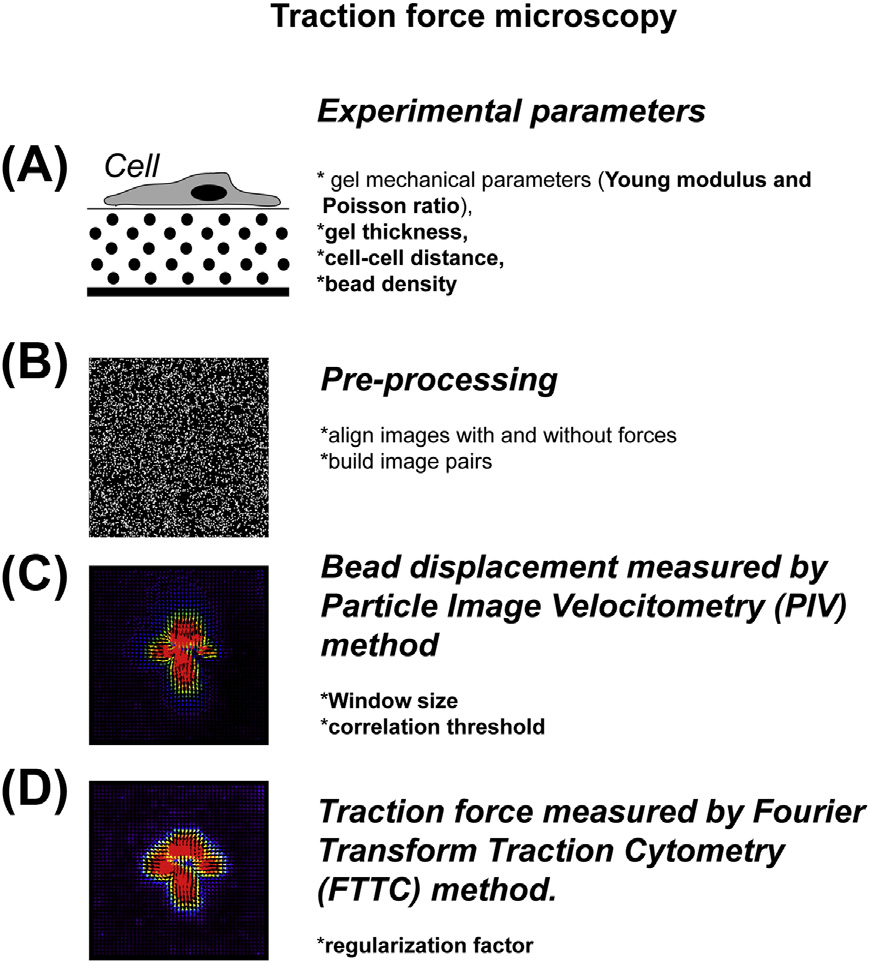
\includegraphics[scale=0.5]{TFM.png}
\caption{\'Etapes du protocole de Traction Force Microscopy, d'après \cite{martiel_measurement_2015}.}
\end{figure}

L'idée de cette technique est d'ensemencer les cellules sur un substrat déformable, en général un gel de polyacrylamide. 
Des billes fluorescentes d'un diamètre de l'ordre de la centaine de nanomètres à l'intérieur du gel servent de traceurs. 
Lorsque la cellule exerce des forces sur le substrat, le gel est déformé et les billes sont déplacées. 
Les cellules sont alors décollées, ce qui permet au gel de reprendre sa forme au repos et donc d'avoir la position initiale des billes. 
La connaissance des propriétés mécaniques du gel permettent de remonter du champ de déformation dans le gel sous et autour de la cellule au champ de contraintes exercées par la cellule, par exemple pour observer les mécanismes qu'elle utilise pour se mouvoir \parencite{delanoe-ayari_4d_2010}.

Cette technique peut s'utiliser à l'échelle d'une cellule unique lorsque les cellules sont suffisamment éloignées les unes des autres pour que les champs de déformation qu'elles causent ne se superposent pas. 
Elle peut également être utilisée à l'échelle d'un tissu lorsqu'on ne cherche pas à démêler la contribution individuelle de chaque cellule mais seulement celle du tissu tout entier. 

\cite{martiel_measurement_2015} proposent une description complète de cette technique. 

\subsubsection{Substrats texturés}

On peut remonter plus facilement aux forces générées par la cellule en les ensemençant sur un champ de piliers en PDMS de 2 \micro m de diamètre et d'une dizaine de \micro m de haut. 
En effet, la raideur des piliers peut être calibrée à l'avance, et retrouver la force exercée sur le pilier à partir de sa déflexion est un problème plus simple à résoudre que celui du champ de déformation de la TFM (\cite{du_roure_force_2005}). 

Cette technique peut être combinée à d'autres : le champ de micro-piliers en PDMS peut ensuite être étiré pour observer comment la génération de forces est modifiée par la déformation extérieure, les micro-piliers peuvent être recouverts de motifs de protéines d'adhésion de formes et de tailles contrôlées, ou des particules magnétiques peuvent être incorporées à l'intérieur des piliers pour contrôler leur déflexion avec un champ magnétique \parencite{gupta_micropillar_2015}. 

\subsubsection{Contrôle de la forme}

Le forme des cellules peut être hautement variable d'un type cellulaire à l'autres, mais également à l'intérieur d'un même type cellulaire. 
Ainsi, dans une population de C2C12, certaines cellules ont une forme allongée, d'autres plutôt triangulaire, certaines sont rondes, et leur taille peut également varier d'un facteur 10. Au contraire, lorsque les mêmes cellules sont différenciées en myotybes, elles ont toutes une forme très allongée. 

Ces différences de taille et de formes sont autant de paramètres géométriques hors de contrôle de celui qui veut mesurer les paramètres physiques des cellules et en déduire des principes généraux. 

C'est pour réduire cette variabilité qu'ont été développées les techniques de micro-patrons adhésifs. 
Le principe est de créer sur le substrat des zones recouvertes de protéines adhésives de forme et de taille contrôlées (\cite{thery_adhesive_2009}).
Une cellule ne pourra adhérer que sur ces zones, le reste de la surface étant rendue non-adhésive. 

Cette technique a été utilisée dans différents contextes pour étudier la manière dont MRTF-A régule la transition EMT. 
Dans le premier cas, les cellules ont été ensemencées individuellement sur des disques d'aires différentes (\cite{connelly_actin_2010}). Sur les disques de taille trop faible pour que la cellule puisse s'étaler, MRTF-A était accumulée dans le noyau, contribuant au changement de type cellulaire. 
Dans le second cas, les cellules étaient ensemencées sur des motifs carrés d'une centaine de microns de côté (\cite{gomez_tissue_2010}). Les cellules sur les bords subissaient alors plus de contraintes et de tension que les cellules du centre du motif, et MRTF-A était nucléaire dans les cellules des bords du carré, et cytoplasmique dans les cellules à l'intérieur.

Dans les deux cas, la forme et l'aire proposées à la cellule déterminent suffisamment l'état du cytosquelette pour induire la translocation de MRTF-A.  
\begin{figure}
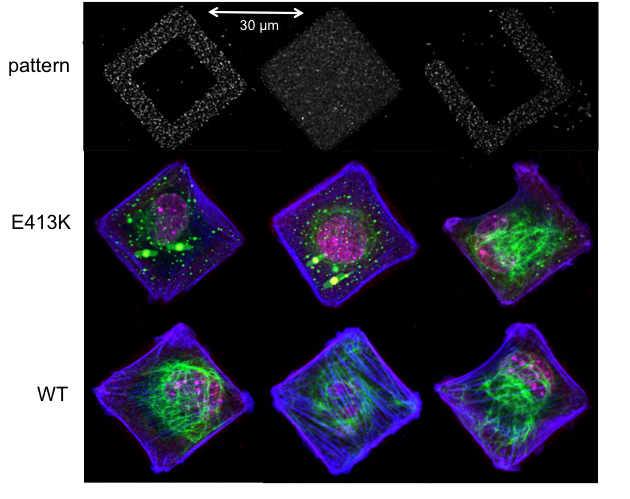
\includegraphics[scale=0.7]{Patterns_elisabeth.png}
\caption{Images de C2C12 sauvages et possédant une version mutante de la desmine (E413K) sur des micro-patrons adhésifs. Les filaments d'actine sont marqués à la phalloïdine Alexa 647 (en bleu), les filaments de desmine-GFP sont en vert, les noyaux sont marqués au DAPI (en magenta) et le motif en fibronectine Cy3.5 (en rouge), d'après \cite{charrier_implication_2014}. }
\end{figure}
\subsubsection{Méthodes également utilisées en rhéologie active}

Une partie des méthodes de rhéologie active peuvent également être utilisées pour mesurer des forces dans des montages un peu différents de celui utilisé pour la rhéologie. 

C'est le cas par exemple pour les expériences sur les forces d'adhésions entre deux cellules, qui peuvent être faites avec deux micropipettes (une cellule attachée à chacune) \parencite{biro_dual_2015}, ou avec une cellule attachée à la lamelle souple d'un AFM pour sonder une autre cellule sur le substrat. 

Même s'il est présenté dans les techniques de rhéologie active, le rhéomètre à cellule unique peut être également utilisé pour mesurer les forces générées par une cellule. 
La cellule est alors attrapée entre les deux plaques et laissée libre de s'étaler. La force qu'elle exerce sur les plaques est déduite de la déflexion de la lamelle souple, ce qui permet de mesurer la force totale que la cellule peut développer (\cite{mitrossilis_single-cell_2009}). 

\subsection{Appliquer des forces pour observer la réponse biologique}

La mécanotransduction s'intéresse particulièrement à la réponse biologique des cellules soumises à des contraintes mécaniques. 
Il est alors important de pouvoir leur appliquer de manière contrôlée des contraintes pour observer les changements biologiques que cela provoque. 

Une grande partie des techniques de rhéologie active présentées précédemment peuvent être utilisées pour appliquer des forces contrôlées aux cellules, car la majorité d'entre elles sont compatibles avec des observations sur leur état biologique.

Par exemple, \cite{zhao_force_2007} ont utilisé des billes magnétiques pour appliquer une contrainte verticale constante à des fibroblastes cardiaques de rat. Ils ont observé une activation de la voie RhoA/ROCK en réponse à la force, qui aboutit à la désactivation de la cofiline. Cela stabilise alors les filaments d'actine, MRTF-A est alors accumulée dans le noyau et le promoteur de l'$\alpha$-actine  du muscle lisse est activé. 

Les cellules peuvent également être cultivées sur des substrats déformables, la plupart du temps des gels de polyacrylamide ou de PDMS, recouverts de protéines d'adhésion, qui seront soumis à des déformations constantes ou cycliques. Des étirements cycliques ont ainsi été appliqués par \cite{kuwahara_myocardin-related_2010} sur des myocytes cardiaques de rat et induisent une accumulation nucléaire de MRTF-A. 
Un dispositif permettant ce type de stimulation constante est décrit dans le chapitre de cette thèse concernant les méthodes expérimentales.  


Le développement de la microfluidique ouvre un nouveau champ de recherches en mécanique cellulaire, en permettant d'appliquer non pas des forces ou des couples mais directement des contraintes, tout en contrôlant de manière fine et rapide l'exposition aux facteurs biochimiques. 
Par exemple, l'observation de cellules en train de passer à travers de pores de quelques micromètres de diamètre apporte de nouvelles informations sur la manière dont les cellules se déplacent \textit{in vivo} dans une matrice extra-cellulaire en 3D \parencite{aubry_computational_2015}. 

Une grande partie des observations de migration et de motilité cellulaires sont faites, pour des raisons pratiques évidentes, sur des substrats plats et bien plus rigides que les tissus biologiques. Au fur et à mesure qu'apparaît l'importance de l'environnement mécanique pour les cellules, il devient de plus en plus essentiel de développer des environnements de culture plus proches de la physiologie. Les méthodes de culture et de visualisation de cellule en 3D dans des matrices de bio-polymères de rigidité contrôlée sont en plein essor, malgré les obstacles techniques \parencite{fischer_stiffness-controlled_2012}. 

%\end{document}



%\documentclass                                                                                                                                                                                                                                                                                                                                       {report}
%\usepackage[T1]{fontenc}
%\usepackage[utf8]{inputenc}
%\usepackage[francais]{babel}
%\usepackage{amsmath}
%\usepackage{graphicx}
%\graphicspath{{Figures/}}
%\usepackage[backend=biber,style=authoryear,bibencoding=utf8]{biblatex}
%\usepackage[colorlinks,linkcolor=blue]{hyperref}
%\newcommand{\micro}{$\mathrm{\mu}$}
%\addbibresource{biblio2.bib}
%
%\begin{document}

\chapter{Méthodes et dispositifs expérimentaux}
\begin{figure}

\includegraphics[scale=0.7]{Chapitre6.png}

\end{figure}
\newpage

\section{Culture cellulaire}
	\subsection{Type cellulaire : les C2C12}
	
	\begin{figure}
	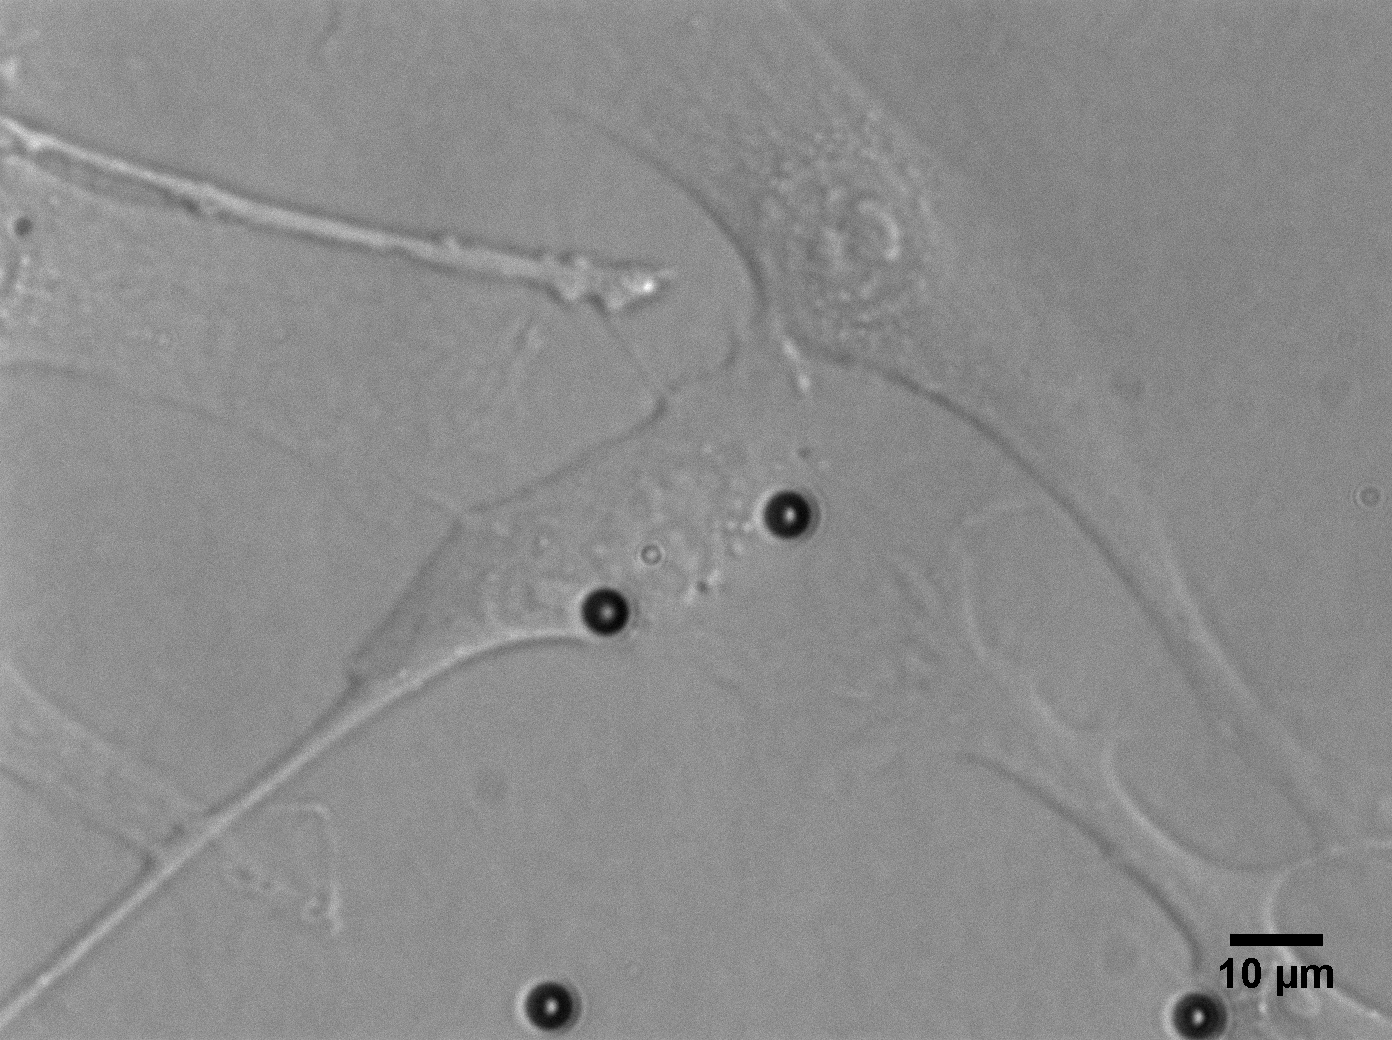
\includegraphics[scale=0.15]{c68-avt.png}
	\caption{C2C12 en culture sur du verre, avec des billes de 4,5 microns de diamètre, observées au microscope à immersion 100X.}
	\end{figure}
	
	Nous avons utilisé comme modèle une lignée immortalisée de myoblastes murins de l'ATCC, les C2C12. Elles présentent l'avantage d'être la lignée immortalisée la plus proche des cellules qui sont utilisées par nos partenaires de l'Institut Cochin dans leurs expérimentations animales sur les souris. 
	
	Ce sont des cellules adhérentes qui conservent leur capacité à se différencier en myotubes lorsqu'elles atteignent la confluence et sont placées dans un milieu pauvre en sérum. C'est pourquoi il est essentiel de les maintenir en permanence en-dessous de la confluence. 
	
	Elles adoptent des formes variées (allongées, triangulaires, en disque) et se déplacent sur leur surface de culture en étendant des lamellipodes. 
	
	Les C2C12 sont cultivées dans un milieu de culture composé de DMEM (Dulbecco's Modified Eagle Medium) à 4,5g/L de L-Glucose supplémenté de 10\% de Sérum de Veau F\oe tal (SVF) et de 1\% d'antibiotiques (Pénicilline et Streptomycine) dans un incubateur à 37\degres   C et 5\% de CO$_2$. 
	
	
	Lorsqu'elles sont proches de la confluence, il faut rincer deux fois les cellules avec du PBS (Phosphate Buffered Saline) et les laisser incuber 5 minutes à 37\degres   C dans un mélange Trypsine/EDTA. La trypsine est une enzyme qui va casser les adhésions cellulaires, tandis que l'EDTA joue le rôle de chélateur des ions calcium qui sont indispensables pour créer des adhésions. Une fois les cellules décollées, elles sont diluées dans du milieu de culture qui inactive la trypsine et ensemencées à nouveau sur des boîtes de culture. Cette opération s'appelle le passage. 
	 
	\subsubsection{Culture sur PDMS ou sur verre des C2C12 \label{Coating}}

	Pour réaliser les différentes expériences de rhéologie cellulaire, les cellules doivent être cultivées sur d'autres substrats que dans les boîtes de cultures : sur des lamelles de verre carrées (22mmm x 22mm x 100 \micro m) dans le cas des pinces magnétiques et sur des disques de PDMS (30mm de diamètre et 0.3 mm d'épaisseur) dans le cas de l'étirement. 
	
	Les disques de PDMS doivent préalablement être passées dans un four à plasma pendant 2 minutes afin de rendre leur surface hydrophile. Cette opération stérilise également les disques. Les lamelles de verre doivent être stérilisées 30 minutes à l'aide d'un rayonnement UV. 
	
	Les lamelles comme les disques sont placés dans les puits d'une plaque 6 puits, et mis à incuber 30 minutes à 37\degres   C dans 1ml de milieu complet et 5\micro g de fibronectine qui va s'adsorber sur la surface. 
	
	Après rinçage, \nombre{110 000} cellules sont ensemencées sur chaque lamelle dans du milieu complet. 
	
	\subsection{Les myoblastes primaires}
	
	Durant la fin de ma thèse, Tiana Jacquemart, en stage de M1 dans notre équipe, a réalisé des expériences sur des myoblastes primaires de souris. Ces myoblastes avaient été infectés avec un lentivirus par Alessandra Pincini, en post-doc à l'Institut Cochin et dans notre laboratoire, pour leur faire exprimer MRTF-A GFP (voir les précisions dans les sous-sections suivantes). 
	
	Les myoblastes primaires sont plus fragiles, et doivent être cultivées dans des conditions différentes des C2C12. Elles sont cultivées dans un un milieu de prolifération composé de 500 \micro de DMEM F12 sans Glutamax avec HEPES, 100 \micro l de Serum de Veau F\oe tal (SVF), 5 \micro l d'un mélange d'antibiotiques et d'anti-mitotiques, 8 \micro l de Glutamine et 10 \micro l d'Ultroser. Ce milieu est donc beaucoup plus riche en facteurs de croissance que le milieu de culture des C2C12. 
	
	Elles sont cultivées dans des boîtes de Petri de diamètre 10 ou 15cm recouvertes de 5 à 10 ml de gélatine 0,02\% (préparée avec de l'eau stérile).
	
	Lorsqu'elles sont proches de la confluence, il faut rincer les cellules avec du PBS (Phosphate Buffered Saline) et les laisser incuber 1 minute à 37\degres   C dans un mélange Trypsine/EDTA. Une fois les cellules décollées, elles sont suspendues dans un tube avec 10 ml de milieu de culture sans Ultroser, mélangées puis comptées. La quantité désirée de cellules (en général une centaine de milliers) est alors centrifugée 7  minutes à 1700 tours/minute. Le surnageant est jeté, et le culot suspendu dans le milieu de culture , cisaillé et ensemencé dans une nouvelle boîte de Petri. 
	
	\subsubsection{Culture sur Flexcell}
	
	Les myoblastes primaires adhèrent mal sur les lamelles de PDMS recouvertes de fibronectine que nous utilisons pour les C2C12. Ils sont ensemencés sur des lamelles de Flexcell (Flexcell International Corporation) qui sont vendues déjà recouvertes de collagène I. Après un passage comme décrit dans le paragraphe précédent, on ensemence environ 100 000 cellules sur une lamelle de Flexcell. 
	Lorsqu'elles sont dans leur milieu de prolifération, les cellules primaires sont très motiles, et donc peu sensibles à l'étirement. C'est pourquoi, pour se rapprocher des conditions des C2C12, au moment où les myoblastes sont ensemencés sur les Flexcells, leur milieu est remplacé par le milieu des C2C12 (DMEM sans rouge phénol à 4,5g/L de L-Glucose supplémenté de 10\% de SVF et de 1\% d'antibiotiques). 
	
	\subsection{Visualiser une protéine dans la cellule : anticorps, marqueurs et protéines fluorescentes}
	
	Trois techniques ont été utilisée pendant cette thèse pour visualiser nos deux protéines d'intérêt, l'actine et MRTF, dans les cellules. 
	
	La première et la plus ancienne fait appel à des anticorps spécifiquement dirigés contre la protéine cible. Une fois que les anticorps se sont fixés sur leurs cibles, un anticorps secondaire couplé à un fluorophore vient détecter et se fixer sur le premier anticorps. 
	
	La seconde fait appel à des molécules spécifiquement dirigées contre notre protéine d'intérêt et couplées à un fluorophore. C'est le cas par exemple de la phalloïdine, drogue issue de l'Amanite Phalloïde qui a la propriété de se fixer aux filaments d'actine.	
	
	La dernière technique fait appel à la Green Fluorescent Protein (GFP), protéine découverte dans les années soixante chez une méduse, et utilisée à partir des années 90 pour marquer des protéines. En fusionnant la séquence génétique de la GFP avec la séquence de la protéine à observer, on obtient un nouveau gène codant pour une version fluorescente de la protéine d'intérêt. Après introduction du gène dans les cellules, celles-ci expriment alors la version fluorescente de la protéine. Cette utilisation de la GFP a révolutionné la biologie cellulaire et a été l'objet du prix Nobel de Chimie en 2008. Aujourd'hui, il existe de nombreuses variantes de cette technique, que ce soit au niveau des bandes d'émission et d'absorption du fluorophore (il en existe de toutes les couleurs du spectre visible) ou au niveau de la manière dont le gène de la nouvelle protéine est intégrée dans les cellules (transfection, électroporation, infection par des virus  \dots).
	
	Cette dernière technique permet d'observer la protéine fluorescente en direct pendant la vie de la cellule, alors que la première technique ne peut être utilisée que sur des cellules fixées. La seconde technique peut parfois être utilisée sur des cellules vivantes lorsque la drogue utilisée n'est pas trop toxique. 
	
	\subsubsection{Visualiser le cytosquelette d'actine dans le cadre des expériences sur MRFT-A}
	
L'observation en direct du cytosquelette d'actine est particulièrement intéressant car le système est très dynamique, ce que ne peuvent pas capturer les expériences sur cellules fixées.
Cependant, cela signifie qu'il faut trouver un moyen d'observer l'état du cytosquelette en le perturbant le moins possible. 

Durant cette thèse, j'ai testé quatre moyens d'observer l'actine ou les filaments d'actine dans les cellules vivantes. Tous se sont finalement révélés perturber dans une certaine mesure l'état du cytosquelette. 

La première méthode d'observation de l'actine dans les cellules vivantes est de leur faire exprimer, en plus de l'actine endogène, un autre gène codant pour une actine fluorescente, en l'occurence ici une actine dotée d'un fluorophore mCherry. 
Elle a l'avantage de marquer toute l'actine, et pas seulement les filaments comme les méthodes qui seront présentées après. 
Mais elle a le désavantage de faire sur-exprimer l'actine à la cellule, de manière variable d'une cellule transfectée à l'autre. 
Or MRTF-A est une sonde extrêmement sensible de la quantité de G-actine dans la cellule.  Sur-exprimer l'actine augmente la quantité totale d'actine G, et a un effet très visible sur MRTF-A, comme il sera présenté au chapitre 8. 

Les trois autres méthodes sont des détecteurs qui marquent uniquement les filaments d'actine, avec l'avantage de voir plus nettement la structure du cytosquelette. Il est à noter qu'actuellement il n'existe aucune sonde commercialisée pour observer l'actine monomérique \textit{in vivo}, même si une sonde a été développée récemment à partir des groupes RPEL de MRTF-A \parencite{belin_visualization_2013}. 

La LifeAct est une petite protéine de seulement 17 acides aminés qui se lie aux filaments d'actine \parencite{riedl_lifeact:_2008}. Adjointe à un fragment de protéine fluorescente, comme la GFP ou mCherry, elle permet d'observer les filaments dans les cellules vivantes.  Son ADN doit être transfecté dans la cellule pour y être exprimé avant observation. Elle a été présentée comme un moyen s'observer les filaments sans les perturber, et sans affecter leur polymérisation et leur dépolymérisation. Cependant, et comme ce sera présenté au chapitre 8, la LifeAct n'est pas complètement sans influence sur le cytosquelette d'actine. On constate une tendance à stabiliser les filaments d'actine qui est visible par l'observation de MRTF-A. 

La F-tractin \parencite{johnson_neuronal_2009} est un fragment de protéine constitué des 66 premiers acides aminés de l'inositol trisphosphate 3-kinase A, qui se lie aux filaments d'actine. Comme la LifeAct, sa séquence codante doit être exprimée par la cellule avant observation. Comme la Life, j'ai également observé une tendance de la F-tractin à stabiliser suffisamment les filaments d'actine pour affecter la localisation de MRTF-A. 

Enfin, la SiRactine est une des dernières sondes développées pour marquer les filaments d'actine \textit{in vivo} \parencite{lukinavicius_fluorogenic_2014}. Il s'agit d'un fluorophore Silicone-Rhodamine conjugué à un fragment de la japlakinolide, drogue connue pour se lier aux filaments d'actine et les stabiliser. Cette construction a pour particularité, par un mécanisme d'activation, d'être 100 fois plus fluorescentes lorsqu'elle est liée aux filaments d'actine que dans l'état non-lié, ce qui minimise le bruit de fond. La qualité de la fluorescence devait permettre d'utiliser la SiR-actine dans des quantité suffisamment faibles pour que l'influence stabilisatrice du japlakinolide sur les filaments d'actine soit invisible. Un effet sur les expériences avec MRTF-A est néanmoins visible. 

MRTF-A est une sonde extrêmement sensible de l'état du cytosquelette de la cellule, et toutes les méthodes que nous avons utilisées pour visualiser le cytosquelette \textit{in vivo} ont montré des effets sur sa localisation dans une population de cellules. 
	
	
	\subsection{Transfections}
	Afin de visualiser les protéines qui nous intéressent, on ajoute aux cellules de l'ADN non chromosomique d'origine bactérienne appelés plasmides qui codent pour une version fluorescente de nos protéines d'intérêt. Ces plasmides sont intégrées aux cellules grâce à des agents spécifiques comme la nanofectine et la lipofectamine lors de la transfection. 
	
	\begin{figure}
	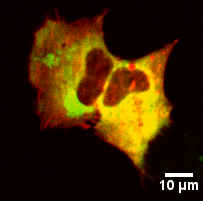
\includegraphics[scale=0.75]{C2C12_RGB-1.png}
	\caption{C2C12 transfectées avec un plasmide MRTF-A GFP (en vert) et un plasmide Actine Mcherry (en rouge)}
	\end{figure}
	
	Les cellules transfectées expriment donc deux versions de la protéine : la version endogène qui se trouve dans leur propre génome, et la version fluorescente du plasmide. La protéine que l'on observe est par conséquent toujours surexprimée par rapport à la situation normale, d'un facteur qui peut être variable d'une cellule à l'autre, selon la quantité de plasmide qui a été intégrée par la cellule : certaines cellules n'ont incorporé aucun plasmide et ne sont donc pas fluorescentes, d'autres en ont incorporé une grande quantité et sont très fluorescentes. 
	
	La transfection est d'autant plus efficace que les cellules sont proches de la confluence. Cependant, on ne peut pas laisser les C2C12 atteindre la confluence, l'efficacité de transfection est donc toujours limitée. La transfection peut se faire avant ou après l'ensemencement des cellules sur leur substrat (verre ou PDMS selon l'expérience). Lorsque la transfection a lieu avant l'ensemencement, elle est faite directement dans la boîte de culture, alors que lorsqu'elle est faite après, elle a lieu dans les puits. 
	
	 Dans les protocoles suivants, les proportions sont données pour un puits d'une plaque 6 puits. Une petite boîte de culture (T-25) représente une surface de 2,5 fois celle d'un puits, les quantités utilisées lors de la transfection d'une boîte sont donc multipliées d'autant.
	
	\subsubsection{Protocole de transfection à la nanofectine}
	
	Trois protocoles sont décrits simultanément ici : le protocole pour une transfection simple de MRTF-A GFP , puis pour une transfection double MRTF-A GFP/Actine Mcherry (option 1) ou MRTF-A GFP/LifeAct RFP (option 2). Sauf indication contraire, toutes les étapes et ingrédients optionnels sont en plus des ingrédients pour la transfection simple.
	
\paragraph{Ingrédients :}
\begin{quote}

	\begin{itemize}
	\item Des C2C12 ensemencées dans un puits d'une plaque 6 puits
	\item 1 \micro g de nanofectine (PAA Nanofectin Kit)
	\item 1 \micro g d'ADN de MRTF-A GFP
	\item (option 1 : Actine Mcherry) 1 \micro g d'ADN d'Actine Mcherry
	\item (option 1 : Actine Mcherry) 1 \micro g de nanofectine
	\item (option 2 : LifeAct RFP) 0,75 \micro g d'ADN de LifeAct RFP
	\item (option 2 : LifeAct RFP) 0,75 \micro g de nanofectine
	\item 2*50 \micro l de NaCl 150mM
	\item (option 1 ou 2) 2*50 \micro l de NaCl 150mM
	\item 0,9ml de milieu complet (transfection simple uniquement)
	\item (option 1 ou 2) 0,8 ml de milieu complet
	\end{itemize}
\end{quote}

\paragraph{Protocole : }
\begin{quote}
\begin{enumerate}
	\item Diluer dans un eppendorf 1 \micro g de MRTF-A GFP dans 50 \micro l de solution de NaCl 150mM. 
	\item Diluer de même 1 \micro g de nanofectine
	\item (option 1 ou 2 ) Répéter ces deux étapes avec l'Actine mCherry ou la LifeAct RFP
	\item Transvaser le contenu de l'eppendorf de nanofectine dans l'eppendorf d'ADN (le sens est important)
	\item (option 1 ou 2 ) Répéter l'opération pour les deux autres tubes
	\item Laisser incuber 30 minutes à 37~\degres C 
	\item Transvaser le ou les mélange(s) nanofectine + ADN dans du milieu complet de façon à obtenir 1  ml de solution
	\item Rincer les cellules
	\item Ajouter le mélange nanofectine + ADN + milieu complet sur les cellules
	\item Laisser incuber à 37 \degres C pendant au moins 6 heures
	\item Enlever le mélange, rincez et remplacez avec du milieu complet
	\item Laisser les cellules exprimer le plasmide entre 12 et 24h après rinçage
\end{enumerate}
\end{quote}

\subsubsection{Protocole de transfection à la lipofectamine}

Suite au rachat de notre fournisseur, la nanofectine n'est plus commercialisée. Les expériences suivantes ont donc été réalisées avec de la lipofectamine (Lipofectamine 3000 Transfection Kit, Invitrogen). Deux protocoles sont décrits ici en même temps : MRTF-A GFP avec et sans F-tractine RFP. 

\paragraph{Ingrédients :}
\begin{quote}

	\begin{itemize}
	\item Des C2C12 ensemencées dans un puits d'une plaque 6 puits
	\item 6 \micro l de lipofectamine 3000 
	\item 1 \micro g d'ADN de MRTF-A GFP
	\item 2 \micro l de P3000 Reagent
	\item (option 1 : F-tractine) 1 \micro g d'ADN de F-tractine RFP
	\item (option 1 : F-tractine) 6 \micro l de lipofectamine 3000
	\item (option 1 : F-tractine) 2 \micro l de P3000 Reagent
	\item 2*125 \micro l d'OptiMEM (Opti-MEM I Reduced Serum Medium, Gibco)
	\item 0,75ml de milieu complet (transfection simple uniquement)
	\end{itemize}
\end{quote}
\paragraph{Protocole : }
\begin{quote}
\begin{enumerate}
	\item Dans l'eppendorf \no 1, mélanger 6 \micro l de lipofectamine 3000 et 125 \micro d'OptiMEM. 
	\item (option 1) Répétez cette étape dans l'eppendorf \no 1bis. 
	\item Dans l'eppendorf \no 2 mélanger 1\micro g de plasmide MRTF-A GFP, 2 \micro l de P3000 Reagent et 125 \micro l d'OptiMEM.
	\item (option 1) Dans l'eppendorf \no 2bis mélanger 1\micro g de plasmide F-tractine, 2 \micro l de P3000 Reagent et 125 \micro l d'OptiMEM.
	\item Transvaser le contenu de l'eppendorf \no 2 dans l'eppendorf \no 1. 
	\item (option 1) Transvaser le contenu de l'eppendorf \no bis2 dans l'eppendorf \no 1bis. 
	\item Laisser incuber 5 minutes à 37\degres C. 
	\item (MRTF-A GFP seule) Mélanger à 1.75 \micro l de DMEM sans rouge phénol.
	\item (option 1) Mélanger les eppendorfs \no 2 et \no 2bis à 1.5 \micro l de DMEM ans rouge phénol
	\item Rincer les C2C12 et leur ajouter les 2ml de solution. 
	\item Laisser incuber une nuit à 37 \degres C.
	\item Ne pas rincer avant les expériences.
\end{enumerate}
\end{quote}

	\subsection{Marquage DAPI sur cellules vivantes}
	
	Le  4',6'-diamidino-2-phénylindole (DAPI) est une molécule fluorescente qui peut se fixer entre les bases A et T de l'ADN. Elle peut entrer dans les cellules vivantes et permet ainsi de marquer l'ADN du noyau. Sa localisation dans l'ADN perturbe la réplication de l'ADN nécessaire à la division cellulaire, c'est pourquoi le DAPI est ajouté à la dernière minute avant les expériences sur cellules vivantes. 
	
	Trente minutes avant l'observation, du DAPI est ajouté au milieu de culture en proportion 1/1000 ou 1/500 (selon l'efficacité du lot de DAPI pour entrer dans les cellules). Il est si possible rincé avant l'observation pour améliorer le contraste. 
	
	\subsection{Marquage SiRactine sur cellules vivantes}

	La SiRactine est un marqueur des filaments d'actine qui peut être ajouté aux cellules vivantes avant l'observation. Elle a un pic d'absorption à 652 nm et un pic de fluorescence à 674 nm, ce qui la rend compatible avec les plasmides fluorescents dans le vert (comme la GFP) et dans le rouge (comme la mCherry ou la RFP). 
	
	La SiRactine pouvant avoir un effet de stabilisation des filaments d'actine, lorsqu'on l'utilise sur des cellules vivantes, il faut trouver la concentration minimale nécessaire à l'observation. Plus la concentration utilisée est faible, plus il faudra la mettre longtemps à l'avance sur les cellules. 
	
	La quantité de SiRactine désirée est ajoutée la veille ou 3 heures avant l'observation (selon la concentration) sur les cellules, et ne doit pas être rincée. 
	
	Une série de dilutions allant de 50nM à 500nM a été testée préalablement aux expériences, puis trois conditions ont été utilisées : 50 nM incubé toute la nuit, 50nM incubé 3 heures et 2,5nM incubé toute la nuit. 
	
	
	
	\subsection{Fixation}
	La fixation permet de figer les protéines des cellules à un instant donné. Elle est réalisée en ajoutant sur une lamelle recouverte de cellules préalablement rincée au PBS une solution à 4\% de paraformaldéhyde (PFA) pendant 20 minutes à température ambiante. Cette solution est ensuite rincée au PBS. 
	
	Les lamelles fixées ainsi obtenues peuvent être conservées plusieurs mois à 4\degres   C et observées longuement au microscope. 
	\subsection{Marquages sur cellules fixées}
	Les cellules fixées peuvent être marquées par des molécules fluorescentes qui peuvent être perturbatrices ou toxiques pour des cellules vivantes. Ici nous avons réalisé sur cellules fixées des marquages à 4 couleurs : rouge profond pour les filaments d'actine, rouge pour l'actine monomérique, vert pour la MRTF-A et bleu pour l'ADN. 
		\subsubsection{Perméabilisation}
		Afin de faire rentrer les molécules et protéines qui vont nous permettre de marquer les protéines des cellules, il est nécessaire de perméabiliser les cellules. Pour cela, on va ajouter aux cellules fixées une solution contenant 0.5\% de Triton, un tensio-actif qui va permettre de créer des trous dans les membranes plasmiques des cellules fixées. 
		Pour améliorer la spécificité des différents marqueurs on va également saturer les sites de liaison des protéines à l'aide de protéines non spécifiques : Bovine Serum Albumine (BSA) 4\% et Horse Serum (HS) 5\%. 
		
		Les lamelles de cellules fixées sont donc initialement laissées 3h à température ambiante dans la solution de saturation composée de 0.5\% triton, 5\% HS et 4\% BSA. 
		
		\subsubsection{Phalloïdine}
		La phalloïdine est une drogue issue de l'amanite phalloïde qui se lie aux filaments d'actine et les stabilise. Utilisée \emph{in vivo} elle perturbe significativement le cytosquelette jusqu'à se révéler toxique pour les cellules. 
		
		Sur des cellules fixées, la phalloïdine permet de marquer spécifiquement les filaments d'actine. La phalloïdine   utilisée pendant nos marquages a été ajoutée aux cellules fixées la veille de l'observation et laissée toute la nuit à 4\degres C, et rincée avant observation. 
		\subsubsection{DNaseI}
		La DNaseI est une protéine naturellement présente dans le noyau des cellules et qui découpe l'ADN en morceaux de 4 paires de bases. Son action est bloquée lorsqu'elle est liée à un monomère d'actine. En raison de son action sur l'ADN, elle ne peut pas être utilisée sur des cellules vivantes. Sur des cellules fixées, elle est un marqueur spécifique du monomère d'actine. 
		
		Comme la phalloïdine, elle est ajoutée aux cellules fixées la veille de l'observation et laissée toute la nuit à 4\degres   C. 
		\subsubsection{MRTF-A endogène}
		
		Lorsque les cellules sont fixées, on peut observer la MRTF-A endogène grâce à l'immunofluorescence plutôt que de transfecter de la MRTF-A GFP dans les cellules. Cela nous permet de détecter les protéines sauvages exprimées directement par cellule sans surexpression induite par la transfection. 
		
		Le marquage se fait en deux étapes : le marquage par un anticorps spécifique anti-MRTF-A, puis le marquage de l'anti-corps anti-MRTF-A par un autre anti-corps qui est fluorescent. L'anti-corps primaire est placé pendant 30 minutes à température ambiante. La lamelle est ensuite rincée et on y ajoute l'anticorps secondaire à nouveau pendant 30 minutes à température ambiante, puis on rince à nouveau. 
		 
				
		\begin{figure}
		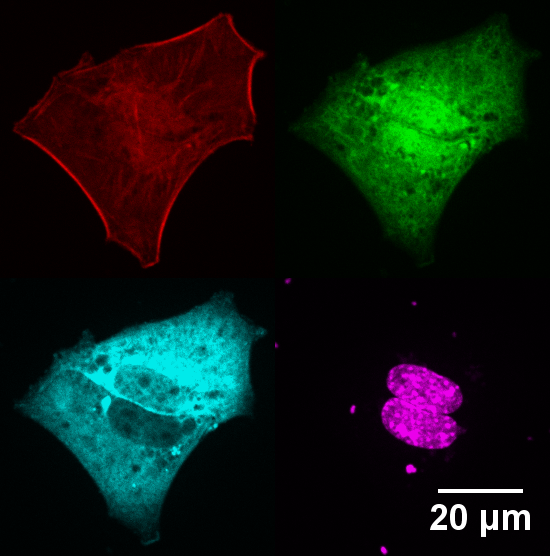
\includegraphics[scale=0.4]{Montage_sc.png}
		\caption{C2C12 transfectées MRTF-A GFP (ici en cyan), fixées et marquées phalloïdine Alexa647 (ici en rouge), DNAseI Alexa547 (ici en vert) et DAPI (ici en magenta)}
		\end{figure}

\subsubsection{Protocole de marquage quadrichrome}
\paragraph{Durée estimée : 3h + 3*30 minutes + une nuit }
 \paragraph{Ingrédients pour une lamelle : }
 \begin{quote}
 
 
 \begin{itemize}
 \item une lamelle de cellules fixées
 \item PBS
 \item 40 \micro g de BSA
 \item 50 \micro l de Horse Serum
 \item 5 \micro l de Triton
 \item 4 \micro l de Phalloïdine Alexa 647 (Life Technologies) 6.6 \micro M dans le méthanol
 \item 1 \micro l de DNase I Alexa 594 (Life Technologies) 161 \micro M dans un mélange 50\% v/v PBS 50\% glycérol
 \item 4 \micro l d'anticorps MRTF-A H140 (Santa Cruz Biotechnology) 200\micro g/ml dans PBS 0.1\% gélatine
 \item 2 \micro l d'anticorps goat anti-rabbit Alexa 488 (Jackson ImmunoResearch) 1.5mg/ml dans de l'eau diluée
 \item 1 \micro l de DAPI
 \end{itemize}
\end{quote}

\paragraph{Protocole pour une lamelle : }
\begin{enumerate}
\item Mélanger 40 \micro g de BSA, 50 \micro l de HS et 5 \micro l de Triton dans 905\micro l de PBS. Le mélange constitue la solution de perméabilisation et de saturation.
\item Enlever le PBS de la lamelle fixée
\item Ajouter la solution de saturation sur la lamelle, et laisser incuber 3h à température ambiante
\item Ajouter 4 \micro l d'anti-MRTF-A H140 à 996 \micro l de PBS
\item Enlever la solution de saturation de la lamelle
\item Ajouter l'anti-MRTF-A diluée et laisser incuber 30 minutes à température ambiante
\item Enlever l'anticorps et rincer deux fois au PBS
\item Ajouter 2 \micro l d'anti-rabbit Alexa 488 dans 998 \micro l de PBS
\item[Attention] à partir de cette étape, pour limiter le photo-blanchiment, il faut éclairer la lamelle le moins possible. Pendant les temps d'incubation, elle doit être protégée par un film opaque. 
\item Ajouter l'anti-rabbit diluée sur la lamelle et laisser incuber 30 minutes à température ambiante
\item Enlever l'anticorps et rincer 2 fois au PBS
\item Ajouter 1 \micro l de DAPI à 999 \micro l de PBS
\item Ajouter le DAPI dilué sur la lamelle et laisser incuber 30 minutes à température ambiante
\item Enlever le DAPI et rincer 2 fois à température ambiante
\item Ajouter 4 \micro l de phalloïdine et 1 \micro l de DNase I à 995 \micro l de PBS
\item Ajouter le mélange phalloïdine et Dnase diluées à la lamelle et laisser incuber toute la nuit.
\item Rincer deux fois avec 1ml de PBS. Les lamelles marquées peuvent être conservées plusieurs semaines à 4\degres C dans l'obscurité, mais la qualité du signal décroît avec le temps, il est donc préférable de les observer le lendemain du marquage.

\end{enumerate}

\section{Pinces magnétiques}

Les pinces magnétiques sont destinées faire de la rhéologie à l'échelle locale sur une cellule unique. Comme les pinces optiques, elles utilisent des billes micrométriques recouvertes de protéines d'adhésion pour s'ancrer à la cellule. 
Une force exercée sur la bille sera alors transmise par les adhésions à la cellule.
 Les contraintes sont donc non seulement ressenties mécaniquement par la cellule, mais aussi biochimiquement au niveau des protéines des complexes d'adhésions. 
La bille, observée au microscope, se déplace en réponse à la force, mais est retenue par la cellule.

Pour étudier la rhéologie cellulaire, on va alors exercer une force connue sur la bille, et mesurer au microscope son déplacement, et donc la déformation de la cellule.
Nous nous sommes placés ici en régime de fluage, plus adapté à la pince magnétique. La bille exerce une contrainte constante sur la cellule $\sigma_0$, qui est reliée à la déformation de la cellule par la relation : 
$$\epsilon (t) = \sigma_0 J(t)$$.

Un modèle nous permet de relier la contrainte subie par la cellule $\sigma_0$ à la force exercée par l'électro-aimant sur la bille $F_0$ et la déformation de la cellule $\epsilon (t)$ au déplacement de la bille $x(t)$. 






Les pinces magnétiques ont été construites pour contourner un certain nombre de limitations que rencontraient les pinces optiques qui existaient déjà au laboratoire, en particulier pour exercer des forces plus grandes pendant des durées plus longues et des découpler l'observation et l'application de force, qui se faisaient par l'intermédiaire de l'objectif dans le cas des pince optiques. Cela s'est fait au prix de la perte de contrôle de la direction de la force : la pince magnétique ne peut que tirer la bille vers la pointe, dans la direction de l'axe de l'électro-aimant. 


	\subsection{Description}
		\subsubsection{Principe}
		Lorsqu'on applique un champ magnétique $$\vec{H} = \frac{\vec{B}}{\mu}$$ sur une bille paramagnétique de volume $V$ et de susceptibilité magnétique $\chi$, cela induit dans la bille un moment magnétique $$\vec{m} = \chi V \vec{H}$$ Si le champ magnétique est de plus inhomogène, la bille subit alors une force :$$\vec{F} = \left( \vec{m}. \vec{\nabla} \right) \vec{B}$$
	
Le principe des pinces magnétiques est donc d'utiliser un électro-aimant, qui va créer un champ et un gradient de champ magnétiques lorsqu'il est alimenté par un courant, pour exercer des forces à distance sur un bille magnétique fixée à la cellule par des protéines d'adhésion. 	 
	 
	 
	 Afin d'exercer cette force, il est nécessaire de construire un électro-aimant répondant à plusieurs contraintes : il doit être capable de créer un fort champ magnétique ainsi qu'un fort gradient de champ magnétique, cependant il ne doit pas chauffer l'échantillon afin de ne pas endommager les cellules vivantes sur lesquelles on manipule, et cela sans système de refroidissement qui risquerait d'introduire un bruit mécanique trop important. L'électro-aimant doit pouvoir être amené le plus près possible de l'échantillon afin d'exercer une force maximale, le plus précisément possible afin de conserver une bonne précision sur la direction et la valeur de la force exercée. On souhaite manipuler avec une chambre expérimentale fermée pour éviter toute contamination des cellules, et pouvoir faire des observations en fluorescence. On souhaite également faire des expériences de longue durée, en imposant des paliers de force pendant plusieurs minutes et répétés pendant plusieurs dizaines de minutes.	
	
		\subsubsection{Billes superparamagnétiques}
		
		\begin{figure}
		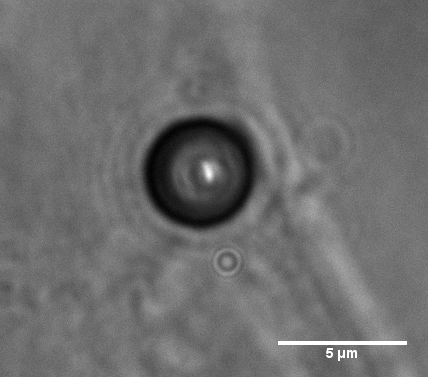
\includegraphics[scale=0.4]{Bille.PNG}
		\caption{Bille Dynabeads M-450 observée en grossissement 150X. }
		\end{figure}
		Les billes utilisées sont des Dynabeads M-450 Epoxy d'Invitrogen Dynal AS, Oslo, Norvège. 
		Ce sont des billes de polystyrène sphériques, de 4,5$\mu$m de diamètre, recouvertes en surface de groupes epoxy afin de permettre l'ajout de ligands en surface, et contenant des nanoparticules d'oxydes de fer qui leur confèrent leurs propriétés superparamagnétiques. 
		Elles sont initialement fournies dans une suspension concentrée ($4.10^8$ billes/ml) dans de l'eau distillée. On les recouvre de fibronectine pour une fixation spécifique aux intégrines.
		Pendant les expériences de pinces magnétiques, la bille magnétique par l'intermédiaire de laquelle on applique une force sur la cellule est observée au microscope à l'aide d'un objectif 100X et filmée pendant toute la durée de l'expérience.  Ces images sont ensuite traitées avec un logiciel d'analyse d'image (ImageJ, National Institue of Health) qui ajuste une ellipse sur l'image des billes. Le logiciel nous donne pour chaque image de chaque expérience le grand axe et le petit axe de l'ellipse ajustée. Une bille est donc mesurée environ \nombre{4 000} fois pendant une expérience.  
		Nous obtenons donc \nombre{385 885} mesures de taille pour 191 billes observées pendant 191 expériences de pinces, avec une taille moyenne de 4.4067 $\pm$ 0.0002 \micro m et un rapport petit axe sur grand axe $e=0.98585 \pm 0.0008$. Les billes apparaissent donc légèrement plus petites qu'annoncé par le fabriquant mais semblent bien sphériques.
		\begin{figure}
		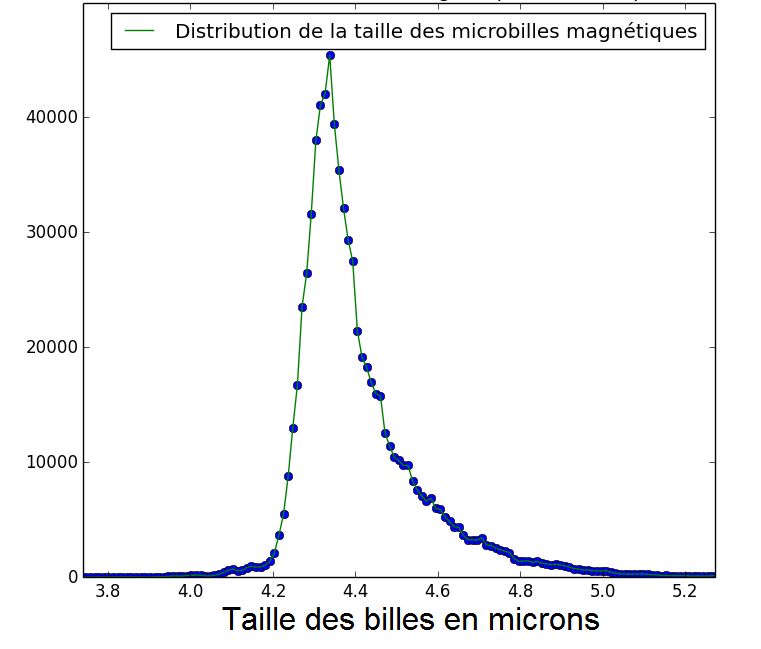
\includegraphics[scale=0.3]{Taille_des_billes.png}
		\caption{Fonction de distribution de taille des billes magnétiques utilisées dans \nombre{191} expériences de pinces. Pour chaque expérience, lorsque la bille est suivie par le logiciel d'analyse d'image, son grand axe et son petit axe sont mesurés pour chaque temps. La fonction est asymétrique car lorsque la bille n'est pas tout à fait au point, son diamètre apparaît plus grand.}
\end{figure}		 
		
		\subsubsection{\'Electroaimant}
		L'électro-aimant est composé d'un c\oe ur entouré d'une bobine de fil de cuivre. Le passage d'un courant électrique dans la bobine crée un champ magnétique dont les lignes de champ sont conduites par le c\oe ur. 
		
		\paragraph{Le c\oe ur} Deux types de c\oe ur ont été testés : un c\oe ur en fer doux (diamètre : \nombre{5.30}mm, longueur : \nombre{52.17}mm) et un c\oe ur en mu-métal, un alliage de grande perméabilité magnétique (diamètre : \nombre{5,10mm} , longueur : \nombre{143,64}mm).
		
		Une extrémité du barreau est taillée en pointe. La forme de pointe permet d'augmenter le gradient de champ magnétique en resserrant les lignes de champ à cet endroit. Il est très important de conserver sa symétrie cylindrique, et d'avoir le rayon de courbure le plus faible possible au bout de la pointe. Les résultats obtenus sont visible en figure $\ref{pointe}$. \'Etant en fer doux, le barreau est très malléable, il faut donc le manipuler avec précautions : le moindre choc aplatit la pointe. 
	 Le barreau a été usiné au tour à l'atelier de mécanique, puis pour la taille d'entretien de la pointe, on monte le barreau sur une perceuse sur pied, ce qui permet de garder la symétrie cylindrique, et on l'approche d'un morceau de papier de verre de grain de plus en plus fin, collée sur une pièce métallique inclinée avec un angle de 30 $\degres$ .
	 
	 \begin{figure}[ht!]%
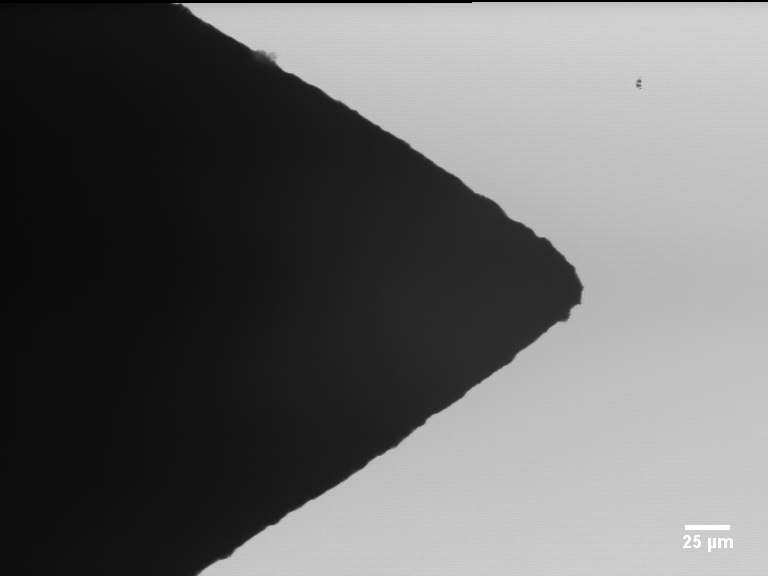
\includegraphics[width=6cm]{pointe1-2011-03-29-20X.png}%
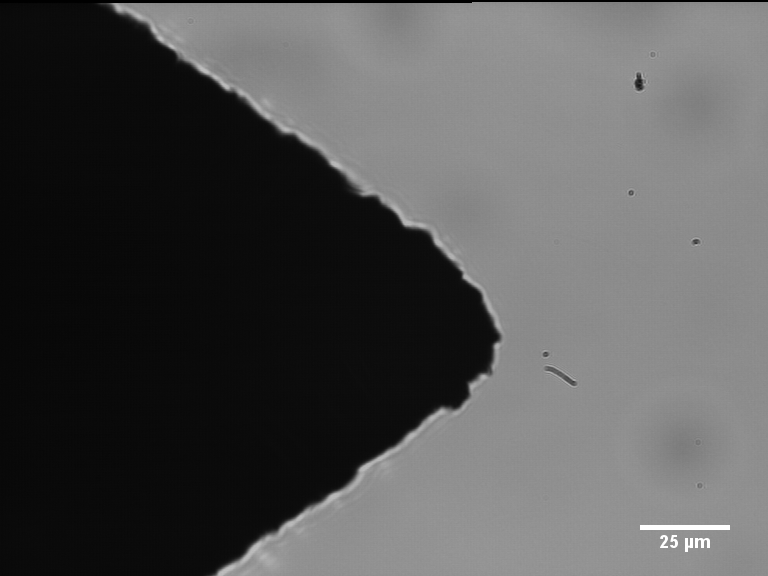
\includegraphics[width=6cm]{pointe1-2011-03-29-40X.png}
\caption{À gauche une image de la pointe en fer doux au grossissement X20. À droite, la même pointe au X40. Le rayon de courbure mesuré est de l'ordre de 2
0$\mu$m.}%
\label{pointe}
\end{figure}
	 
	 L'angle optimal pour maximiser le gradient peut être calculé \parencite{durand_electrostatique_1953}, il vaut environ 55\degres. Ici, on doit aussi prendre en compte le fait que la pointe doit être approchée de biais au-dessus de la lamelle d'échantillon. Il nous faut donc un angle plus faible que l'angle optimal, trop obtus. On a fixé cet angle à 30 $\degres$ , car il est prévu d'approcher la pointe de la lamelle sur laquelle seront les cellules avec un angle de 45 $\degres$, comme représenté sur la figure \ref{montage global} .

\paragraph{La bobine}

	L'optimisation des caractéristiques de l'électro-aimant a été l'objet de mon stage de Master 2. 
	Deux contraintes s'opposent lors de la fabrication : l'augmentation du champ magnétique et l'effet Joule. 
	
	\begin{figure}
	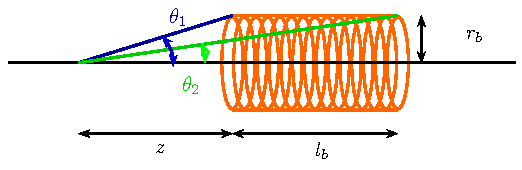
\includegraphics[scale=1]{champB.pdf}
	\end{figure}
	Le champ $\vec{B}$ généré par un solénoïde de longueur finie dans le vide sur son axe à une distance $z$ vaut:
		
		$$ \vec{B} = \frac{\mu_0 n I}{2} \left(\cos \left(\theta_2 -\cos \theta_1 \right)\right) \vec{u_z}$$
		
		Sa valeur dépend du nombre $n$ de spires par mètre, de la longueur de la bobine $l_b$, de son rayon $r_b$ et du courant $I$ qui la traverse. On veut donc maximiser $n$ et $I$ pour augmenter la valeur de $B$. La distance $z$ sera de l'ordre de 700\micro m. 
		
		La puissance dissipée par effet Joule $$P = R I^2$$ dépend de la résistance de la bobine et de $I$, il s'agit de minimiser ces quantités.
		
		La résistance $R$ de la bobine dépend de la section du fil $s$, de sa longueur totale $L$ et de $\gamma$ la conductivité du cuivre :
:
		 $$R = \frac{L}{\gamma s}$$
		
				
		Le nombre de spires par mètre est directement reliée à la section du fil   : $$ n = \frac{1}{2r_f} = \frac{1}{2 \sqrt{\frac{s}{\pi}}} = \sqrt{\frac{\pi}{4s}}$$  Il est facile de voir que lorsque $s$ augmente, $R$ diminue en $s^{-1}$ alors que $n$ ne diminue qu'en $s^{-1/2}$, et donc qu'il faut choisir la section de fil la plus grande disponible.
		En pratique, on ne fait pas qu'une couche de bobinage, mais $n_c$, le nombre de spires par mètres est aussi relié à la longueur totale de fil $L$.
		
		$$R \propto L \approx n_c \frac{\pi r_b l_b}{r_f}$$ où  $l_b$ sa longueur, $r_f$ le rayon du fil. 
		
		$$n = n_c \frac{1}{2r_f}$$
		
		Pour augmenter $n_c$ en augmentant le moins possible $R$, il faut alors minimiser le rapport $\frac{\pi r_b l_b}{r_f}$. On a choisi $r_f$ le plus grand disponible, on prend également $r_b$ le diamètre de la bobine le plus petit possible.
		
		En ce qui concerne la longueur de la bobine, $l_b$, on aimerait la minimiser pour diminuer $R$, cependant, le champ $B$ est maximal pour une bobine de longueur infinie. La longueur optimale correspond en fait à celle du c\oe ur : ajouter de la longueur de bobine au-delà n'augmente que peu le champ, à cause de la faible perméabilité magnétique de l'air.
		
		La bobine finalement utilisée dans nos expériences est composée de 8 couches de fil de cuivre de diamètre 0,5mm bobinées sur un tube d'aluminium de diamètre extérieur égal à 5,38mm sur une longueur de 66,5mm et de diamètre intérieur égal à celui du c\oe ur. Sa résistance est mesurée à 3,3$\Omega$ et son inductance à 1,2mH. 
		
		L'aluminium est un bon support pour la bobine car il est à la fois léger, car il ne faut pas surcharger le micromanipulateur qui portera l'électro-aimant dans le montage final, et qu'il conduit bien la chaleur dégagée par l'effet Joule pour qu'elle soit évacuée vers le c\oe ur. L'aluminium a pu également être taraudé à une extrémité afin d'y attacher une vis de support en laiton qui est tenue par le micromanipulateur, et qui sert également à évacuer une partie de la chaleur de la pointe.                       
		\subsubsection{Montage sous microscope}
		\paragraph{Circuit électrique}
		
		Un générateur de tension basse fréquence, contrôlé par ordinateur par l'intermédiaire d'une carte PCI (Measurement Computing 1208 HS4AO), alimente un amplificateur de courant fabriqué par les ateliers du laboratoire, qui permet de délivrer des courants jusqu'à 2A à la bobine. 
		La bobine ayant à dessein une résistance la plus faible possible pour limiter l'effet Joule, une résistance de 10$\Omega$ est ajoutée au circuit. Un ampèremètre mesure à tout instant l'intensité délivrée à la bobine. 
		
		Le temps de réponse caractéristique du circuit RL est donc de 16ms, ce qui sera négligeable dans toutes les configurations où les pinces seront utilisées. 
		
		 \paragraph{Montage sous le microscope}
		 
		 \begin{figure}
		 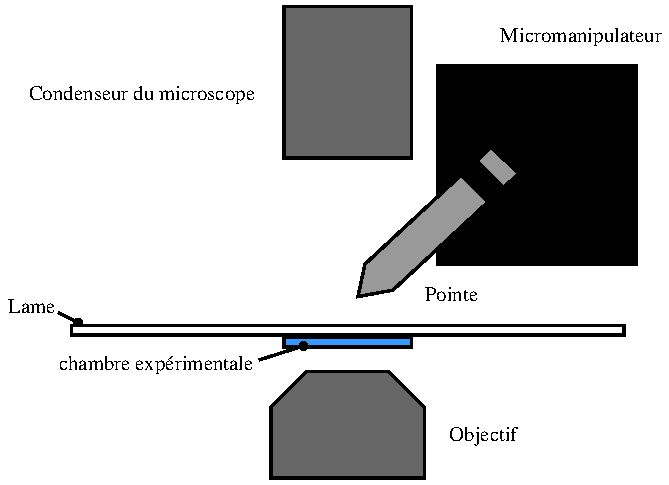
\includegraphics[scale=1]{montageglobal.pdf}
		 \label{montage global}
		 \end{figure}
		 
		 L'électro-aimant que l'on a fabriqué précédemment est monté sur un micromanipulateur (InjectMan NI2, Eppendorf, avec une précision de position de 0.1$\mu$m), incliné à 45 $\degres$ . La force que nous allons exercer sur les billes est parallèle à l'axe de la bobine, nous allons donc appliquer simultanément une force horizontale et une force verticale vers le haut. 
		 
		 Un thermomètre est fixé sur la pointe pour mesurer sa température à tout instant et vérifier qu'il n'y a pas de risque d'endommager les cellules pendant l'expérience. 
		 
		 Les cellules ont préalablement été ensemencées sur une lamelle de verre et incubées avec les microbilles recouvertes de fibronectine. Sur une lame de verre 22mm*64mm*0.15mm, on monte un séparateur (GeneFrame Spacer AB-0577, Thermo Scientific) et la lamelle de verre, le tout formant une chambre expérimentale fermée de 65\micro l emplie de milieu de culture. 		 
		 
		 Le micromanipulateur et la lamelle contenant les cellules sont montés sur un microscope inversé (Leica DMIRB). \`A l'aide du micromanipulateur, on peut approcher la pointe de l'électro-aimant à une distance de 100$\mu$m de la lamelle. On enregistre les images de la bille à l'aide d'une caméra (CoolSnap HQ2) reliée à un ordinateur qui la contrôle par l'intermédiaire de MicroManager. 
		 
		 \begin{figure}
		 \includegraphics[scale=0.5]{modeop1.pdf}
		 \includegraphics[scale=0.5]{modeop2.pdf}
		 \caption{Schéma des deux montages possibles de la lamelle par rapport à l'objectif et à la pince magnétique.}
		 \end{figure}
		 
		 Il existe deux possibilités de montage pour la lamelle : la lamelle sur laquelle sont les cellules peut être placée en haut, du côté de la pointe de l'électro-aimant, ou au contraire en bas, proche de l'objectif du microscope. 
		 
		 Dans le premier cas, la distance entre la pointe de l'électro-aimant et la bobine peut être réduite à 280 \micro m, ce qui permet d'exercer de grandes forces, de l'ordre du nanoNewton. Cependant, la distance entre l'objectif et les cellules est alors d'au moins 400 \micro m, et ne permet pas d'utiliser d'un objectif à immersion, nous restreignant à des grossissements inférieurs à 40X. 

		 Dans le second cas, on peut au contraire utiliser des objectifs à immersion à huile 100X, ce qui nous permet d'avoir une très bonne précision sur la position et sur les déplacements de la bille. Cependant, la distance entre la bille et la pointe est alors de 700 \micro m et il est alors possible d'appliquer au maximum des forces de l'ordre de 160 pN. 
		 
Le choix entre les deux méthodes dépend donc de la précision d'observation dont on a besoin et de la force que l'on souhaite exercer. 

		 
		 
		 		 
		  
		
		
	\subsection{Calibration}
  
 Les caractéristiques magnétiques des billes ne sont pas fournies par le fabriquant, et de plus à des distances inférieures au millimètre, la précision sur les mesures de $\vec{B}$ et $\vec{\nabla}B$ est mauvaise. 
 Il est donc impossible de calculer de manière fiable la force exercée par la pointe sur les billes à un courant et à une distance donnée.
 Pour connaître la force exercée par l'électro-aimant sur les billes en fonction de la distance et du courant, nous avons donc procédé à une calibration.
 
 \subsubsection{Principe}
 
 Les billes de diamètre $d=4.5$\micro m sont placées dans du PDMS liquide de masse volumique $\rho$ proche de celle de l'eau mais de grande viscosité $\eta=0.75$Pa.s. 
 Dans ces conditions, le nombre de Reynolds associé aux billes lorsqu'elles se déplacent à une vitesse $U$ dans le liquide vaut : $$Re = \frac{\rho U d }{\eta}=6*U*10^{-3}$$
 et donc $Re \ll 1$ tant que  $U \ll 167 m.s^{-1}$. 
 On peut donc en conclure que l'inertie est complètement négligeable devant les effets visqueux dans ces conditions. 
 
 Les billes subissent donc deux forces : la force magnétique exercée par la pointe, et les forces de friction visqueuses exercées par le fluide. 
 
 La force de friction visqueuse sur une sphère peut être modélisée par la relation de Stokes : 
 $$ \vec{F}_{vis}=- 3 \pi \eta d \vec{U} =-\vec{F}_{mag}$$
 
 Dans notre dispositif, les billes sont placées dans une chambre expérimentale de 240\micro m de hauteur formée par un séparateur, et l'influence de la lamelle supérieure ou de la lamelle inférieure ne peuvent pas être exclue. On note $h$ la distance à la lamelle la plus proche. 
 De plus, la viscosité $\eta$ du fluide est très sensible aux variations de température, or l'électro-aimant chauffe pendant l'application de la force à cause de l'effet Joule dans la bobine. 
 Comme la mesure est effectuée à une distance de 0,5 à 1mm de la pointe, celle-ci chauffe le fluide localement. 
 On a mesuré la dépendance de la viscosité du fluide en fonction de la température $\dfrac{\eta}{T}=0.0178 Pa.s/\deg C$ autour de 24\degres C. 
 
 Le modèle de Stokes est donc corrigé ainsi : 
 
 \begin{equation}
 {F}_{mag}= 3 \pi \left(\eta_{24^{o}C}-\dfrac{\eta}{T}\left(\frac{T_{fin}-T_{init}}{2} - 24\right) \right) *\left( \frac{d_{max}+d_{min}}{2} \right) * \left( 1+\frac{d}{h} \right)*\vec{U}
 \label{Stokes_corr}
 \end{equation}
 
 \subsubsection{Montage et protocole}
 
 \begin{figure}
 \includegraphics[scale=0.4]{Calibration_pinces.png}
 \label{calibration_pinces}
 \end{figure}
 

 
 L'électro-aimant est monté sur le micromanipulateur à l'horizontale.  
 On suspend 1 \micro l de suspension mère de billes dans 499 \micro l de PDMS, et on passe cette suspension 45 minutes dans une cuve à ultra-sons en cisaillant toutes les 5 minutes.
 La suspension est placée dans une chambre expérimentale formée par une lamelle 22mm*64mm*0.15mm, une lamelle 22mm*22mm*0.1mm et un séparateur de 240 \micro m d'épaisseur. La chambre est ouverte du côté où l'on va approcher la pointe. 
 
 La chambre expérimentale est placée sous un microscope droit Reichert doté d'un objectif 5X et d'un 20X et d'une caméra reliée à un ordinateur. Le protocole d'étalonnage est alors le suivant : 
 
 \begin{quote}
 \begin{enumerate}
 \item Placer le plan focal au centre de la chambre expérimentale selon l'axe vertical.
 \item \`A l'aide du micromanipulateur, amener la pointe à droite du champ de la caméra avec l'objectif 5X, le plus près possible de la chambre expérimentale sans entrer en contact avec le PDMS. 
 \item Prendre une image au 5X de la position de la pointe.
 \item Au 20X, repérer une bille à gauche du champ (éloignée de la pointe), l'amener dans l'axe de la pointe. 
 \item Faire le point sur la bille et repérer la hauteur du plan focal. 
 \item Relever la température de la pointe $T_{init}$.
 \item Simultanément, alimenter la bobine avec un courant continu $i$ et commencer l'acquisition à 5 images/seconde. 
 \item Lorsque la bille sort du champ de la caméra à droite, arrêter l'acquisition et couper le courant dans la bobine.
 \item Relever la température finale de la pointe $T_{fin}$.
 \end{enumerate}
 \end{quote}
 
 On recommence cette opération une dizaine de fois pour chaque intensité de courant. 
 
 \subsubsection{Traitement des données}
 On obtient alors $T_{init}$, $T_{fin}$, $i$, $h$ directement, et des vidéos desquelles on extrait $d_{min}$, $d_{max}$ les petit et grand axes de la bille, la position $(x(t),y(t))$ de la bille au cours du temps, et une image de la pointe d'où on obtient $(x_p,y_p)$ la position de la pointe. 
 
 Les vidéos des billes attirées par la pointe sont traitées avec l'algorithme d'ImageJ \emph{Analyse Particules} qui repère les billes et relève leur position sur toutes les images successives et leur taille. 
 Cependant, si ImageJ repère toutes les billes sur chaque image, il ne relie pas une position à l'instant $t$ à la position de la même bille à l'instant $t+ \Delta t$. 
 
 Pour cela, j'ai créé sous Igor un algorithme de tri qui sépare les trajectoires des différentes billes et crée pour chaque bille une trajectoire $(x(t),y(t))$. 
 
 La position de la pointe $(x_p,y_p)$ est repérée sur l'image prise en début d'expérience au 5X, grâce à ImageJ également. Comme la position du champ du 20X dans le champ du 5X est connue, la position $(xp,yp)_{5X}$ de la pointe dans le champ du 5X peut être convertie en position dans le champ du 20X $(xp,yp)_{20X}$. 
 
 Nous nous situons toujours dans le régime stationnaire $\vec{F}_{mag}=-\vec{F}_{vis}$. 
 Les billes ne se déplacent cependant pas à une vitesse constante, car lorsqu'elles se rapprochent de la pointe, la force $F_{mag}$ à laquelle elle sont soumises augmente. 
 
 Enfin, pour chaque bille, un algorithme sous Igor permet de : 
 \begin{itemize}
 \item Calculer la distance de la bille à la pointe à chaque instant.
 \item \`A l'aide d'un ajustement linéaire local de la trajectoire sur quarante points (donc 8 secondes), en déduire la vitesse $U(t)$ de la bille.
 \item \`A l'aide de la formule de Stokes corrigée \ref{Stokes_corr}, estimer la force exercée par la pointe sur la bille.
 \end{itemize}
 
 On obtient donc une série de courbes de calibration, où à chaque intensité de courant on connaît le module de la force magnétique $F$ en fonction de la distance de la bille à la pointe. 
 
 \begin{figure}
 \includegraphics[scale=0.5]{Calibration_resume.png}
 \caption{Courbe de calibration des forces exercées à 700\micro m de la pointe. }
 \end{figure}
	
	
	\subsection{Protocole de mesures mécaniques}
	\subsubsection{Préparation des cellules et des billes}
	
	Les cellules sont ensemencées sur une lamelle de verre recouverte de fibronectine comme indiqué en \ref{Coating} 24 heures avant le début des expériences. 
	
	\paragraph{Ingrédients : }
	\begin{quote}
	Pour la fabrication de la suspension de billes fonctionnalisées : 
	\begin{itemize}
	\item PBS
	\item la suspension mère de Dynabeads à 4.10$^{8}$ billes/ml
	\item de l'eau micro-filtrée 
	\item un aimant permanent
	\item de la fibronectine
	\item une cuve à ultra-sons
	\end{itemize}
	Pour la préparation finale : 
	\begin{itemize}
	\item des C2C12 sur une lamelle de verre recouverte de fibronectine
	\item 50 \micro l de solution intermédiaire
	\item 950 \micro l de DMEM 1\% BSA
	\item du milieu complet
	\item une lamelle de verre 22mm*64mm*0.15mm
	\item un séparateur de 240\micro m d'épaisseur
	\item 15 \micro l d'HEPES
	\end{itemize}
	\end{quote}
	
	\paragraph{Protocole : }
	\begin{quote}
	\begin{enumerate}
	\item Suspendre 50 \micro l de suspension mère de Dynabeads dans 450  \micro l d'eau micro-filtrée. 
	\item Placer l'aimant sous l'eppendorf pour attirer les billes, et prélever 450 \micro l de surnageant.
	\item Suspendre à nouveau dans 450 \micro l d'eau.
	\item Répéter deux fois les deux étapes précédentes, mais la dernière fois, ajouter 450 \micro l de PBS au lieu de l'eau. 
	\item Placer l'eppendorf 15 minutes dans la cuve à ultra-sons pour disperser les billes, et vortexer toutes les 5 minutes.
	\item Ajouter 1 à 5 \micro l de fibronectine 1\micro g/ \micro l  dans la suspension
	\item Laisser incuber 30 minutes à 37 \degres C. 

La solution intermédiaire ainsi préparée peut être conservée à 4 \degres C pendant 4 à 6 semaines. 

Une heure avant la première expérience : 
	\item Placer l'eppendorf dans la cuve à ultra-sons pendant 15 à 30 minutes en agitant toutes les 5 minutes pour disperser à nouveau les billes
	\item Prélever 50 \micro l de suspension et les suspendre dans 950 \micro l de DMEM 1\% BSA. 
	\item Ajouter 75 \micro l de cette suspension sur une lamelle de C2C12.
	\item Laisser incuber les billes et les cellules ensemble pendant 30 minutes à 37 \degres C. 
	\item Rincer 2 fois avec 1ml de milieu en cisaillant le moins possible pour enlever les billes qui n'ont pas adhéré aux cellules. 
	\item Ajouter 15 \micro l d'HEPES pour tamponner le milieu pendant l'expérience.
	\item Coller le séparateur sur la lamelle 22mm*64mm*15mm lavée à l'alcool 70\%
	\item Ajouter 65\micro l de milieu 1,5\% d'HEPES
	\item Monter la lamelle de C2C12 pour fermer la chambre expérimentale.  
 
	\end{enumerate}
	\end{quote}
La lamelle préparée ainsi peut être observée immédiatement et conservée jusqu'à 2h dans une enceinte thermalisée à 37 \degres C. 	 	
	
	\subsubsection{Déroulement de l'expérience de fluage}
	
	On place la lamelle préparée à l'étape précédente sur le microscope inversé. 
	\paragraph{Protocole : }
	\begin{quote}
	\begin{enumerate}
	\item Au 20X, repérer la face supérieure de la lamelle au-dessus de la chambre expérimentale.
	\item Grâce au vernier de la tour à objectif, placer le plan focal 100 \micro m au-dessus de la lamelle. 
	\item Approcher la pointe avec le micromanipulateur afin de la placer dans le plan focal et au centre du champ de la caméra. 
	\item Décaler horizontalement vers la droite la pointe de 240 \micro m dans la configuration courte distance et de 390 \micro m dans la configuration longue distance. La pointe est alors alignée de sorte que l'axe de la bobine passe par le centre du champ d'observation. 
	\item Mémoriser cette position et éloigner la pointe.
	\item Décaler la lamelle, changer d'objectif pour le 100X en configuration longue distance, pour le 40X sinon.
	\item Placer une goutte d'huile sur l'objectif s'il s'agit du 100X et repositionner la lamelle. 
	\item Chercher une cellule sur laquelle a adhéré une bille unique et placer la bille au centre du champ d'observation.
	\item Ramener la pointe à la position mémorisée.
	\item Alimenter la pointe avec un signal sinusoïdal de fréquence 0.5Hz afin de chercher la plus petite intensité de courant pour laquelle la bille a un mouvement détectable. 
	\item Régler le GBF pour fournir la tension continue correspondante en réponse à un déclenchement externe (la carte PCI reliée à l'ordinateur). 
	\item Ajouter la lentille 1.5X dans l'axe optique.
	\item Sélectionner une zone restreinte autour de la bille qui va être acquise par la caméra.
	\item Lancer l'exécution du script sous MicroManager.
	\end{enumerate}
	\end{quote}
	
	Le script d'acquisition sous MicroManager contrôle la caméra et l'électro-aimant par l'intermédiaire de la carte PCI contrôlant le GBF. Il va procéder ainsi : 
	
	\begin{enumerate}
	\item[\textbf{Phase 1} : ]\textbf{de t=0 à t=12s}
	\item Déclencher l'acquisition d'images par la caméra en mode \emph{Burst}, c'est-à-dire aussi vite que possible. Cette vitesse est d'autant plus grande que la zone à observer est petite. 
	\item Déclencher le GBF pour allumer l'électro-aimant au courant pré-programmé sur le GBF. 
	\item[\textbf{Phase 2 :} ] \textbf{de t=12s à t=125s}
	\item Continuer l'acquisition des images de la bille mais à une vitesse réduite de 2 images/seconde.
	\item[\textbf{Phase 3 : }] \textbf{de t=125s à t=250s}
	\item Couper l'alimentation de l'électro-aimant
	\item Continuer l'acquisition à 1 image/seconde
	
	\end{enumerate}
	
	Cette séquence est répétée 4 ou 6 fois afin d'observer les différences de la fonction de fluage d'une expérience à la suivante. 
	
	 \`A la fin de l'expérience, nous obtenons une série d'images de la bille au cours du temps. 
	 Dans les métadonnées de ces images, il est possible d'obtenir l'heure à laquelle a été prise chaque image, ce qui permet d'avoir pour chaque image une coordonnée temporelle. 
	
	\subsection{Dépouillement des vidéos}
	
	Il est nécessaire d'analyser les images obtenues pour obtenir ce qui nous intéresse : la position de la bille au cours du temps. 
	
	Les premières images obtenues pour ma thèse ont toutes été traitées avec l'algorithme \emph{Analyse Particules} d'ImageJ. 

Par la suite, pour les expériences menées plus tardivement avec Pierre-Olivier Strale, nous avons préféré utiliser Icy et son plugin \emph{Active Contours}, qui est beaucoup plus robuste à une défocalisation de la bille. 

	Le traitement d'image nous fournit la position de la bille, le grand axe et le petit axe de la bille et la distance au centre du noyau en fonction du temps écoulé depuis le début de l'application de la force. 
	
	
	\begin{figure}
	\includegraphics[scale=0.08]{c9-rigidification-couleurs.png}
	\caption{Déplacement au cours du temps d'une bille adhérant sur une C2C12 et soumise à 4 créneaux de force de 100pN pendant 33s toutes les 100s. }
	\end{figure}
	\subsection{Fonction de fluage \label{fluage}}
	\`A l'issue d'une expérience, nous obtenons donc la position de la bille au cours du temps, en fonction de la force appliquée, pour 4 à 6 applications de la force. 
	
	\begin{figure}
	\includegraphics[scale=0.4]{Figures/j_0.pdf} 
	\caption{Schéma pour le modèle analytique.}
	\end{figure}
	
	\begin{figure}
	\includegraphics[scale=0.3]{Figures/Kamgoue.png} 
	\caption{Schéma pour le modèle numérique \parencite{kamgoue_estimation_2007}}
	\end{figure}
	
	Cependant, pour obtenir des mesures de modules visco-élastiques, il est nécessaire d'utiliser un modèle reliant le mouvement de la bille à la déformation de la cellule, et la force exercée sur la bille à la contrainte subie par la cellule.
	Plusieurs modèles existent, en particulier un modèle analytique, le modèle développé dans l'équipe par F.Gallet \parencite{laurent_assessment_2002}, et un modèle numérique développé dans la thèse d'Alain Kamgoué dans l'équipe de J.Ohayon \parencite{kamgoue_estimation_2007}, mais les deux supposent que la bille est soumise à une force dans le plan d'étalement de la cellule, ce qui n'est pas le cas de notre pince magnétique, qui tire également verticalement. 
	
	Le modèle de Gallet suppose que la bille est enfoncée d'un angle $\theta$ dans la cellule, et qu'elle est soumise à une force horizontale $\vec{F}_0$. La cellule est modélisée comme un milieu visco-élastique semi-infini ($h_u \rightarrow \infty$) homogène et isotrope. La bille est supposée s'ancrer dans la cellule de manière homogène et infiniment rigide. 
	La valeur de la fonction de fluage est alors donnée par : 
	\begin{equation}
	J(t)=2\pi a \frac{2}{3}\left(\frac{1}{\left( \frac{3}{2 \sin \theta}+\frac{\cos \theta}{\sin^3 \theta}\right)} \right)  \frac{\delta R(t)}{F_0} 
	\label{Fluage}
	\end{equation}
	où $a$ est le rayon de la bille, $\theta$ son demi-angle d'enfoncement dans le milieu visco-élastique, $\delta R$ le déplacement de la bille et $F_0$ la composante horizontale de la force exercée sur la bille. 
	
	Passons en revue les différentes approximations.
	
	 L'ancrage de la bille à la cellule est assurée par les liaisons fibronectine-intégrine ponctuellement sur la surface de bille immergée dans la cellule. Il nous est difficile avec les techniques dont nous disposons d'avoir une idée de la quantité de liaisons ponctuelles à la surface de contact. Cependant, en plus des contacts spécifiques, la cellule peut établir avec la membrane des contacts non spécifiques. La supposition d'un très grand nombre de sites de liaisons au niveau de la surface de contact est donc crédible. On l'a vu précédemment, au niveau du complexe d'adhésion à l'intérieur de la cellule, la situation est extraordinairement complexe. Lorsque l'on sonde par les intégrines, on sonde la rigidité de l'ensemble de l'assemblage complexe qui les relie au cytosquelette d'actine. 
	
	La cellule est considérée comme un milieu semi-infini. 
	Cette approximation serait facile à justifier si la bille était de taille négligeable par rapport à l'épaisseur de la cellule, mais l'épaisseur de la cellule et la taille de la bille sont en fait comparables; et souvent, le rayon de la bille est même plus grand que l'épaisseur de la cellule lorsqu'elle est loin du noyau. 

	
	Durant sa thèse sous la direction de Jacques Ohayon, Alain Kamgoué a développé un modèle à partir de simulations numériques, qui prend à en compte à la fois l'angle d'enfoncement de la cellule et l'épaisseur finie de la cellule sous la bille, mais qui considère alors la cellule comme un matériau purement élastique dont il cherche à extraire le module d'Young. Il calcule alors un préfacteur géométrique : 
$$ p(\theta,\frac{h_u}{2R})=\frac{ F_0}{2 \pi a \delta R(t) E} $$

avec $h_u$ la hauteur de la cellule sous la bille, et $E$ le module d'Young de la cellule. Ce qui nous donne, en le mettant sous la même forme que l'équation \ref{Fluage} : 
\begin{equation}
J= 2 \pi a p(\theta,\frac{h_u}{2R}) \frac{\delta R(t)}{F_0}
\label{Kamgoué}
\end{equation} 

La différence entre les deux modèles est donc uniquement le facteur géométrique, qui dépend dans les deux cas de l'enfoncement de la bille, et dans le second cas également de l'épaisseur de la cellule en-dessous de la bille.

Lorsque $h_u \rightarrow \infty$, on retrouve bien $\alpha_{Kamgoue} \rightarrow \alpha_{Gallet}$. Dans des conditions pas trop extrêmes ($\theta<120\deg$, $\frac{h_u}{2a}>0,1$), les deux facteurs restent du même ordre de grandeur. 

Les deux supposent une force horizontale, ce qui est faux ici. Ils supposent également, et c'est justifié dans \cite{laurent_assessment_2002}, que ce préfacteur est le même pour la composante visqueuse et pour la composante élastique. 

Le véritable préfacteur se trouve probablement entre les deux, et en réalité ce n'est pas l'essentiel ici : il s'agit d'observer l'évolution des paramètres mécaniques de la cellule au cours du temps, et cette comparaison reste à peu près identique quel que soit le préfacteur utilisé. 
C'est pourquoi les résultats seront en général présentés uniquement sous la forme $\frac{\delta R(t)}{F_0}$ sans tenir compte du préfacteur géométrique. 


Les deux modèles font une autre hypothèse, nécessaire pour le calcul, en supposant que le milieu cellulaire est isotrope.  
	Or, lorsqu'avec les pinces magnétiques, on exerce une force ayant deux composantes égales, l'une horizontale et l'autre verticale, la bille n'a un mouvement détectable que dans le plan horizontal. 
	Dans le plan vertical, la bille ne sort pas du plan focal, alors qu'un mouvement très faible serait immédiatement détectable par l'intermédiaire des anneaux de diffraction. Ces observations seront discutées plus en détails dans le chapitre suivant qui présente les résultats. 

	Enfin, la cellule est considérée comme un matériau passif, ce qui n'est le cas que pendant les 10 à 20 premières secondes d'application de la force. 
	Après ce temps, il devient évident que la cellule exerce activement des forces sur la bille. 
	C'est pourquoi il faut se limiter à appliquer ce modèle pendant les premières 10 secondes de l'application de la force, et c'est pour cette raison qu'il est important de prendre le plus d'images possible pendant ce temps. 
	
\section{\'Etirement}
	L'objectif de ce dispositif est de soumettre les cellules à une déformation constante pendant plusieurs heures et de les observer en fluorescence pendant l'étirement sur un microscope inversé. 
	
	Les expériences de pinces magnétiques ont l'avantage de nous renseigner quantitativement sur les paramètres rhéologiques de la cellule. Cependant, elles nous obligent à une observation cellule par cellule, ce qui rend la construction d'une étude statistique très longue. Avec l'étireur on peut observer une trentaine de cellules simultanément pendant deux heures, alors qu'avec les pinces magnétiques on aurait pendant ce temps observé 4 cellules pendant 30 minutes chacune.
	
	\subsection{Description de l'étireur}
	Pendant ma thèse j'ai conçu les plans de cet étireur de cellules qui a ensuite été réalisé par l'atelier du laboratoire. Il est composé de trois parties principales : la cuve, le support de lamelle et le plot. Toutes les parties de l'étireur sont en PVC, sauf le plot qui est en plexiglas transparent pour laisser passer la lumière du condenseur. L'étireur à une symétrie cylindrique autour d'un axe vertical. 
	\begin{figure}
	\includegraphics[scale=0.2]{Etireur_3D_vue_dessous_rayon_blanc.png}
	\caption{Modélisation de l'étireur vu de dessous pendant l'étirement.}
	\end{figure}
	\subsubsection{La cuve}
	La cuve doit remplir deux fonctions : contenir le milieu de culture nécessaire aux cellules et permettre l'observation de celles-ci au microscope inversé. Elle est composée de deux pièces trouées en leur centre qui se vissent l'une dans l'autre. Au niveau de l'ouverture destinée à l'observation, on place une lamelle de verre de 30 mm de diamètre dont le contour a été préalablement enrobé dans du téflon souple. Cette lamelle de verre est enserrée entre les deux pièces de façon à former une cuve étanche dont le fond transparent permet l'observation.
	\subsubsection{La lamelle de PDMS} 
	Les cellules adhèrent à une lamelle de PDMS réticulé élastique recouverte de fibronectine. Cette lamelle est maintenue par le support et déformée par le plot qui la pousse vers le bas. 
	Le PDMS (Sylbard Silicon Elastomer, Dow Corning) est fabriqué à partir d'un mélange 90\% PDMS et 10\% de réticulant. On place alors 1,8g du mélange dans une boite de Petri de 90 mm de diamètre et on l'étale par drainage jusqu'à la recouvrir entièrement de manière homogène. La masse est choisie de façon à ce que le PDMS étalé fasse 0,3mm d'épaisseur. Les boîtes recouvertes de PDMS sont alors placées toute la nuit dans un incubateur à 60\degres  C pour réticuler l'élastomère. À l'aide d'un emporte-pièce, des disques de 30mm sont alors découpés dans les boîtes.

		
	\subsubsection{Le support}
	Le support est la pièce de serrage de la lamelle de PDMS sur laquelle sont cultivées les cellules. La lamelle de PDMS est placée entre deux anneaux plats de téflon d'un millimètre d'épaisseur qui sont destinés à homogénéiser la pression exercée sur la lamelle par la pièce de serrage. L'ensemble est posé sur un support de hauteur 1 mm ou 3mm qui va déterminer l'étirement maximal possible, et serré par une pièce qui se visse dans le support. 
	Cette pièce doit maintenir fermement les bords de la lamelle en place tandis que le centre est étiré par le plot. 
	\subsubsection{Le plot}
	Le plot transparent est maintenu dans une pièce qui se visse à l'intérieur de la cuve. Le vissage va faire descendre le plot, qui va ainsi étirer la lamelle en la rapprochant du fond de la cuve et donc de l'objectif du microscope. Le pas de vis fin fait descendre de 1mm la membrane à chaque tour. 
	L'utilisation du support de 1mm ou de 3mm permet de fixer la lamelle de PDMS à différentes hauteurs, et donc pour un même abaissement du plot d'étirer plus ou moins la lamelle. Il existe deux diamètre de plots cylindriques : 10mm et 14mm, qui permettent également de régler l'étirement subi par le PDMS. 
	\subsection{Calibration de l'étireur}
	
	Un modèle géométrique simple permet d'estimer rapidement l'augmentation de la surface de la lamelle de PDMS en fonction du diamètre et de l'enfoncement du plot : 
	$$R_{etire}=R_p+\sqrt{h^2+(R_l-R_p)^2}$$
	$$ \frac{\Delta A}{A} = \frac{R_{etire}^2}{R_l^2}-1$$ 	
		
	\begin{figure}[h!]
		\includegraphics[scale=0.5]{Modele_etireur.png}
		\caption{Modèle simple de la déformation créée par l'étireur. $R_p$ est le rayon du plot, $R_l$ le rayon de la lamelle qui n'est pas maintenu par le support et $h$ la hauteur d'enfoncement du plot.}
		\end{figure}	
		
		\begin{figure}
		\includegraphics[scale=0.5]{Figures/Calibration_etireur.png} 
		\caption{Résultats de la calibration de l'étireur pour les différents étirements utilisés comparés au modèle théorique, pour $R_p$= 5 ou 7 mm et $R_l$=13mm}
		\end{figure}
	Afin de le comparer à l'étirement réel subi par la lamelle de PDMS, des lamelles ont été recouvertes de Pluronic (Pluronic F-127, Sigma Aldrich), un copolymère photosensible, puis exposées à un rayonnement UVC afin d'oxyder le Pluronic à travers un masque de quartz imprimé d'une fine couche de métal formant un grand nombre de carrés de taille connue formant un quadrillage. Puis les lamelles ont été recouvertes de fibronectine fluorescente, qui ne pouvait adhérer qu'aux endroits non éclairés par les UV. 
	
	\paragraph{Ingrédients : }
	\begin{itemize}
	\item une lamelle de PDMS vierge
	\item Pluronic
	\item Fibronectine Cy3
	\item un masque en quartz 
	\item une lampe UVC
	\end{itemize}
	
	\paragraph{Protocole}
	\begin{enumerate}
	\item Préparer une solution de Pluronic 0,2\% en masse
	\item Laisser incuber 1 ml de la solution de Pluronic pendant une heure à température ambiante
	\item Rincer au PBS, puis à l'eau, laisser sécher
	\item Exposer la lamelle derrière le masque aux UVC pendant 7 minutes
	\item Diluer 4 \micro g de fibronectine fluorescente dans 1 ml de PBS
	\item Laisser la solution de fibronectine incuber 30 minutes à 37 \degres C sur la lamelle, à l'abri de la lumière
	\item Rincer au PBS et stocker à 4 \degres C dans le PBS, à l'abri de la lumière
\end{enumerate}		
	
	Nous avons ainsi obtenu des lamelles recouvertes d'un quadrillage visible en microscopie de fluorescence. Ce quadrillage a été observé avant et après étirement, et l'étirement a alors été mesuré à partir de la formation du quadrillage.
	
%	\begin{figure}
%	\includegraphics[scale=0.05]{Calibration_plot.png}
%	\includegraphics[scale=0.05]{Calibration_fibro_(RGB).png}
%	\caption{À gauche : image du plot reconstituée à partir d'images prises au 4X sur le microscope confocal. À droite : images en fluorescence du quadrillage de fibronectine Cy3 avant (en rouge) et après (en bleu) un étirement 30\%.}
%	\end{figure}
	
\begin{figure}
\includegraphics[scale=0.3]{Figures/Zoom_Calibration_etireur.png} 

\caption{Superposition des images prises en microscopie de fluorescence du quadrillage de fibronectine Cy3 imprimé sur une lamelle de PDMS avant(en rouge) et après (en bleu) étirement. }
\end{figure}
	Les images nous montrent que la déformation du PDMS par le plot est radiale et uniforme, et que le modèle géométrique le plus simple décrit bien quantitativement la déformation subie. 
	
	\subsection{Le microscope confocal}
	
	Pour les expériences d'étirement, nous avons utilisé le microscope confocal du laboratoire car il dispose d'une platine motorisée, de 4 lasers et des filtres automatisés. Cependant, l'étireur impose d'avoir un plan focal situé à une grande distance de l'objectif, ce qui impose l'utilisation d'un objectif à air à grande distance de travail. Cela nous interdit malheureusement de profiter de la fonctionnalité du confocal qui est de faire des images en 3D. 
	
	Les observations en fluorescence contiennent donc nécessairement une intégration du signal selon l'axe vertical, ce qui implique que les endroits où la cellule est épaisse apparaissent comme plus lumineux que les endroits où elle est fine. 
	
%	Il en ressort que la zone du noyau, la plus épaisse de la cellule, est presque toujours plus lumineuse que les bords de la cellules qui sont très fins. 
%	Il peut alors se révéler peu pertinent de comparer la fluorescence du cytoplasme en entier et la fluorescence du noyau lorsqu'on veut comparer la concentration d'une protéine fluorescente de part et d'autre de la membrane nucléaire.
%	
%	C'est pourquoi il peut être intéressant de regarder non seulement toute la cellule, mais également une zone péri-nucléaire, d'épaisseur comparable à celle du noyau. Entre le noyau et la zone péri-nucléaire, on compare des luminosités à épaisseur fixée.
	
	\paragraph{Description générale}
	
	Le microscope confocal est un modèle \og spinning  disk \fg d'Andor, composé : 
	\begin{itemize}
	\item d'un microscope inversé Olympus IX81
	\item de 4 lasers Andor Laser Combiner 400 series et des AOTF qui permettent de couper une partie de leur puissance.
	\item d'une roue motorisée de 10 filtres Sutter Lambda 10B Controller
	\item d'un disque rotatif Yokogawa CSUX1
	\item d'une platine motorisée Prior Proscan II
	\item d'un platine piézo de réglage pour l'axe Z Andor APZ-100
	\item d'une caméra EMCCD IXON+ Andor Technologies
	\item d'un ordinateur avec le logiciel constructeur IQ2 pour contrôler l'ensemble
	\item d'une enceinte thermalisée par un Cube 2 de Life Imaging Services
\end{itemize}	 

Dans les expériences décrites, sauf indications contraires, il sera utilisé avec un objectif 20X à air Olympus à grande distance de travail (Olympus LUCPLFLN 20X, ouverture numérique 0.45, distance de travail 6.6 - 7.8 mm).

Quatre configurations d'observation ont été utilisées pour la fluorescence : 
\begin{itemize}
\item[Rouge profond] : Laser d'excitation 640nm et filtre 685nm
\item[Rouge] : Laser d'excitation 561nm et filtre 607nm
\item[Vert] : Laser d'excitation 488nm et filtre 525nm
\item[Bleu] : Laser d'excitation 405nm et filtre 465nm
\end{itemize}
	
	\subsection{Protocole d'étirement observé en direct}
	Les cellules sont ensemencées sur des lamelles de PDMS préalablement recouvertes de fibronectine. Afin d'améliorer l'efficacité de transfection, dans le protocole final, les cellules sont transfectées avec la nanofectine pendant 6h avant d'être rincées décollées, comptées et ensemencées à raison de \nombre{110000} cellules par lamelle. 
	
	Après avoir mené un certain nombre d'expériences, nous avons constaté que la sensibilité de MRTF-A à la stimulation par le sérum est telle que le fait de remplacer le milieu de culture dans lequel les cellules baignaient depuis 24h par du milieu de culture neuf provoque des modifications non négligeables de la localisation de MRTF-A dans les cellules. Il est donc essentiel de conserver le même milieu de culture tout au long de l'expérience. 
	
	Après ensemencement et adhésion, les lamelles de PDMS peuvent être montées à l'avance sur le support et maintenues dans 5 à 7ml de milieu de culture blanc (5ml pour l'étirement 10\% et 7ml pour 30\%). 
	
	Juste avant l'expérience, la lamelle et le milieu de culture sont montés dans le reste de l'étireur et 1,5\% d'HEPES sont alors ajoutés pour tamponner le milieu pendant la durée de l'expérience. L'étireur complet est alors placé sur la platine du microscope et observé à l'aide d'un objectif 20X (trouver les caracs de l'objectif). Les cellules sont observées en lumière blanche et en fluorescence une première fois avant étirement brièvement, afin d'avoir une idée de l'état de départ des cellules. 
	
	En vissant le plot, on étire alors la lamelle rapidement en quelques secondes jusqu'à la déformation souhaitée. On cherche alors des cellules exprimant la MRTF-A GFP. À chaque fois qu'une ou plusieurs cellules sont visibles dans un champ, on enregistre la position de la platine motorisée. Toutes les 5 à 10 minutes, on retourne observer toutes les cellules répertoriées afin de suivre l'évolution de la localisation de MRTF-A au cours du temps. De nouvelles cellules sont recherchées jusqu'à 40 minutes après l'étirement et l'observation est ensuite maintenue pendant 2h après l'étirement. 
	\begin{figure}
	\includegraphics[scale=0.5]{Montage_translocations_2013-04-16_l2z1.png}
	\caption{C2C12 transfectées MRTF-A GFP (en vert) et Actine mCherry (en rouge), marquées au DAPI (en bleu), étirées à 30\% pendant 120 minutes. Dans les deux cellules marquées d'une flèche, MRTF-A s'accumule dans le noyau, puis retourne dans le cytoplasme.}
	\label{Etirement_live}
	\end{figure}
	
	
	\subsection{Protocole d'étirement fixé}
	
	Le protocole d'étirement avec observation en direct ne nous permet pas d'observer la population de cellules à des instants courts, car il faut du temps pour retrouver un nombre suffisant de cellules. De plus, l'observation de l'état du cytosquelette en direct est difficile car les différents marqueurs disponibles perturbent trop le système : la sur-expression d'actine lors de la transfection avec une actine mCherry modifie de manière très visible l'équilibre entre MRTF-A et l'actine G, ce qui sera présenté au chapitre 8, la LifeAct RFP, qui marque les filaments d'actine, est exprimée tellement intensément que sa fluorescence empiète sur celle de MRTF-A GFP. La différence d'expression des deux plasmides peut être en partie due à la différence de poids moléculaire des deux protéines : MRTF-A est une grosse protéine d'environ 150 kDa, alors que la Life ne fait que 17 acides aminés de long. De plus, il n'existe pour l'instant aucun marqueur commercial permettant de visualiser l'actine G dans les cellules vivantes. 
	
	Fixer les cellules nous permet d'avoir un marquage quadrichrome : la F-actine en rouge-profond grâce à la phalloïdine Alexa 647, la G-actine en rouge grâce à la DNaseI Alexa 594, MRTF-A GFP ou anticorps anti-MRTF-A en vert et l'ADN du noyau en bleu grâce au DAPI. 
	
	\begin{figure}
	\includegraphics[scale=0.3]{2014-06-18-Et10-0-1(RGB).png}
	\caption{C2C12 marquées par la phalloïdine (ici en rouge), par la DNase I (en vert), un anticorps anti-MRTF-A (en cyan) et le DAPI (en bleu).}
	\end{figure}
	
	Pour une expérience d'étirement fixé, on prépare une boîte de C2C12 proches de la confluence (60-70\%) transfectées si l'on veut observer la MRTF-A GFP. Elles sont ensemencées ensemble sur 6 lamelles de PDMS dans une plaque 6 puits dans 3ml de milieu de culture 24h avant le début de l'expérience. Le lendemain, une de ces lamelles est montée sur le support, rincée au PBS et fixée immédiatement, c'est la lamelle témoin. Les autres lamelles sont successivement étirées, laissées à l'incubateur pendant un temps donné, puis démontées, rincées et fixées immédiatement. On obtient ainsi pour un même étirement une lamelle à t=0 et 5 lamelles à différents temps après étirement (par exemple 5, 10, 20, 30, 60 minutes après étirement). 
	
	Ces lamelles sont ensuite marquées dans les 4 couleurs suivant un protocole strictement identique, et observées avec des paramètres strictement identiques (intensité du laser, temps d'exposition \dots) au microscope, afin de pouvoir comparer quantitativement les intensité de fluorescence d'une lamelle par rapport aux autres. 
	

	\subsection{Dépouillement des images}
	\subsubsection{\'Etirement observé en direct, traitement qualitatif}
	On obtient après une observation en direct d'étirement typique une vingtaine de série d'images de cellules observées pendant 120 minutes après étirement, comme la série exposée en figure \ref{Etirement_live} le présente.
	Les images sont observées grâce à ImageJ, qui nous permet de reconstituer une pile d'images en 4 dimensions (x,y,temps et couleur). On peut alors observer qualitativement à l'\oe il s'il y a plus de MRTF-A GFP dans le noyau, dans le cytoplasme, ou si la répartition est homogène. 
	
	Toutes les données finales sont destinées à être stockées dans une base de données SQL. Cette forme de stockage de données permet de sélectionner et de trier les données en fonction de nombreux critères à la fois quantitatifs et qualitatifs. Pour remplir et interroger la base de données, j'ai également créé une interface en Python. Cette interface récupère dans les métadonnées des images prises au microscope les temps auxquels ces images ont été prises. L'utilisateur peut alors remplir pour chaque temps la localisation principale de MRTF-A dans la cellule : Nucléaire, Homogène ou Cytoplasmique. 
	Pour chaque champ d'observation, il note également le nombre de cellules visibles dans le champ, ce qui permet d'évaluer la densité locale de cellules. 
	
	Dans cette base de données, on retrouve alors pour chaque cellule la localisation de MRTF-A au cours du temps écoulé depuis l'étirement, l'étirement, le passage, le nombre de cellules présentes dans chaque champ, et l'expression en actine mCherry.
	\subsubsection{\'Etirement fixé, traitement quantitatif}	
	
	Pour chaque lamelle fixée, on obtient une série d'images en 5 couleurs : rouge profond, rouge, vert, bleu et lumière blanche. 

À partir des images en rouge profond et en rouge, on peut créer une nouvelle image en divisant chaque valeur de pixel rouge profond par la valeur en pixel rouge. On obtient alors une image représentant dans l'espace le rapport entre le signal de la F-actine et celui de la G-actine.

Pour chaque cellule, on procède alors ainsi : 
\begin{itemize}
\item Si la cellule est isolée, on utilise un seuillage sur l'image en rouge profond pour sélectionner le contour de la cellule
\item Si la cellule est collée à une autre cellule, il faut sélectionner le contour à la main
\item On mesure alors la valeur moyenne des pixels dans cette zone, son aire, ses paramètres géométriques, 
successivement en rouge profond (F-actine), en rouge (G-actine) et en rapport (F/G). 
\item On fait un seuillage sur l'image en DAPI afin de sélectionner le contour du noyau
\item On mesure alors les valeurs dans le noyau en rouge profond, rouge, vert et en rapport F/G. 
\item On sélectionne enfin une zone péri-nucléaire d'intensité homogène en vert, qui correspond à une zone d'épaisseur proche de celle du noyau
\item On mesure alors les valeurs en rouge et en vert dans cette zone
\end{itemize}	
	
	On obtient alors des tableaux de données contenant les valeurs moyennes d'intensité pour la phalloïdine, la DNase et la MRTF-A (GFP ou endogène) et les aires des cellules et de leurs noyaux. 
	
	
%\end{document}
\documentclass{report}
\usepackage[T1]{fontenc}
\usepackage[utf8]{inputenc}
\usepackage[francais]{babel}
\usepackage{amsmath}
\usepackage{graphicx}
\graphicspath{{Figures/}}
\usepackage[backend=biber,style=authoryear,bibencoding=utf8]{biblatex}
\usepackage[colorlinks,linkcolor=blue]{hyperref}
\newcommand{\micro}{$\mathrm{\mu}$}

\begin{document}

\chapter{Rhéologie locale d'un cellule unique}

Les pinces magnétiques ont été construites afin de pouvoir observer l'évolution des caractéristiques mécaniques d'une cellule au cours du temps, lorsque celle-ci est soumise à des forces de manière répétée. L'objectif était de poursuivre ainsi une investigation débutée par Delphine Icard avec les pinces optiques. En effet, dans sa thèse, elle avait observé que lorsqu'une force identique est appliquée de manière répétée sur une cellule, elle devient de plus en plus rigide, et que cet effet s'accompagne d'un recrutement d'actine autour du point d'application de la force. 

Deux expériences sont décrites ici : les expériences faites avec la pince immédiatement après sa construction et donc le but est d'observer l'évolution des paramètres mécaniques de C2C12 isolées, et des expériences faites bien après en collaboration avec Pierre-Oliver Strale sur d'autres cellules exprimant des cadhérines mutantes. 

\section{Description}

\subsection{Sélection préliminaire}

Une fois l'expérience mise en place comme cela a été décrit dans le chapitre précédent, la première étape consiste à trouver une bille adhérent à une cellule sur laquelle on puisse faire des mesures. 
On écarte volontairement toutes les billes qui sont trop proches d'une autre bille : en effet, lorsque deux billes sont proches, elles interagissent, et s'attirent l'une vers l'autre jusqu'à former un doublet aligné avec les lignes de champ magnétiques. Il est alors impossible de connaître précisément la force exercée sur la bille. 

Lorsque l'on repère une bille isolée adhérent à une cellule, un premier test rapide est réalisé.
On commence par appliquer une force oscillante sur la bille, et on observe si un mouvement oscillant de la bille est détectable. Si aucun mouvement n'est détectable, on augmente la force jusqu'à détecter un mouvement. Si aucun mouvement n'est détectable à la force maximale, c'est que la bille est trop fortement ancrée, et la cellule trop rigide pour que l'on puisse mesurer ses caractéristiques à l'aide de notre dispositif. 

Sachant que la résolution de l'image de la bille est de 0.0385 \micro m par pixel, et que la force maximale appliquée est de 163 pN, on peut en déduire un $J_{0min}=1.5 *10^{-3} Pa^{-1}$, ce qui correspond typiquement à une rigidité cellulaire de 1kPa. 

Il aurait été intéressant de compter le nombre de cellules écartées à cause d'une trop grande rigidité, car cela nous aurait donné un aperçu de la quantité de la population qu'il était impossible de sonder avec le dispositif tel qu'il était monté. Cela a d'ailleurs été fait dans la deuxième expérience sur les cadhérines mutées. 

\subsection{Sélection a posteriori}

Il arrive qu'au cours de l'expérience, lorsqu'une bille n'est que peu ancrée à la cellule, elle soit arrachée lors d'une application de la force.
Il peut également arriver que la cellule observée ait un mouvement propre tellement important qu'elle fait sortir la bille du  champ de la caméra. 

Dans ces deux cas, les expériences partielles ne sont pas dépouillées avec les autres, car il leur manque une partie de l'information, mais elles sont dénombrées.

\subsection{Application de la force : la fonction de fluage}

\subsubsection{Direction du mouvement des billes}
Au temps t=0, une force constante est appliquée sur la cellule par l'intermédiaire de la bille. 

La bille est attirée par la pointe de la pince par une force $\vec{F_{tot}}=F \vec{u}_x+F\vec{u}_z$ dirigée selon l'axe bille-pointe. 

Sur la vidéo, on peut observer la position dans le plan XY du centre de la bille, et constater que la bille est bien attirée par la pointe selon X et n'a qu'un mouvement faible selon Y dû aux petits défauts d'alignement de la pointe. La plupart des billes ont un mouvement total de l'ordre de 0.1 à 0.5 \micro m lors d'une application de force. 

On peut également obtenir des information sur le mouvement de la bille en Z en observant la variation de son rayon, qui augmente lorsqu'elle quitte le plan focal. 

Une calibration à l'aide d'une cale piézo-électrique a permis de déterminer qu'une variation de diamètre de la bille de 0.04\micro m correspond à une variation de hauteur de 0.2 \micro m. 
Or sur la quasi-totalité des billes observées au cours de ces expériences, la variation du diamètre des billes est inférieure à 0.02 \micro m, ce qui correspond à une borne supérieure de mouvement vertical de 0.1 \micro m de l'ordre de la borne inférieure des mouvements détectés selon l'axe X. 

La pince magnétique applique une force égale selon les deux axes X et Z, mais les déplacements mesurés dans les deux directions sont différents : les cellules semblent plus rigides d'un facteur 5 dans la direction verticale par rapport à l'horizontale. 

A AJOUTER : CELLULES DE PIERRE-OLIVIER QUI BOUGENT PLUS EN VERTICAL : CELLULES PLUS EPAISSES ? DISCUTER AVEC LE MODELE DE KAMGOUE DE L'ENFONCEMENT. 
\subsubsection{Fonction de fluage en loi de puissance}

Le modèle de Gallet nous permet de calculer une fonction de fluage à partir de la déformation que la bille impose à la cellule et de la force appliquée par la pince : 
\begin{equation}
	J(t)=2\pi a \frac{2}{3}\left(\frac{1}{\left( \frac{3}{2 \sin \theta}+\frac{\cos \theta}{\sin^3 \theta}\right)} \right)  \frac{\delta R(t)}{F_0}
	\end{equation}
	
	
La fonction de fluage de la cellule peut être modélisée par une loi de puissance à une échelle de temps inférieure à 15-20 secondes. Au-delà, les mouvements actifs de la cellule perturbent le mouvement de la bille. 

On peut alors réaliser un ajustement avec la fonction : 
$$ J(t)=J_0 \left( \frac{t}{t_0} \right)^{\alpha}$$

$J_0$ et $\alpha$ sont les caractéristiques mécaniques de la cellule, $t$ le temps écoulé depuis le début de l'application du pas de force, $t_0$=1s. 

Pour un solide parfaitement élastique, la déformation en réponse à un palier de force est immédiate et constante au cours du temps, et la fonction de fluage est alors l'inverse du module d'Young.
$$J(t)=\frac{1}{E}$$
 $$J_0=\frac{1}{E} $$
 $$\alpha=0$$
 
 Pour un liquide parfaitement visqueux, la fonction de fluage est alors  proportionnelle au temps écoulé depuis le début de l'application de la force : 
 $$ J(t)=\frac{t}{\eta}$$
 $$J_0=\frac{t_0}{\eta}$$
 $$\alpha=1$$
 
 $J_0$ représente alors la déformabilité du matériau : plus il est élevé à un instant donné, plus le matériau a été déformé à force égale. 
 $\alpha$ quantifie la dépendance temporelle de cette déformation : plus il est grand, plus le matériau aura tendance à couler comme un liquide visqueux, plus il est petit et plus il se déformera comme un solide élastique. 

Un même créneau de force est appliqué 4 à 6 fois sur les billes avec une période de 250 secondes. 
À chaque application de force, on peut extraire les paramètres $J_0$ et $\alpha$ et ainsi observer leur évolution au cours du temps. 

\section{•}

Quatre séries d'expériences ont été réalisées avec les pinces magnétiques.
La première série d'expérience a été réalisée sur des C2C12 





\end{document}
\documentclass{report}
\usepackage[T1]{fontenc}
\usepackage[utf8]{inputenc}
\usepackage[francais]{babel}
\usepackage{amsmath}
\usepackage{graphicx}
\graphicspath{{Figures/}}
\usepackage[backend=biber,style=authoryear,bibencoding=utf8]{biblatex}
\usepackage[colorlinks,linkcolor=blue]{hyperref}
\newcommand{\micro}{$\mathrm{\mu}$}
\addbibresource{biblio2.bib}

\begin{document}

\chapter{Localisation de MRTF-A dans les cellules musculaires en réponse à une stimulation mécanique}

\section{À propos de la localisation de MRTF-A}

 Comme on l'a vu dans le chapitre qui lui est consacré, la localisation de MRTF-A dans la cellule est liée à la concentration disponible en monomères d'actine : lorsqu'il y a des monomères en excès, MRTF-A est cytoplasmique car son NLS est caché, au contraire lorsqu'il n'y a plus assez de monomères disponibles le NLS est accessible et MRTF-A est dans le noyau. 
 
 Cela nous fournit un moyen simple de visualiser l'activation de MRTF-A/SRF : observer en fluorescence la localisation de MRTF-A dans la cellule. 
 
 \paragraph{Classification selon la localisation de MRTF-A}
 
 Dans un premier temps, les cellules exprimant MRTF-A GFP, la version fluorescente du gène MRTF-A, peuvent être classées en trois groupes : celles pour lesquelles on peut distinguer le noyau en noir (la fluorescence est plus importante dans le cytoplasme), qui seront appelées Cytoplasmiques, celles pour lesquelles on peut distinguer le noyau en vert, appelées Nucléaires, et celles pour lesquelles le noyau ne peut être distingué, appelées Homogènes, comme on peut le voir sur les exemples en figure  \ref{Exemples_CHN}.
 
 \begin{figure}
  \includegraphics[width=3.5cm]{Figures/Exemple_C_invert.png} 
 \includegraphics[width=3.5cm]{Figures/Exemple_H_invert.png} 
 \includegraphics[width=3.5cm]{Figures/Exemple_N_2_invert.png} 
 \caption{Exemples de cellules classées comme MRTF-A Cytoplasmique, Homogène et Nucléaire, de gauche à droite respectivement. En bleu, la phalloïdine marquant les filaments d'actine, en jaune la MRTF-A GFP.\label{Exemples_CHN}}

 \end{figure}
 
 \paragraph{Définition des évènements de changement d'état}
 
 Il peut arriver que les cellules classées comme il est décrit dans le paragraphe précédent changent de groupe au cours du temps. 
 Lorsqu'une cellule est suivie au cours du temps, on peut alors avoir des cellules qui passent d'un état à un autre, parfois plusieurs fois. 
 Pour chaque expérience on peut donc mesurer le nombre de cellules qui changent au moins une fois d'état, compter le nombre de changements ayant eu lieu (nombre strictement supérieur au précédent) et les classer en fonction de leur état de départ et d'arrivée. 
 Trois changements sont catégorisés comme \og entrants \fg : C $\rightarrow$ H, C $\rightarrow$ N et H $\rightarrow$ N. 
 Les trois autres sont catégorisés comme \og sortants \fg  : H $\rightarrow$ C, N $\rightarrow$ H et N $\rightarrow$ C. 
 
 
 \paragraph{Quantification}
 Dans un second temps, pour caractériser la répartition de MRTF-A dans la cellule, les intensités de fluorescence dans le cytoplasme, dans le noyau et dans une zone péri-nucléaire ont été mesurées et comparées. Cette méthode est plus précise mais allonge considérablement la durée du dépouillement. 
 Lorsque les images sont prises avec l'objectif 20X, nous ne prenons qu'un seul plan focal, mais il intègre le signal sur une certaine épaisseur de la cellule. Une zone épaisse, comme le noyau et la zone immédiatement autour, apparaîtra plus lumineuse en fluorescence qu'une zone fine comme un lamellipode, alors que la concentration en protéines est identique. 
 Pour comparer la concentration nucléaire à la concentration cytoplasmique, on remplace alors la mesure sur l'ensemble du cytoplasme par une mesure sur une zone autour du noyau qui a une épaisseur proche de celle du noyau. On compare alors l'intensité moyenne par pixel de chacune des deux zones.
 On peut également comparer la totalité du signal dans le noyau à sa totalité dans le cytoplasme, car le rapport taille du noyau sur taille de la cellule est relativement bien conservé d'une cellule à l'autre. 
 


\subsection{Influence des moyens d'observation sur l'équilibre entre MRTF-A et l'actine G}

Les C2C12 ont été transfectées avec un plasmide contenant une copie du gène MRTF-A humain adjoint d'une séquence eGFP. 
Cela nous permet en microscopie de fluorescence d'observer quelle proportion de MRTF-A GFP se trouve dans le noyau, et quelle proportion dans le cytoplasme de la cellule. 
En revanche, au total, MRTF-A est sur-exprimée dans la cellule, en proportions variables d'une cellule à l'autre. 
Si MRTF-A est sur-exprimée en trop grande quantité, il ne reste pas assez de G-actine dans la cellule pour la maintenir dans le cytoplasme, et elle peut alors s'accumuler dans le noyau. 
Nous avons donc essayé de transfecter la quantité minimale de protéine nécessaire pour mener à bien les observations. 

On peut observer sur des cellules fixées et marquées avec l'anti-corps MRTF-A endogène qu'à l'état naturel, MRTF-A est toujours dans le cytoplasme de la cellule. 
Lorsque nous observons la MRTF-A GFP, ce n'est pas toujours le cas, et une proportion plus ou moins grande, selon la quantité de plasmide qui a pénétré les cellules, est contenue dans le noyau. 

L'objectif étant d'observer également le cytosquelette d'actine, nous avons mené des expériences avec un plasmide Actine mCherry, un plasmide LifeAct RFP, des marquages DNaseI et phalloïdine sur cellules fixées, et enfin avec de la SiR-actine, successivement.
 
L'ajout d'actine mCherry augmente le réservoir d'actine monomérique de la cellule, et d'autant plus que l'actine fluorescente polymérise un peu moins bien que l'actine sauvage, et donc participe à maintenir MRTF-A dans le cytoplasme. 
Cette méthode d'observation est donc loin d'être neutre pour notre système, comme on le verra plus loin.
 
La LifeAct \cite{riedl} est une petite protéine qui se lie aux filaments d'actine, et qui n'est pas censée interférer avec la polymérisation des filaments. Cependant, nous avons constaté une tendance à la stabilisation des filaments avec la LifeAct. De plus, sa fluorescence était trop intense et interférait de manière importante avec le signal de MRTF-A GFP. 

La DNaseI et la phalloïdine nous permettent d'observer à la fois l'actine G et l'actine F dans la cellule, mais ne peuvent être utilisées que sur des échantillons fixés, ce qui limite fortement l'observation de la dynamique de réorganisation du cytosquelette.
 
Enfin, la SiR-actine est une molécule nouvelle dérivée de l'association du jasplakinolide et d'une rhodamine, qui peut être utilisée en faibles concentrations \emph{in vivo} pour observer les filaments d'actine. 


\section{Application d'une force locale avec les pinces magnétiques}

Pour réaliser des expériences sur les cellules transfectées MRTF-A GFP, il a fallu monter les pinces magnétiques sous le microscope confocal. 
L'observation se faisait avec un objectif 40X à air, dans la géométrie à courte distance, ce qui nous permet d'appliquer localement de grandes forces (plusieurs centaines de pN) mais nous empêche d'observer suffisamment bien la position de la bille pour faire des mesures rhéologiques. 
Dans un premier temps, l'objectif était simplement de voir si l'application d'une force par les pinces magnétiques était suffisante pour déclencher une relocalisation de MRTF-A dans les cellules musculaires. 

Les cellules ont été placée à 280 \micro m de la pointe de l'électro-aimant. Une force constante d'environ 1nN a été appliquée sur les billes pendant 125 secondes, puis pendant les 125 secondes suivantes, aucune force n'est appliquée. Cette séquence est répétée 6 fois pendant un total de 1500 secondes (25 minutes). 

Nous avons réalisé ces expériences sur trois séries de C2C12 : transfectées avec MRTF-A GFP seule (37 cellules observées), tranfectées avec MRTF-A GFP et une Actine mCherry (16 cellules observées), et transfectées avec MRTF-A GFP et le LifeAct RFP, qui marque les filaments d'actine dans les cellules vivantes (42 cellules observées, dont 34 témoins). 
L'objectf de ces doubles transfections était d'observer en même temps que la localisation de MRTF-A la réorganisation du cytosquelette d'actine. 

Parmi ces expériences, certaines cellules ont été observées alors qu'elles n'avaient pas de bille attachée à leur cytosquelette : ce sont des cellules témoins, sur lesquelles le champ magnétique a été appliqué comme pour les autres, mais sur lesquelles le champ n'est pas censé avoir un effet quelconque. 

\begin{figure}
\includegraphics[scale=0.4]{Figures/Pinces_MRTFA_stars_colors.png} 
\caption{Proportion des cellules observées pour lesquelles MRTF-A GFP change (en vert) ou ne change pas (en bleu) de localisation dans la cellule au cours de l'expérience. * : $p<\frac{0.05}{4}$ , ** $p<\frac{0.01}{4}$, *** $p<\frac{0.001}{4}$ (réalisés avec un test de Fisher et une correction pour les comparaisons multiples)\label{MRTF-A Pinces}}
\end{figure}

On peut voir sur la figure \ref{MRTF-A Pinces} que l'ajout d'actine exogène réduit le nombre de cellules pour lesquelles MRTF-A change de localisation, mais de manière non significative, alors que l'ajout de Life Act RFP a l'effet inverse de manière significative. Il est à noter que vu le petit nombre de cellules observées, ces différences non significatives pourraient le devenir si l'on observait plus de cellules. 
En effet, en ajoutant de l'actine mCherry, on augmente la quantité totale de G-actine dans la cellule, et ce d'autant plus que l'actine fluorescente polymérise un peu moins bien que l'actine sauvage. Comme plus de G-actine est disponible pour se lier à MRTF-A, celle-ci est d'autant plus susceptible d'être liée à l'actine et donc cytoplasmique. 
Si la réserve d'actine monomérique est grande, une polymérisation d'actine en réponse à la force appliquée ne sera pas forcément suffisante pour dépléter la réserve de G-actine excédentaire.

Au contraire, la LifeAct, en se liant aux filaments d'actine, peut les stabiliser en conformation polymérisée. En stabilisant la F-actine, la LifeAct rend donc la cellule beaucoup plus sensible à un recrutement de G-actine pour former de nouveaux filaments, et MRTF-A est plus susceptible de se retrouver sans liaison avec l'actine, et donc nucléaire.

De plus, on peut voir en comparant avec les expériences LifeAct témoin sans bille que l'application d'une force sur la cellule a un effet significatif sur la relocalisation de MRTF-A. 

On peut également remarquer que les résultats pour MRTF-A GFP seule sont identiques aux résultats avec LifeAct RFP mais sans application de force. 
On peut raisonnablement supposer que la force appliquée n'est pas suffisante ou n'est pas appliquée suffisamment longtemps pour réorganiser significativement le cytosquelette lors des expériences MRTF-A GFP seule, ce qui explique que leur activité soit proche de celle des cellules témoins. 
La présence de Life-Act RFP stabilisant les filaments, la réserve d'actine monomérique est plus faible dans les cellules doublement transfectées MRTF-A GFP + LifeAct RFP, ce qui les rend plus sensibles : une contrainte plus faible suffit à dépléter suffisamment la réserve de G-actine. 

\begin{figure}
\includegraphics[scale=0.4]{Figures/CHN_pinces.png} 
\caption{Répartition de MRTF-A dans les cellules avant application de la force. \label{CHN_pinces}}
\end{figure}

On peut remarquer que la répartition initiale de localisation de MRTF-A entre les différentes expériences est relativement semblable, ce qui implique que le changement d'activité observé sur la figure \ref{MRTF-A Pinces} n'est pas dû à l'état initial de MRTF-A dans ces cellules. 
Cependant, on peut noter une augmentation de la quantité de cellules avec MRTF-A cytoplasmique avec l'actine mCherry, ce qui est cohérent avec la surexpression de l'actine. Cette augmentation n'est pas significative, probablement en raison d'un nombre de cellules observées insuffisant. On note à l'inverse une augmentation de la quantité de MRTF-A nucléaire avec la LifeAct, ce qui est également cohérent avec l'hypothèse d'une stabilisation des filaments par la LifeAct. 

\section{Application d'une déformation globale avec l'étireur : \'Etude qualitative et dynamique}

Les pinces magnétiques, lorsqu'il s'agit de suivre la dynamique sur une durée de quelques dizaines de minutes, ont l'inconvénient majeur de ne pouvoir opérer que sur une cellule à la fois. Comme les comportements observés sur les cellules sont extrêmement divers, il faut alors beaucoup de temps pour obtenir une population de cellules de taille acceptable avec cette méthode. 

C'est pourquoi les expériences sur MRTF-A ont été poursuivies par des déformations à l'aide d'un substrat étirable. De cette manière, on peut observer en général une trentaine de cellules pendant deux heures, là où précédemment on n'aurait pu observer que 4 cellules, chacune pendant 30 minutes. 



\subsection{\'Etat de référence}

Avant de comparer ce qu'il se passe pour différents taux d'étirement, il est nécessaire de mesurer quel est l'état de référence de notre système, qui sera le témoin. 

L'état de référence est construit à partir de cellules qui ont été transfectées en MRTF-A GFP seulement, puis ensemencées et montées comme si elles allaient être étirées. 
Aucun rinçage n'a été effectué avant expérience pour éliminer l'effet du changement de milieu de culture (la section \ref{Rinçage} aborde ce sujet en détail). 

La dynamique de référence des cellules a été observée pendant deux heures de manière strictement identique à une expérience où l'étirement est non-nul, afin de pouvoir quantifier la fréquence naturelle des changements de localisation de MRTF-A durant cette durée. 

\begin{figure}
\includegraphics[scale=0.5]{Figures/Reference.png} 
\caption{Répartition entre les trois états pour des cellules fixées immédiatement après un montage sans rinçage et sans étirement (n=7, 963 cellules) et lors de l'observation en direct après 5 minutes d'observation sans étirement (n=5, 41 cellules). La différence n'est pas significative (p=0.995, G-test).
\label{Référence}}
\includegraphics[scale=0.4]{Figures/Reference_transloc.png} 
\caption{Quantité de cellules changeant au moins une fois d'état et direction de ces changements \label{Ref_transloc}}
\end{figure}

\begin{figure}
\includegraphics[scale=0.4]{Figures/CHN_vs_Temps_reference.png} 
\caption{\label{Reference_dynamique} \'E{}volution de la proportion de cellules ayant MRTF-A dans chacune des trois localisations au cours du temps lors d'une expérience témoin où l'on a monté à l'avance la lamelle dans l'étireur et où l'on n'applique aucune contrainte.}
\end{figure}

On peut observer la répartition entre les trois états est la même lors des expériences fixées immédiatement après montage et après 5 minutes d'étirement sur la figure \ref{Référence}.
Cela peut indiquer qu'il n'y a aucune réponse de la part des cellules durant les 5 premières minutes, mais cela n'exclut pas une improbable réaction très rapide qui reviendrait à l'équilibre pendant ce laps de temps. 

Le lecteur attentif aura remarqué que cette répartition est différente de celle présentée en figure \ref{MRTF-A Pinces}. 
Cela est dû aux différences dans la préparation des cellules dans les deux expériences, car la transfection n'était pas faite dans les conditions optimales lors des expériences de pinces magnétiques. 
La quantité de plasmide ayant pénétré dans les cellules était plus faible, et la quantité de cellules ayant MRTF-A dans le noyau (Homogène ou Nucléaire) l'est également. 


L'évolution de l'état de base au cours du temps est présentée sur la figure \ref{Reference_dynamique}. On peut observer que la proportions des différents états reste relativement stable, avec une légère diminution de la quantité de MRTF-A Cytoplasmique au cours du temps. 
Pendant la durée totale de l'expérience, on peut observer sur la figure \ref{Ref_transloc} qu'environ 27\% des cellules ont changé d'état au moins une fois, et que dans les deux tiers des cas, ces changements se font vers des états où MRTF-A est plus nucléaire qu'avant (évènements \og entrants \fg). 


\subsection{Effet de la sur-expression d'actine mCherry}

Lors de la double transfection MRTF-A GFP et Actine mCherry, nous avons accès à deux populations de cellules simultanément. En effet, certaines cellules expriment les deux plasmides, tandis que d'autres n'expriment que MRTF-A GFP, et peuvent donc servir de témoin de l'action de l'Actine mCherry. 

De manière similaire à ce qui était observé figure \ref{MRTF-A Pinces} pour les expériences de pinces magnétiques, la sur-expression d'actine causée par l'introduction d'un plamide d'actine mCherry cause des changements importants et significatifs à la localisation de MRTF-A dans la cellule. 

Parmi les cellules qui expriment l'actine mCherry, la proportion de celles ayant MRTF-A dans le cytoplasme augmente, aux dépens des cellules ayant MRTF-A dans le noyau, car il y au total plus de G-actine disponible dans la cellule pour empêcher MRTF-A d'être importé dans le noyau. 

\begin{figure}
\includegraphics[scale=0.4]{Figures/AMC.png}
\includegraphics[scale=0.3]{Figures/AMC_translob.png}
\caption{\label{AMC}Répartition initiale pour des cellules issues des mêmes expériences exprimant ou non le plasmide Actine mCherry (683 cellules témoin et 538 cellules expriment l'Actine mCherry). **** : $p<10^{-4}$}\caption{\label{AMC_transloc}Proportion de cellules changeant au moins une fois d'état et proportion d'entrantes et de sortantes, pour les même expériences, selon que l'Actine mCherrry est exprimée ou non.}
\end{figure}

Lorsque l'on compare le nombre de cellules ayant changé d'état au moins une fois pendant les deux heures d'observation, on voitt qu'il est divisé par deux lorsque l'actine mCherry est exprimée par les cellules, mais cela ne change pas la répartition des évènements entre entrants ou sortants. 
Pourtant, on aurait pu s'attendre à ce qu'il y ait plus d'évènements entrants que de sortants dans la mesure ou il y a nettement plus de cellules où MRTF-A est cytoplasmique et donc ne peut faire qu'entrer dans le noyau. 

Finalement, la sur-expression d'actine mCherry bloque le changement de localisation de MRTF-A par rapport à des cellules dans les même conditions n'exprimant pas le plasmide, ce qui est facilement expliqué par le fait qu'une plus grande réserve d'actine monomérique va séquestrer MRTF-A dans le cytoplasme de manière plus efficace.

\subsection{Effet du rinçage et du montage préalables \label{Rinçage}}

En faisant des expériences témoin durant lesquelles aucun étirement n'était imposé, nous avons commencé à soupçonner qu'une ou plusieurs étapes de la préparation de l'échantillon pouvaient interférer avec les expériences. 
Deux étapes ont été testées : la première est l'étape durant laquelle on sort la lamelle de la plaque six puits pour la monter dans l'étireur, et qui implique des contraintes mécaniques sur la lamelle ; la seconde est l'étape de rinçage durant laquelle le milieu de culture des puits était remplacé par du milieu neuf dans l'étireur, ce qui pouvait induire une variation de la concentration en sérum. 

Pour l'étape de montage, nous avons testé le montage juste avant l'expérience (Montées), et le montage la veille au soir (Prémontées). 
Le rinçage est toujours effectué en même temps que le montage. 


\begin{figure}
\includegraphics[scale=0.5]{Figures/CHN_montage_rincage.png} 
\caption{\label{CHN_montage} Influence sur la localisation de MRTF-A des contraintes mécaniques dues au montage de la lamelle dans l'étireur (Montage) et de la variation de concentration en sérum due au remplacement du milieu de culture par du milieu neuf au moment du montage (Rinçage). Montées : montage à $t-5$ minutes, Prémontées : montage à $t-18$ heures, rinçage au même moment.
Tous les tests on été réalisés avec un G-test d'indépendance t et une correction de Bonferroni pour les comparaisons multiples. ** : $p<\frac{0.01}{4}$ et *** : $p<\frac{0.001}{4}$}
\end{figure}

On peut voir sur la figure \ref{CHN_montage} que lorsque les cellules sont rincées juste avant l'expérience (Montées Rincées vs Montées Non Rincées), il y a significativement moins de cellules pour lesquelles MRTF-A est majoritairement cytoplasmique. 
Comme son nom l'indique, Serum Response Factor est puissamment activé par le sérum, et ici le seul rinçage avec du milieu neuf suffit à activer la voie de signalisation MRTF-A/SRF et changer la localisation de MRTF-A d'une partie des cellules. 
On également constater que lorsque le rinçage est effectué la veille (Prémontées Rincées vs Prémontées Non Rincées), il n'y a plus aucun effet. 

On peut finalement voir que l'étape du montage n'a pas la même influence selon qu'il y a rinçage ou non. Sans rinçage, cette étape n'a pas d'influence significative sur l'état des cellules, en revanche avec rinçage, on peut remarquer que le montage a tendance à augmenter la quantité de cellules ayant MRTF-A dans le cytoplasme aux dépens de celles l'ayant réparti de manière homogène. 

Une fois ces résultats mis en évidence, nous avons réalisé la suite des expériences en évitant scrupuleusement de changer le milieu de culture dans lequel baignent les cellules le jour même de l'expérience. 

\subsection{Résultats pour l'étirement 10\%}

Dans les mêmes conditions que pour le témoin, c'est-à-dire avec des lamelles montées la veille des expériences en conservant le même milieu de culture, et sans plasmide Actine mCherry, nous avons appliqué un étirement de 10\% au temps t=0, puis observé les cellules toutes les 10 minutes pendant 120 minutes en maintenant l'étirement. 

La figure \ref{CHN_dyn_Et10} montre la fréquence dans la population de cellules de chacune des trois localisations possibles de MRTF-A GFP à l'intérieur de la cellule en fonction du temps écoulé depuis le début de l'étirement. 
 
Dès le début de l'observation \footnote{Les vingt premières minutes après l'étirement sont consacrées à la recherche de cellules exprimant la MRTF-A GFP. C'est pourquoi le début de l'observation est placé au moment où la population de cellules a atteint un nombre suffisant.}, la proportion de cellules ayant MRTF-A dans le cytoplasme est inférieure à celle du témoin : 60 \% de cellules avec MRTF-A cytoplasmique pour le témoin contre moins de 50\% pour les cellules étirées. Cet écart se creuse avec le temps, jusqu'à la fin de la période d'observation, deux heures après le début de l'étirement, où il reste encore 50 \% de cellules avec MRTF-A cytoplasmiques dans le cas témoin, mais environ 35 \% lorsque les cellules ont été étirées. 

Au contraire, les cellules ayant MRTF-A répartie de manière homogène sont plus nombreuses : plus de 25 \% de cellules avec MRTF-A répartie de manière homogènes après 20 minutes d'étirement contre moins de 20  \% pour le témoin. 
Si initialement la quantité de cellules ayant MRTF-A clairement accumulée dans le noyau est identique dans les deux expériences, à partir d'une heure d'étirement, on observe une croissance de cette population chez les cellules étirées par rapport aux témoins. Au bout de 100 minutes d'étirement, les cellules ayant MRTF-A dans le noyau sont un peu plus de 20 \% dans la population témoin, mais 35\% dans la population étirée. 



\begin{figure}
\includegraphics[scale=0.4]{Figures/Etirement10_vs_0_dynamique.png} 
\caption{\label{CHN_dyn_Et10} Comparaison de l'évolution de la fréquence de chaque localisation de MRTF-A au cours du temps après 10\% d'étirement et dans les expériences témoin (n=5 et 141 cellules dans les deux cas)}
\end{figure}

La figure \ref{transloc_dyn_Et10} présente de manière plus détaillée tous les évènements de changement de localisation de MRTF-A GFP observés pendant l'expérience. 
Comme chaque cellule n'est observée qu'une fois toutes les dix minutes, il existe une incertitude temporelle sur le moment auquel a eu lieu la transition entre un état et un autre. C'est pourquoi, pour représenter les évènements au cours du temps, le nombre d'évènements a été compté pendant un intervalle [t-5 minutes ; t+5 minutes], puis il a été normalisé en le divisant par le nombre de cellules qui sont observées durant cet intervalle. 
Chacun des six graphes représente l'occurrence d'un évènement différent au cours du temps, pour l'expérience d'étirement et son témoin. 

On voit sur la figure \ref{transloc_dyn_Et10} une vague importante d'évènements C$\rightarrow$ H et H $\rightarrow$ N (donc entrants) se produire lors de l'étirement 10\%. Les évènements sortants restent quant à eux au même niveau pendant l'expérience d'étirement et pendant le témoin. 

Sur la figure \ref{CHN_dyn_Et10}, on avait pu remarquer que la population de cellules avec MRTF-A nucléaire ne croissait par rapport à l'expérience témoin qu'à partir de 60 minutes après étirement. On peut voir le même effet sur le graphe \ref{transloc_dyn_Et10}, où l'augmentation visible des transitions H $\rightarrow$ N ne commence qu'à partir de 60 minutes après étirement. 
En effet, la première vague d'évènements H $\rightarrow$ N est issue de cellules où MRTF-A était homogène depuis le début de l'expérience. La seconde vague, visible entre 60 et 80 minutes, est composée pour moitié de cellules qui avaient MRTF-A dans le cytoplasme au début de l'expérience, puis qui sont passé de l'état C à H pendant la première heure après étirement, et continue à accumuler MRTF-A dans le noyau pendant l'heure suivante. 

Les évènements rapides, C $\rightarrow$ N et N $\rightarrow$ C sont très rares : trois évènements entrants sont observés au total , un lors de l'expérience témoin et deux lors de l'étirement, alors qu'aucun évènement sortant n'a été observé. 

La figure \ref{activite_Et10} représente le nombre d'évènements entrants et sortants par cellule pour l'expérience d'étirement et son témoin. 
On peut observer que le nombre d'évènements sortants ne varie pas avec l'étirement alors que le nombre d'évènements entrants est multiplié par trois. Cela reflète bien ce qui était déjà visible sur la figure \ref{transloc_dyn_Et10}. 

\begin{figure}
\includegraphics[scale=0.33]{Figures/Etirement10_vs_0_translocations.png} 
\caption{\label{transloc_dyn_Et10} Nombre d'évènements ayant eu lieu pendant la fenêtre [t-5min,t+5min] pour chaque type de transition possible divisé par le nombre de cellules observées. La première lettre du titre de chaque graphe représente l'état initiale de la localisation de MRTF-A dans la cellule, la seconde lettre l'état final. Par exemple le premier graphe "CH" représente le nombre de cellules dans lesquelles MRTF-A est passée d'une localisation cytoplasmique à homogène dans l'intervalle [t-5min;t+5min] divisé par le nombre totale de cellules.}
\end{figure}

\begin{figure}
\includegraphics[scale=0.4]{Figures/Etirement10_vs_temoin_activite.png} 
\caption{\label{activite_Et10} Nombre d'évènements entrants ou sortants par cellule observée pendant 120 minutes, pour l'étirement 10\% et pour le témoin. p=0.0003 }
\end{figure}

On peut donc en conclure que l'étirement est corrélé à une augmentation de la relocalisation de MRTF-A du cytoplasme vers le noyau, de manière à peu près continue pendant les deux heures d'étirement et d'observation. 

De manière générale, les résultats sont conformes à ce qui était attendu : l'application d'une contrainte mécanique sur les cellules entraîne l'accumulation de MRTF-A dans le noyau. 

La première hypothèse pour expliquer cette accumulation nucléaire de MRTF-A est que la contrainte oblige les cellules à renforcer leur cytosquelette, et donc crée un manque de monomères d'actine.  

Le suivi dynamique nous montre qu'il y a peu de changements qui se produisent pendant les vingt premières minutes d'étirement. Par la suite, l'augmentation de la quantité d'évènements entrants est maintenue pendant les deux heures que dure l'observation. 


\subsection{Résultats pour l'étirement 30\%}

Initialement, on s'attendait à voir pour l'étirement le plus fort les mêmes effets que pour l'étirement 10\%, mais plus importants. 
Ce n'est pas du tout ce qui est ressorti des expériences, qui ont montré à peu près le contraire. 

En effet, si l'on observe l'évolution des trois populations différents par rapport au témoin, on peut voir sur la figure \ref{Et30_CHN} que la quantité de cellules avec MRTF-A cytoplasmique augmente, passant d'environ 50 \% à t=20 minutes à plus de 60\% au bout de 80 minutes d'étirement, lorsqu'elle atteint son maximum. 
Au contaire, on peut voir à t=80 minutes que les cellules pour lequelles MRTF-A GFP est homogène, qui comptent pour un quart de la population initialement, représente 15 \% du total. 
Les cellules ayant MRTF-A nucléaire sont elles en proportion inférieure à 20 \% pendant toute la durée de l'expérience. 

On constate donc que l'évolution de la population est à l'inverse de celle observée pour un étirement plus faible : de plus en plus de MRTF-A est confiné dans le cytoplasme. 

%\begin{figure}
%\includegraphics[scale=0.5]{Figures/Etirement30_vs_0_dynamique.png} 
%\caption{\label{Et30_CHN} Comparaison de l'évolution de la fréquence de chaque localisation de MRTF-A au cours du temps après 30\% d'étirement ou dans les expériences témoin (n=5 et 141 cellules pour le témoin, n=3 et 102 cellules pour l'étirement 30\%)}
%\end{figure}

De plus, sur la figure \ref{Et30_transloc}, on peut constater qu'il y a dès le début de l'expérience un pic net dans le nombre d'évènements sortants H $\rightarrow$ C entre 20 et 40 minutes, pendant lequel les évènements sont 6 fois plus nombreux que pendant le témoin. Un pic synchronisé est visible dans les transitions sortantes N $\rightarrow$ H. 

Au contraire, les évènements entrants sont au même niveau que pendant l'expérience témoin pendant les 80 premières minutes de l'étirement 30\%. À partir de t=80 minutes, on observe que le comportement s'inverse : il y a un grand nombre d'évènements entrants et les évènements sortants redescendent au niveau du témoin. 

Un pic d'évènements sortants devrait être lié à une grande quantité de G-actine libérée dans ces cellules, de manière très rapide, ce qui nous amène naturellement à poser l'hypothèse d'une destruction brutale du cytosquelette en réponse à un déformation trop forte. Cette défaillance du cytosquelette d'actine à 30 \% de déformation est surprenamment cohérente avec les mesures faites sur de l'actine \textit{in vitro} \cite{janmey}. 
À partir de t=80 minutes, lorsque les évènements entrants commencent à augmenter, on verrait alors les conséquences d'une reconstruction progressive du cytosquelette. 

 
\begin{figure}
\includegraphics[scale=0.5]{Figures/Etirement30_vs_0_translocations.png}
\caption{\label{Et30_transloc} Nombre d'évènements ayant eu lieu pendant la fenêtre [t-5min,t+5min] pour chaque type de transition possible divisé par le nombre de cellules observées. La première lettre du titre de chaque graphe représente l'état initiale de la localisation de MRTF-A dans la cellule, la seconde lettre l'état final. Par exemple le premier graphe "CH" représente le nombre de cellules dans lesquelles MRTF-A est passée d'une localisation cytoplasmique à homogène dans l'intervalle [t-5min;t+5min] divisé par le nombre totale de cellules. }
\end{figure}

\begin{figure}
\includegraphics[scale=0.5]{Figures/Etirement30_vs_temoin_activite.png}
\caption{\label{Et30_activite} Quantité de changements d'état par cellule pour les trois conditions différentes}
\end{figure}

Comme lors de l'autre expérience d'étirement, une grande partie des cellules changent au moins une fois d'état pendant les deux heures d'observation, comme on peut le voir sur la figure \ref{Et30_activite}, mais il y a nettement moins de déséquilibre entre les évènements entrants et sortants (p=0.014, figure \ref{Et30_ES}). 

 \begin{figure}
 \includegraphics[scale=0.5]{Figures/Activite.png} 
 \caption{\label{Et30_ES} Comparaison pour les deux étirements et le témoin de la quantité de cellules qui changent d'état au moins une fois}
 \end{figure}
 
Initialement, on souhaitait regarder en parallèle l'état du cytosquelette d'actine et la localisation de MRTF-A. 
Malheureusement, comme on peut le voir tant en expériences de pinces magnétiques que d'étirement, les plasmides Actine mCherry et LifeAct RFP perturbent de manière trop importante le cytosquelette d'actine pour être utilisés pendant les expériences. 
C'est pourquoi les expériences ont été faites avec MRTF-A GFP seulement, ce qui nous prive d'informations sur l'état du cytosquelette.
Afin de vérifier les hypothèses posées pour expliquer les observations aux deux étirements testés,deux approches ont été testées. La première est d'utiliser la SiRactine, un nouveau marqueur fluorescent pour les filaments d'actine, qui s'utilise directement sur les cellules sans rinçage. 
La seconde est de passer aux expériences fixées, qui ont l'avantage de pouvoir être marquées à la fois pour l'actine F et pour l'actine G. Pour cette dernière, il n'existe actuellement aucune sonde commerciale fonctionnant sur des cellules vivantes. 

\subsection{Visualisation de l'actine pendant l'étirement 10\%}

La SiRactine est un dérivé d'une drogue connue pour stabiliser les filaments d'actine, le jasplakinolide, couplé à un fluorophore dont la fluorescence sera 100 fois plus élevée lorsqu'elle est liée aux filaments d'actine. 
Elle a l'avantage de s'utiliser en très petites quantités, et directement sur les cellules à observer sans transfection et sans rinçage, ce qui fait que contrairement à l'actine mCherry ou à la LifeAct, toutes les cellules seront marquées à des niveaux semblables. 

Durant ces expériences, nous avons réalisé des mesures quantitatives d'intensité de fluorescence en MRTF-A GFP et en SiRactine. Pour chaque cellule, on calcule le ratio entre l'intensité médiane de fluorescence dans la zone péri-nucléaire et dans le noyau. Un ratio au-dessus de 1 correspond à une cellules qui était labellisée cytoplasmique, tandis qu'un ratio inférieur à 1 correspond à une localisation majoritairement nucléaire. 

Malheureusement, les expériences avec cette nouvelle sonde n'ont pas pu être réalisées exactement dans les mêmes conditions que les expériences précédemment décrites. En effet, suite au rachat de notre fournisseur, la nanofectine n'est plus commercialisée. Les transfections MRTF-A GFP des expériences avec la SiRactine ont donc dû être réalisées avec de la lipofectamine. 


\begin{figure}
\includegraphics[scale=0.5]{Figures/Lipo_vs_Nano.png}
\caption{Comparaison de l'état après 20 minutes d'étirement (dont nous avons vu précédemment qu'il est proche de l'état initial) pour des C2C12 étirées à 10\% transfectées à la nanofectine (90 cellules en 5 expériences) ou à la lipofectamine (38 cellules en 3 expériences).  \label{LipoNano}}
\end{figure}

La figure \ref{LipoNano} montre la différence entre les répartitions initiales pour les cellules transfectées à la nanofectine et celles transfectées à la lipofectamine. On voit que MRTF-A est beaucoup plus souvent localisée dans le cytoplasme avec la lipofectamine. Cela correspond bien à ce qui est visible pendant les expériences : avec la lipofectamine, on trouve plus de cellules exprimant le plasmide, mais le niveau de fluorescence est moins fort pour chacune. Les cellules pour lesquelles la transfection a réussi sur-expriment donc moins MRTF-A GFP que lors d'une tranfection à la nanofectine.

La figure \ref{CHN_SiR} montre l'évolution de ces trois populations au cours du temps lors d'une expérience d'étirement 10\% avant laquelle les cellules avaient été marquées à la SiRactine. 
On peut y voir à partir de 20 minutes après étirement une diminution du nombre de cellules ayant MRTF-A dans le cytoplasme et une augmentation des localisations homogène et nucléaire simultanées, pendant environ 20 minutes. 
Cette diminution correspond à un pic des évènements C $\rightarrow H$ visible sur la figure \ref{transloc_Sir}. 
Sur la figure \ref{Siractine_quantif}, on peut constater que l'intensité de fluorescence en SiRactine croît pendant cette période de temps, indiquant une polymérisation de l'actine. 

Cette accumulation est suivie d'un plateau entre 40 et 60 minutes après l'étirement : la polymérisation de l'actine semble s'arrêter, tandis qu'en même temps le ratio moyen du signal MRTF-A GFP péri-nucléaire/nucléaire stagne et il y a un arrêt total des évènements de changement de localisation. 

À 60 minutes, la polymérisation d'actine reprend, et on peut voir qu'elle est suivie d'un pic de relocalisations de MRTF-A du cytoplasme vers le noyau (évènements C $\rightarrow$ H ) en retard d'environ 20 minutes par rapport à la reprise de la polymérisation. 

Non seulement ces expériences confirment que la relocalisation de MRTF-A vers le noyau en réponse à l'étirement est précédée de polymérisation d'actine, mais elles nous donnent également un temps de réponse, estimé à 20 minutes, entre le début de la polymérisation et l'effet visible sur MRTF-A GFP. Cela explique pourquoi pendant les expériences précédentes, presque aucune différence n'était observée entre l'état initial et l'état à 20 minutes d'étirement.

Les expériences sont en cours pour réaliser des expériences témoins transfectées à la lipofectamine, étirées mais sans marquage Siractine, et des témoins transfectées à la lipofectamine, non étirées avec marquage Siractine, afin de contrôler l'effet qu'a l'ajout de Siractine sur la polymérisation et sur la localisation de MRTF-A. 
En comparant avec les expériences précédentes transfectées à la nanofectine, on peut constater que le pic d'entrées C $\rightarrow$ H visible à 20 minutes est présent dans les deux conditions, mais qu'il est plus précoce pendant l'expérience avec SiRactine. Les deux expériences témoins devraient nous permettre de savoir si l'effet est dû au changement de méthode de transfection ( qui change la quantité de MRTF-A GFP sur-exprimée) ou à l'ajout de Siractine (qui pourrait stabiliser les filaments, par effet du jasplakinolide). 
 

\begin{figure}
\includegraphics[scale=0.3]{Figures/Et10_Siractine_comparaison.png}
\caption{\'Evolution de la population de cellules ayant MRTF-A cytoplasmique, homogène ou nucléaire en fonction du temps écoulé depuis le début de l'étirement à 10\%, pour des C2C12 transfectées MRTF-A GFP avec de la nanofectine, et pour des C2C12 transfectées MRTF-A GFP avec de la lipofectamine et avec ajout de SiRactine pour visualiser les filaments d'actine. \label{CHN_SiR}}
\end{figure}

\begin{figure}
\includegraphics[scale=0.3]{Figures/Et10_transloc_Siractine.png} 
\caption{Nombre d'évènements ayant eu lieu pendant la fenêtre [t-5min,t+5min] pour chaque type de transition possible divisé par le nombre de cellules observées, pour des C2C12 transfectées MRTF-A GFP à la nanofectine et pour des C2C12 transfectées MRTF-A GFP à la lipofectamine et avec ajout de SiRactine, toutes étirées à 10\%. \label{transloc_Sir}}
\end{figure}

\begin{figure}
\includegraphics[scale=0.4]{Figures/C2C12.png} 
\caption{Ratio des intensités médianes de MRTF-A GFP péri-nucléaire/nucléaire (en vert) et Intensité médiane de SiRactine renormalisée par l'intensité médiane à 20 minutes (en rouge)  en fonction du temps écoulé depuis le début de l'étirement 10 \% (2 expériences, 68 cellules, les tracés en poitillés représentent chacune des deux expériences).\label{Siractine_quantif}}
\end{figure}
 


\subsection{Comparaison avec des expériences sur des myoblastes primaires}

\section{Application d'une déformation globale avec l'étireur : \'Etude quantitative sur cellules fixées}

Lors de ces expériences, des cellules transfectées MRTF-A GFP étaient ensemencées sur 6 lamelles de PDMS. Puis chacune d'elle était successivement montée dans l'étireur, étirée à 10 ou 30 \%, puis laissée en étirement à l'incubateur pendant un temps donné. Une fois le temps écoulé, la lamelle était démontée et fixée. Après fixation, l'actine F, l'actine G et le noyau étaient marqués , et les lamelles étaient observées en microscopie de fluorescence. Le protocole de l'étirement et du marquage sont décrits en détail dans le chapitre dédié aux méthodes expérimentales. 
Trois expériences indépendantes sur des cellules MRTF-A GFP ont été réalisées pour chacun des deux étirements possibles. Une expérience sur des cellules non transfectées, mais marquées avec un anti-corps MRTF-A, a été réalisée pour chaque étirement. 

Initialement, l'un des objectifs était de pouvoir quantifier l'évolution de la quantité de F-actine par rapport à celle de G-actine. Cependant, il est apparu à la fin de la série d'expériences que l'intensité de fluorescence de la phalloïdine était de moins en moins fiable avec le temps. Les expériences réalisées immédiatement après l'ouverture du flacon de phalloïdine, qui comprennent les trois expériences d'étirement 30 \% et une seule expérience à 10\%, sont exploitables. Dans les expériences réalisées plus tard, au mois d'avril 2014, la phalloïdine devient beaucoup plus sensible au photo-blanchiment, et l'ordre dans lequel les lamelles sont observées est le déterminant majeur de l'intensité de fluorescence observée, ce qui fausse complètement les observations. 
Pour palier à cet effet, pour les expériences du mois de juin 2014 qui concernent les cellules non transfectées, toutes les lamelles ont été observées le même jour et pendant des durées bien inférieures, afin de réduire l'influence du phénomène. 

\subsection{Résultats pour l'étirement 10\% : expulsion de la G-actine hors du noyau}

Pendant les expériences étirées à 10\% en direct, on avait pu observer une tendance nette à l'accumulation de MRTF-A GFP dans le noyau des cellules. 

\begin{figure}
\includegraphics[scale=0.5]{Figures/Et10_G_ratio.png} 
\caption{\label{Et10_G} Intensité médiane du signal en DNase I (G-actine) dans la zone périnucléaire par rapport à la zone nucléaire, pour deux expériences sur des cellules MRTF-A GFP et deux expériences sur des cellules MRTF-A endogène, étirées à 10\%. Les données sont normalisées par la valeur au temps t=0, pour enlever les variations dues à la qualité du marquage d'une expérience à l'autre.}
\end{figure}

L'observation la plus frappante de ces expériences concerne la localisation de l'actine monomérique dans la cellule. En effet, on peut constater sur la figure \ref{Et10_G} pour quatre expériences indépendantes que la quantité d'actine monomérique dans le noyau semble décroître brutalement par rapport à l'actine monomérique dans le cytoplasme, entre 10 et 20 minutes après le début de l'étirement, avant de retrouver sa localisation initiale. Cela ressemble à une expulsion massive des monomères d'actine hors du noyau. 

Ce résultat peut paraître contre-intuitif : comment cette expulsion d'actine hors du noyau, qui diminue notablement le ratio F/G peut-il permettre l'accumulation nucléaire de MRTF-A ? En réalité, il existe deux manière pour la cellule de confiner MRTF-A dans le noyau. La première est liée au manque de G-actine dans le cytoplasme, qui va conduire à l'import rapide de MRTF-A. La seconde est liée au manque de G-actine dans le noyau, qui va empêcher MRTF-A de sortir du noyau, car cette dernière a besoin de se lier à la G-actine pour être exportée. Ici c'est donc le manque de G-actine dans le noyau qui conduit à l'accumulation de MRTF-A GFP. 

Or récemment, il a été montré que la protéine MICAL-2, présente majoritairement dans le noyau, est capable, en réponse au sérum, de dépolymériser les filaments d'actine en oxydant les monomères qui le compose \cite{lundquist}. De plus, ces monomères d'actine oxydée sont expulsés du noyau. De plus, MICAL-2 a également été lié à l'accumulation d'actine dans le noyau et l'exclusion de MRTF-A dans le cytoplasme des cellules musculaires lors de l'atrophie provoquée par une dénervation chez la souris \cite{collard}. MICAL-2 apparaît donc comme une piste sérieuse pour expliquer l'expulsion massive d'actine monomérique hors du noyau suite à l'application de l'étirement. 

De manière encore inexpliquée pour l'instant, une des expériences avec des cellules non transfectées ne montre pas cet effet sur l'actine monomérique autour de 10 à 20 minutes d'étirement. Tout au plus peut-on observer une augmentation du ratio de G-actine péri-nucléaire par rapport à nucléaire au bout de 40 minutes. Une des pistes pourrait être la quantité de DMEM plus importante mise dans chaque puit pour les besoins de cette expérience à concentration égale, qui mènerait à une plus grande concentration en sérum le lendemain de l'expérience. La concentration en sérum et la quantité d'actine monomérique ont en effet déjà été liées dans d'autres expériences \cite{Mouilleron},\cite{Vartiainen}\cite{lundquist}.  



\subsection{Résultats pour l'étirement 30\% : une dépolymérisation des filaments d'actine dans le cytoplasme}

Les résultats des expériences à 30\% d'étirement pointaient vers une dépolymérisation brutale du cytosquelette d'actine en réponse à l'étirement. 

\begin{figure}
\includegraphics[scale=0.5]{Figures/Et30_MRTFA_FG.png} 
\caption{\label{Et30_MRTFA_FG} Intensité médiane de MRTFA-GFP ou de MRTF-A endogène dans la zone péri-nucléaire par rapport à la zone nucléaire (en bleu) et intensité médiane de la phalloïdine (F-actine) par rapport à la DNaseI (G-actine) (en rouge et orange)  au cours du temps, pour trois expériences transfectées et une non tranfectée, étirées à 30\%.  }
\end{figure}
\begin{figure}
\includegraphics[scale=0.5]{Figures/Et30_Aires.png} 
\caption{\label{Et30_Aires} Aire moyenne des cellules au cours du temps pendant l'étirement 30\%. }
\end{figure}
Ces résultats sont confirmées par les expériences, tant en MRTF-A GFP qu'en MRTF-A endogène. On peut constater sur la figure \ref{Et30_MRTFA_FG} que 20 minutes après le début de l'étirement la proportion d'actine F par rapport à l'actine G est diminuée de moitié. Cette diminution est accompagnée d'une diminution de l'aire des cellules visible sur la figure \ref{Et30_Aires}. Cela confirme que les cellules ne peuvent pas supporter des déformations aussi importantes, en conséquence de quoi elles se décollent et leur réseau d'actine est dépolymérisé. 

La dépolymérisation est suivie d'une récupération qui se fait à un rythme variable d'une expérience à l'autre, sans que l'on ait pour l'instant réussi à distinguer l'origine de cette variabilité. 

On constate également que l'expulsion de l'actine monomérique du noyau est présente mais de manière beaucoup moins marquée que lors de l'étirement 10 \%. Cela pourrait signifier que la même voie que pour l'étirement 10 \% est activée, mais que son action est diminuée et masquée par les dommages causés au cytosquelette, jusqu'au moment où la récupération a eu lieu. 











\end{document}

%\documentclass[10pt,twoside]{report}
%\usepackage[T1]{fontenc}
%\usepackage[utf8]{inputenc}
%\usepackage[francais]{babel}
%\usepackage{amsmath}
%\usepackage{graphicx}
%\graphicspath{{Figures/}}
%\usepackage[backend=biber,style=authoryear,bibencoding=utf8]{biblatex}
%\usepackage{fancyhdr}
%\pagestyle{fancy}
%\fancyhead[RO,LE]{}
%
%\usepackage[colorlinks,linkcolor=blue]{hyperref}
%\newcommand{\micro}{$\mathrm{\mu}$}
%\addbibresource{biblio2.bib}
%
%\begin{document}

\chapter*{Conclusions et perspectives}

 Les premiers, et les plus tangibles résultats de cette thèse sont les deux dispositifs expérimentaux que j'ai construits : les pinces magnétiques et l'étireur. Les pinces magnétiques permettent de faire de la rhéologie, ou d'exercer des forces pour observer leur réponse biologique avec la microscopie de fluorescence, et même de faire ces deux choses en même temps. Elles ont été conçues pour être transportables d'un microscope à l'autre et adaptées à des expériences différentes. 
  
 Pendant ma thèse, j'ai mesuré avec ces pinces magnétiques les propriétés rhéologiques de myoblastes murins C2C12, et j'ai pu m'apercevoir que leur comportement en réponse à l'application d'une force dépend principalement de l'endroit et de la direction dans laquelle s'appliquent ces forces. Pour poursuivre les investigations, il s'agirait probablement maintenant de combiner la technique des pinces à celle des micro-patrons adhésifs, que David Pereira, en thèse avec Sylvie Hénon dans notre équipe, explore déjà dans le cadre d'un autre projet. On pourrait alors contrôler la géométrie de la cellule et observer de manière beaucoup plus systématique la réponse mécanique lors d'une stimulation à des endroits différents de la cellule. 

Les pinces magnétiques m'ont également servi à tester la réponse du facteur de transcription MRTF-A à des forces extérieures. On a constaté un effet particulièrement marqué de la contrainte mécanique sur la relocalisation de MRTF-A lorsque la LifeAct stabilise les filaments d'actine, même s'il semble y avoir un effet, plus faible ou plus lent, dans les expériences avec MRTF-A GFP seulement. 

Elles ont aussi servi dans plusieurs collaborations à l'intérieur et à l'extérieur du laboratoire. Au sein de MSC, Elisabeth Charrier a, pendant sa thèse, utilisé les pinces magnétiques pour caractériser la rhéologie de cellules possédant une version mutante du gène de la desmine, le filament intermédiaire des cellules musculaires. Pierre-Olivier Strale est également venu utiliser avec moi les pinces magnétiques pour observer les propriétés mécaniques de cadhérines mutantes (article en annexe). 

L'expérience d'étirement a été un prototype, avec lequel j'ai pu réaliser un grand nombre d'expériences dans différentes conditions, avec au total plusieurs milliers de cellules observées. Depuis, un deuxième étireur identique au premier a été fabriqué par l'atelier du laboratoire. Une version pour appliquer l'étirement sur 6 puits en même temps est actuellement développée par Sylvie Hénon, qui permettrait de réaliser des expériences dans un grand nombre de conditions en même temps, en particulier pour l'étude des voies de signalisation avec des siRNA. 
L'étireur a été utilisé non seulement sur des C2C12 et des myoblastes primaires, comme présenté dans ma thèse, mais il est également utilisé par Alessandra Pincini pour mener des expériences analogues sur les myotubes. 

L'objectif principal de cette thèse était de savoir si l'application de contraintes mécaniques sur des myoblastes \textit{in vitro} était suffisant pour relocaliser le facteur de transcription MRTF-A dans le noyau des cellules. L'équilibre entre l'actine en filaments et l'actine monomérique était déjà connu comme le régulateur principal de la localisation de MRTF-A dans la cellule, et donc de son activité. Les rôles du sérum et de la voie RhoA avaient été déjà largement explorés \textit{in vitro}. 

Ici, nous avons montré qu'une contrainte mécanique sur des myoblastes est à l'origine d'une réorganisation du cytosquelette d'actine qui entraîne une accumulation de MRTF-A dans le noyau de la cellule, là où elle pourra activer SRF, en accord avec les mécanismes qui avaient déjà lié MRTF-A et l'actine. 
Nous avons également pu observer que cette polymérisation d'actine précède l'accumulation de MRTF-A d'environ 20 minutes. 

Avec l'expression de plasmides d'actine mCherry, de LifeAct RFP et de F-tractine, et avec l'ajout de SiRactine, nous avons également pu constater que toute perturbation de l'équilibre entre F-actine et G-actine est susceptible de provoquer des changements dans la localisation de MRTF-A au sein d'une population. Cela prouve la très grande sensibilité du système aux changements de l'équilibre de l'actine, capable de détecter des changements dus à des marqueurs qui sont censés perturber aussi peu que possible cet équilibre. 

Les changements de localisation de l'actine monomérique que nous avons observés sont la prochaine piste à explorer dans les résultats d'étirement. Ils sont d'autant plus renforcés par l'irruption de MICAL-2, qui dépolymérise et expulse l'actine du noyau, dans les protéines qui régulent MRTF-A, en particulier dans le cadre de l'atrophie musculaire. C'est une nouvelle voie de régulation de SRF qui pourrait être complémentaire de la voie de polymérisation de l'actine. La voie RhoA assurerait alors l'entrée de MRTF-A dans le noyau en organisant la pénurie de monomères d'actine dans le cytoplasme, tandis que MICAL-2 assurerait la séquestration de MRTF-A dans le noyau en organisant la pénurie de monomères dans le noyau. Alessandra Pincini a déjà testé des siRNA de MICAL-2, ce qui va permettre de tester rapidement ces hypothèses. 

En associant les expériences menées pendant ma thèse sur les C2C12 et sur les myoblastes primaires, et les expériences menées par Alessandra Pincini sur les myoblastes primaires et les myotubes à l'aide de l'étireur, nous obtiendrons un paysage complet de la régulation de la localisation de MRTF-A par les contraintes mécaniques qui complètera les études menées précédemment à l'Institut Cochin sur les souris. 




%
%\end{document}


\newpage
\printbibliography
\end{document}

